\documentclass[a4paper,10pt,final]{ThesisStyle}
%\documentclass[a4paper,11pt,draft]{ThesisStyle}
\usepackage{amsmath,amssymb}             % AMS Math
% \usepackage[french]{babel}
%\usepackage[latin1]{inputenc}
\usepackage[T1]{fontenc}
%\usepackage[left=1.5in,right=1.3in,top=1.1in,bottom=1.1in,includefoot,includehead,headheight=13.6pt]{geometry}
\usepackage[left=1.5in,right=1.5in,top=1.25in,bottom=1.25in,headheight=13.6pt]{geometry}
\renewcommand{\baselinestretch}{1.05}

% Table of contents for each chapter

\usepackage[nottoc, notlof, notlot]{tocbibind}
\usepackage{caption}
\usepackage{minitoc}
\setcounter{minitocdepth}{2}
\mtcindent=15pt
% Use \minitoc where to put a table of contents

\usepackage{aecompl}

% Glossary / list of abbreviations

\usepackage[intoc]{nomencl}
\renewcommand{\nomname}{List of Abbreviations}

\makenomenclature

% My pdf code

\usepackage{ifpdf}

\ifpdf
  \usepackage[pdftex]{graphicx}
  \DeclareGraphicsExtensions{.jpg}
  \usepackage[a4paper,pagebackref,hyperindex=true]{hyperref}
\else
  \usepackage{graphicx}
  \DeclareGraphicsExtensions{.ps,.eps}
  \usepackage[a4paper,dvipdfm,pagebackref,hyperindex=true]{hyperref}
\fi

\graphicspath{{.}{images/}}

% nicer backref links
\renewcommand*{\backref}[1]{}
\renewcommand*{\backrefalt}[4]{%
\ifcase #1 %
(Not cited.)%
\or
(Cited on page~#2.)%
\else
(Cited on pages~#2.)%
\fi}
\renewcommand*{\backrefsep}{, }
\renewcommand*{\backreftwosep}{ and~}
\renewcommand*{\backreflastsep}{ and~}

% Links in pdf
\usepackage{color}
\definecolor{linkcol}{rgb}{0.1,0.3,0.7} 
\definecolor{citecol}{rgb}{0.5,0.1,0.1} 

% Change this to change the informations included in the pdf file

% See hyperref documentation for information on those parameters

\hypersetup
{
bookmarksopen=true,
pdftitle="Computational Audiovisual Scene Synthesis",
pdfauthor="Parag Mital", 
pdfsubject="encoding decoding perception modeling collage arts", %subject of the document
%pdftoolbar=false, % toolbar hidden
pdfmenubar=true, %menubar shown
pdfhighlight=/O, %effect of clicking on a link
colorlinks=true, %couleurs sur les liens hypertextes
pdfpagemode=None, %aucun mode de page
pdfpagelayout=SinglePage, %ouverture en simple page
pdffitwindow=true, %pages ouvertes entierement dans toute la fenetre
linkcolor=linkcol, %couleur des liens hypertextes internes
citecolor=citecol, %couleur des liens pour les citations
urlcolor=linkcol %couleur des liens pour les url
}

% definitions.
% -------------------

\setcounter{secnumdepth}{3}
\setcounter{tocdepth}{2}

% Some useful commands and shortcut for maths:  partial derivative and stuff

\newcommand{\pd}[2]{\frac{\partial #1}{\partial #2}}
\def\abs{\operatorname{abs}}
\def\argmax{\operatornamewithlimits{arg\,max}}
\def\argmin{\operatornamewithlimits{arg\,min}}
\def\diag{\operatorname{Diag}}
\newcommand{\eqRef}[1]{(\ref{#1})}

\usepackage{rotating}                    % Sideways of figures & tables
%\usepackage{bibunits}
%\usepackage[sectionbib]{chapterbib}          % Cross-reference package (Natural BiB)
%\usepackage{natbib}                  % Put References at the end of each chapter
                                         % Do not put 'sectionbib' option here.
                                         % Sectionbib option in 'natbib' will do.
\usepackage{fancyhdr}                    % Fancy Header and Footer

% \usepackage{txfonts}                     % Public Times New Roman text & math font
  
%%% Fancy Header %%%%%%%%%%%%%%%%%%%%%%%%%%%%%%%%%%%%%%%%%%%%%%%%%%%%%%%%%%%%%%%%%%
% Fancy Header Style Options

\pagestyle{fancy}                       % Sets fancy header and footer
\fancyfoot{}                            % Delete current footer settings

%\renewcommand{\chaptermark}[1]{         % Lower Case Chapter marker style
%  \markboth{\chaptername\ \thechapter.\ #1}}{}} %

%\renewcommand{\sectionmark}[1]{         % Lower case Section marker style
%  \markright{\thesection.\ #1}}         %

\fancyheadoffset[LE, RE, LO, RO]{1.7cm}
\fancyfootoffset[LE, RE, LO, RO]{1.7cm}
\fancyhead[LE]{\makebox[1.7cm][l]{\bfseries\thepage}}    % Page number (boldface) in left on even
\fancyhead[RO]{\makebox[1.7cm][r]{\bfseries\thepage}}    % Page number (boldface) in left on even
% pages and right on odd pages
%\fancyhead[RE]{\bfseries\nouppercase{\leftmark}}      % Chapter in the right on even pages
%\fancyhead[LO]{\bfseries\nouppercase{\rightmark}}     % Section in the left on odd pages
%\fancyfoot[RE,LO]{\bfseries{Parag K. Mital | Computational Audiovisual Scene Synthesis}}
\fancyhead[RE]{\makebox[1.7cm][r]{\bfseries\nouppercase{\rightmark}}}     % Section in the left on odd pages
\fancyhead[LO]{\makebox[1.7cm][l]{\bfseries\nouppercase{\rightmark}}}     % Section in the left on odd pages
\fancyfoot[LO]{\makebox[1.7cm][l]{\bfseries\nouppercase{\leftmark}}}
\fancyfoot[RE]{\makebox[1.7cm][r]{\bfseries\nouppercase{\leftmark}}}
\fancyfoot[LE]{\makebox[1.7cm][l]{\bfseries\thepage}}    % Page number (boldface) in left on even
\fancyfoot[RO]{\makebox[1.7cm][r]{\bfseries\thepage}}    % Page number (boldface) in left on even

\let\headruleORIG\headrule
\renewcommand{\headrule}{\color{black} \headruleORIG}
\renewcommand{\headrulewidth}{1.0pt}
\let\footruleORIG\footrule
\renewcommand{\footrule}{\color{black} \footruleORIG}
\renewcommand{\footrulewidth}{1.0pt}

\usepackage{colortbl}
\arrayrulecolor{black}

\fancypagestyle{plain}{
  \fancyhead{}
  \fancyfoot{}
  \renewcommand{\headrulewidth}{0pt}
\fancyfoot[LE]{\makebox[1.7cm][l]{\bfseries\thepage}}    % Page number (boldface) in left on even
\fancyfoot[RO]{\makebox[1.7cm][r]{\bfseries\thepage}}    % Page number (boldface) in left on even
}

\usepackage{algorithm}
\usepackage[noend]{algorithmic}

%%% Clear Header %%%%%%%%%%%%%%%%%%%%%%%%%%%%%%%%%%%%%%%%%%%%%%%%%%%%%%%%%%%%%%%%%%
% Clear Header Style on the Last Empty Odd pages
\makeatletter

\def\cleardoublepage{\clearpage\if@twoside \ifodd\c@page\else%
  \hbox{}%
  \thispagestyle{empty}%              % Empty header styles
  \newpage%
  \if@twocolumn\hbox{}\newpage\fi\fi\fi}

\makeatother
 
%%%%%%%%%%%%%%%%%%%%%%%%%%%%%%%%%%%%%%%%%%%%%%%%%%%%%%%%%%%%%%%%%%%%%%%%%%%%%%% 
% Prints your review date and 'Draft Version' (From Josullvn, CS, CMU)
\newcommand{\reviewtimetoday}[2]{\special{!userdict begin
    /bop-hook{gsave 20 710 translate 45 rotate 0.8 setgray
      /Times-Roman findfont 12 scalefont setfont 0 0   moveto (#1) show
      0 -12 moveto (#2) show grestore}def end}}
% You can turn on or off this option.
% \reviewtimetoday{\today}{Draft Version}
%%%%%%%%%%%%%%%%%%%%%%%%%%%%%%%%%%%%%%%%%%%%%%%%%%%%%%%%%%%%%%%%%%%%%%%%%%%%%%% 

\newenvironment{maxime}[1]
{
\vspace*{0cm}
\hfill
\begin{minipage}{0.5\textwidth}%
%\rule[0.5ex]{\textwidth}{0.1mm}\\%
\hrulefill $\:$ {\bf #1}\\
%\vspace*{-0.25cm}
\it 
}%
{%

\hrulefill
\vspace*{0.5cm}%
\end{minipage}
}

\let\minitocORIG\minitoc
\renewcommand{\minitoc}{\minitocORIG \vspace{1.5em}}

\usepackage{multirow}
\usepackage{slashbox}

\newenvironment{bulletList}%
{ \begin{list}%
	{$\bullet$}%
	{\setlength{\labelwidth}{25pt}%
	 \setlength{\leftmargin}{30pt}%
	 \setlength{\itemsep}{\parsep}}}%
{ \end{list} }

\newtheorem{definition}{D�finition}
\renewcommand{\epsilon}{\varepsilon}

% centered page environment

\newenvironment{vcenterpage}
{\newpage\vspace*{\fill}\thispagestyle{empty}\renewcommand{\headrulewidth}{0pt}}
{\vspace*{\fill}}


\usepackage{wrapfig}
\usepackage{hyperref}
\usepackage{fixltx2e}
\usepackage{color}
\usepackage{listings}
\usepackage{afterpage}
\usepackage{algorithm}
\usepackage{algorithmic}
\usepackage{float}
\usepackage{hyperref}
\usepackage{natbib}
%\usepackage[authoryear,round]{natbib}
\usepackage{epigraph}
\usepackage{graphicx}
\usepackage{subcaption}
\usepackage{setspace}
\usepackage{framed}
\usepackage{lipsum}
\usepackage{enumitem}

\setlist{labelwidth=\widthof{0.},leftmargin={\labelwidth+\labelsep+10pt},rightmargin=\leftmargin}

%% Stuff for making gray background in different environments 
\definecolor{light-gray}{gray}{0.95}
\renewenvironment{leftbar}[1][\hsize]
{%
    \def\FrameCommand
    {%
        {\hspace{-3pt}\color{black}\vrule width 3pt}%
        \hspace{0pt}%must no space.
        \fboxsep=1.0pt\colorbox{light-gray}%
    }%
    \MakeFramed{\hsize#1\advance\hsize-\width\FrameRestore}%
}%
{\endMakeFramed}%
\newenvironment{quotationb}%
{\begin{samepage}\begin{leftbar}\begin{quotation}}%
{\end{quotation}\end{leftbar}\end{samepage}}%
\newenvironment{verseb}%
{\begin{samepage}\begin{leftbar}\begin{verse}}%
{\end{verse}\end{leftbar}\end{samepage}}%
\newenvironment{equationb}%
{\begin{leftbar}\begin{equation}}%
{\end{equation}\end{leftbar}}%
\newenvironment{eqnarrayb}%
{\begin{leftbar}\begin{eqnarray}}%
{\end{eqnarray}\end{leftbar}}%
\newenvironment{enumerateb}%
{\begin{samepage}\begin{leftbar}\begin{enumerate}\vspace{5pt}}%
{\end{enumerate}\end{leftbar}\end{samepage}}%
\newenvironment{itemizeb}%
{\begin{samepage}\begin{leftbar}\begin{itemize}}%
{\end{itemize}\end{leftbar}\end{samepage}}%

%\usepackage[raggedright]{titlesec}
%\newlength\mylen
%\setlength\mylen{\dimexpr\oddsidemargin+\hoffset\relax}
%\titleformat{\section}
%  {\normalfont\Large\bfseries}
%  {\llap{\hspace*{-\mylen}\thesection\hfill}}{0em}{}
%  [{\makebox[\linewidth][l]{%
%      \hspace*{-\mylen}\rule{0.6\mylen}{1pt}}}]
%    \hspace*{-\mylen}\rule{\dimexpr\textwidth+\mylen\relax}{1pt}}}]
% More space between paragraphs
 \setlength{\parskip}{6pt}
\allowdisplaybreaks
\raggedbottom

% Remove line in epigraphs
\setlength{\epigraphwidth}{0.6\textwidth}
\setlength{\epigraphrule}{0pt}
\setcounter{tocdepth}{3}
\setcounter{minitocdepth}{3}
\newcommand{\suchthat}{\;\ifnum\currentgrouptype=16 \middle\fi|\;}

% FLOAT
\floatstyle{ruled}
\newfloat{program}{thp}{lop}
\floatname{program}{Program}
\newenvironment{abstract}{\rightskip1in\itshape}{}

\usepackage[yyyymmdd,hhmmss]{datetime}
\usepackage{setspace}
\onehalfspacing
\usepackage{soul}
%\newcommand{\hl}[1]{\colorbox{yellow}{#1}}
\usepackage[strict]{changepage}

%Place line under Figure caption
\DeclareCaptionFormat{myformat}{#1#2#3\hrulefill}
%\captionsetup[figure]{format=myformat}

%%% Define a new caption separator
\definecolor{mybluecolor}{rgb}{.204,.486,.741}
\DeclareCaptionLabelSeparator*{newlinerule}{\par\kern2pt\hrule\kern1pt}
% set up labelformat and labelsep for figure
%\captionsetup[figure]{labelformat=parens, labelsep=newline}
% set up labelformat and labelsep for subfigure

\captionsetup[figure]{%
%  figurename=FIGURE,
%  font=small,
%  format=plain,
  labelformat=simple,
%  labelsep=newlinerule,
  singlelinecheck=off,
  format=myformat
  %labelfont={color=mybluecolor,bf},
}
\captionsetup[subfigure]{singlelinecheck=on,format=plain}
\usepackage{flafter}
\usepackage[bottom]{footmisc}
%\usepackage{helvet}
%\renewcommand{\familydefault}{\sfdefault}
\begin{document}
\begin{titlepage}
\begin{center}
\begin{figure} 
\centering

\includegraphics[width=0.5\textwidth]{images/goldsmiths.png}
\end{figure}
%\noindent \Large Goldsmiths, University of London \\
%\noindent \Large \textbf{Specialty : \textsc{Arts and Computational Technologies}}\\
\vspace{1.2cm}
%\noindent \large {Defended by\\}
\noindent {\Huge \textbf{Audiovisual Scene Synthesis}} \\
\vspace{1.2cm}
\noindent \LARGE Parag Kumar \textsc{Mital} \\
\vspace{0.2cm}
\noindent \Large Member of the \textsc{Embodied Audio-Visual Interaction} Lab\\
\vspace{1.2cm}
\noindent \large {thesis submitted in partial fulfillment for the title of} \\
\vspace{0.2cm}
\noindent \LARGE \textbf{PhD of Arts and Computational Technologies} \\
\vspace{0.2cm}
\noindent {\large \textbf{from GOLDSMITHS - UNIVERSITY OF LONDON}} \\
\vspace{1.2cm}
\begin{center}
\noindent \large \textbf{Advisors}
\vspace{0.25cm}
\begin{tabular}{lcl}
Michael \textsc{Grierson} & - & Goldsmiths, University of London\\
Timothy \textsc{Smith}  & - & Birkbeck, University of London\\
\end{tabular}
\end{center}
\vspace{0.5cm}
\end{center}
%\noindent \large \textbf{Jury :} \\
\begin{center}
\noindent \large \textbf{Examiners}
\vspace*{0.25cm}
\begin{tabular}{lcl}
John \textsc{Lee}		& - & University of Edinburgh\\
Matthew \textsc{Fuller}		& - & Goldsmiths, University of London\\
%      \textit{Advisor :}	& Gr�goire \textsc{Malandain}		& - & INRIA (Asclepios)\\
%      \textit{President :}	& Nicholas \textsc{Ayache}		& - & INRIA (Asclepios)\\
%      \textit{Examinators :}   & Pierre-Yves \textsc{Bondiau}          & - & Centre Antoine Lacassagne (Nice)\\
%      				& Guido \textsc{Gerig}			& - & University of North Carolina\\
%      				& Vincent \textsc{Gr�goire}		& - & Universit� Catholique de Louvain\\
%      \textit{Invited :}		& Hanna \textsc{Kafrouni}		& - & DOSISoft S.A.
\end{tabular}
\vspace*{0.4cm}
\end{center}
\end{titlepage}
\sloppy

\titlepage

 \cleardoublepage
 \section*{Declaration}
I declare that the work presented in this thesis is my own.
Parag Kumar Mital
\dominitoc
\pagenumbering{roman}
 \cleardoublepage
\section*{Acknowledgments}

I have had the fortune in life to share the genuine company, wisdom, and support of many people.  They have constantly challenged me and inspired me beyond ways I cannot begin to describe here.  I hope to continue to use the energy they have given me in the future for realizing the potential of many more people.  Jyostna aunties passion and wonder surely inspired my interest for robotics at a young age. Seifert's class was a haven for learning about computers and expression in a place otherwise devoid of any possible hope.  Sherol first pushed me to explore research and introduced me both to Dr. Bohacek with whom I first explored research and the McNair Scholars program where I met the exceptionally inspiring and caring Dr. P.  Meg continues to teach me through her own discovery of balancing biology (indian parents) and poetry (life).  Dean, Deepthi, Miraj, Manish, Jared, and Sara are still like family to me.  Dr. Kambhamettu's computer vision and graphics course were eye-opening, and I can't thank him enough for pushing me to take Dr. Yu's post-graduate seminar on computational photography, even though I was just a bachelor's student.  

Dr P also first bought me Curtis Road's Computer Music Tutorial and sent me to New Orleans to attend the 2006 ICMC.  I had no idea how much I would hate the music but love what was being done to it.  Being able to discuss with Max Matthews and Tae Hong Park amongst others as a completely naive student was truly life changing.  It eventually took me to California to attend the Stanford CCRMA and Berkeley CNMAT summer schools where I met a whole cast of inspiring and influential people. Perry Cook gave me the advice of pursuing a more technological field despite me wanting to go into an interdisciplinary practice.  That advice pushed me to go to Edinburgh and study Artificial Intelligence.  Perhaps the hardest year of my life, I met some of the most talented teachers including Bob Fisher and Chris Williams.  Koosha's never-ending armchair mental masturbations certainly developed my logical thinking and interest for cognition and analytical philosophy.  

Edinburgh was also where I met Tim Smith who to this day has been an unwavering and refreshing source of inspiration and friendship.  He supervised my first art project developing eye-tracking into an algorithmically edited film, perhaps my first use of computational audiovisual scene synthesis.  He also supervised my masters project getting me to see the potential of computer vision techniques for exploring behavior as measured through eye-tracking and encouraged me on to the DIEM project.  His support through this project and numerous others has been profoundly positive and never egotistical.  I can't thank him enough for being genuinely interested in what he does and helping me to realize my own potentials.  John Henderson's weekly meetings along with the rest of the vclab taught me an incredible amount about both visual cognition and what it meant to be part of a research lab.

Agelos and the incredible community that still exists in Edinburgh, Rocio, Sean, Dave, Owen, Sarah, Christos, Paul, Marcin, etc... as well as the friends I made there that I will have forever including Sharath, Koosha, and Maral are always in my thoughts.  Agelos pushed me to develop an artwork for a glasshouse, Memory, which went on to be exhibited in London and Athens numerous times.  It was while exhibiting in London that we met Gareth and Jonathan who mark a pivotal point in my life.  They introduced me to London's art scene and believed in the potential of our work.  It was at Kinetica where they worked in order to invite us where I also met Patrick Tresset and first learned of Goldsmiths Computing Department.  Months later I was applying and in contact with Mick Grierson who now supervises this thesis along with Tim.  Mick's enthusiasm and untraditional approach to nearly everything opened my eyes to more than I can possibly describe here.  I can't thank him enough for the inspiration and guidance he's given me throughout this thesis.  My friends in London, Bruno, Baptiste, Enrica, Phil, Kristine, Api, Negar, and so many more have been a source of joy and support through both good and bad times.

Of course throughout each of these steps, my parents are there supporting me.  Cautious though supportive, they have given me the freedom to explore in ways we are both still learning about.  They have crossed oceans to give me opportunities I still to this day cannot believe I have had and in doing so challenge their own traditions.  They along with my brother and his family have given me support in every way and I am sure I'd be in McDonalds flipping burgers if it weren't for them.

Omissions are inevitable in the last hours that I write this thesis so I hope that you forgive me if I've excluded you.  I am also preparing for a new life abroad and with my loving wife.  People would often ask me why I'm not in tears or going crazy while writing up and I would say it's because of her.

\chapter*{Abstract}

This thesis attempts to open a dialogue around fundamental questions of perception such as: how do we represent our ongoing auditory or visual perception of the world using our brain; what could these representations explain and not explain; and how can these representations eventually be modeled by computers?  Rather than answer these questions scientifically, we will attempt to develop an arts practice presenting these questions to the audience.  This thesis' answer is computational scene synthesis: a computationally generative collage process where the units of the collage are based on perceptually-inspired representations.  We explain this process in detail and relate it to an existing lineage of collage-based practitioners.  Then, working in auditory and visual domains separately, in order to bring questions of perception to the experience of the artwork, this thesis will make strides from reviewing fundamental issues in perception in terms of experimental psychology and cognitive neuroscience to developing perceptually-inspired computational models of large databases of audiovisual material to finally bringing these models to an arts practice.  Two final outputs will be explored: (1) a short film series attempting to recreate the number 1 video of the week on YouTube using only the content from the remaining top 10 videos; and (2) an augmented reality experience where the world is experienced through a headset and headphones attempting to synthesize the world using previously learned memories.  

[262/300]

{\large\textbf{Keywords:}}
synthesis, scene analysis, encoding, decoding
\cleardoublepage
\singlespacing
\tableofcontents
\listoffigures
\doublespacing
\mainmatter
\onehalfspacing
\chapter{Introduction}
\label{chap:intro}
\minitoc
\doublespacing

% psycho-physiology. fechner who stared at the sun in search of quantitative laws in psychophysics.  gonzo phenomenology.

\epigraph{\flushright{These fragments I have shored against my ruins.}}%
{-- \textsc{T.S. Eliot}, excerpt from \textit{The Waste Land}}%

\section{Motivation}

The world in front of us is measured by the various sensory mechanisms we have available to us.  These mechanisms enable us to convert physical phenomena into electrical signals which we use to construct a perception of the world.  Many theories of perception suggest that our percepts are derived from internal representations of the sensory information entering our senses but that we are unaware\footnote{This thesis uses consciousness and awareness interchangeably.  Awareness denotes the ability to report something.  Consequently, unconsciousness denotes things of which we are not aware, and things that we cannot report.} of the details of these representations.  These representations are theorized to be the latest stage of pre-attentive processing and the earliest stage of representation acted upon by attentional machinery.  They also do not require semantics or language in order to be represented, but rather provide a basis for understanding objects and events in the world.  As we do not have conscious access to them, what are the representations supporting these processes?  How are they modeled, what do they look like, what can they explain, and what can they not explain?  Rather than attempt to answer these questions through the traditional sciences, this thesis aims to open a dialogue into them through an arts practice.

This thesis builds on a lineage of arts practices defined by collage.  Collage is an arts-practice which appropriates fragments of culture for its materials.  Depending on its medium, it juxtaposes, often chaotically, fragments such as photographs, text, or clips of sound, removing them from their original context.  By doing so, it is capable of communicating new interpretations which the original fragments alone could not have provided.  It is inherently a process that invokes new ways of seeing creating a meaning-making process between the artist producing the chaos and the audience that must unify its cut-up percepts into order.  More than an artistic technique, it has also been described as a ``philosophical attitude'' that can be applied to virtually any medium \citep[p. 5]{Hopkins1997}.  Within this thesis, we apply collage-based techniques not just to create new meanings, but to also explore the meaning making process itself.  

The collage process we explore is a computationally generated collage process called \textit{scene synthesis}.  It begins by representing existing scenes such as images, videos, or sounds as a collection of sensory fragments.  These representations are built using algorithms designed to mimic aspects of our own early perceptual processes.  Once a set of representations have been learned, scene synthesis attempts to interpret any target scene such as an existing sound clip, image, video, or for interactive experiences, a real-time video feed and/or microphone using the set of previously learned representations.  The overall process of scene synthesis attempts to build interactive, dynamic, and computationally generated audiovisual collages.  

One aim of this practice is to be able to place a participant within the collage-generation process such that the generated collages depend on that participant's perceptual experience.  In order to do so, the learned representations are either based on the participant's own experiences or their own relationships to the stimulus material.  This is manifested in a synthesis process called \textit{Memory Mosaic}, where a participant experiences a real-time stream of sonic and visual collages created automatically by the software (see Chapter \ref{ch:memory-mosaic}).  In this case, no explicit database is used for building the collages.  Rather, the collages are generated using sounds and visual representations the software aggregates from the input source over time.  By continually associating the incoming input with its aggregated stored memories, the app attempts to create sonic collages questioning how associations in similar sounding/looking fragments may be perceived.

Ideally, the representations motivated and built in this thesis will allow for a synthesis indistinguishable from its target.   However, what happens when the representations used in the synthesis come from a set of representations that are unlike the stimuli?  For instance, what if I have only learned about the sonic world of 'trees' and 'birds'.  How would it then synthesize a Michael Jackson recording?  Or in the visual case, what if I only ever saw the animation ``The Family Guy'', and had to interpret ``The Simpsons''?  This thesis asks these very same questions when discussing early experiments in audio scene synthesis in Chapter \ref{ch:synthesis-audio} and visual scene synthesis in Chapter \ref{ch:synthesis-visual}.  More generally, these questions are framed as ``how can experience or memory shape early perceptual processes?''

We will discuss these and more experiments along the way to our final aim, the combination of both auditory and visual modalities in two outputs: (1) \textit{YouTube Smash Up}, which synthesizes the number 1 YouTube video of the week using the Top 2-10 videos of the week (exhibited during the 2013 Media Art Histories conference in the ART+COMMUNICATION: SAVEAS exhibit); and (2), \textit{Augmented Reality Hallucinations}, which combines \textit{Memory Mosaic} with an augmented reality headset to deliver the visual experience and headphones to produce the sonic experience (exhibited during the London Design Festival at the V\&A Digital Design Weekend).  

We begin by contextualizing scene synthesis within collage-based practices in Section \ref{sec:background-collage} starting with more traditional forms of collage before discussing how technological-based developments have altered the practice.  After introducing collage, we move onto discussing the relationship between scene synthesis and coding processes in Section \ref{sec:coding}.  The field of information coding offers the notion of encoding and decoding.  These will become useful terms for understanding early procedures supporting our perceptual experience.  Finally, we recap the goals and give an overview of the remainder of this thesis in Section \ref{sec:overview}.   Background specific to the theoretical aspects of perceptual representation as well as their computational modeling are saved for the later chapters.

\section{Background in Collage-based Practices}
\label{sec:background-collage}

%\hl{Stress that my collage practices is not just about creating meanings but exploring the meaning making process.}
As collage-based practices have progressed over the last 100 years, media too has evolved, affording practitioners new tools and technologies for manipulating and accessing media.  Specifically, within computational practices, the procedural manipulation of digital media content has enabled artists to create dynamic and interactive experiences through algorithmic processing of the media.  These advances have enabled us to move collage beyond a static medium and into a dynamically generative one \cite{Feuerstein1998}.  

This section situates the thesis within a lineage of collage-based practices starting with seminal developments in collage, montage, cut-up, and musique concr\`ete, before moving to an overview of developments in technology that radically changed collage practice in terms of its practice, publishing, distribution, and even legality.  

\subsection{Beginnings}
\label{sec:collage-beginnings}

Some early examples of collage have been recorded, such as: the invention of paper in China around 200 BC; calligraphy in Japan in the 10th century; the 15th and 16th century practices of adding gold leafs or other gemstones to canvases; and Giuseppe Arcimboldo's 16th century paintings of portraits composed of fruits, vegetables, and books.  However, it was not until the first-half of the 20th century that an explosion of collage practices spanning visual, textual, and sonic mediums was exhibited.  

In 1912, Pablo Picasso transformed a still-life by gluing an oilcloth to the canvas in \textit{Still Life with Chair Caning}.  Along with Georges Braque, they experimented with gluing visual fragments of culture represented by stamps, newspaper clippings, and photos to their canvases.  Shortly after in the 1920's, collage-based practices would define a major tenant of the Paris and Berlin-Dada scenes as seen in the work of George Grosz, John Heartfield, and Kurt Schwitters who would often work entirely with found objects meant to serve as representations of the city (e.g. \textit{Irgendsowas}, 1922).  Collage also found its way to purely cut-up photographic material, a technique known as photomontage, which can be seen in the work of Max Ernst's \textit{Murdering Airplane} (1920) or Hannah H\"och's \textit{Pretty Maiden} (1920).  Ernst would also later release the first collage novel in 1929, \textit{La femme 100 t\^{e}te}, which comprised of 9 plates and included an introduction by the founder of Surrealism, Andre Breton.  

Breton notably described the practice of collage in the \textit{Manifeste du Surr\'{e}alisme} published in 1924 in terms of an image created by the mind that could not be born from a comparison, but only from a juxtaposition of two distant realities \cite{Breton1924}.  He also wrote of a popular parlor game amongst Surrealists in the 1920's called ``Exquisite Corpse'' which had participants collectively assemble text or images often using simple rules such as, ``adjective then noun''.  Breton later describes the game: ``they bore the mark of something which could not be created by one brain alone...fully liberating the mind's metaphorical activity'' \cite{BretonRemembers}.    

In a similar vein to Exquisite Corpse, Tristan Tzara while at a Dadaist rally in the 1920's performed a poem by taking cut-up fragments of text-based media such as newspapers or brochures out of a hat and reading them aloud (eventually leading to a riot destroying the theatre on location and the expulsion of Tzara from the movement by Andre Breton).  The ``cut-up technique'', as it is now known, can be found in some of modern literatures greatest works, such as T. S. Eliot's \textit{The Waste Land} and James Joyce's \textit{Ulysses}, both published in 1922.  Cut-up is later rediscovered by Brion Gysin who supposedly accidentally rediscovered the technique through cutting his own newspaper clippings \cite{McLeod2011}.  He consequently shared the technique with William Burroughs in the 1950's.  Burroughs made extensive use of cut-up in his writings, most notably in \textit{Naked Lunch} where each chapter was to be read in any order, and in his collaboration with Gysin, \textit{The Third Mind}.   Burroughs notes the power of the cut-ups to conjure up the associations of dreams, stating that he has ``quite deliberately addressing [himself] to the whole area of what we call dreams'' and has been ``interested in precisely how word and image get around on very, very complex association lines'' (as quoted in \cite{Rhodes1967}).  The technique would also eventually find its way into mainstream music in the lyrics of David Bowie, Kurt Cobain, and Radiohead.  %It is worth noting that with the exception of Tzara's performance of cut-up, these examples of text-based collage do not include the usual distinguishing markers of collage as the boundaries of the source material may not be immediately obvious \cite{McLeod2011}.

Collage practices did not stop with static media, however.  In 1925, the Russian film director Sergei Eisenstein demonstrated the power of film montage in \textit{Battleship Potemkin} as he juxtaposed image sequences such as a crowd's flight down a staircase with sequences of a baby carriage and approaching soldiers for 7 minutes, creating viscerally new experiences and emotions than either sequence alone could have.  Walter Ruttmann would later explore the use of this practice using only sound in a composition in 1928 entitled, ``Wochenende'' (``weekend'' in German) in what would later be known as the first image-less film \cite{DouglasKahn1994}. Comprised of sounds of a moving train, the wind through the trees, voices of whispering lovers, and the sounds of a crowd, Ruttmann produced a montage through abstracting the fragments to the start of a weekend.  Hans Richter would describe it as, ``a symphony of sound, speech-fragments and silence woven into a poem'' \citep[p. 114]{Richter1949}.  Such practices, while not strictly collage as it had been known as, shared the technique of producing new meanings from the juxtaposition of individual fragments.  However, these fragments are temporally related.  The juxtaposition thus operates on a temporal dimension rather than a spatial one to create a distinct image in the mind's eye.

By the end of the 1940's, radiophonic art, or the practice of producing sound for radio broadcast, had been well established.  Words, music, and noises were combined to produce radio productions of literary stories and news broadcasts.  It is no surprise then that in one studio in Paris, France, Pierre Schaeffer was also experimenting with splicing and recombining magnetic tape recordings of sound in a practice later called musique concr\`ete \cite{Augoyard2006}.  Schaeffer argued that classical music practice begins with a set of abstractions which are notated on sheet music and then later reproduced as audible music.  Musique concr\`ete on the other hand begins with recordings of the sound outputs themselves, attempting to work from the raw sonic outputs towards any abstraction that may describe them \cite{Augoyard2006}.  

Greek composer and mathematician Iannis Xenakis would also explore sound collage within his compositions.  He stated that ``all sound, even continuous musical variation, is conceived as an assemblage of a large number of elementary sounds adequately disposed in time'', and has explored a finely fragmented form of collage later denoted as Granular Synthesis (discussed in Section \ref{sec:sound-technology}) using analog tape splicing processes in compositions such as \textit{Analogique A-B} \cite{Roads1996}. 

Collage film is a term that may also describe a range of practices including those that make use of found objects/materials and montage.  Early surrealist experiments such as Joseph Cornell's 19-minute \textit{Rose Hobart} (1936) reassembled George Melford's \textit{East of Borneo} (1931) together with a documentary film of an eclipse \cite{DanielleOSteen2007}.  Bruce Conner's \textit{A Movie} (1958) which can now be found in the U.S. Library of Congress, combined together pornography, B-rated movies, and newsreels, amongst other found footage items.  Arthur Lipsett also experimented with found footage practices, taking snippets of unused sound and film and discarding them during editing processes as seen in \textit{Very Nice, Very Nice} (1961) and \textit{21-87} (1963).  In a slightly different vein, Stan Brakhage experimented with placing actual objects between two layers of 16 mm transparent film, chosen to be slightly translucent.  These include objects such as moths, flower petals, and grass, and are seen in \textit{Mothlight} (1963) and \textit{The Garden of Earthly Delights} (1981).  These early experiments demonstrated the power of an abstract narrative juxtaposing fragments both across the frame and time to portray powerful meanings.

Inspired by Dada, the Situationist's anti-art movement had emerged by 1957.  Their sign-scrambling work would, for instance, change the dialogue from Hong Kong action films or the speech bubbles from comic strips.  \textit{D\'{e}tournement}, which McLeod notes as being in-between the English translations of ``diversion'' and ``subversion'', denotes the practice of ``turning culture back on itself'' \cite{McLeod2011a}.  Guy Debord, Situationist theorist and author of \textit{Society of the Spectacle} (1967), discusses the notion of the \textit{spectacle} as the novel mode of social domination or the dominant culture, where promises of fulfillment through entertainment structures were nothing more than deceitful promises \cite{Harold2004}.  In relation to the spectacle, d\'{e}tournement describes the practice of devaluing or plagiarizing it (shadowing early Dada works such as Duchamp's \textit{L.H.O.O.Q.} (1919) where he takes a postcard of the Mona Lisa and draws a mustache and beard on it).  As an example, the film version of Debord's \textit{Society of the Spectacle} (1973), also directed by Debord, incorporates found footage from various sources (ads, newscasts, feature films, and historical events such as the assassination of JFK) and has Debord reading aloud from the text attempting to subvert the original video content's meaning in a politically fueled process.  The movement would go on to inspire ``culture jammers'' (discussed later in relation to Negativland) and helps to provide context for the \textit{YouTube Smash Up} project discussed in Chapter \ref{ch:audiovisual}.

Collage would also find its way into performance art.  Most notably, the works of choreographer Merce Cunningham were heavily influenced by collage-based practice.  In his 1964 work, \textit{Events}, he takes ``splices'' of his existing works and recombines them to produce new configurations, again heavily influenced by the chance operations demonstrated in works by Marcel Duchamp and John Cage \cite{Copeland2002}.  One may also notice that Duchamp's notion of readymades (e.g., the urinal or bicycle wheel) is also apparent within his collage-based practice.  Copeland describes the influential nature context has on the interpretation of the individual fragments within \textit{Events}, suggesting that ``when segments of \textit{Winterbranch} (1964) were incorporated into subsequent \textit{Events}, the emotional tone of the work was no longer nightmarish or apocalyptic [...] what the audience saw was (merely) the act of dancers falling [...] Without other factors to color the emotional texture [...] spectators tended to laugh rather than to recoil in horror'' \citep[p. 18]{Copeland2002}.  Nam June Paik also explored collage within performance in \textit{Random Access/Paper TV} (1978-1981), which payed homage to both Cage and Cunningham through silk-screened images of their performances printed on two decks of playing cards.  Paik recombined and shuffled the playing cards incorporating chance operations in a similar vein to the early Dadaists.  He also created collages through the dealing of the cards out onto a flat surface \cite{Copeland2002}.  

Perhaps the most sophisticated use of visual collage-practice comes from Czech surrealist animator Jan {\v S}vankmajer, who combines stop-motion and collage-based techniques within his intricately detailed and surreallist animations.  Film theorist Jan Udha describes his work as rapidmontage, ``offering amazing and original associations, a kind of kinetic collage'' \cite[para. 15]{Uhde}.  In ``Mo{\v z}nosti Dialogu'' or, ``Dimensions of Dialogue'' (1982), for example, {\v S}vankmajer creates a collage of two heads composed of a variety of coarsely fragmented objects in the style of Giuseppe Arcimboldo, one composed of various kitchenware and another composed of various fruits and vegetables.  Their ``dialogue'' ensues which effectively entails the one head eating the other one, chewing the head momentarily, then regurgitating it as a finer representation of objects.  The process continues in turns with one head eating the other until they resemble smooth clay-like sculpted heads. 

\subsection{Technological Developments}
\label{sec:technological-developments}
Many developments in technology significantly altered the practice of collage, allowing it to explore entirely new processes for composition, new mediums and new methods of presentations, and new audiences. 

\subsubsection{Visual Culture}

\paragraph{Photography}
The Xerox Corporation's development of the photocopier led to a surge of do-it-yourself small-publishing houses.  Xerox-based collage artists were notably featured in a bi-monthly xerox-printed zine called \textit{PhotoStatic} which had a peak circulation of 750 copies in the 1980's finally ending with its 41st issue in January 1993 \cite{McLeod2011}.  

Polaroid's introduction of instant film allowed photographers to instantly see their developed film without the need for mixing chemicals.  David Hockney explored their use creating patchwork collages (for instance, using as many as 63 Polaroids in \textit{Still Life Blue Guitar}, 1982) which he called ``joiners''.  The patches comprised of individual photos that were taken at different times effectively creating different exposures, lighting conditions, and vantage points.  Hockney's interest in the joiners was intimately tied to human perception, stating that they made ``things closer to the truth of the way we see things'' \cite{Joyce1988}, i.e. perception constructed through the fragments of many perspectives.

\paragraph{Television}

Television has been an incredibly important technological development for arts practices in the 20th century.  Nam June Paik's famous words, ``television has been attacking us all our lives, now we can attack it back'' \citep[p. 128]{Rogers2013} underscores his work in attempting to occupy broadcasting space within an arts practice.  Along with Wolf Vostell, the two artists' work incorporating televisions into arts practices in the early 1960's were amongst the earliest examples of appropriating television's institutional meanings thus de-contextualizing them and paving the way for future television practitioners.  

%\hl{Situationists International, Guy Debord, detournment}

%\hl{Culture Jamming}

%\hl{William Burrough's Electronic Revolution}

%\hl{Scratch Video of British 1980's}

Following the Situationist International movement of the 60's and 70's, and British Scratch Video of the 80's, artists of the 90's continued exploration of the appropriation of television footage.  For instance, the news footage of the motorcade leading to John F. Kennedy's assassination in Steinski's ``The Motorcade Sped On'', George H. W. Bush's news broadcasts on the Gulf War in EBN's ``We Will Rock You'', Coldcut's use of nature videos, or more recent artists such as Eclectic Method all exemplify the practice of d\'{e}tournement.

\paragraph{Digital media}
1963 saw pivotal developments for the field of interaction with computers and in particular with computer graphics: Douglas Englebart's computer mouse and Ivan Sutherland's sketchpad (an extension of Robert Everett's light pen for the TX-2).  Both allowed a user to isolate and drag pixels on a screen, moving them from one data-space to another.  A wealth of new technologies would be developed in the coming years to allow the manipulation of data representing media.  As a result, perhaps the most significant deviation from early collage practice comes from the advent of digital media.  As media was no longer contained to the physical world, but a virtual screen-based one where only software could manipulate the media, collage practice was intimately tied to the capabilities of software.  For instance, software for page layout, illustration, graphics, and photo/sound/ and video editing afforded practitioners with faster and more sophisticated methods of collage.  Adobe Photoshop supports the automatic parsing of an image into object regions that can be individually manipulated enabling artists to finely segment and compose visual media.  For video, Adobe After Effects can similarly segment objects and track features across frames, making dynamic visual collages much easier to do.  Further, blending and compositing effects allow for seamless compositing in a variety of interesting scenarios.  

%Given these greater capabilities, the notion of collage in the world of digital media may require pinning down, as a variety of new techniques can afford new kinds of compositions.  One theorist claims that collage will proliferate so long as ``cut'' and ``paste'' operations persist, as described by Taylor in \textit{Collage} \cite{Taylor2006b}.  

Examples of these advances can be seen in Hollywood.  For instance, the opening sequence to Robert Zemeckis' \textit{Forest Gump} (1994) combines a shot of a feather falling against a blue-screen with a shot of a landscape.  The blue-screen allowed special effects company Industrial Light and Magic (ILM) to apply digital post-processing using a threshold, where all values near blue became transparent, and the remaining values added or blended to the landscape video.  The final effect produces ``a new kind of realism, which can be described as 'something which looks is intended to look exactly as if it could have happened, although it really could not''' \cite{LevManovich1996}.  ILM, owned by The Walt Disney Company which acquired the company when buying LucasFilm in 2012, are also responsible for earlier films such as \textit{Star Wars} (1974), to more recent ones including \textit{Jurassic Park}, the entire series of \textit{Harry Potter}, and \textit{Avatar}, amongst nearly 300 others.  In many of these films, compositing afforded an entirely new type of collage process, where computer animations or models could be placed within another scene (possibly also computer generated).  

% As a more obscure example, design agency leftchannel likely made use of both Photoshop and After Effects in producing a 3D video cutout effect for the musician RJD2 in their music video for \textit{1976}\footnote{\url{https://vimeo.com/1508709}} (2008).  Though the agency does not describe their technique, a similar process is described in a tutorial on videocopilot.com\footnote{\url{http://www.videocopilot.net/tutorials/virtual_3d_photos/}}. Taking still images, they could have used Photoshop for removing objects within the still frames.  The voids left from removing these objects are filled in using contextual and image replacement tools within Photoshop.  Finally, within After Effects, individual layers are placed at different z-coordinates, where each object cutout in Photoshop represents a new layer, and the filled in image representing the background.  Using this interesting reconstruction of the image within a virtual 3D environment, they then use a virtual camera to move around the scene, creating interesting dynamics that seem as though the image comes alive.  The virtual 3D scene afforded by After Effects allows the artist to create collages in a 3D space from using only 2D material.


\begin{figure}
\centering
\begin{subfigure}[b]{0.475\textwidth}
\centering
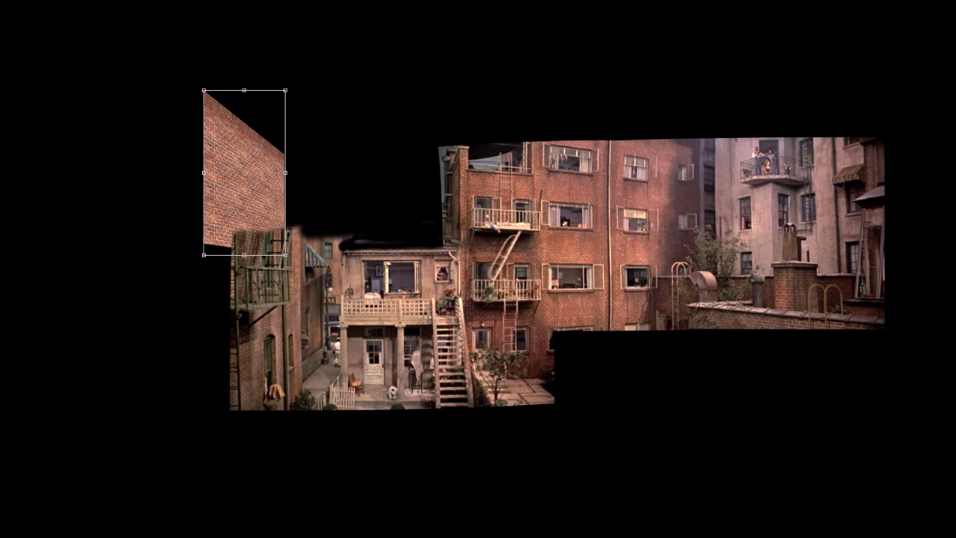
\includegraphics[width=\textwidth]{images/rearwindow-2.png}
\caption{}
\label{fig:rearwindow-compositing-1}
\end{subfigure}
\begin{subfigure}[b]{0.475\textwidth}
\centering
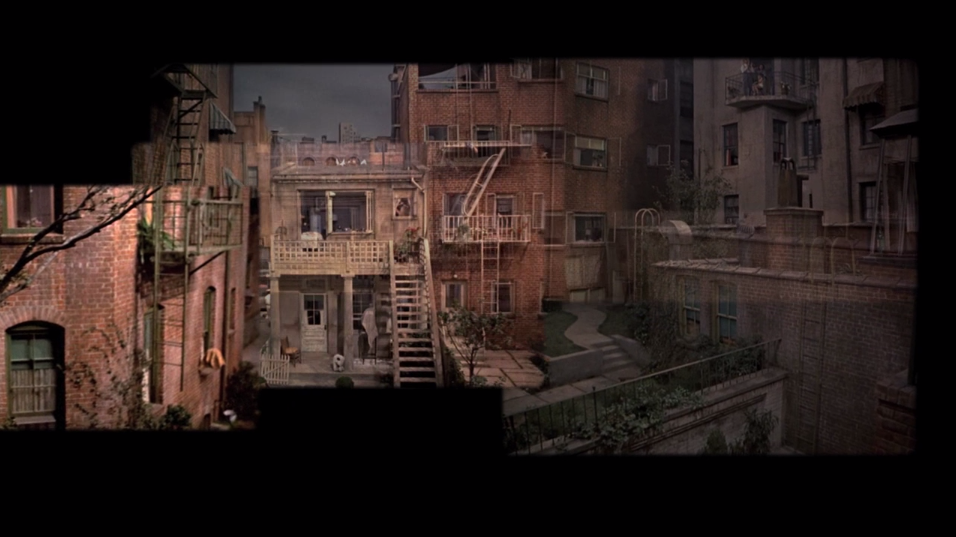
\includegraphics[width=\textwidth]{images/rearwindow-1.png}
\caption{}
\label{fig:rearwindow-compositing-2}
\end{subfigure}
%\begin{subfigure}[b]{0.325\textwidth}
%\centering
%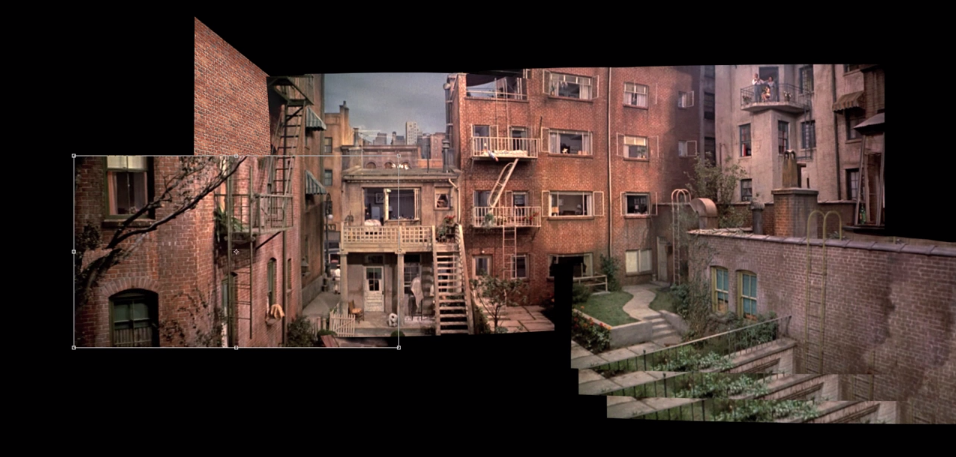
\includegraphics[width=\textwidth]{images/rearwindow-3.png}
%\caption{}
%\label{fig:rearwindow-compositing-3}
%\end{subfigure}

\begin{subfigure}[b]{0.96\textwidth}
\centering
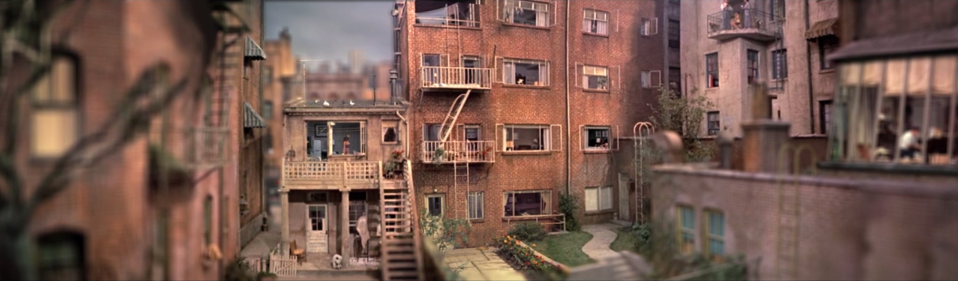
\includegraphics[width=\textwidth]{images/rearwindow-4.png}
\caption{}
\label{fig:rearwindow-compositing-final}
\end{subfigure}
\caption{A few frames from Jeff Desom's \textit{Rear Window Timelapse} showing the compositing process in Figures \ref{fig:rearwindow-compositing-1} and \ref{fig:rearwindow-compositing-2} to produce the seamless composite in \ref{fig:rearwindow-compositing-final} (reproduced with permission from the artist)}
\label{fig:rearwindow}
\end{figure}
% http://interactive.nfb.ca/#/outmywindow/
In another variety of digital media collaging, Jeff Desom takes individual shots within Alfred Hitchcock's \textit{Rear Window} taken by the main character in the story, Professional photographer L.B. "Jeff" Jeffries who is wheelchair bound, and reassembles them as a giant panoramic time-lapse view of his backyard in \textit{Rear Window Timelapse}\footnote{\url{https://vimeo.com/37120554}} (2012).  The compositing process is shown in Figures \ref{fig:rearwindow-compositing-1}-\ref{fig:rearwindow-compositing-2} to produce the seamless composite in Figure \ref{fig:rearwindow-compositing-final}.  As can be seen, there are no rough borders or edges where the individual frames were blended together.  The composite image plays as though the film had been shot in widescreen in the first place, though all the content came from only much smaller shots from the actual film.

JK Kellers' \textit{Realigning my thoughts on Jasper Johns}\footnote{\url{https://vimeo.com/37127916}} (2013) creates vector-based collages of the introduction for the television animation series, \textit{The Simpsons}, using a variety of features within Adobe Illustrator to vectorize the original image.  The artist describes his process with the accompanying video as first ripping each frame, then turning the rasterized images into vectors and using a variety of alignment and distribution tools to sort the vectors spatially.  He further describes a similar process for the audio where he takes images of the spectrogram and applies similar manipulations in Illustrator.  The self-described result is a ``frenetic mess of sight and sound''.

James Kerr appropriates images ``found here/there on the internet (a lot taken from northern and early renaissance paintings)''  within his animated digital collages \cite{Kerr2013} created using the Graphics Interchange Format (GIF), a common image format created in 1987 supporting simple frame-based animations supported by virtually all browsers \cite{Compuserve1987}.  The GIF format makes it easy to see animations anywhere in a web page as they are often embeddable in other common social networks such as Facebook and Twitter.   Petra Cortright uses GIFS of various emoticons within her website to create landscapes together within the interactive online browsing experience\footnote{\url{http://www.petracortright.com/}}.


\paragraph{Computational Art} 

Early computational artist Freider Nake recently said of computational artwork that it is ``thinking of infinities'', referencing an early work by A. Michael Noll, \textit{Gaussian Quadratic} (1965) which shows a line drawing output of an algorithm attempting to create all possible polygons, or his own work, \textit{Matrix Multiplication} (1968) which is described by an algorithm for matrix multiplication.  In algorithmic artwork, he states, the artwork is separated by its ``surface'' and ``subface'', where the procedural or computable definitions of the artwork are the subface, and the object exhibited or viewed by a participant is the surface.  We borrow the distinction offered by Nake and temporarily overlook distinctions between the terms algorithmic, computational, and generative artworks.  Such artwork are then described by subfaces consisting of procedural definitions capable of computing multiple surfaces.   Generally, this work will also refer to artists writing code to create new software rather than only using the defined capabilities of existing software.   The interested reader may be curious to research their distinctions and more recent ones such as computer art, digital art, pixel-based art, electronic art, media art, processual media, or new media art, which we do not extend upon within this thesis.%Importantly, this distinction raises concerns for describing artworks, as there are the procedures themselves which one could describe and the outputs they produce.  

Software such as Adobe Director, Adobe Flash, VJamm, VDMX, Apple Quartz Composer, Cycling '74's Jitter, Resolume's Avenue, VVVV, Modul8, Algoriddim's VJay, or Processing have created greater possibilities for video-based media than standard non-linear editors such as Adobe Premiere or Apple Final Cut Pro could offer \cite{Jaeger2006}.  These tools opened video-based practices to real-time and performative practices within Visual Music and VJ cultures, allowing one to design the output of their work (i.e. the surface) using procedural definitions (i.e. the subface).  Many Visual Music and VJ artists even created their own software, releasing them to the public such as Matt Black of Coldcut, who created VJamm, Netochka Nezvanova who wrote Nato.0+55, Miller Puckette, author of pd \cite{Jaeger2006} or the first VJ mashup tool VuJak, created with Cycling '74's Max/MSP.  Though these practitioners did not employ collage solely, it was certainly common of VJ practitioners to use fragments of existing material in the form of found video footage and mix them.  

In another variety of collage-like practices, Joseph Nechvatal's computer-robotic assisted paintings such as \textit{Birth of the Viractual} (2001) contains elements of a portrait being ``eaten'' away by computational processes.  The individual generative ``viruses'' create distinct boundaries that could easily have been individual pasted elements, though are only created through the dynamic time course of the individual processes.  Thus, more often than collage, the notion of generative or viral painting applies to Nechvatal's work.  However, one may be able to argue that the paintings are a collage of procedures (i.e. the generative processes, or individual viruses), modeled through their own collage-based set of rules (i.e. each individual virus will ``eat'' another pixel by copy-and-pasting from other ones).  

Ben Bogart's development of \textit{Context Machines} similarly resembles a collage of procedures, one which he describes as metacreation: ``the artist manifests the concept in a system whose output is presented to the audience. This is a process of metacreation: the building of systems that create media artifacts'' \citep[p.115]{Bogart2013}.  His work combines computational models informed by cognitive models and creativity theory in order to generate artworks deemed ``creative''.  His works explore computational models of ``conceptual spaces'' through the use of pattern recognition techniques such as self-organizing maps applied to large corpora of images.  The resulting outputs resemble dream-like collages creating surprising associations within everyday scenes.

%Demoscene is a thriving community of artists making use of different hardware configurations, often limiting their system requirements to smaller memory sizes and bandwidths.  The goal is often to write code that can still function despite the limited functionality of the hardware, also combining rules for generating audio.  

%\hl{Lev Manovich's Soft Cinema} see \url{https://en.wikipedia.org/wiki/Database_cinema}

\textit{Software studies}\footnote{\url{http://lab.softwarestudies.com}} (2007) has evolved the practice of exploratory data analysis to integrate the visual medium into its visualizations.  Its creator, Lev Manovich, calls it ``cultural analytics''.  Though sharing close ties to existing information visualization practices, visual analytics, and visual data analysis, its doctrine, so to speak, encourages (1) the use of the visual medium in existing graph-based approaches to information visualization, (2) the use of large multimedia databases and content-based information retrieval techniques, and (3) introducing these techniques to traditional humanities scholars through open-source tools.  Some of the lab's work includes visualizations of 1,000,000 manga pictures, 4535 Time magazine covers (1923-2009), and 62.5 hours of game play from ``Kingdom Hearts''.  These works were also exhibited in calit2 in the University of California San Diego campus where a 287 megapixel visual supercomputer is housed \cite{Manovich2008}.  In a similar vein, \textit{Phototrails} \cite{Hochman2013} explores the visualization of 2.3 million Instagram photos using radial plots sorting the hue and time of day though does not go as far as the \textit{80 million tiny images} project \cite{Torralba2008} which similarly creates impressive visualizations (it could fall under the umbrella of cultural analytics) but also develops a state-of-the-art scene classification algorithm using the dataset's existing image labels.  These examples demonstrate the power of collage in not only forming arts-based dialogues but also contributing to science through an exploratory analysis of information.  We will see a similar development in Chapter \ref{ch:synthesis-audio}, when we apply auditory scene synthesis for exploratory visualization purposes in a similar manner to these aforementioned examples.

%\hl{Computer Graphics -> boundaries of collage become less clear: https://www.youtube.com/watch?v=fw3XyOyl47Q}
%\paragraph{Visualization}

\paragraph{Web} Countless other examples of collage can be discussed when considering web-based practices, including Andruid Kerne's \textit{Collage Machine}, I/O/D's \textit{WebStalker}, or Mark Napier's \textit{Riot}, which attempt to use the imagery provided by online websites within interactive online collages.  Of particular note is Teehan+Lax Labs's \textit{Hyperlapse}\footnote{\url{http://hyperlapse.tllabs.io/}} which appropriates Google Street View's unique collection of 360 degree panoramic imagery rediscovering the original path the ``Google Van'' had taken in capturing the images.  The effect reproduces a time-lapse montage with points of focus following a blooming cloud, a plane in flight, or the CN Tower amidst a varied set of background objects.

\paragraph{Mobile Smartphones} Ubiquitous and embedded computing devices have exploded in the last 5 years.  As a result, the iOS App Store and Android Play have increasingly become platforms for finding works manipulating a user's own media stored on their device or through the use of the inbuilt camera.  Pic Collage\footnote{\url{http://pic-collage.com/}} has a reported 14 million downloads in its 1.5 years of being on the iOS App Store.  The app allows users to composite their images using ``freeform collages, cutouts, filters, borders, stickers, and text\footnote{\url{https://itunes.apple.com/app/id448639966}}.''   Countless other collage apps creating manually positioned collages can be found on the App Store with a simple search of ``collage'' including: FrameMagic, DecoSama, Shape Collage, InstaCollage Pro, Pic Joiner, Pic Stitch, or Pic Collage.  Mosaic apps are also in abundance, e.g. Mozaikr, Picasaic, Photo Mosaic Maker, or InstaMosaic.  These restrict the size of the fragments to pixel-like units, where the average color of an image is used to create one pixel of a larger image.  The mosaic is created using the library of images on the user's device.  Panorama makers are also in abundance, with Microsoft's PhotoSynth perhaps being the most popular.  %Painting apps such as AutoPainter HD by Mediachance do not go as far as producing collage-like aesthetics, nor do they incorporate source material for creating the filtered images.  However, their 

%\paragraph{Visual Display} 

% RML? http://www.barrythrew.com/projects/recombinant-media-labs/ .. could discuss different screen presentations, lead into augmented reality? immersive displays?

% Augmented reality?

\subsubsection{Sound Culture}
\label{sec:sound-technology}

% berliner 1887; edison phonograph, as archival, recording technique; gramophone; russolo, intonarumori; laszlo moholy-nagy 1923; lomax 1930's; fischinger 1932; levin 2003 ... 

\paragraph{Sampling} 
For sound, collage-based practices exploded with the birth of digital sampler hardware, coming only a few years after the mellotron, a similar machine which used analog tape instead of digital representations.  Similar to the practice of collage or montage, sampling\footnote{though refer to \cite{Navas2012} or \cite{Manovich2001} for a greater history of the term} refers to taking portions of existing media and using it within a performance or composition.  Digital sampling refers to sampling after an analog-to-digital process, where physical vibrations of sound are digitally sampled at equally spaced intervals, creating a discretely sampled representation of the continuous real-world phenomena.  This discrete sampling can easily be encoded by 1's and 0's in computer storage, and easily decoded back to the physical world, via a digital-to-analog process, such as through a speaker.  

Early digital samplers such as the Fairlight CMI to more recent non-linear editors such as Logic and Ableton Live have made multi-track and cut-and-paste operations trivial to accomplish, while visualizing sound waves has made finding relevant parts of an audio file relatively easier than listening to an entire tape reel.  Early adopters of digital sampler technology include Herbie Hancock and Public Enemy.  Founders of Dub, Lee ``Scratch'' Perry and King Tubby, also made use of existing recorded material.  Though not strictly sampling, they created the famous Dub sound by infinitely collaging the same sound, creating intense reverberations that echoed with greater magnitude on each bounce until the sound was cut.  

In 1987, the KLF produced ``What the Fuck Is Going On?'', which made extensive use of samples from The Monkees, The Beatles, Dave Brubeck, Led Zeppelin, Whitney Houston, and ABBA, amongst many others, citing on the album liner notes that the samples had been freed ``from all copyright restrictions''.  Despite their claims, their independent release was ordered to be destroyed by the Mechanical-Copyright Protection Society, leading to a re-release of the album with periods of protracted silence in place of the unauthorized samples.  They also released a guide including a detailed construction of how to reproduce the sound of the album, including the hardware used: an Apple II computer, a Greengate DS3 digital sampler peripheral card, and a Roland TR-808 drum machine.  

Two years later in 1989, John Oswald released an amalgamation of sampled music in his album, ``Plunderphonics'', including a visual reference to Michael Jackson's ``Bad'' on its album, which featured a derivative image of Jackson's original album cover for ``Bad'' edited to make it look like Jackson was a naked woman wearing a leather coat.  On the album, a song by the name, ``Dab''  was collaged to create the essence of a Michael Jackson track, using samples from Jackson's ``Bad''.  Oswald describes his process of sampling as using ``plunderphones'', describing them as, ``a recognizable sonic quote, using the actual sound of something familiar which has already been recorded'', satisfying the essence of being a plunderphone ``as long as you can reasonably recognize the source'' \citep[para. 10]{OswaldInterviews}.  In his writings available online, he further describes his motivations: ``'Plunderphonics' is a term I've coined to cover the counter-covert world of converted sound and retrofitted music where collective melodic memories of the familiar are minced and rehabilitated to a new life'' \cite{Oswald1985,J2013,Steenhuisen2005}.  Oswald's collage-based practice also extended to text, taking cut-up fragments from existing authors without citation, even including un-cited quotes to his own previous text ``Plunderphonics, or Audio Piracy as a Compositional Prerogative'' in ``Creatigality'' and ``Bettered by the Borrower'' \cite{Tholl}.   

Unfortunately for Oswald, the Canadian Recording Industry Association ordered him to cease-and-desist production and to destroy all remaining copies of ``Plunderphonics''.   In a similar fate as Oswald, sound collage artists Negativland in 1991 were sued by the pop band U2's label, Island Records, for their use of the trademark ``U2'' on the album cover and their sampling of U2's 1987 song, ``I Still Haven't Found What I'm Looking For''.   They also coined the term, ``culture jamming'' on their record \textit{Over the Edge, Vol. 1: JAMCON '84} \cite{McLeod2011b}, a phrase which they describe as ``a much needed form of self-defense'', because, ``art and commerce have now merged to a degree where corporate commerce now finances, grooms, directs, filters, manufactures and distributes almost everything we know of as `culture''' \citep[p. 13]{McLeod2011a}.  

Perhaps the most pervasive and popular use of sampling, or creative plagiarism as Kembrew McLeod cites it \cite{McLeod2011}, however, came in the form of Hip-Hop music.  Public Enemy's song, ``Caught, Can I Get a Witness?'', released in 1988, remarks on the practice of digital sampling: 
\begin{verse}
Caught, now in court 'cause I stole a beat\\
This is a sampling sport
\end{verse}
McLeod suggests that Hip-Hop's golden age of sampling occurred from 1987 - 1992.  During the case of \textit{Grand Upright Music vs. Warner Brothers Records} (1991), the judge stated ``Thou Shalt Not Steal'' in his opening remarks.  The lawsuits set a precedent for major record labels, and until today, it is standard practice to clear every sample used in a recording by legally licensing every use of copyrighted material, despite the possibility of it being determined legal after a fair-use argument.  With such practices in place, Kembrew McLeod and Peter DiCola hypothesized that the pervasive sampling of earlier works such as the Beastie Boys' \textit{Paul's Boutique} or Public Enemy's \textit{Fear of a Black Planet} would have lost nearly 20 million dollars even after having sold 2.5 million units \cite{Fassler2011}.  


\paragraph{Granular Synthesis} 
Within sound practice, a wide-number of practitioners have adopted the technique of granular synthesis.  This approach to generating sound works with an existing sound file or entire library of sounds and segments the files into ``grains'', or tiny fragments of sound generally lasting up to 50 ms.  The grains are collected and depending on the application can be time/pitch stretched/shifted, attenuated, crossfaded, looped, and/or distorted in any number of ways before they are reassembled based on either an interactive controller controlling the selection of grains such as a mouse or through chance operations.  Granular synthesis has seen wide-adoption since its early analog equivalents (as discussed within Iannis Xenakis' practice earlier in Section \ref{sec:collage-beginnings}) and have become staples in most digital audio production tools such as Ableton Live (e.g. Robert Henke's \textit{Granulator}\footnote{\url{https://www.ableton.com/en/packs/granulator/}}) or Propellerheads' Reason's \textit{Malstr\"{o}m Graintable}\footnote{\url{http://www.propellerheads.se/products/reason/index.cfm?article=devices_malstrom&fuseaction=get_article}} module combining wavetable and granular synthesis.  

\paragraph{Concatenative Synthesis} 
Concatenative synthesis extends granular synthesis by increasing the grain size thus also increasing the discernability of the original source.  Typically these are from 50 ms - up to any number of seconds, and can be layered by any number of segments to produce complex soundscapes, thus resembling the analog work of Schafer and Oswald (discussed in \ref{sec:collage-beginnings}).  First developed for the application of speech production \cite{Macon1996}, concatenative synthesis requires an analysis of sound segments where the analysis produces a description of each segment.  When creating a new phrase of speech, short samples of speech are matched to the phonetic text fragments to produce whole phrases.  

Concatenative synthesis was eventually extended to a range of applications within performance based settings.  Instead of using a text-to-speech approach, Diemo Schwarz used a mouse cursor to performatively select the individual segments within his custom interface \textit{CataRT} \cite{Schwarz2008}, allowing him to create soundscapes in real-time \cite{Schwarz2010,Schwarz2011} similarly to the work of MoSievius which used N-dimensional ``sieves'' described by high-level psychoacoustic properties of sound fragments \cite{Lazier2003a}.   Concatenative synthesis could also be used with another audio file's analysis as input driving the concatenatation process enforcing continuity rules \cite{Schwarz2000}.  A similar work was developed in Musical Musaicing where not just continuity but other global properties of a musical sequence could be specified and used to retrieve existing sound fragments from a large database to create musical phrases \cite{Zils2001}.  

Other examples include the use of matching an input sound source to a database of a video's audio file, thus driving video playback, as in Sven K\"{o}nig's \textit{sCrAmBlEd?HaCkZ!} performance using a live microphone to drive Michael Jackson\footnote{\url{https://www.youtube.com/watch?v=eRlhKaxcKpA}}\footnote{\url{http://www.popmodernism.com}}; Grierson's WMD which cut up video footage of the 9/11 tragedy and would match to video fragments based on audio analysis \cite{Grierson2005} and expanded to incorporate a FFT-based video analysis and average frame difference shot detection in Plundermatics \cite{Grierson2009}; Soundspotting which automatically organizes audio collections (initially developed using self organizing maps) and allows the exploration of the collection through an external audio input \cite{Spevak2001,Spevak2002,Casey2009}; or Remix-TV which could use a live violin to drive Alfred Hitchcock's Vertigo and accompanying musical score \cite{CaseyICMC2007}.  Nick Collins also used the technique with an on-the-fly onset detector during musical performances allowing him to create rhythmic structures resembling breakbeats or dance music \cite{Collins2004} and paired it with a live visual performance using similar concatenations with Frederik Olofsen in their 2007 performance \textit{Klipp AV}.  A chronological chart of performance systems can be found up to 2006 in \cite{Schwarz2006} which has since expanded on an online website\footnote{\url{http://imtr.ircam.fr/imtr/Corpus-Based_Sound_Synthesis_Survey}}.  %As well, Nick Collins recently reviewed musical applications of the approach and we therefore refer the reader to his thesis for more information.

\paragraph{Atomic Synthesis} 
Lastly, a more recent synthesis technique, atomic synthesis, describes a reconstruction of an audio signal using a dictionary of simpler signals.  This technique falls under the blanket of compressive sensing \cite{Donoho2006c}, which attempts to describe any signal using a sparse representation of orthonormal basis functions.  This method is also denoted in the literature by dictionary-based methods/sparse approximation/sparse signal reconstruction, and has significant advantages for producing meaningful passages of sound (or images), as the sparsity enforces continuity of sound localized at a point in time.  The process attempts to build a dictionary of time-based signal atoms, essentially short fragments of sound with simple timbres, such that when they are added at sparse temporal locations, they resemble the target signal to approximate.   Though it has rarely been used for artistic purposes, it is described in \cite{Collins2011} for morphing and cross-synthesis, where a dictionary is learned from one set of sounds and used to synthesize another; used within a framework for sparse signal separation to produce Spencer Topel's \textit{Elementary Sources} (2011) \cite{Topel2011}; and is implemented using Matching Pursuits in a C++ creative-coding toolkit for sound practice, Maximilian \cite{MickGrierson2013}.   

\paragraph{Mobile Smartphones}
Bronze Format\footnote{\url{http://bronzeformat.com/}}, for instance, probabilistically remixes the music of Gwilym Gold using stochastic rules for re-generating the music, creating never-ending music.  The app demonstrates how using the power of the inbuilt CPU, the iPod era of music playback is no longer confined to pre-recorded tracks but can operate in an online or real-time manner.   In another real-time generation of sound, \textit{RjDj}\footnote{\url{http://rjdj.me/}} and its commercial spinoffs such as \textit{Inception The App} or \textit{Darknight Rises Z+} use the device's inbuilt microphone to create fantastical acoustic spaces.  Rather than purely defining rules for remixing prerecorded content, RjDj allows for remixing tracks online, creating triggers based on changes in sound, and mixing with the ongoing auditory environment using the microphone.  Lastly, Nick Collins' BBCut (``breakbeat'' cutting) allows one to remix their music using algorithmic splicing to create an impressive array of rhythmic styles (previously discussed in the context of concatenative synthesis) \cite{Collins2004}.   

%Stop Motion -> Jan {\v S}vankmajer -> Pink Freud: https://www.youtube.com/watch?v=5NPiOjFVQRc
%Vinyl -> DJ'ing
%VJ'ing (VDMX, Quartz Composer, Jitter, Resolume Avenue; VVVV; Modul8). EBN; Coldcut in the 90's who used nature videos such as monkeys jumping, beetles tapping, and plants opening and synchronized their motions to sound samples using VJamm. Eclectic Method using Algoriddim's VJay iPad app.


%Photo-silk-screen
%Photo-litho
%Real-time video 
%Computer Graphics
% Corel Draw, Director, Flash

%\subsection{Computational Arts}
%\label{sec:background-computational-art}

%Until now, we've seen how technology has reshaped the practice of collage in interesting ways.  We now focus on collage-based practitioners that do not just make use of existing technology, but also write their own software.  Such practitioners are often the creators of algorithms and offer new ways of procedurally manipulating media.  In many veins, these practices make use of techniques in \textit{synthesis}, which, across a range of computational practices, describes a technique for creating media.  In sound, this can mean generating soundscapes (e.g. \cite{Schwarz2010,Schwarz2011}), entire phrases of music (e.g. \cite{a}), vowels (e.g. \cite{a}), or even entire phrases of speech (e.g. \cite{Moulines1990}).  For visual applications, similarly, synthesis can describe a variety of approaches for computationally generating images describing types of textures or patterns (e.g. \cite{Cohen2000}), artistic renderings (e.g. \cite{a}), or for video, dynamic textures such as clouds or fire (e.g. \cite{Schodl2000}).  In this section, we limit our review of this expansive field to practices specifically described by collage-based techniques which therefore also require the use of existing content.  



%\hl{Michael Grierson's Plundermatics}


%\subsubsection{Visual practices}

%\hl{Should I include background on image/video synthesis including NPAR community, textures, dictionary, collage, ... etc...basically what is in the chapter on artistic stylization in previous work currently?  Or should I only focus on arts outputs here as I said I would?}


%\hl{Aaron Hertzmann; SIGGRAPH community; }

%\subsection{Audio Information Retrieval}
%\label{sec:background-audio-information-retrieval}



%By the 1950's, artists and composers would also engage with cybernetic approaches.  Ross Ashby's \textit{Homeostat} for instance created a ... Bruce Lacey ... Thus, it appeared with the advent of robotics and increasingly more prevalent control structures, most notably the computer, making art through collections or fragments of processes would become a defining aspect of computational practices.



\section{Relationship to Coding/Compression Practices}
\label{sec:coding}

Scene synthesis can also be summarized by coding processes.  In the context of this thesis, an \textit{encoding} attempts to store representations of an audiovisual scene using a model of representation based on human perception, while a \textit{decoding} attempts to describe the stimuli again (i.e. as a collage).  The terms encoding/decoding are certainly not without their history.  

In the 1940's, Shannon's mathematical formulation of a generalized communication system described the communication between a source and receiver through a transmitter and receiver, respectively.  The source encoded the message, and the transmitter would convert it to physical phenomena, thus introducing possible noise sources effecting the message.  Finally, the message could be received and decoded by any destination that was capable of recovering the message.  His developments formed the basis of Information Theory, and along with developments occurring in military technology would later be incorporated by Norbert Wiener in a seminal text on communication theory entitled, Cybernetics.  

Wiener's, ``Cybernetics; or control and communication in the animal and the machine'' \cite{Wiener1948}, describes a field of research, denoted cybernetics.  It evolved out of military experiments in the 1940's building feedback processes which repositioned actuators (e.g. missiles/guns) based on updated predictions (e.g. sonar/radar/filters).  As an example, a matched filter provided a template response of a radar signal (e.g. of a known target) and was matched at each radar sweep providing a new orientation towards a target.  This new orientation could then be fed back into the system which would then again perform a radar sweep, a matched filter response, and a new heading, \textit{ad infinitum}.  This process forms the basic idea of homing in missile guidance, and is a defining principle of reducing noise in the field of signal processing (i.e. it maximizes the signal-to-noise ratio of a known signal corrupted by additive noise).   

It has also been likened to processes of active perception by Wiener himself.  Wiener suggests that each movement of the eye and neuronal levels of processing leads towards an invariant object representation (discussed in greater detail in Chapter \ref{ch:conceptual-visual}).  This entire process, in Wiener's own words, ``brings [visual] information one step nearer to the form in which it is used and is preserved in the memory'' \citep[p. 135]{Wiener1948}.  Wiener's early insights into the function of the eye, neuronal processing stages, and internal representations supporting perception will be expanded upon more in this thesis.  I will attempt to motivate and model similar perceptual processes in the auditory and visual domains and use them within a collage-based practice.

Cybernetics provided a vehicle for mathematicians and biologists in the coming years (e.g. Ross Ashby, Gregory Bateson).  It treated individual humans, animals, machines, or in cybernetic terms, \textit{systems}, as individual entities whose inner functions were not measured by their own capacities, but only in relation to what could be communicated by its own outputs to other systems.  It offered a new way of thinking about complex systems in terms of the information that was measurable outside of the contained systems.  Cybernetics was also highly influential within the arts, as demonstrated by the gathering of scientists, technologists, and artists in the ICA exhibition \textit{Cybernetic Serendipity} (1968).

Early cyberneticians, information theorists, and others at the time would eventually form the basis for modern day Information Sciences, where encoding and decoding are still very much used.  For instance, it is used to describe the processes of information compression, where a very large file such as an image, document, or video must be transmitted or stored more efficiently.  To achieve this process, it is first encoded to a different, often more compact, representation by an encoder, only to later be decoded back into its uncompressed original form when it is retrieved or accessed.  Decoding occurs every time you listen to an (encoded) MP3 file, where the MP3-codec describes the representation for compression and the procedures for encoding/decoding to/from it (e.g. see \cite{Richardson2010} for MPEG/H.264 coding processes or \cite{Furht1995} for an early surgery including JPEG/MPEG/H.261 specifications).  A significant part of compression and coding processes is dimensionality reduction.  That is, moving from one representation to another which has less dimensions, while attempting to retain as much of the original content's meaning (for a review see \cite{Bishop2006}).  Of course, meaning is entirely subjective, or dependent on the task for which one is reducing the data.   We will see how this process occurs for both audio, image, and video data in the coming chapters for the purposes of describing perceptual processes through an arts practice, as it will be necessary to make sense of large amounts of data and interact with it in a real-time manner.  

These terms are also commonly used within the field of Neural Coding, where encoding attempts to describe the neural populations representing brain-based representations of an external stimuli and decoding attempts to work from the neural populations back to describing the stimuli as a whole again.  The field has grown significantly in the last 10 years due to its successes with decoding images, video, and sound, as well as the recent developments within brain imaging and pattern recognition technologies (for a review see \cite{Naselaris2011}).  

Certainly, the methods built in this thesis when viewed in terms of encoding and decoding rather than typical collage-based practices can be seen to reflect coding/compression processes.  The encoding processes leading to a particular representation are capable of expressing the original information, though within a different method of representation (e.g. for an image, typically pixels will be used; however, in this thesis, we will build an image using a set of psychologically-motivated representations).  When distorting the intermediate representation in some ways, the decoding is likely to have unexpected results.  We will see how this process can be used to create a variety of effects including artistic stylization of image/video or for producing hallucinations in Chapter \ref{ch:synthesis-visual}.  

% Moradi 2004
% Rosa Menkman 2010
% 
Similar practices have explored distortion within computational representations of media.  In glitch art, artifacts perceived as ``breakdowns'' in a system are exploited in creative and interesting ways \cite{Franke2013}.  For instance, \textit{datamoshing} refers to the practice of intentionally altering information within encoded file formats so as to produce distorted interpretations of that file when it is decoded.  The technique itself can be applied in many different ways depending on the codec used.  As an example, when using Motion-JPEG, a popular video codec, artists often remove a particular kind of ``keyframe'' which tells the decoder when it should update all of its pixels.  In between these keyframes, the decoder will not use the actual content of the video, but instead track the individual pixels from the previous keyframe so that new image content does not need to be created.  This effectively helps keep the file size down while maintaining the important parts of the content.  When an artist removes these keyframes intentionally, the image content is tracked into a new video frame where much of the content should have been updated, effectively tricking the decoder into thinking it does not need to update all of its pixels.  This has the effect of one frame bleeding into the other in what Peter Kirn describes as causing ``frames to melt into one another like wax'' \cite{Kirn2009}.   Perhaps one interesting feature of the effect is that many people are already familiar with compression artifacts (e.g. from poor bandwidth streaming where network packets encoding the keyframes may have been lost).  When the artifacts are appropriated for creative use, however, they can create subtle and targeted effects.  Artist Yung Jake demonstrates a variety of these in his music video for ``Datamosh''.  See Figure \ref{fig:datamosh} for an example where he moves Justin Bieber's face  with the motion of the next few frames.   He further explains the technique in his lyrics for the song:

\begin{figure}
\centering
\begin{subfigure}[b]{0.325\textwidth}
\centering
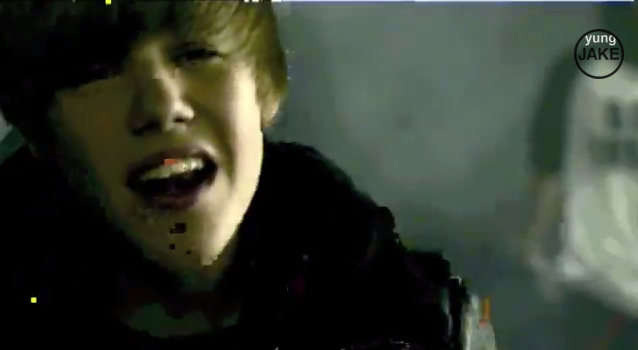
\includegraphics[width=\textwidth]{images/datamosh-1.png}
\caption*{Frame 1}
\end{subfigure}
\begin{subfigure}[b]{0.325\textwidth}
\centering
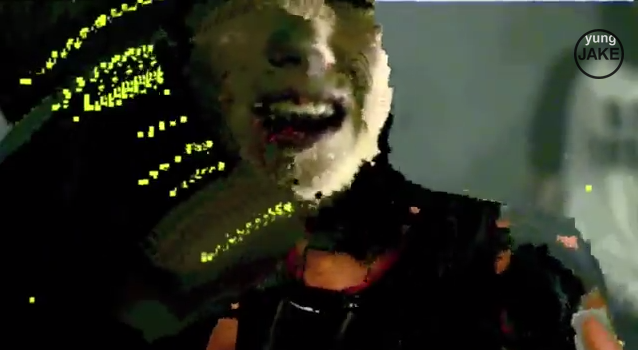
\includegraphics[width=\textwidth]{images/datamosh-2.png}
\caption*{Frame 2}
\end{subfigure}
\begin{subfigure}[b]{0.325\textwidth}
\centering
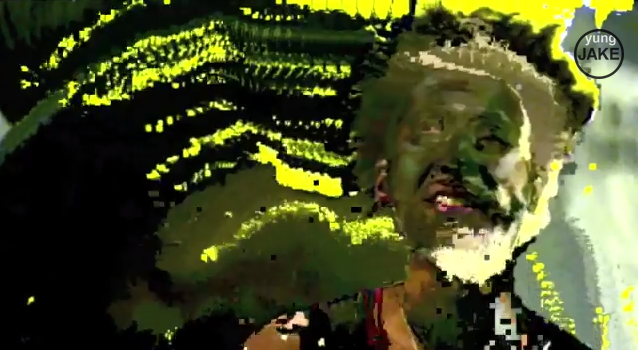
\includegraphics[width=\textwidth]{images/datamosh-3.png}
\caption*{Frame 3}
\end{subfigure}
\caption{3 example frames demonstrating datamoshing from Yung Jake's ``Datamosh'' Music Video located at  \url{https://www.youtube.com/watch?v=nS7QvOX8LVk}.  In Frame 1, Justin Bieber is displayed.  By removing a keyframe, Yung Jake is able to move Bieber with his own motions in the later frames, as shown in Frames 2 and 3.}
\label{fig:datamosh}
\end{figure}

\begin{verse}
Datamoshing cool, datamoshing great \\
Justin Bieber move him with my face\footnote{Jake is describing the effect from removing a keyframe where before there was a picture of Justin Bieber, and after there is Jake's own face.  The effect of removing the keyframe allows him to move Bieber's face with his own movements} \\
Then use it for an art show, use it for a piece \\
... \\
You thought it was an accident, a video glitch \\
I did it on purpose though... it's nothing \\
You don't have bad Internet, I'm just datamoshing\footnote{the effect resembles streaming artefacts from slow connections} \\
... \\
I'm on my datamosh, digital effects, man \\
I'm moshing data, geeked up can't stand\footnote{being ``on datamosh'', ``geeked up'', and ``can't stand'', suggests the effect has a drug-like power.} \\
\flushright{\textsc{Yung Jake -- Datamosh}}
\end{verse}

Other examples in glitch-based art are wide reaching and can be seen in a recent exhibition catalog \cite{Franke2013}.  To name just a few, \textit{pixel sorting} (coined by Kim Asendorf\footnote{\url{http://www.kimasendorf.com/about/README}}) describes a technique where pixels in an image are spatially sorted based on their values, or opening JPEG or other similarly encoded files in a normal text-pad and rewriting parts of it using normal keyboard letters.  This intermediate representation (i.e. the one viewed in the textpad) is not meant to be decoded by a text parser.  However, the interaction of writing text within this format is then stored back into the file, and when read by a decoder, viewed as an image.  The parts that were changed are likely unknown by the one manipulating the file, so there may also be a trial-and-error process.   Xra's \textit{Data Tragedy} (2012) allows one to enter a virtual world of glitch, posing as a DOS terminal game that corrupts itself after executing a few commands.  The process attempts to recall the participant's memory of the old operating system as well as first person shooter commands in order to complete the game.  Recent glitch-like aesthetics have even been commodified into the iOS apps GLTCH and Satromizer, offering effects such as Chop \& Screw, Melt, or Ghost. 

%\hl{relationship to virus?, transmediale 2003}

%\hl{Data tragedy (2012)}

% GLTCH and Satromizer (Ben Syverson) iOS apps
% Dan Tempkin. Glitch and Esolangs.  Brainfuck, Urban Muller, 1993. 
% data tragedy, memory of a broken dimension, 2012.  Ian Bogost.  Politics of game design is post-hoc.  Procedural representation and memory of representation as a gap.  
% Esoteric languages; Brainfuck.  Whitespace.  Unnecessary (keymaker 2005).  
% compressed sensing \cite{Donoho2006c}

% in order to trick the decoder into thinking a new refresh of the image content isn't necessary.  

% one's notions of the original compression with Jacques Perconte: http://www.electronfestival.ch/en/artist/159

%Dimensionality reduction...

%\hl{Composing an artwork through a collage of processes is certainly not a new one.  }

%\hl{Mick's thesis talking about software being composed of collage processes, visual programming environments vuo, maxmsp, jitter, qc, 4v, ....}

%\hl{Computational creativity, Boden, defining a successful work/evaluation... }

%\hl{Other cut-and-paste generative algorithms?}


%\section{Background in Information Retrieval}
%\label{sec:background-information-retrieval}

%Information retrieval is an expansive topic aimed at leveraging large collections of information.  Typically, one would like to access or retrieve a document from a large collection.  Information Retrieval as a field has grown to address better ways of solving this problem.  For instance, whenever you browse for files on your computer or use a search engine, you are using an engine for information retrieval.  Though this approach is typically described by ranked list described by textual metadata, the field has grown significantly due to advances in content-based approaches.  It is these approaches in particular that this thesis finds similarities with as they too aim to encode, represent, and decode a large set of material.  %Some philosophers have even gone as far as equating procedures within information retrieval to that of the human brain, though John Searle's Chinese Translation Room offers a thought experiment on how this may not be the case.

%\subsection{Visualization}
%Browsing purposes require dimensionality reduction... Multidimensional Scaling, Principal Component Analysis, Isometric Mapping, Self Organizing Map, Curvilinear Component Analysis, Laplacian Eigenmaps, Isotop, Samnon's Mapping, Locally Linear Embedding, Kernel PCA, Kernel Isomap.
%\subsection{Summarization}
%Clustering, Trees, Pyramids, Nearest Neighbors, Graphs, Lattices, Partitions, Ontologies, Kernel methods
%\subsection{Exploration}
%Ranked list, Clustering, Tree maps, Cone trees, Hyperbolic trees,... 

%\subsection{Image/Video Information Retrieval}







%\subsection{Media Libraries}
%As well, the amount of media has grown, and its access has only become easier with the advent of online archives such as YouTube, Flickr, Soundcloud, Freesound, just to name a few. 
% Shifting dialogue from war, communism, capitalism, to property, ownership, copyright
% in 1979 written about by douglas kahn, sad news by rob summers: https://www.youtube.com/watch?v=H4BmS9krF1A
%\subsection{Information Retrieval}
%\subsection{Information Visualization/Auralization}
%As collage also works with visualizing large amounts of existing data, the work also shares motivations with information visualization and information auralization, where the data are presented in order to tell a story.  

%In another vein, the work also shares motivations with encoding and decoding, or compression.  The purpose in compression is to take an existing dataset and reduce it down to ``perceptually'' similar information, while removing extraneous information.  
%In a related note, this process can also be used for encryption/decryption, where the same process is used to embed meaningful information that can only be deciphered through arcane processes, such as a table look-up or transformation of the data.  


%\section{Goals}
%\label{sec:goals}



%As this thesis approaches the understanding of perception from a conceptual, computational, and arts-based framework, the methods of evaluation may be seen at various stages.  It is important to realize the evaluation in the final arts practice.

%A set of parameters effect the two major modular components of the algorithm: attention modeling and representation.   Interaction is focused on the selection of material used in the collage, how the source content is parsed, stored, and for dynamic media, how the collage should be composited over time.  This system affords entirely new experiences around collage, such as the ability to aggregate source content in real-time or experience the collage through an augmented reality headset that mosaics the worlds as it is experienced.  

%\hl{Encode only parts of a scene that are likely to attract attention... motivate attentional model for dynamic content... }

%\hl{Develop representation of audio and visual corpus that affords simple interaction to produce different styles...}

%\hl{Fragments of a collage require precarious balance between what is identifiable, i.e. how discernible it is as the original source, and what can be composited, i.e. how it can fit within the greater context. }

%\hl{Difficulty of evaluating something subjective; not impossible; can measure performance of speed; art critics...}

%\hl{Model is beyond scope; more of a framework that can be expanded.}

\section{Outline}
\label{sec:overview}

This thesis attempts to open a dialogue surrounding the representations we use to support our ongoing scene perception through a collage-based arts practice.  Working in both auditory and visual modalities, the approach of this thesis is to first build a conceptual understanding of how we as humans support our perception through unconscious representations.  This framework will then inspire the development of a computational model.  Finally, we will develop an arts practice in order to better understand the shortcomings and successes of the model while opening a discussion around the nature of perception.  As designing a computational model of our perceptual systems within even one modality is a significant task, the goal of this model is not to accurately represent all possible levels of processing, but rather to focus on aspects of earlier levels thought to be unconscious or inaccessible to our conscious awareness.  The approach here is to work from the psychology, attempt to model aspects of the theory, and then develop the arts practice to reflect back onto the theory and modeling.

In the following chapters, a broad range of literature will be reviewed that has motivated such a representation.  Within audition, we will see that these representations are defined by \textit{streams}, and within vision, \textit{proto-objects}.  Despite their theorization, little attempt has been made to understand what an entire auditory or visual scene would sound and look like to our consciousness if represented in such a way.  This thesis therefore investigates their development within a computational method for audiovisual scene synthesis, an automated collage generation where the units of the collage are based on psychologically-motivated representations in perception.  

To produce a scene synthesis, two basic computational processes will need to be developed: \textit{encoding}, or storing learned representations of scenes such as images, videos, or sound files into memory; and \textit{decoding}, or matching stored representations to another set of scenes.  After developing the model for both sound and visual mediums, two artistic mediums will be explored in the final practice chapters.  The two practice chapters are separated by their functioning as an \textit{online} and \textit{offline} model.  Online denotes a real-time experience, where the result is interactively produced based on the ongoing environment.  This process often requires the algorithm to be designed in a more efficient way such that the processing required can interactively process without delay.  The online model attempts to demonstrate how the current stream of audiovisual information coming to a participant could be interpreted by our own perceptual systems using an immersive augmented reality to produce \textit{Augmented Reality Hallucinations} in Chapter \ref{ch:memory-mosaic}.  Offline, by contrast, means the process can occur over many hours and produce a result at a later given time.  Offline processing is therefore not restricted to design considerations in order to have the synthesis work in real-time.  We will see how an offline scene synthesis can produce more complex films using a significantly larger database from YouTube and more computational processing power to produce \textit{YouTube Smash Up} in Chapter \ref{ch:audiovisual}.  

This thesis will work through a modular approach.  At first, it may seem that a single architecture may suffice for both audio and vision.  However, these are fundamentally different domains that require individual treatment.  This means the thesis will first focus on developing scene synthesis for audio and then move on to developing another framework for vision.  Finally, the outputs of the two modalities will be combined in \textit{Augmented Reality Hallucinations} in Chapter \ref{ch:memory-mosaic} and \textit{YouTube Smash Up} in Chapter \ref{ch:audiovisual.  However, both the auditory and visual outputs will be built as separate modular frameworks in the hopes that their deeper connections (e.g. cross-modal and multisensory influences) could be explored in the future (discussed in more depth in the conclusion chapter).   This was chosen due to the fact that many open research questions still exist in defining even one of these modalities, let alone their interactions.  Some initial tests were done to develop their interactions, though it quickly became apparent that many more research questions would still have to be answered before convincing research could be conducted (also discussed in the final Chapter).  The combination of the two modalities as separate outputs will however give some insight for discussion in the future work section of the final Chapter.

To begin either module (i.e. audio and vision), a conceptual framework for unconscious representations in perception will be developed based on theory in behavioral psychology and electrophysiology (Chapters \ref{ch:conceptual-audio} and \ref{ch:conceptual-visual}).  This conceptual framework will then be modeled computationally (Chapter \ref{ch:analysis-audio} and \ref{ch:analysis-visual}) and developed into a scene synthesis framework for the purposes of developing automated collages (Chapter \ref{ch:synthesis-audio} and \ref{ch:synthesis-visual}).  The two modules will later be combined within an augmented reality to produce \textit{Augmented Reality Hallucinations} (Chapter \ref{ch:memory-mosaic}) and film to produce \textit{YouTube Smash Up} (Chapter \ref{ch:audiovisual}).  Finally, concluding thoughts on the contribution of this work, limitations, and future will be discussed (Chapter \ref{ch:conclusion}).  


%%%%%%%%%%%%%%%%%%%%%%%%%%%%%%%%%%%%%%%%%%%%%%%%%%%
%%%%%%%%%%%%%%%%%%%%%%%%%%%%%%%%%%%%%%%%%%%%%%%%%%%
%%%%%%%%%%%%%%%%%%%%%%%%%%%%%%%%%%%%%%%%%%%%%%%%%%%
%%%%%%%%%%%%%%%%%%%%%%%%%%%%%%%%%%%%%%%%%%%%%%%%%%%
%%%%%%%%%%%%%%%%%%%%%%%%%%%%%%%%%%%%%%%%%%%%%%%%%%%
%%%%%%%%%%%%%%%%%%%%%%%%%%%%%%%%%%%%%%%%%%%%%%%%%%%
%%%%%%%%%%%%%%%%%%%%%%%%%%%%%%%%%%%%%%%%%%%%%%%%%%%



%%%%%%%%%%%%%%%%%%%%%%%%%%%%%%%%%%%%%%%%%%%%%%%%%%%
%%%%%%%%%%%%%%%%%%%%%%%%%%%%%%%%%%%%%%%%%%%%%%%%%%%
%%%%%%%%%%%%%%%%%%%%%%%%%%%%%%%%%%%%%%%%%%%%%%%%%%%
%%%%%%%%%%%%%%%%%%%%%%%%%%%%%%%%%%%%%%%%%%%%%%%%%%%
%%%%%%%%%%%%%%%%%%%%%%%%%%%%%%%%%%%%%%%%%%%%%%%%%%%
%%%%%%%%%%%%%%%%%%%%%%%%%%%%%%%%%%%%%%%%%%%%%%%%%%%
%%%%%%%%%%%%%%%%%%%%%%%%%%%%%%%%%%%%%%%%%%%%%%%%%%%


\onehalfspacing
\chapter{Conceptual Framework for Building Unconscious Audio Representations}
\label{ch:conceptual-audio}
\minitoc
\doublespacing

\section{Introduction}

%\begin{quotationb}
%Most of us are brought up to feel that what we see out in front of us is something that lies beyond our eyes, out there. That the colors and the shapes that you see in this room are out there. In fact, that is not so. In fact, all that you see is a state of affairs inside your head. All these colors, all these lights, are conditions of the optical nervous system. There are, outside the eyes, quanta, electronic phenomena, vibrations, but these are not light, they are not colors until they are translated into states of the human nervous system. So if you want to know how the inside of your head feels, open your eyes and look. That is how the inside of your head feels
%\textsc{Alan Watts}
%\end{quotationb}

% What is the unit of perception that I can use across modalities and use in collage practice
% Global vs. Local in audio/vision
% Could do xyz, but did it this way...

%take examples in chap 1, what are unit, how does it approx percept of whole; how artists have thought about it... 

% pip/pop/ deviant

% road map to binding /crossmodal

% object files (wolfe), geons (biederman), indexical objects (pylyshyn), gestalts... need to motivate a process for discovering representations that are likely to be the units of attention

%Beginning with seminal theories of visual perception such as ``Gestalts'', ``proto-objects'' and ``Geons'' and seminal studies in Gist and Change Blindness, reinforcing what is known about early representations in visual perception, this chapter will then proceed into literature discussing auditory perception, focusing on research in Auditory Scene Analysis, fMRI, and the recording of electrical activity of the brain and Event Related Potentials (ERPs), leading to a discussion of representation in audition.  Finally, the review concludes in a discussion on developing a computational model of early perception using the presented theories.  



Our perception of the world is comprised of objects, events, and meaningful entities.  Yet, the sensory information we use to constitute these percepts are built from physical signals that have no meaning by themselves.  The challenge our perceptual machinery must face is associating this noisy incoming stimuli with meaningful entities we have already learned so that we may identify and utilize them.  This challenge was perhaps first described in the work of 19th-century empiricist, Hermann von Helmholtz, who suggested that the mind evaluates sensations through ``unconscious inferences'' which combine the stimulus of the world with prior notions of it to form our final perception. This process can also be summarized by two basic coding procedures: \textit{encoding}, or sensorial input as it is represented in our brains, and \textit{decoding}, or the perceptual experience as we interpret it.

To understand how coding processes may occur, numerous theories have proposed a representational framework for perception.  Such theories generally describe the encoding of the world within our brains using representations that are inaccessible to our consciousness, similar to the prior notions in Helmholtz's inferences.  As we do not have direct access to them, what might a representation supporting perception look like?  What can they explain, and what do they lack the ability to explain?  And how are they formed?  It is the aim of this thesis to open a dialogue around questions such as these through an arts practice focused on computational approaches to collage processes.  Within this collage-based practice, the units being assembled will be modeled based on the theoretical foundations laid in this chapter and the theoretical foundations for vision in Chapter \ref{ch:conceptual-visual}.  

This chapter is thus dedicated to (1) reviewing what is known about how representations in auditory perception may be coded and (2) describe a basic conceptual framework for their encoding and decoding using computation.  As the number of approaches to understanding perception are incredibly vast with many non-overlapping research areas, this review will sacrifice brevity for more depth in fewer areas of research, primarily describing research making use of electrophysiological techniques within cognitive neuroscience.  It should be noted that this thesis does not aim to replicate or extend these findings, as it does not use electrophyiosiological methods in its practice.  Rather, the intention is to only review this literature to motivate a few key concepts that will inform the implementation of a computational model.

In this chapter, we describe the notion of objects within auditory perception in order to understand what is entailed by a model of its processing.  From here, we will review a presiding theoretical approach for understanding objects: auditory scene analysis.  Within this theory, objects are known as streams, and do not necessarily relate to the objects we perceive visually.  We then discuss some key literature using electrophysiology which provide supporting evidence for brain-based representations of stream formations.  After reviewing this literature, we will be in a position to outline 4 key components describing a general conceptual framework for the implementation of a computational scene analysis model.  These will include: \textit{event detection}, \textit{segregation}, \textit{integration}, and \textit{template matching}.  We will develop these components conceptually in this chapter, and model them computationally in Chapter \ref{ch:analysis-audio}.

%We will see that literature describing basic components present in the brain, as measured by electrophysiology, gives rise to a understanding of a few basic components of processing.  These will be set forth in conceptual framework in the following chapter.

%\hl{rework this introduction to be clearer about my approach in this chapter, how it relates to building the computational model, maybe be explicit that this is auditory scene analysis, and a review of EEG helps to understand the basic components of building representations in the brain, though be clear that I am not using EEG in my thesis, just using this literature to build my framework which will be computationally modeled.}

%\hl{See if it makes sense to combine the next chapter on computational modeling the framework built within this chapter}

% Stress more about the practical aims, how this model will be used in natural, complex, real-world scenes... Give some examples... 
%As we do not have direct access to them, what do these representations look or sound like?  What can they explain, and what do they lack the ability to explain?  It is the aim of this thesis to build an understanding of perception through an arts practice focused on computational approaches to sonic and visual collage processes.  Within this collage-based practice, the units being assembled are modeled based on a theory of representations supporting perception motivated in this chapter.  The final aim of this practice is to open a dialogue around questions of representation within perception, thus reflecting back onto the theories set forth in this chapter.  

\section{Background Review on Auditory Perception}

\subsection{Defining the Auditory Object}

%talk more about bandwidth filters... work this into discussion and conclusion... 

We are capable of selectively listening to one of multiple sounds in an environment cluttered with simultaneous events, a feat known more colloquially as the cocktail-party problem \cite{McDermott2009}.  Consider the numerous sources of sound that are around us at any given time.  Each of these sources effectively produce waves of pressure that travel with different frequencies.  Each of these sounds eventually reach our ear to form a combined pressure wave with varying frequencies at any given moment.  Though we do not have eyes to move to different parts of an auditory scene, the cochlea of the inner ear can effectively break down the set of pressure waves coming to the ear which we perceive as sound.  These waves initially form a complex time-varying set of frequencies and are broken down into a set of narrow, ``critical bands'' \cite{Fletcher1940}.  From the energy in these bands, understanding how we represent and understand scenes within the auditory modality has been the main challenge of neuroscientists and psychologists investigating auditory perception.  

%\hl{Should probably discuss the physiology of the cochlea to auditory cortex a bit more.}

Certainly one challenge has been to define what the entities that compose the auditory scene may be described by within the auditory modality.  As Winkler points out \cite{Ist2010}, the notion of an object is highly guided by our visual experiences, and even the Merriam-Webster Dictionary defines object as, ``something that may be seen or felt'' (as quoted in \cite{Ist2010}) or as the Oxford English Dictionary puts it, ``something placed before or presented to the eyes or other senses'' (as quoted in \cite{Griffiths2004}).  

Griffiths notes that objects perceived must originate in the world, or else they are labeled as hallucinations or ``errors'' in processing in the brain.  Considering this fact alone might lead one to consider the auditory object as information leading to the \textit{source} of the object in the external world.  However, as Griffith continues to elaborate, the auditory object may also characterize information of an \textit{event} in the external world, and not necessarily provide information leading to its source or discrimination from other aspects in the current environment.  As an example, consider a voice in a crowd.  The source may be recognized as a particular speaker, lending information to the source of the sound and even where the sound occurred in space by matching to one's visual knowledge.  However, instead of the speaker, the vowels of the speaker may also be perceived, thus representing not the source of the speaker, but the auditory patterns of changes produced by different possible sources and in different possible environments \cite{Griffiths2004}.  

Perhaps a more useful definition of an object or of object-ness entails the capability of the brain to represent, attend, and understand complex and dynamic stimuli across what Marr in visual terms understood as \textit{variances} in a representation \cite{Marr1982}.  In other words, the perceivable object must be represented by some separable aspect of the environment.   It is perhaps due to the complex nature of defining objects in audition that the majority of the research in the last 40 years attempting to discover these separable aspects has focused on simple un-naturalistic acoustic scenes.  These scenes are generally composed of sine tones where simple physical parameters such as the tone's pitch or its temporal frequency may be altered.  Across modalities, this method of research has been denoted as ``psychophysical'', as the aim is to investigate the relationship of varying properties of a stimulus along one or more physical dimensions to a subject's experience or behavior. 

\subsection{Auditory Scene Analysis}

A seminal starting point into the study of auditory representation comes from psychophysical research in ``streaming''.  Van Noorden in 1975 demonstrated the bi-stability of perception when listening to alternating tones composed of sine waves \cite{Noorden1975}.  Depending on the tone's temporal frequency of onset, $\Delta \text{T}$, and difference in pitch, $\Delta \text{F}$, participants would perceive one of three possible scenarios: two separate streams (A tones and B tones, the \textit{segregated} percept); one stream (A and B tones, the \textit{integrated} percept); or a mixture of streams (the \textit{ambiguous} percept).  The integrated case is mostly demonstrated for a low $\Delta \text{F}$, the segregated case for high $\Delta \text{F}$ and/or $\Delta \text{T}$, and the ambiguous case for values in between.  Van Noorden describes the border between ambiguous and segregated percepts as the \textit{temporal coherence} boundary.  

Defining this boundary in greater detail has been the focus of research in the field of Auditory Scene Analysis for the last 30 years, a term coined by Albert Bregman \cite{Bregman1990}.  Approaches in Auditory Scene Analysis argue that the perceptual organization of an auditory scene is represented by a decomposition into pre-attentive auditory streams.  These streams are thought to be pre-attentive as we do not have awareness of them.  However, once a stream is selected by attention, or pops out demanding our attention, it enters our awareness.  For instance, if we are able to segregate sounds within a complex natural environment into one where we can describe a person's voice and what they are saying, then we will not be able to report information about other sounds that occurred at the same time in the environment.  In other words, the segregated stream that we can report has been \textit{foregrounded} by attention, bringing it to awareness, while the stream we are unaware of has been \textit{backgrounded}.  

Bregman argues that before streams are foregrounded, they are encoded by one of two formations: (1) rapidly available cues from primitive, low-level characteristics such as pitch, intensity, and spatial location; and (2), schema-driven integration of sensory evidence where schemas are defined by Gestalt-like regularities such as similarities, differences, common-fate, or continuity in frequency information from a continuous signal (discussed in more detail when reviewing the visual conceptual framework in Chapter \ref{ch:conceptual-visual}).  In the literature, these two formations have also been denoted, respectively, as \textit{simultaneous} and \textit{sequential} grouping strategies \cite{Winkler2009a}.  Simultaneous cues suggest that sounds are likely to be segregated if their physical characteristics are significantly varied despite their context.  As a result, these cues are independent of the attention of a listener and are purely based on the cues in the environment.  In contrast, sequential cues require a listener to have formed the notion of a representation, as the notion of regularity is based on previous listening.  These cues are more favorable in environments where very noisy conditions require precise knowledge of the source to attend to, thus resolving any ambiguities by using existing representations to segregate sources (e.g. the classic ``cocktail party problem'').  

Bregman's theory provides a basis for understanding the formation of auditory objects as they may appear within our perception as unconscious representations.  Rather than the notion of an explicit auditory object that must be defined by its physical characteristics, Bregman's streams provide a perceptual basis for representation as determined during auditory scene analysis.  Objects in the scene analysis sense are therefore based on the active analysis of a scene, i.e. what can be segregated at the given time based on the aforementioned cues, rather than any fixed description of an entity in the world.  

%\subsection{Behavioral Evidence for Auditory Scene Analysis}
%In attempting to understand whether humans encode auditory scenes like described by Bregman, we analyzed a set of 26 movies from the Dynamic Images and Eye-Movements corpus for a set of psychophysical measurements of sound.  As described in Section \ref{sec:diem}, this corpus includes highly precise eye-movement data collected from 48 participants... 
%Our findings are shown in Figure \ref{fig:diem-sound}.  

\subsection{Electrophysiological Evidence for Auditory Scene Analysis}

Research supporting the encoding of both of Bregman's theoretical formations of streams has seen great support through investigations making use of \textit{electroencephalograph} (EEG) recordings.   Before discussing research in electrophysiology, it is important to have a basic background in EEG techniques.  

EEG recordings, first described by Hans Berger in 1929, attempt to non-invasively infer brain activity by measuring a time varying signal of the electrical activity on the scalp of the head.  One of the benefits of EEG comes with its high temporal resolution often on the order of milliseconds.  To localize or disassociate changes in electrical activity in specific brain regions, more electrodes may also be used (up to 128).  As the raw electrical signals coming to electrodes are very low amplitude, the signals are first amplified.  However, the incredibly complex nature of the brain means that looking at the amplified signal may not be very useful by itself.  Thus filtering methods are often performed in order to limit the bands of frequencies within the recorded signal.  From here, understanding the relationship between the recorded signal and the external world can still be very tricky, as the world is full of events, and their relationship to the signal may only be present at very different times.  

Thus, a presiding technique of investigating brain activity using EEG in relationship to an external stimuli in cognitive studies is to time lock the recorded EEG in relationship to a specific event, a technique also known as the \textit{event-related potential} (ERP).  ERPs are simply the measured neural activity as measured in any electrode time-locked to the presentation of a stimulus.  By having many presentations, often denoted as trials, of the same stimulus, the average wave can be computed across trials for each electrode and then studied in greater detail.  

ERPs are generally described in terms of specific components that contribute to the averaged signal.  The nomenclature of some of the more basic components are based on their polarity (positive deflection, P; negative deflection, N) and how long after a stimulus they occur (e.g. N1 or N100 means a negative deflection around 100 ms after stimulus presentation).  
%s a result, many methods have been developed to express more meaningful measurements, such as measuring event related synchronization (ERS), which measures the magnitudes of different frequencies over time or component analysis, which attempts to re-project the EEG data into a set of hidden factors.  However, the 
%Some components are further named based on hemispheric considerations, such as a stimuli presented to the left side of the participant producing an ERP in the right hemisphere of the brain (contralateral, C), and where in the brain the ERP is generally found (e.g. a posterior or anterior contralateral component for vision, N2PC, or for audio, N2AC, respectively \cite{Gamble2011}).

\subsubsection{N1: Unconscious change detection}

One of the first well studied components within auditory processing is the N1 component which has been shown to be elicited during the onset of a stimulus (usually from silence to sound), providing evidence of a brain-based representation for unconscious change detection in auditory scenes.  Perhaps first described in 1939, Davis described a sound-evoked change in the EEG recordings of the waking human brain \cite{Davis1939}.  The onset of a tone evoked a negative wave 100-150 ms after onset near in the frontal-central locations of the scalp lasting for nearly 100 ms.  This was again described in a study in 1965 in which a flash of light or sound would proceed another flash of light or sound \cite{Sutton1965}.  Sutton et al. describes a negative potential peaking at 110 ms (N1) at the vertex of the scalp and a late positive potential at about 300 ms for sound and 340 ms for light (P3).  

Hillyard et al.'s 1973 study expanded on these previous results, showing that the N1 component is of even greater magnitude when a subject's selective attention is required in detecting a target tone \cite{Hillyard1973}.   In their study, a subject was presented random tones in either ear with very short irregular inter-stimulus intervals (ISIs, referring to the $\Delta \text{T}$), with higher pitch tones in the left than the right ear, and with randomly placed target tones with a slightly higher pitch in both ears.  The subject's task was to count the randomly placed tones in a target ear, meaning attention should have diverted to the target ear ignoring the other ear.  As a result, Hillyard et al. was able to demonstrate that the N1 component measured at the vertex (around 60-70 ms in most subjects) was of higher amplitude for events in the attended ear.  They suggested their results reflected an enhancement of the N1 component.  They also demonstrated an evoked late positive component peaking at 250 to 400 ms (P3) in the attended ear only when the target tone was presented, indicating the selective recognition of the target tone from which any subsequent cognitive or motor activities could follow (e.g. counting of the tones). 

\subsubsection{PN: Conscious template-match}

However, their result was later reinterpreted in another study which used longer ISIs of 800 ms \cite{Naatanen1978}.  Their study demonstrated that a new component, which they denoted the \textit{processing negativity} (PN), emerged exhibiting the effect of selective attention, rather than any enhancement of the N1.  This effect was found as a slow negative shift appearing at 150 ms and lasting 500 ms, rather than an earlier enhancement of the N1.  Their results indicate that the increased amplitude of the N1 in the attended ear could have been due to the short ISIs causing an overlap between the PN and N1 components, though even this explanation is still open to interpretation as a genuine enhancement of the N1 component can occur for strongly focused selective attention \cite{Naatanen1978,Hillyard1983,Naatanen2011}.  In any case, it seems the N1 is well described by the literature as an onset detector for auditory stimuli thus providing the awareness of a stimulus.  The PN may then provide an attentional-trace function, and be evoked during a template match during an attentional task requiring stimulus selection.  In other words, the PN shows supporting evidence for the brain's ability to retain representations and match them to incoming stimuli during a search task in a very short time.

\subsubsection{MMN: Unconscious segregation via sequential cues}

In 1976, another now well-known combination of components, the N2-P3a \cite{Snyder1976}, was demonstrated.  Unlike the N1 component which is based on the simple onset of a stimulus, the N2 was generated whenever a \textit{deviant}, or infrequent stimuli, was presented.  This difference became even greater with larger differences in Hz between the deviant and the \textit{standard}, or the stimuli that was presented more frequently.  For example, a tone would be presented with an 80\% chance of a standard 1000 Hz tone versus deviants of 1020 or 1040 Hz at 20\%).  This entailed the notion that some temporal regularity had been represented in order to compare it to the deviant stimuli.  Unlike the PN, the deviant did not need to be known or recognized based on prior training, or require selective attention, though its characteristics could effectively demand attention, hence evoking a P3a component peaking around 258 ms.  In contrast, when the subject was actively attending, a later P3 component denoted the P3b was evoked, peaking around 378 ms, still with the N2 component preceding it. 

The N2 component has since been very well studied, as it entails that we are able to represent the regularities of sounds and compare them to the ongoing environment evoking N2s whenever the regularity is violated even outside of a given task.  In particular, a re-interpretation of the 1976 study in 1978 showed that when subtracting the deviant trials from the standard ones, the remaining N2 spike (known as ``N2a'', thus making the original component combination now more commonly referred to as ``N2b-P3a'') demonstrates the brains capability to detect irregular changes in what the authors originally called ``template mismatch'' \cite{Naatanen1978}.  Importantly, these changes are not dependent on the deviant stimuli's features itself, but only in relation to the temporal regularities represented in the standard tones.  In other words, the template being matched to is likely an unconscious one, as the participant was not searching for it, nor were they aware of the deviant beforehand.  Rather, the standard set a predictive or inferential basis for any future irregularities.  

The remaining subtraction originally defined as the N2a was later denoted as the \textit{mismatch negativity} (MMN), and has been shown to appear anywhere from 100 - 250 ms after onset of a deviating stimuli \cite{Naatanen1978,Naatanen1987,Naatanen2007,Campbell2007,Garrido2009,Naatanen2011}.  Such relational negativities were also capable of appearing within the time-frame of the N1, originally leading it to be classified as a part of the N1 \cite{Naatanen1987}.  Though only recently has it has been discriminated from the N1 \cite{Campbell2007}.  The MMN's counterparts in other techniques for studying brain activity has also been demonstrated, including equivalents for magnetoencephalograph (MEG) \cite{Hari1984}, optical-imaging (OI) \cite{Rinne1999}, positron emission tomography (PET) \cite{Tervaniemi2000}, and functional magnetic resonance imaging (fMRI) \cite{Celsis1999}.  

Research demonstrating the window size of temporal integration has shown even for ISIs up to 350 ms, deviants in sequential tones can elicit a MMN during passive listening exercises (e.g. reading a book while headphones deliver the tone sequences) \cite{Tervaniemi1994,Tervaniemi1997}.  However, this window of integration can be prolonged to up to 500 ms during active listening, meaning attention is capable of prolonging the window of integration \cite{Kanoh2001}.  

The standard tone must also be established through repetition before a MMN can be elicited by a deviant \cite{Cowan1988}.  Interestingly, the amplitude of the MMN grows larger as the number of repetitions preceding the deviant gets higher \cite{Sams1983}.  This entails that the MMN represents a measure of the deviance established by the variances of the standard.   Further, it provides evidence suggesting that temporal regularities can be represented by the brain.  Research expanding on the MMN further has shown that more than low-level attributes such as pitch, temporal frequency, intensity, or duration, the same pattern of behavior is exhibited for a wide-range of stimuli even including higher-order or more complex violations such as timbre changes \cite{Tervaniemi1997a}, grammar in mother-tongue sentences \cite{Naatanen2001a}, or temporal sequences such as violations in patterns of ascending/descending tones \cite{Naatanen2007a,Garrido2009,Shamma2010}.

%When investigating measurements of MMN during segmentation and integration of sounds, the same pattern of activations are shown to exist for a single source as are for multiple sources, even when the sources share similar frequencies, suggesting that segmentation occurs before integration \cite{Sussman2005}. Such research suggests that pre-attentive processes within 150 ms provide a coarse shape or texture necessary for recognition, an auditory gist as the authors call it, and only the details that are necessary to the task at hand are further integrated \cite{Harding2007}.  

\subsubsection{ORN: Unconscious segregation via simultaneous cues}

Evidence for simultaneous grouping cues has been evidenced by research looking at the neural responses during listening of complex tones composed of inharmonicities \cite{Alain2001,Alain2002}.  Participants listened to a complex tone where all of the tones were either harmonic (i.e. all tones were multiples of the fundamental tone) or inharmonic tones (i.e. one tone was not a multiple of the fundamental).  The tones were also matched for perceptual loudness to ensure any differences were based on the complexities of the tone rather than a separate loudness cue.  Participants were given both an active and passive task.  For the active task, participants had to press a buzzer if they heard two separate tones.  For the passive task, participants read a book.   Participant's were at about 20\% chance of reporting that they heard 2 sounds when the mistuning was at 2\%.  This increased to 50\% at a 4\% mistuning, and 80\% for an 8\% mistuning.  The ERP data for active listening trials revealed an N1-P2 complex peaking at 110 and 200 ms over the central and frontal electrodes, followed by a late positive P3b component in the parietal regions.   Subtracting the ERPs to harmonic trials from inharmonic trials revealed that participants elicited a negative ERP component at 150-180 ms deemed the \textit{object related negativity} (ORN) in both active and passive listening.  This was followed by a late positive peak at 350-400 ms (P400) during active listening only.  The finding of an ORN in both active and passive listening conditions suggests that the detection of inharmonicities is an automatic process, though can be influenced by attention, as its amplitude in the active case was significantly larger than the passive one \cite{Alain2001,Alain2002}.

\section{Conceptual Framework}

Research behind the neuronal basis for memory representations, both conscious and unconscious, is greatly evidenced by research in electrophysiology.  This body of research suggests that (1) the ORN and MMN provide a neural trace of an unconscious memory representation; (2) the PN acts as a trace of a conscious one acting through selective attention; and (3) the N1 provides evidence for the brain's capacity for an unconscious stimulus onset detector.  Research demonstrating ORNs also provides evidence for the brain's capability for segregation via a simultaneous cue such as through inharmonicities, while the MMNs provides evidence for segregation via a sequential or schema-based grouping cue.  The schema for MMNs are defined by the temporal regularities of the standard, leading any deviances from this regularity to be segregated (with enough deviance).  With such deviants, the entire stream is not integrated into one concept, but segregated into two through an explicit measure of its deviance. 

Extending this research into a basic computational model requires at least: 
\begin{enumerateb}
\item \textbf{Event Detection}, such as evidenced by the N1, where an ongoing auditory stream is marked by an event boundary, allowing it to be encoded into memory.  This component is only necessary in models that do not have explicit event boundaries labeled for them; 
\item \textbf{Segregation}, as evidenced by the MMN and ORN, where the auditory stream is separated into foreground and background streams based on temporal irregularities;
\item \textbf{Integration}, the encoding process which stores the result of event detection, or if presented with enough deviance, the segregated auditory stream, into memory (whether or not segregation can occur before integration is certainly debatable, e.g. \cite{Sussman2005}, though for the purposes of this simplified framework, allowing segregation to occur before integration will have to suffice);
\item \textbf{Template Matching}, functionality as evidenced by the PN, where selective attention is capable of recognizing a stream as one that is the target of attention. 
\end{enumerateb}

Evidence demonstrating the elicitation of an N1 component suggests that as little as 60-70 ms are required before the brain is capable of detecting the onset of a stimulus event, even when engaged in another task.  This component demonstrates the brains remarkable ability to unconsciously detect a change in the environment.  It takes almost another 250-300 ms before we can become conscious aware of the stimulus onset, i.e. report the actual stimulus onset, as demonstrated by the P3 wave.  As a result, it seems that for developing an online analysis of an auditory scene, it is first essential to organize a real-time auditory stream into one chunked by discrete event boundaries.  

However, the literature discussing N1 elicitation does not seem to be clear on exactly how an onset may be modeled by the brain.  Each of the experiments reviewed above were designed with a streaming paradigm where short evoked tones were presented to a participant, meaning each tone was itself an event likely to be an onset.  Thus, each tone evoked an N1 response, as was demonstrated by averaged event-related potential measurements.  However, the real world is not aligned by events for us, making the notion of an event evoking an N1 outside of the psychophysical world of simple tones an unclear one.  How then does the N1 represent an event and determine when one has occurred?  Current approaches based on averaging ERP trials may not be able to answer such a question, as the notion of a change in the environment implies a violation of expectation.  By presenting the same auditory scene to a participant (e.g. in trials), the violation of expectation or the evocation of an N1 component, may become less likely.  In other words, the repeated presentation of the same stimulus may entail a more regular representation of the entire scene, making any deviations within it less ``irregular''.

Despite these issues, considering the groundwork laid by Bregman's Auditory Scene Analysis, one may be able to begin to define an onset detector based on the strategies of simultaneous and sequential grouping cues.  Though these cues up until now have been provided as evidence of cues for segregation (i.e. as evidenced by the ORN and MMN) rather than eliciting an N1 component, a re-interpretation of this theoretical foundation with the presented literature may allow us to apply the same framework for defining events in a continuous, real-world setting, i.e. defining onsets.  As a result, the ORN, MMN and N1 may share very similar strategies.  The major difference seems to be that the ORN/MMN are time locked to an onset, providing a basis for foreground segregation, i.e. the sonic environment before and after the N1 response, whereas the N1 may likely be based on an automatic time window.  It is unclear whether the N1 component is also activated for changes in the segregated foreground as may be represented by regularities required for the ORN/MMN, or if the N1 is only defined for changes in the entire acoustic scene.  It is likely though that the N1 may be able to consider any irregularity as a result of cues from either simultaneous or sequential grouping strategies, as it must act before both the ORN and MMN.  Given the research demonstrated thus far, it is also likely that this window is very short, e.g. within the timespan of evoking P3s, also considering the capability for detecting ISIs of up to 350 ms, though it is likely that this window size is also based on task/attentional demands.  

Another fascinating feature of the brain is its rapid capability of detecting a known sound, or a template sound, as illustrated by the PN.  What representation a template takes, or the time required before evoking a PN is still an open question, as the literature presented here did not look into complex environmental sounds.  However, the notion of a template match functionality does give us some evidence in proceeding towards a basic computational model.  Namely, it is likely that during selective attention tasks, the evocation of an N1 component must precede any detection processing of the target.  In other words, before knowing if a known sound has occurred in the sonic world, the onset of that sound must be detected via an N1 component.  Once the N1 is evoked, a PN component may be elicited if that particular event is detected as a match. 

\section{Discussion}

The literature presented here focused on evidence from cognitive neuroscience demonstrating some evidence towards the representations supporting auditory perception.  Specifically, this research primarily made use of electrophysiological recordings of subjects listening to psychophysical acoustic scenes composed of simple tones, and made use of repeated trials of the same scenes in order to measure ERPs, the average of simultaneous EEG recordings event-locked to a stimulus presentation (i.e. the individual tones).  

Taking this literature towards a scene synthesis requires building a collage where the units of the collage are based on similar units of representation processed by our perceptual systems.  We must therefore develop this conceptual framework into a computational implementation capable of representing an arbitrary complex acoustic scene into a set of units that may be manipulated.  However, the literature in developing an understanding of auditory scene analysis does not deal with complex acoustic scenes but is focused on unnatural psychophysical scenes composed of regular alternating tone sequences.  Only a few recent attempts have been made towards understanding brain bases for complex scenes \cite{Teki2011a,Teki2013}, where a ``stochastic figure-ground stimulus'' (SFGS) was created.  However, these studies are still modeled by unnatural sequences of randomly evoked collections of pure tones, and not modeled by natural scenes that have defined the literature as a whole, i.e. the cocktail party.  As a result, many assumptions are still made about the nature of what constitutes the auditory object.  

In these recent studies, the notion of figure is often placed on any aspect of the environment that is temporally coherent \cite{Shamma2011,Teki2011a,Teki2013}, assuming that these are the ``foregrounded'' aspects that we are likely to encode in an environment, as demonstrated by MMNs.  The authors assume that given the complex and unrealistic nature of their scenes, it is likely that a listener perceives an object consisting of integrated streams rather than segregated ones, as there is no prior notion to help segregate the stream.  That is, until a temporally coherent figure appears, providing a cue for a sequential segregation.  However, one important factor seems to be missing when considering any temporal regularities within a stream as being attentional ``foreground'', and that is the intricate relationship with the temporal \textit{ir}regularities in the stream.  As the conceptual framework I've laid out in this chapter demonstrates, any temporal regularity is only defined within the onset of a stimulus (e.g. the N1).  The onset itself must also be capable of also understanding irregularities in an environment.  As a result, any temporal regularity is only defined within the ability to define an event.  

Therefore, there is a multiplicity of regularities that must be considered: the first is defined by the onset detector (or N1), and is likely based on whole spectrum irregularities; the second is a segregation into foreground/background, using the time before and after an onset to define the basis for segregation.  As a result, a temporal irregularity within the whole spectrum must first be evoked before any temporal regularity within the segregated streams can occur, as there must be some basis for defining the event boundary.  Further, the notion of the temporal regularity past the irregularity must be sufficiently deviant from the preceding regularities before it is segregated, otherwise the entire stream is integrated.  

Considering this framework within SFGS stimuli, it is likely that many onsets are created during the time course of listening, even before the regular figure appears, since, by definition, the stochastic nature of the stimulus means there is a high chance of hearing something irregular.  Previous research has demonstrated that a standard must be set before a deviant can segregate the stream, albeit in simpler stimuli \cite{Cowan1988}.  As a result, it is likely that the statistics of the complex tones in SFGS are of high entropy, or high uncertainty, meaning many onsets could be evoked.  Within the onset then, it is likely that the time frame before and after the onset are composed of radically different tones, as they are randomly created.  It is likely then that many segregations can occur during the time course of listening, and not just one, during the highly regular set of tones, as the authors suggest.  

%Nevertheless, some understanding can be gained towards a practical computational model.  It should be stressed that this framework is not an accurate perceptual model, but simply one based on a basic understanding of some of the capabilities of our perceptual systems. 

\section{Conclusion}

The evidence presented thus far demonstrates the brains remarkable capability for detecting events in the sonic world and discretizing the continuous amalgamation of sound into units of processing where updates in representations may occur, or selective attention may discover a match.  Much of the literature to date has focused on either simple alternating tone sequences or random complex tone sequences, meaning many inferences must be made about how such evidence can be applied within complex natural scenes.  Nevertheless, some understanding can be gained towards developing a practical computational model capable of producing either segregated or integrated auditory streams.  

The conceptual framework presented here aims to build event-related units through a simple computational model beginning with an onset detection modeled after the N1 component.  From here, one of three processes may occur: matching, integration or segregation.  Matching occurs when a search task is involved and is modeled by evidence of the PN.  Otherwise, either integration or segregation occurs, defining the irregularities of the environment as it relates to the ongoing regularities.  This is in contrast to the N1, which likely requires some notion of regularities (as it must be evoked by an event that the sonic world has caused), but likely does not require segregation. WIth enough irregularity, a segregated stream may be defined, otherwise the stream is integrated.  

Future models should consider, at the very least: the numerous influences of stream formation by attention (e.g. \cite{Shamma2011}), whether integration should occur before or after segregation (e.g. \cite{Sussman2005}), categorical effects on low-level neuronal representations (e.g. \cite{Samson2010}), how encoded summary statistics from contextual influences may effect stream formation (e.g. \cite{Piazza2013}), and how this research may possibly translate to real-world natural sounds (e.g. \cite{Moerel2013}).  However, any one of these questions are all very active areas of research.  As a result, the basic set of components laid down in this Chapter can at least provide a plausible model from which a representation of auditory objects, or streams, may be built.  

The presented framework has given us the notion of the auditory unit of perception that can be used within a collage-based practice: namely, the auditory stream determined by auditory scene analysis as an integrated or segregated stream.  Further, during selective attention tasks, it has given us a notion of matching through a processing negativity, and that this matching process should occur within the timeframe of an onset.  We will develop these concepts into a computational framework in the next chapter, Chapter \ref{ch:analysis-audio}, demonstrating its use as a method for online source separation, browsing of a large corpus of audio, and for classifying auditory scenes.  This computational framework will then be developed for use within a collage-based practice in Chapter \ref{ch:synthesis-audio}, and combined with a visual collage-based practice producing computational audiovisual collages in Chapters \ref{ch:memory-mosaic}-\ref{ch:audiovisual} when discussing \textit{Memory Mosaic} and \textit{YouTube Smash Up}.

%Teki's recent work in 2011 and 2013 on complex scenes.

%Scenes are not like the classic problem they describe to simulate, instead are composed of simple scenes.  Needs to move past psychoacoustic scenes and understand realistic scenes.  


%Further, in real-world scenarios, it is likely that cues are given in both simultaneous and sequential formations.  As a result, some research has suggested that segregation may be understood in terms of temporal coherences.  These describe the formation of streams in terms of any incoherences within the set of possible cues coming from pitch, intensity, spatial location, or sequential groupings defined by Gestalt-like rules.  Shihab Shamma's work in modeling temporal coherences suggests that stream formation may be aided by attentional mechanisms.  Rather than stream formation occurring due to any incoherences in cues, attention may select one of many cues, and only then will other similar temporally coherent cues be bounded together.  Such an interpretation is still open to debate.  Yet, it does highlight the fact that the role of attention within stream formation is still very difficult to determine.   That is, unconscious representations may be mediated by top-down processes such as attention, task, and memory.

%Research in representations forming outside of selective attention has been given additional support through the phenomena of change deafness, termed similarly to change blindness as it shares some similarities (discussed in Section \ref{sec:change-blindness}) \cite{Vitevitch2000}.  Participants were instructed to repeat out loud a list of words as heard coming from one ear of their headphones, and to ignore the words presented in the other.  The words range from lexically easy words (high word frequency and few words are similar sounding) to lexically hard words (low word frequency, many words sound similar to it, and the similar sounding words have a high frequency of occurrence).  Halfway through the list of words, participants were given a 1 minute break, and the speaker's voice would change on only one of the trials.  42\% of participants (5/12) were unable to detect the change in speaker.  Unlike participants that did not detect the change, participants detecting the change had faster reaction times in repeating lexical words with decreased lexical difficulty though were unaware of the change in the speaker's voice.  This suggests that in order to detect the change, some increase in processing and hence the increased reaction time in repeating the word was required.  This increase in processing suggested that attention towards the auditory stimuli was required for detecting the change.  

%Research demonstrating change deafness opens questions into the nature of templates effecting MMN and PN.  The results could be interpreted that the original speaker had provided a template match providing a basis for segregation and hence the decreased reaction time, but had not been integrated to conscious awareness and hence no awareness of the different voice.  Another interpretation could be that the template is integrated, but cannot be automatically compared.  More recent research has expanded on its result showing that transients of white-noise or silence were not necessary to produce change deafness, unlike its visual counterpart \cite{TURATTO2008}.  Their results suggest the short-term auditory memory capacities were the main deciding factor of change deafness.  

%\subsection{Brain Imaging}

%May delete this section.

%How this process occurs neurologically in audition has only recently been investigated. In a study employing fMRI of subjects listening to random note sequences, activations shown in IPS and STS occur during ``figures'' of a less random nature than the preceding and following note sequences, though participants are unable to report hearing a figure, suggesting pre-attentive binding of spectral-time course information occurs during listening \cite{Teki2011a}. As fMRI scans typically take on the order of 2 seconds per scan, understanding if a subject is aware of a figure can only be done qualitatively after listening.  However, recent research investigating the attentional mechanisms involved in time-course encoding of auditory streaming paradigms often also make use of EEG recordings as the temporal precision required in understanding if and when attention acts upon a figure is on the order of milliseconds.  For example, evidence for the predictive encoding in time-course frequency information \cite{Winkler2009} give further evidence for the predictive encoding of figure-ground relationships.  As well, in investigating the endogenous influences on figure-ground encodings, subjects were given a task of reading a book while recorded for EEG.  Onsets of changing note patterns elicited mismatch negativities in primary auditory cortex, indicating grouping can occur outside of the task at hand.

%The research stemming from change deafness, auditory gist, and MMN have motivated that we are capable of producing unconscious representations in perception.  Further, these representations are even demonstrated across a wide range of modalities (visual MMN is discussed in Section \ref{sec:vmmm}) and further demonstrate the brains ability to segregate and in some cases integrate perceptual phenomena without the need for conscious awareness.  

%\subsection{Maybe}

%Should I mention/talk about developmental studies, music perception, natural scenes, soundscapes, musique concrete?




%%%%%%%%%%%%%%%%%%%%%%%%%%%%%%%%%%%%%%%%%%%%%%%%%%%
%%%%%%%%%%%%%%%%%%%%%%%%%%%%%%%%%%%%%%%%%%%%%%%%%%%
%%%%%%%%%%%%%%%%%%%%%%%%%%%%%%%%%%%%%%%%%%%%%%%%%%%
%%%%%%%%%%%%%%%%%%%%%%%%%%%%%%%%%%%%%%%%%%%%%%%%%%%
%%%%%%%%%%%%%%%%%%%%%%%%%%%%%%%%%%%%%%%%%%%%%%%%%%%
%%%%%%%%%%%%%%%%%%%%%%%%%%%%%%%%%%%%%%%%%%%%%%%%%%%
%%%%%%%%%%%%%%%%%%%%%%%%%%%%%%%%%%%%%%%%%%%%%%%%%%%


%%%%%%%%%%%%%%%%%%%%%%%%%%%%%%%%%%%%%%%%%%%%%%%%%%%
%%%%%%%%%%%%%%%%%%%%%%%%%%%%%%%%%%%%%%%%%%%%%%%%%%%
%%%%%%%%%%%%%%%%%%%%%%%%%%%%%%%%%%%%%%%%%%%%%%%%%%%
%%%%%%%%%%%%%%%%%%%%%%%%%%%%%%%%%%%%%%%%%%%%%%%%%%%
%%%%%%%%%%%%%%%%%%%%%%%%%%%%%%%%%%%%%%%%%%%%%%%%%%%
%%%%%%%%%%%%%%%%%%%%%%%%%%%%%%%%%%%%%%%%%%%%%%%%%%%
%%%%%%%%%%%%%%%%%%%%%%%%%%%%%%%%%%%%%%%%%%%%%%%%%%%



\onehalfspacing
\chapter{Computational Auditory Scene Analysis}
\label{ch:analysis-audio}
\minitoc
\doublespacing

%\begin{abstract}
%The growth of digital audio archives has built the need for intelligent content-based analysis systems.  Within audio archives, an acoustic class may not occur as an isolated stream but rather within a mixture of other acoustic classes.  As such, content-based information retrieval algorithms should also be capable of classifying the separate acoustic classes that give rise to an acoustic scene's mixture.  This paper investigates the performance of three classifiers; (1) a full-frequency and (2) reduced frequency classifier both built using a probabilistic variant of non-negative matrix factorization, probabilistic Latent Component Analysis (pLCA), which describes audio by the latent components that represent the signal, and (3) a Gaussian Mixture Model of one of the most common acoustic features, MFCCs.  We evaluate these models in a variety of cases: (1) classifying acoustic textures, (2), classifying acoustic textures in the presence of noise, and (3), classifying acoustic mixtures.  Both pLCA models outperform the MFCC-based model in cases (2) and (3), correctly classifying the mixture's sources 94\% of the time in comparison to 74\% of the time for the model built with MFCCs.
%\end{abstract}

\section{Introduction}

In this chapter, we develop the conceptual framework laid down in Chapter \ref{ch:conceptual-audio} into a computational model capable of two processes: \textit{encoding}, or the sensorial input as it is represented in our brains, and \textit{decoding}, or the perceptual experience as we interpret it.   These two processes will be necessary for developing an auditory scene synthesis, a collage-based synthesis where the units of the collage process are based on psychologically motivated representations thought to support perception.  To model these two processes, we need to develop our conceptual framework as described in Chapter \ref{ch:conceptual-audio}: 

\begin{enumerateb}
\item \textbf{Event detection}: Temporally segments the ongoing auditory stream in order to define the boundaries of processing.  This component is only necessary in cases where explicit events are not already defined; 
\item \textbf{Segregation}: In case an auditory stream is composed of a multiple streams, the mixed stream is split into a foreground and background stream; 
\item \textbf{Integration}: Encodes the segment by building an internal representation of the stream; 
\item \textbf{Matching}: Decodes the encoded stream by matching to a known template.
\end{enumerateb}

In the next two chapters, we work with fixed-length units of sound, and therefore explicitly define event boundaries.  In a corpus described by varying segment lengths or for a real-time setting, we would not have this luxury, and would instead need to use event detection to computationally discover the segmented units of sound.  In Chapters \ref{ch:memory-mosaic}-\ref{ch:audiovisual}, we will see how combining this framework with event detection affords greater expressivity for encoding and decoding when discussing \textit{Memory Mosaic} and \textit{YouTube Smash Up}.  

Our units of sound must still be encoded, represented, and decoded.  If the entire sound stream is to be integrated, then the unit defined by the event detection is encoded without further manipulations. However, if the unit requires segregation, then the unit is separated into a foreground and background stream, where the foreground stream denotes the stream that is integrated as a result of being ``selected'' by attention.  Finally, matching determines whether the current stream matches a previously learned target encoding, effectively allowing us to decode a stream based on prior learning.

%\hl{Really need to talk about existing auditory models, different frequency transformations, leaky integrators, phase, slaney, lyons,... }

In this chapter, we implement three computational methods for encoding and decoding.  These are described as (1) a full-frequency and (2) reduced frequency representation both built using a probabilistic variant of non-negative matrix factorization, Probabilistic Latent Component Analysis (PLCA), which describes audio by the latent components that represent the signal, and (3) a Gaussian Mixture Model of one of the most common acoustic feature representations, MFCCs.  As we will see, the first two models attempt to compute a basis decomposition of a time-frequency matrix into a set of components modeled by a set of frequencies with a time-varying amplitude, ideal for cases when segregation is required.  The last model on the other hand describes a set of frequencies by its overall spectral shape, taking into account the perceptual bandwidth given to different frequencies.  This spectral shape does not vary with time like the first two models, and is composed of only one set of values describing the global shape of the spectrum, making it ideal for cases when segregation is not required.

In order to evaluate each model's performance, we consider a common use-case outside of the context of scene synthesis which requires encoding and decoding routines: classification.  In particular, classification is often employed within information retrieval frameworks in order to attempt to aid the browsing and retrieval of content within large archives, a need that has grown due to the growth of digital audio archives.  As the notion of classification entails providing a semantic description of an auditory stimulus, it is important to be clear about what this thesis means by a \textit{class}, \textit{scene}, \textit{event}, and \textit{stream}.  A class semantically describes either a scene or event.  A scene defines a collection of acoustic events associated with that particular physical place.  As an example, one would expect to find events classified as ``honking'', ``engine noise'', and ``talking'', in an acoustic scene described as ``city street''.  A likely distinction between the term acoustic scene and acoustic event is that a scene is composed of many events, many of which could be of different classes, while an event is composed of only one particular class.  As a result, there is a many-to-one definition entailed by scenes, where many possible definitions can give rise to the same scene, and a one-to-one definition for events, where only one possible class exists.  The terminology of a stream enters when discussing a particular perception of that scene.  For instance, when listening to an acoustic scene, a stream would by described by what is encoded into memory (i.e. the entire scene, which may be segregated during particular events into foreground and background streams) and the resulting perception would describe what is decoded.  

An ideal information retrieval engine should be capable of classifying acoustic scenes, events, and when presented with complex scenes, also determine if simultaneously occurring events can be described.  For example, an auditory scene of ``party'' may also be composed of a ``hair-dryer'' in the background.  This additional class may make it difficult to describe the scene, unless it is capable of also segregating the scene into two classes.  An analogous model in vision is one that detects objects in a visual scene rather than the entire scene itself.  The difficulty of classifying the multiple events comprising an acoustic scene is well noted in acoustic event detection literature where classification performance breaks down from 70\% for classification of a single event in isolation to 25-40\% during mixtures of events or events presented with noise \cite{Temko2007}.  

With these distinctions in mind, after developing our models, we turn to evaluating them within the context of auditory classification by using a large audio corpus of labeled acoustic events in a series of experiments: (1) classifying isolated acoustic events, (2), classifying an acoustic scene comprised of one known acoustic event and an additional unknown acoustic event, effectively creating noise, and (3), classifying an acoustic scene comprised of two simultaneous events that are both known.  By known and unknown, we simply mean to say that the classifier has or has not encoded knowledge of this class in some way.  For testing purposes, this entails turning our 10 second clips into 10 folds of 1 second clips and performing cross-fold validation on 10 folds.  This entails encoding 9 folds and seeing whether this information allows the classifier to decode the last fold.  We will see that both PLCA models outperform the MFCC-based model in cases (2) and (3), correctly classifying the mixture's sources 94\% of the time in comparison to 74\% of the time for the model built with MFCCs.  However, for case (1), i.e. when a scene does not require segregation, all of the models perform with excellent performance.  This evaluation serves to highlight how each model may perform within complex auditory scenes composed of multiple events when it is later coupled with event detection in Chapter \ref{ch:synthesis-audio} to create a real-time auditory scene synthesis and finally in Chapter \ref{ch:audiovisual} when it is combined with visual scene synthesis.  


\section{Related Work}

Due to the amount of information contained in archives and the complexity in pre-processing so much information, the first step in a content-based solution to information retrieval is often to reduce the dimensionality of the data while keeping as many of the perceptually relevant dimensions as possible.  In audio, this often equates to looking at the distribution of frequencies that describe a signal (e.g. by taking the Fast Fourier Transform (FFT) of an audio signal) and computing features or a fingerprint which could be used to train models/classifiers.  Most previous work in acoustic classification and retrieval makes use of a combination of features described by Mel-Frequency Cepstral Coefficients (MFCCs) and low-level psychoacoustic descriptors \cite{Temko2007,Guo2003a,McKinney2003,Allamanche2001} such as spectrum power, centroid, zero-crossing rate, brightness, and pitch.  MFCCs were first described in a seminal study on automatic speech recognition \cite{Davis1980} as a perceptually motivated grouping and smoothing of power spectrum bins according to the Mel-frequency scaling.  MFCCs can be thought of as a perceptually motivated, reduced, and de-correlated representation of a frequency transform, and are approximations to the overall texture of an acoustic signal.  Hence, though MFCCs were originally applied to speech recognition problems, they are also widely used as audio features in the domains of general acoustic events \cite{Temko2007} and music \cite{Pampalk2006a,McKinney2003} analysis.  

% A number of viable solutions exist for music and sound based CBIR. \cite{} employs the use of psychophysically based descriptors such as loudness, brightness, and spectral centroid which are computed based on the physical moments of the frequency distribution.  Building a blah blah blah \cite{}.

% (Audio Classification Based on MPEG-7 Spectral Basis Representations; Hyoung-Gook Kim, Nicolas Moreau, and Thomas Sikora, 2004).  SVMs... GMMs (see 2008 paper by Hoffman using HDP and GMM of MFCCs).    

% The ability to segregate an acoustic scene and classify the simultaneous parts of a content allows for more descriptive analysis of stored data, such as which acoustic events appear within the scene (e.g. ``car'', ``horn'', ``talking'' versus ``street noise'').  However, 

Approaches building MFCC and low-level based descriptors into a large feature vector attempt to depict an auditory scene by a vector of global parameters. Thus distance measures attempting to perform matching and that act on the MFCC feature vector are generally unsuited for describing acoustic scenes requiring segregatation.  This is because any measures acting on the MFCC will penalize any deviation from the global feature vector's approximation.  In other words, approaches to auditory classifiers using k-means \cite{Harma2005,Eronen2006,Allamanche2001}, hidden Markov models \cite{Eronen2006,Mesaros2010}, support vector machines \cite{Guo2003a}, or Gaussian mixture models \cite{Wang2011,Aucouturier2007a,Pampalk2006a} aim to model the distribution of possible variants of a feature vector rather than the many possible subspaces that may define them. 

The MPEG-7 standard \cite{Casey2001a,Manjunath2002}, however, describes a modular approach to understanding the subspaces of such feature vectors by looking at their basis decomposition.  In this manner, our approach to modeling segregation most resembles models employing spectral basis decompositions which describe de-correlated features of an acoustic signal using principal component analysis and independent component analysis \cite{Casey2001a,Xiong2003,Kim2004}, local discriminant bases \cite{Su2011}, matching pursuits \cite{Chu2009a}, or non-negative matrix factorization \cite{Raj2010}.  However, our approach differs from the MPEG-7 standard's spectral basis decomposition \cite{Casey2001a} as we instead investigate a full-frequency and Mel-frequency decomposition, rather than decibel-power scale or de-correlated features, and further use a recently developed machine learning algorithm for discovering latent components rather than any of the aforementioned models.

In order to compute the basis decomposition of an audio signal's frequency transform, we focus on a recently developed method for latent component analysis based on probabilistic Latent Semantic Analysis (pLSA) \cite{Hofmann1999} called probabilistic Latent Component Analysis (PLCA) \cite{SmaragdisRajShashanka}.   PLCA has shown great promise for a variety of use cases including source separation and de-noising \cite{Smaragdis2007a,Smaragdis2007}, online dictionary learning for source separation \cite{Duan2012}, riff-identification \cite{Weiss2011}, polyphonic music transcription \cite{Benetos2011}, and classification during mixtures \cite{Nam2012}.  However, no detailed investigation of PLCA into the performance and applicability of classification for isolated or mixtures of classes in comparison to a standard MFCC model exists.  Further, previous investigations of PLCA for source separation and classification only make use of the full-frequency spectrum in a limited number of classes, and PLCA's applicability for reduced frequency representations is still unknown.  We therefore investigate the performance of 2 models built using PLCA (full-frequency and reduced) through 3 experiments in acoustic classification while comparing it to a classifier based on the well known Mel-Frequency Cepstral Coefficients (MFCCs): (1) classifying isolated acoustic events, (2), classifying acoustic events in the presence of an untrained event, effectively creating additional noise, and (3), classifying acoustic scenes composed of two simultaneous acoustic events.  

\section{PLCA}
\label{sec:plca}

The underlying basis of the standard PLCA model was first proposed in \cite{Hofmann1999} as a probabilistic extension to Latent Semantic Analysis (LSA) called probabilistic Latent Semantic Analysis (pLSA).  Singluar Value Decomposition (SVD) based LSA methods and their non-negative counterpart, Nonnegative Matrix Factorization (NMF), both aim to describe a matrix using orthogonal projections with a standard Frobenius-norm.  This assumption penalizes the true density of data in cases where the l2- or Frobenius-Norm are unable to describe the data (i.e. non-Gaussian data).  

PLSA instead describes a factorization in terms of a mixture of the latent components that give rise to an observed multinomial distribution.  Recovering the latent structure using iterations of Expectation-Maximization (EM) in order to estimate the maximum likelihood gives a number of benefits on the latent components describing the data.  First, being a probabilistic model, the component weights and likelihoods are easily interpretable in terms of the amount of data they describe, whereas in SVD based methods, the number of singular values needed to describe the data have to be analyzed ad-hoc.  Second, by using the data's own distributions in performing the maximum likelihood updates, the assumption of additive-Gaussian data is no longer made, and instead the Kullback-Leibler divergence between the empirical data and the model is minimized.  Third, employing model selection allows one to iteratively determine the appropriate number of components required to explain the data \cite{Mital2012b}, whereas in LSA and NMF based methods, no measure of likelihood is obtained.  Lastly, though we do not make use of this advantage we mention it here for completeness sake, the symmetric nature of the probabilistic model allows for factorizations in higher dimensions leading to a probabilistic variant of non-negative tensor factorization.

Though Hofmann did not describe the model in terms of audio \cite{Hofmann1999,Hofmann2001}, it was not long before it was applied to audio and demonstrated as a source separation algorithm \cite{SmaragdisRajShashanka}.  It was later greatly enhanced to include a number of extensions including shift-invariance and sparsity using an entropic prior \cite{Smaragdis2007}.  We simply make use of the basic formulation of a probabilistic latent semantic/component analysis described in \cite{Hofmann1999,SmaragdisRajShashanka} and describe it in terms of an input frequency versus time matrix $\mathbf{X}$ as:
\begin{equationb}\label{eq:plca}
X_{f,t} = p(f,t) \approx \sum\limits_{i}^{N}p(k_i)p(f|k_i)p(t|k_i)  
\end{equationb}

where $p(f,t)$ describes the frequency $f = {1,...,R}$ versus time $t = {1,...,C}$ matrix as a probabilistic function, $k_i$ is the $i^{\mathtt{th}}$ latent component up to $N$ components, $p(k_i)$ the probability of observing the latent component $k_i$, $p(f|k_i)$, the spectral basis vector, and $p(t|k_i)$, the vector of weights over time.  Thus, the spectral basis vectors and temporal weights are described as a multinomial distribution, where the actual density of the data describes the frequency and time marginals.  The spectral basis vector is intuitively understood as the distribution of frequencies describing a particular source and the temporal weights as the envelope of sound of the source across time.  When multiplied together with their mixing weight, $p(k_i)$, they produce a 2D matrix of the source over time, while adding all $N$ components produces the approximation to the original matrix $X$.  

Formally discovering the marginals requires computing their maximum likelihood estimate (MLE).  This can be done iteratively through a variant of the Expectation-Maximization (EM) algorithm, a standard technique for estimating the MLE in latent variable models.  The E-step estimates the posterior contribution of the latent variable $k$:
\begin{equationb}\label{eq:plca-estep}
p^{(t)}(k_i|f,t) = \frac{p(k_i)p(f|k_i)p(t|k_i)}{\sum_{j}^{N}p(k_j)p(f|k_j)p(t|k_j)}  
\end{equationb}

The M-step then re-estimates the marginals using the posterior distribution computed in the E-step:
\begin{eqnarrayb}\label{eq:plca-mstep}
p^{(t+1)}(k_i) &=& \sum_{f,t}p(k_i,f,t)  \\
&=& \sum_{f,t}\left(p^{(t)}(k_i|f,t)\frac{p(f,t)}{\sum_{f,t}p(f,t)}\right)  \\
p^{(t+1)}(f|k_i) &=& \sum_{t}p(f,t|k_i)  \\
&=& \frac{\sum_{t}p^{(t)}(k_i|f,t)p(f,t)}{p^{(t)}(k_i)}  \\
p^{(t+1)}(t|k_i) &=& \sum_{f}p(f,t|k_i)  \\
&=& \frac{\sum_{f}p^{(t)}(k_i|f,t)p(f,t)}{p^{(t)}(k_i)}  
\end{eqnarrayb}

Practically, one can use a fixed number of iterations of EM and assume convergence, though testing for the change in performance avoids the risk of over-fitting \cite{Hofmann1999} (e.g. using Least-Squares or Kullback-Leibler Divergence).   

The basic algorithm is simple to implement and is shown as functional Matlab/Octave code in Program \ref{pg:plca}: 


\begin{program}[!ht]
  \begin{verbatim}
function [f,t,k] = plca_basic(X,K)
% Initialize
[M,N] = size(X);
f = col_normalize(rand(M,K));
t = row_normalize(rand(K,N));
k = col_normalize(rand(1,K));
i = 1;
maxiter = 100;
while i < maxiter
    % E-step
    R = X ./ (f * diag(k) * t);
    
    % M-step
    f_p = f .* (R * (diag(k) * t)');
    t_p = (diag(k) * t) .* (f' * R);
    k_p = sum(t_p, 2);
    
    % Normalize across components
    f = col_normalize(f_p);
    t = row_normalize(t_p);
    k = col_normalize(k_p);
    i = i + 1;
end

function X = col_normalize(X)
X = X ./ repmat( sum(X, 1), size(X, 1), 1 );
function X = row_normalize(X)
X = X ./ repmat( sum(X, 2), 1, size(X, 2) );
\end{verbatim}
  \caption{Matlab/Octave code for PLCA}
\label{pg:plca}
\end{program}


\section{Computational Auditory Scene Analysis Models}

In the following section, we describe three approaches for computationally implementing our conceptual framework as described in Chapter \ref{ch:conceptual-audio}: (1), a Gaussian Mixture Model of Mel-Frequency Cepstral Coefficients (MFCC Model), (2), a Probabilistic Latent Component Analysis of a short-time Fourier frequency transformation (PLCA Model), and (3), a probabilistic Latent Component Analysis of a short-time Mel frequency transformation (Mel-PLCA Model).  These models aim to perform ``Segregation'', ``Integration'' and ``Matching'' of auditory scenes.  

\subsection{MFCC model}\label{sec:mfcc}
The first model we built encodes an auditory scene by first representing any units of sounds as a vector of Mel-frequency Cepstral Coefficients (MFCCs).  For the purposes of classification, we define its acoustic class using a generative probabilistic model, a Gaussian Mixture Model (GMM).  

\paragraph{MFCCs}
The basic algorithm for computing MFCCs is summarized below:

\begin{enumerate}
\item Apply a Hanning window function to the input audio segment and take the discrete Fourier transform
\item Warp the absolute power spectrum into $M$ triangular sub-bands, spaced equally on the Mel-frequency scale with 50\% overlap.   The following approximate formula describes a frequency on the Mel-frequency scale given an input linear frequency:
\begin{equationb}
mel(f) = 2595*\log_{10}{1+\frac{f}{700}}
\end{equationb}
Use this mapping to warp the power spectrum to the Mel-scale and compute the energy in each sub-band as follows:
\begin{equationb}
S_m = \log{\left(\sum_{k=0}^{N-1}|X[k]|^2H_m[k]\right)}
\end{equationb}
where $H_m$ are the filter-banks described by the Mel-frequency scale.
\item Finally, after taking the $\log$ result, compute the discrete cosine transform to obtain the first $C$ MFCCs:
\begin{equationb}
c_n = \sqrt{\frac{2}{M}}\sum_{m=1}^{M}(\log{S_m}\times\cos{[n(m-\frac{1}{2})]}\frac{\pi}{M}
\end{equationb}
and $n = 1,...,C$, where $C$ is the number of coefficients to return (discarding high-frequency coefficients), and $M$ is the number of triangular sub-bands.
\end{enumerate}
 
For our purposes, we use a standard decomposition of $M=40$ triangular bands and keep $C=13$ coefficients.
 
\paragraph{GMM}

In order to build the encoding of an acoustic class, we assumed the distribution of each class's MFCC vectors could be described by a multivariate Gaussian, i.e., for each class $k = {1...N}$, 
\begin{equationb}
p(\mathbf{x}|k) \sim \mathcal{N}(\mu_{k}, \Sigma_{k})  
\end{equationb}
where $\mu_{k}$ is the mean vector of MFCCs, and $\Sigma_{k}$ is the full covariance matrix.  In order to combine each of the $N$ classes into a mixture of Gaussians, we simply assumed a prior equal weighting on the mixture proportions of each Gaussian, i.e., $\pi_{k} = 1 / N$.  Finally, we assumed any test vector of MFCCs could be generated by one or more of the $N$ multivariate Gaussian distributions.  Classification is therefore calculated using the posterior probabilities $p(k|\mathbf{x})$ of each of the $k$ components in the Gaussian mixture distribution:

\begin{equationb}
p(k|\mathbf{x}) = \frac{p(k)p(\mathbf{x}|k)}{\sum_{j}^{N}p(j)p(\mathbf{x}|j)}  
\end{equationb}

The class giving the highest posterior probability is therefore the chosen class.

\subsection{PLCA model}

As PLCA operates on a matrix in order to describe its latent decomposition, we first transposed each unit of sound into a matrix describing the magnitude of frequencies over time.  Each audio signal was multiplied by a Hanning window and broken down into a frequency representation using the discrete Fourier transform with a window size of 371.5 ms (16384 samples at 44100 Hz) and hop size of 92.9 ms (4096 samples at 44100 Hz).  Composing the absolute power spectrum into a matrix of frequency versus time denotes the Short Time Fourier Transform (STFT).

Using the formulation described in Section \ref{sec:plca}, we encoded an acoustic class by running PLCA on each training example's STFT, allowing each class to be described by a single component.  From these results, we formed a dictionary that was used for classification by aggregating into a matrix each class's latent frequency distribution, $p(f|k_i)$, for $i = {1...N}$ where $N$ equals the total number of trained classes.  Then, using the trained dictionary $p(f|k)$, the latent distribution over weights $p(k)$ and impulses $p(t|k)$ are maximized using the EM update rules described in Equations \ref{eq:plca-estep} and \ref{eq:plca-mstep}.  As we were testing whether our possible distributions of frequencies (our dictionary) were capable of describing the audio signal, we did not allow updates of $p(f|k)$.

%Extending the model for Experiment 2, we define a dictionary with an additional randomly initialized component, and maximize the likelihood of each of the marginal distributions, allowing only the additional component to converge to a new distribution.  This ensures that either (1), the new frequency component is unnecessary to explain the observed data, and is effectively reduced to 0, or, (2), a new frequency component is necessary for explaining the data, and the new component is re-estimated to comprise the unexplained distribution of frequencies.  Effectively, this allows one to do denoising, where the components describing the dictionary are signal, and the unexplainable frequencies are projected in a new component defining the noise of the scene.   -- this actually didn't work. sucks.

%For experiment 3, we again train a single component as we do in Experiment 1 on each of the training examples.  Testing 

\subsection{Mel-PLCA Model}

The last model we describe was built in the same way as the PLCA model, except it uses as input a Mel-frequency transformed STFT rather than a linear-frequency scale (i.e. $p(f,t) \rightarrow p(S_m(f),t)$.  The Mel filter-bank effectively performs a data-reduction from a $16384$ point frequency transform in the standard PLCA model to a $40$ element vector by summing the energy in the Mel-frequency critical bands.  This model most resembles approaches taken in MPEG-7 Spectral Basis Decomposition, however does not take the last step of de-correlating the frequency scale, and further makes use of PLCA instead of PCA or ICA.   %It should be noted that in a preliminary investigation, we also tested a model using MFCCs as input to PLCA (MFCC-PLCA).  However, the performance of this model was as good as random and is therefore not reported here.  This is likely due to the de-correlation taken in the last step of computing the MFCC.  As it creates an orthonormal projection, any further basis decomposition would likely fail to describe the data.  

\section{Evaluation}

With our computational frameworks developed, we now turn to evaluating them within an information retrieval context.  In particular, we look at how they perform classifying acoustic events presented in isolation, with noise, or as simultaneous mixtures.

%\subsection{Classification}

%\subsubsection{Introduction}
%The growth of digital audio media archives has built the need for intelligent and automatic preprocessing of stored data in order for composers, sound designers, or analysts to search and retrieve items of interest.  In a typical scenario, a user would like to search an archive based on their interests in the \textit{contents} of a file rather than the file-systems own characteristics, e.g. their name, size, or last modified date.  Solutions to the former scenario are known generally as content-based information retrieval (CBIR), an active topic in all forms of multimedia archives such as text, picture, video, and sound. 

%Due to the amount of information contained in archives and the complexity in pre-processing so much information, the first step in a content-based solution to information retrieval is often to reduce the dimensionality of the data while keeping as much of the perceptually relevant dimensions as possible.  In audio, this often equates to looking at the distribution of frequencies that describe a signal (e.g. by taking the Fast Fourier Transform (FFT) of an audio signal) and computing features or a fingerprint which could be used to train models/classifiers.

%An efficient model should be able to classify an acoustic scene into its constituent classes, allowing for a parts-based analysis of the stored data such as which acoustic events appear within an audio clip.  For example, a street scene may be better described by the parts that describe it such as ``car'' and ``horn''.  An analogous model in vision is one that detects objects in a visual scene rather than the entire scene itself.  However, the difficulty of classifying the parts comprising a mixture of acoustic events is well noted in the literature of acoustic event detection where classification performance breaks down from 70\% for classification of a single event in isolation to 25-40\% during mixtures of events or events presented with noise \cite{Temko2007}. 

% Our work in classifying mixtures is inspired by research investigating the neuro-biological underpinnings of auditory perception which highlight the importance of the separation/segregation of sound information for structuring sensory input for high-level perceptual processes \cite{Winkler2009a,Teki2011a}.  

%Our work in classifying mixtures is inspired by research in auditory perception highlighting the importance of the separation/segregation of sound information for structuring sensory input for high-level perceptual processes \cite{Winkler2009a,Teki2011a}.  For instance, the predictive regularities and temporal coherence of frequency information may lend listeners a cue for discovering sources of sound information \cite{Winkler2009a, Shamma2011}.  Such evidence is reminiscent of approaches in Auditory Scene Analysis \cite{Bregman1990} that claim that the perceptual organization of an auditory scene is represented by a decomposition into streams.  According to Bregman, each stream is encoded by one of two formations: (1) primitive, low-level characteristics such as frequency, intensity, and location; and (2), schema-driven integration of sensory evidence where schema are defined by Gestalt-like regularities such as similarities, differences, common-fate, or continuity in frequency information from a continuous signal.  Attention is then thought to act upon one of these streams of information.  Thus, in investigating computational models of acoustic information, we are motivated by algorithms able to capture the predictive regularities describing \textit{subspaces} of frequency distributions. 

\subsection{Material}
% add this after blind review 
Sounds were sourced from both the Sound Ideas\footnote{Courtesy of Ianis Lallemand, \url{http://imtr.ircam.fr/imtr/Environmental\_Sound\_Dataset}} archive and the BBC Sound Library and selected based on whether the sound file consistently represented a single sound class, thus being consisted with our specific definition of an acoustic event.  We removed any beginning or ending silences or envelopes of sound, and constrained examples that were not at least 10 seconds long.  In total, we were left with a single example of $N = 37$ classes: \textit{airplane, arcade, booing, bubbles, bus, cheering, chickens, clapping, clock-ticking, conversation, copier, crickets, dirt-drive, fan, fire, fire-gas, geiger, hair-dryer, jet-engine, laughing-audience, laughing-man, motor, race, rain, refrigerator, shouting, sink, spray-can, steam, swamp, sword, train, treads, trees, typing, waterfall, and wooden-gears}.  

\begin{figure}[!ht]
\centering
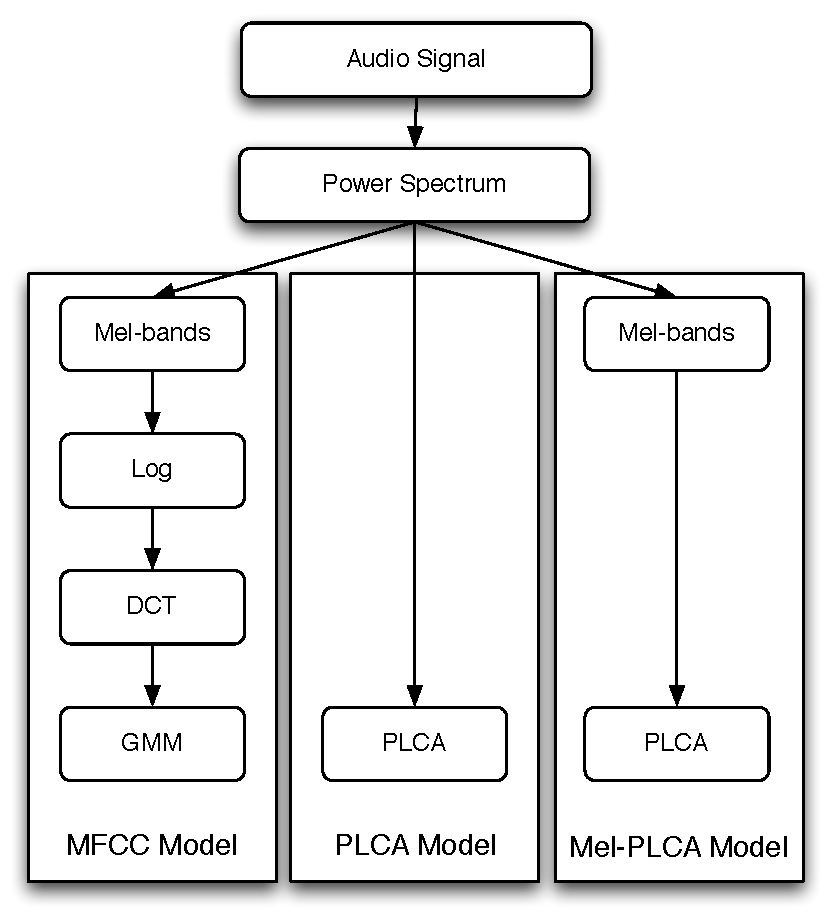
\includegraphics[width=0.5\textwidth]{images/models.pdf}
\caption{Overview of the different models}
\label{fig:models}
\end{figure}

\begin{figure}[!ht]
\begin{adjustwidth}{-12em}{-12em}
	\centering
        \begin{subfigure}[b]{0.15\textwidth}
                \centering
                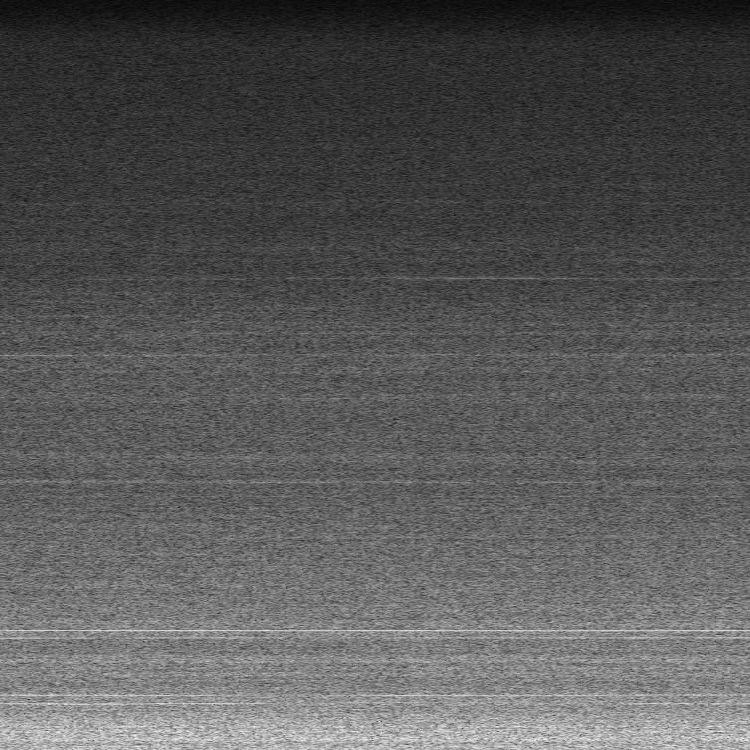
\includegraphics[width=\textwidth]{images/single/airplane.pdf}
                \caption*{Airplane}
        \end{subfigure}%
        \hspace{0.1pt}
        \begin{subfigure}[b]{0.15\textwidth}
                \centering
                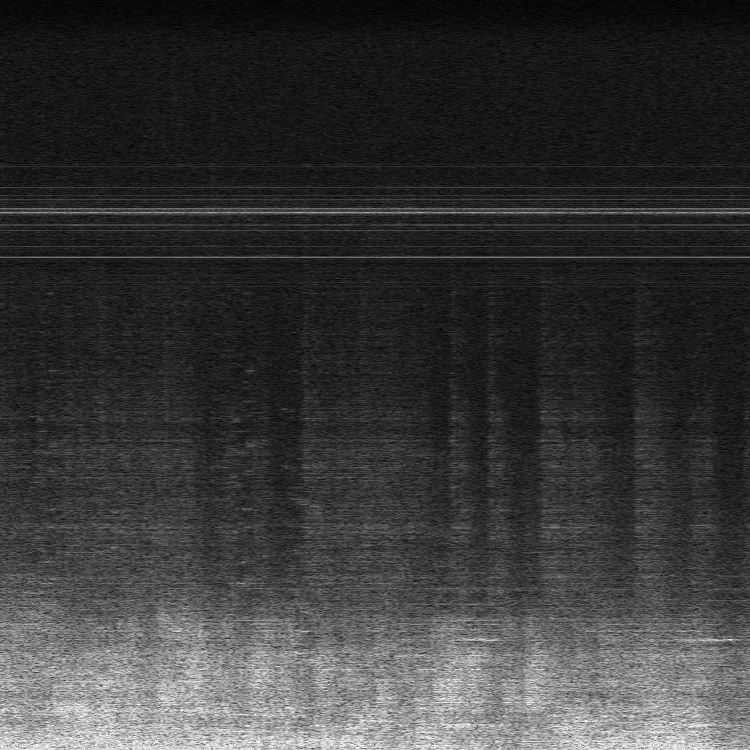
\includegraphics[width=\textwidth]{images/single/arcade.pdf}
                \caption*{Arcade}
        \end{subfigure}%
        \hspace{0.1pt}
        \begin{subfigure}[b]{0.15\textwidth}
                \centering
                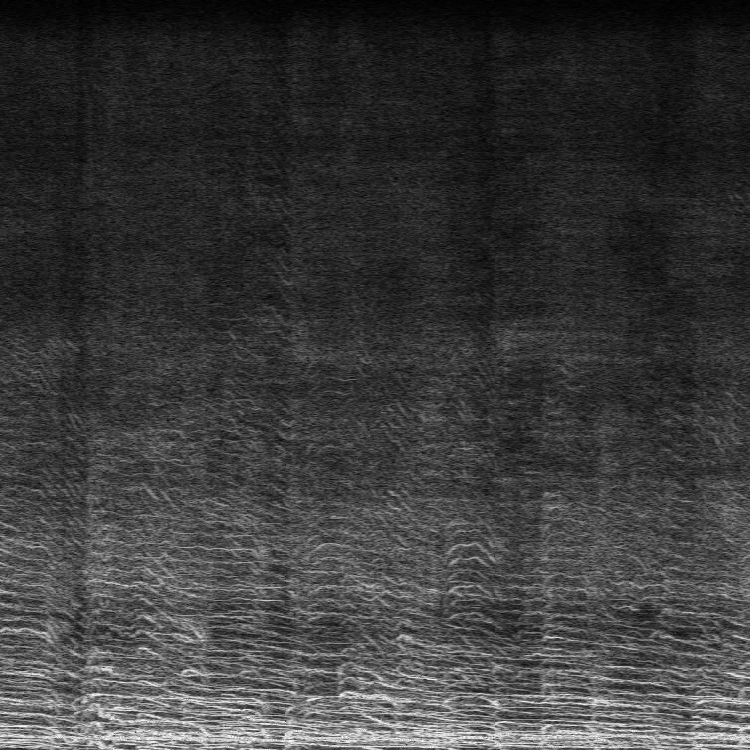
\includegraphics[width=\textwidth]{images/single/booing.pdf}
                \caption*{Booing}
        \end{subfigure}%        
        \hspace{0.1pt}
        \begin{subfigure}[b]{0.15\textwidth}
                \centering
                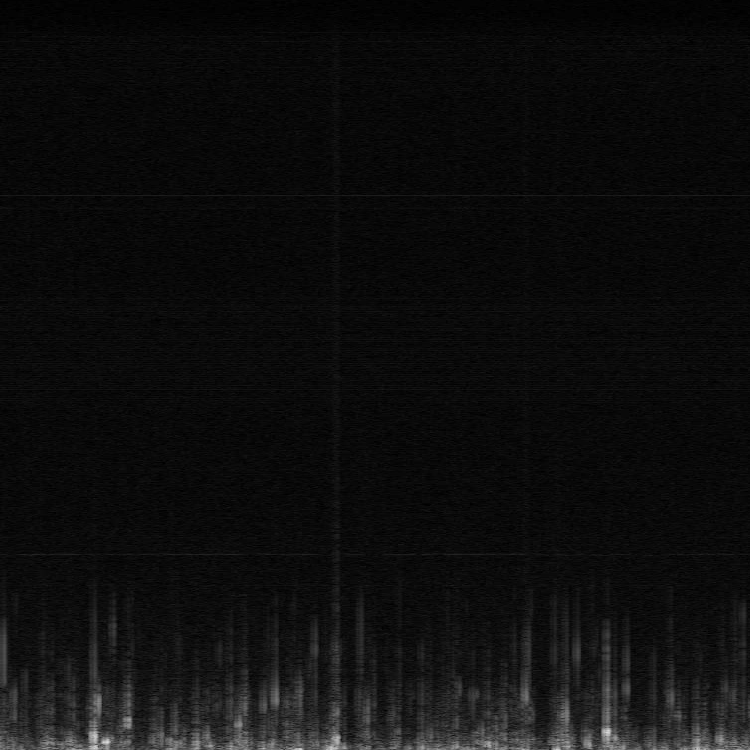
\includegraphics[width=\textwidth]{images/single/bubbles.pdf}
                \caption*{Bubbles}
        \end{subfigure}%
        \hspace{0.1pt}
        \begin{subfigure}[b]{0.15\textwidth}
                \centering
                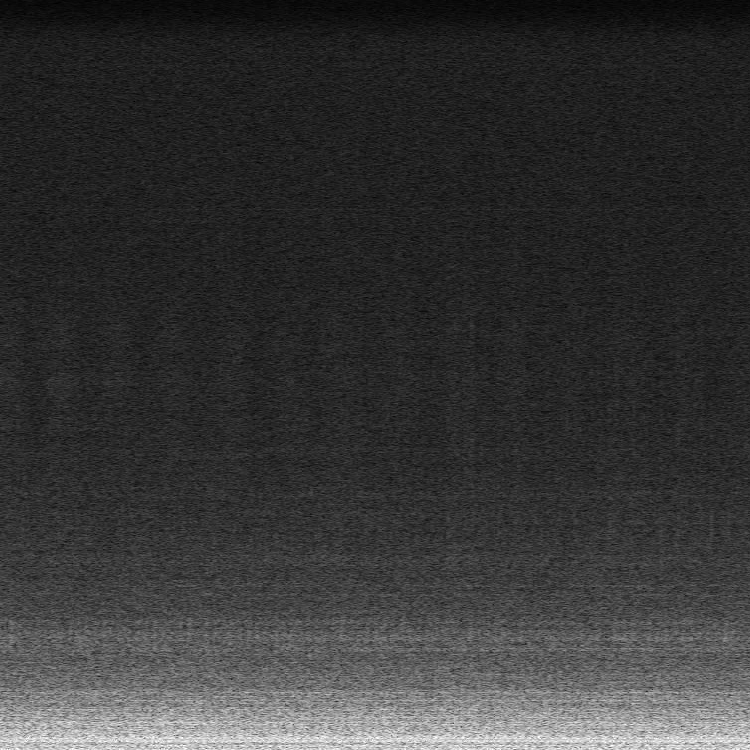
\includegraphics[width=\textwidth]{images/single/bus.pdf}
                \caption*{Bus}
        \end{subfigure}%
        \hspace{0.1pt}        
        \begin{subfigure}[b]{0.15\textwidth}
                \centering
                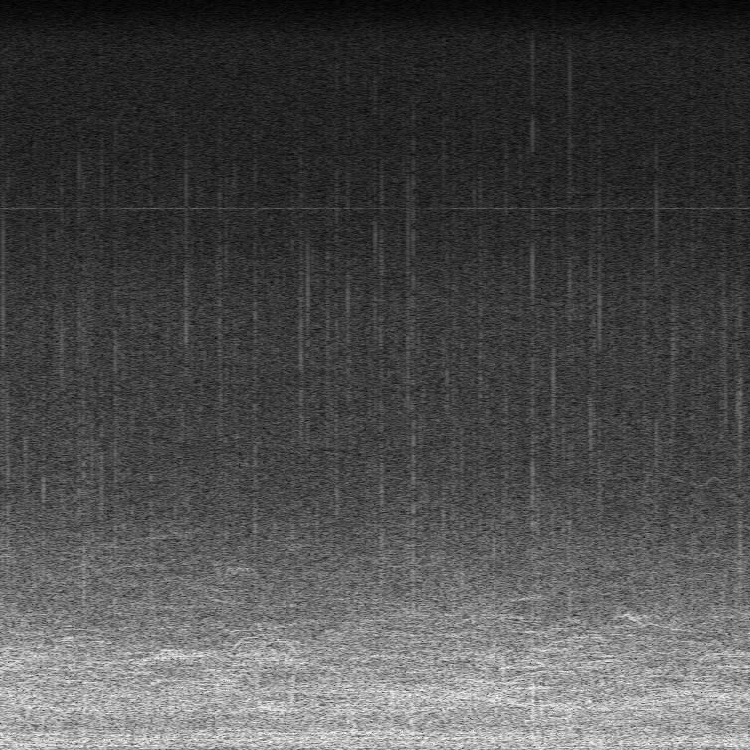
\includegraphics[width=\textwidth]{images/single/cheering.pdf}
                \caption*{Cheering}
        \end{subfigure}%

        \begin{subfigure}[b]{0.15\textwidth}
                \centering
                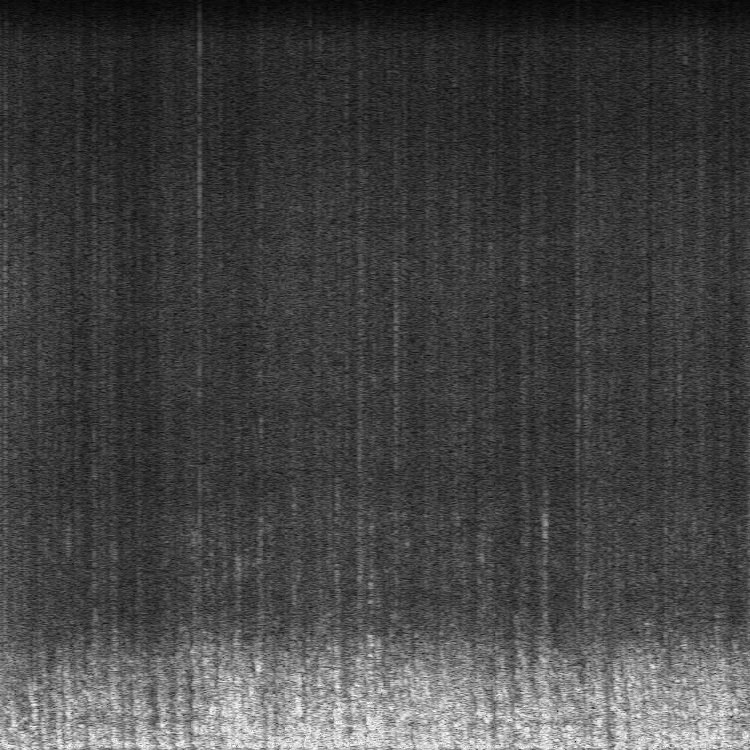
\includegraphics[width=\textwidth]{images/single/chickens.pdf}
                \caption*{Chickens}
        \end{subfigure}%      
        \hspace{0.1pt}                
        \begin{subfigure}[b]{0.15\textwidth}
                \centering
                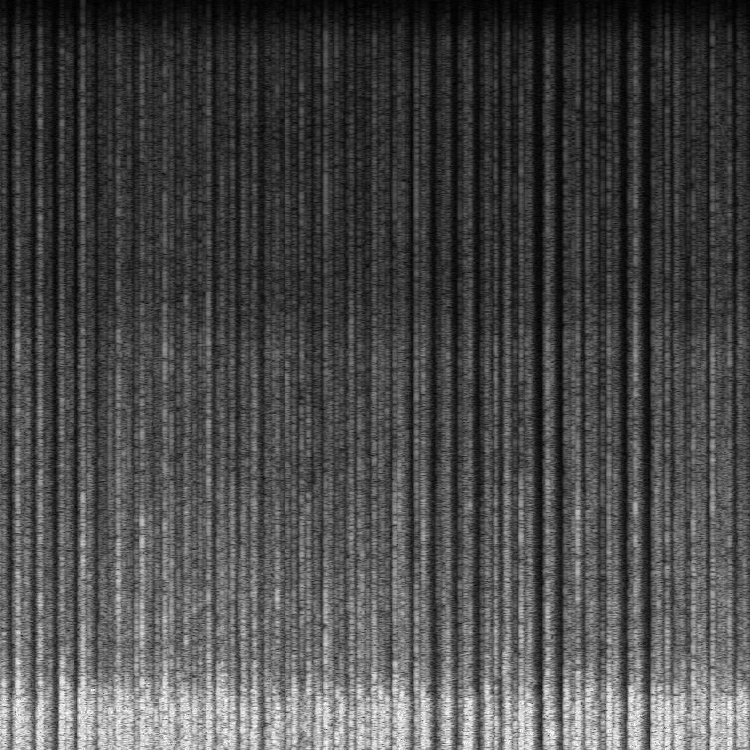
\includegraphics[width=\textwidth]{images/single/clapping.pdf}
                \caption*{Clapping}
        \end{subfigure}%
        \hspace{0.1pt}
        \begin{subfigure}[b]{0.15\textwidth}
                \centering
                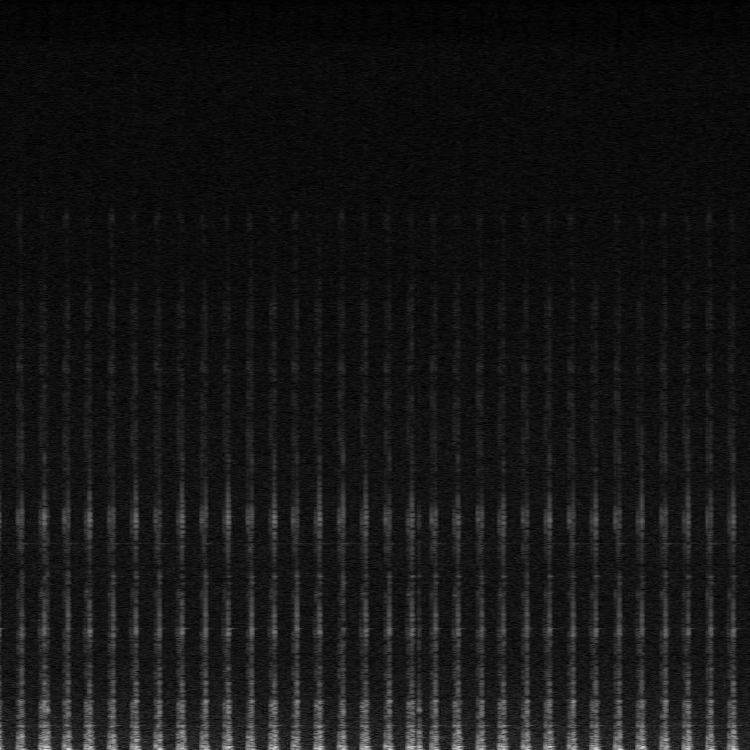
\includegraphics[width=\textwidth]{images/single/clock-ticking.pdf}
                \caption*{Clock Ticking}
        \end{subfigure}%
        \hspace{0.1pt}
        \begin{subfigure}[b]{0.15\textwidth}
                \centering
                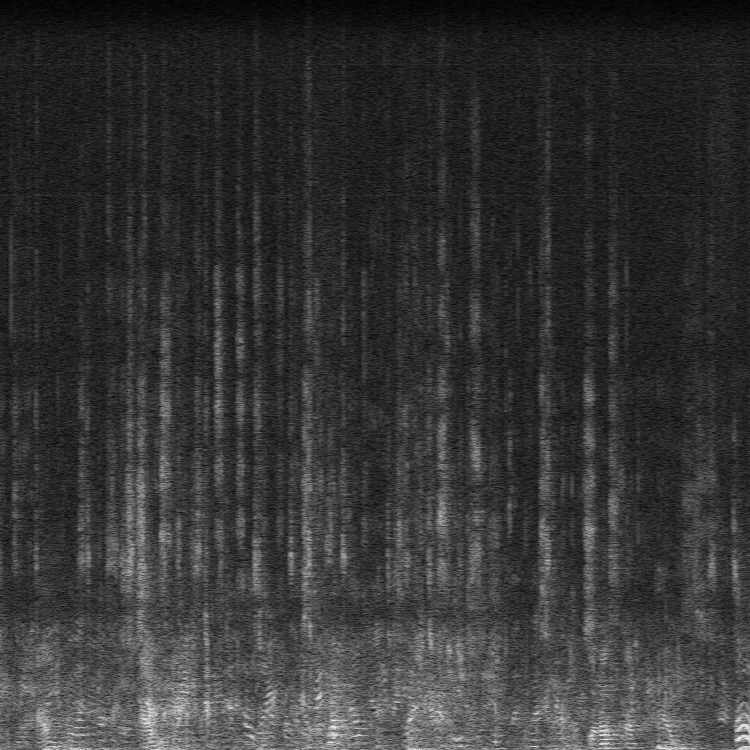
\includegraphics[width=\textwidth]{images/single/conversation.pdf}
                \caption*{Conversation}
        \end{subfigure}%
        \hspace{0.1pt}
        \begin{subfigure}[b]{0.15\textwidth}
                \centering
                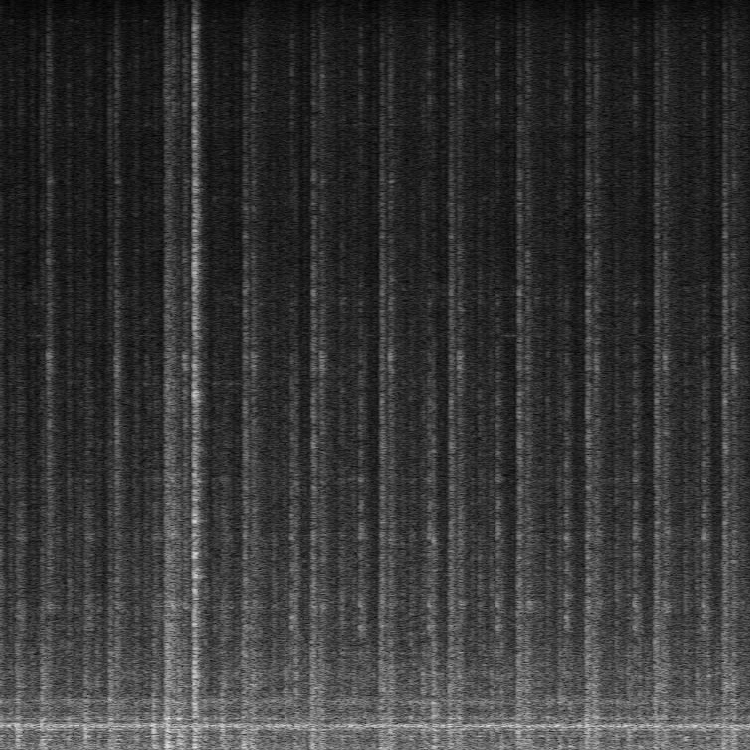
\includegraphics[width=\textwidth]{images/single/copier.pdf}
                \caption*{Copier}
        \end{subfigure}%        
        \hspace{0.1pt}
        \begin{subfigure}[b]{0.15\textwidth}
                \centering
                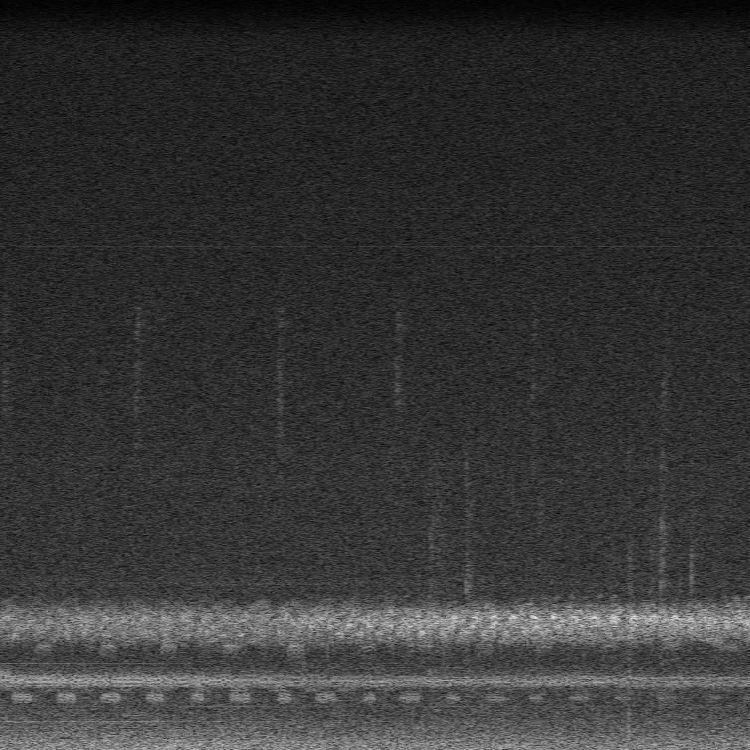
\includegraphics[width=\textwidth]{images/single/crickets.pdf}
                \caption*{Crickets}
        \end{subfigure}%

        \begin{subfigure}[b]{0.15\textwidth}
                \centering
                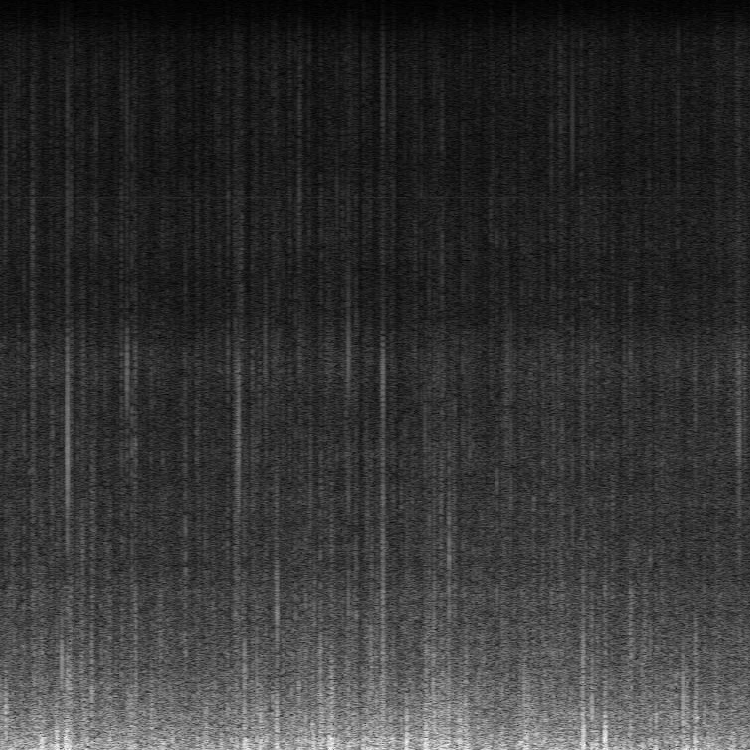
\includegraphics[width=\textwidth]{images/single/dirt-drive.pdf}
                \caption*{Dirt Drive}
        \end{subfigure}%
        \hspace{0.1pt}
        \begin{subfigure}[b]{0.15\textwidth}
                \centering
                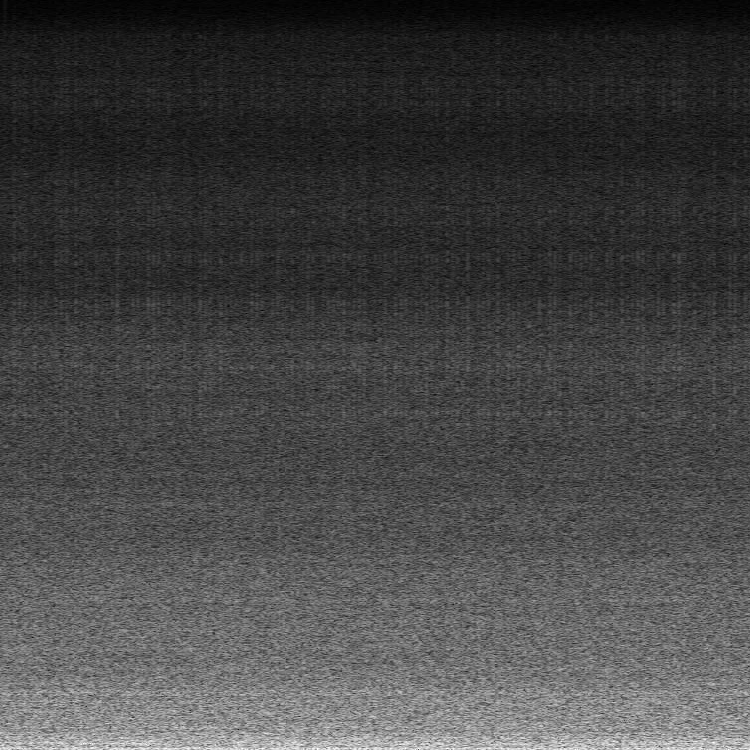
\includegraphics[width=\textwidth]{images/single/fan.pdf}
                \caption*{Fan}
        \end{subfigure}%
        \hspace{0.1pt}
        \begin{subfigure}[b]{0.15\textwidth}
                \centering
                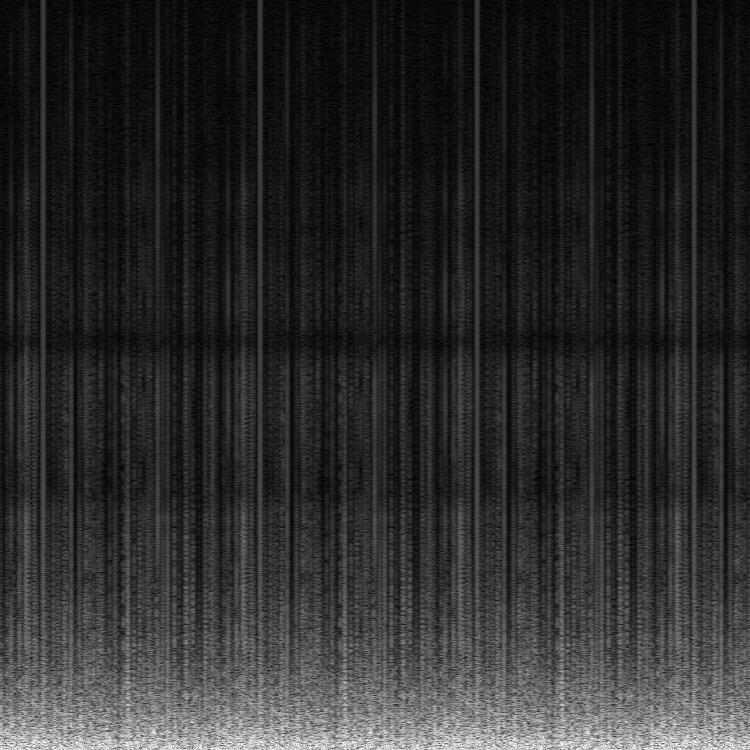
\includegraphics[width=\textwidth]{images/single/fire-gas.pdf}
                \caption*{Fire Gas}
        \end{subfigure}%       
        \hspace{0.1pt} 
        \begin{subfigure}[b]{0.15\textwidth}
                \centering
                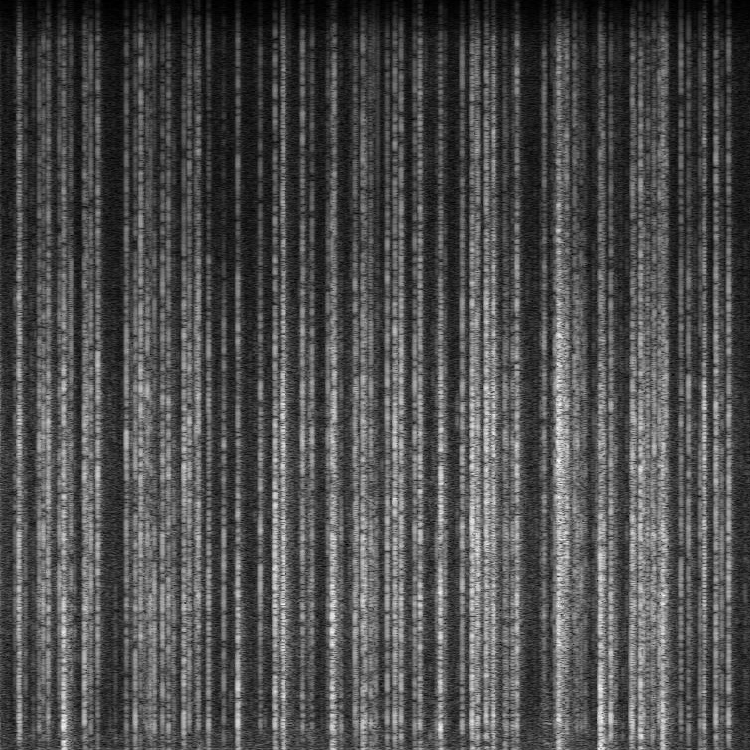
\includegraphics[width=\textwidth]{images/single/fire.pdf}
                \caption*{Fire}
        \end{subfigure}%
        \hspace{0.1pt}
        \begin{subfigure}[b]{0.15\textwidth}
                \centering
                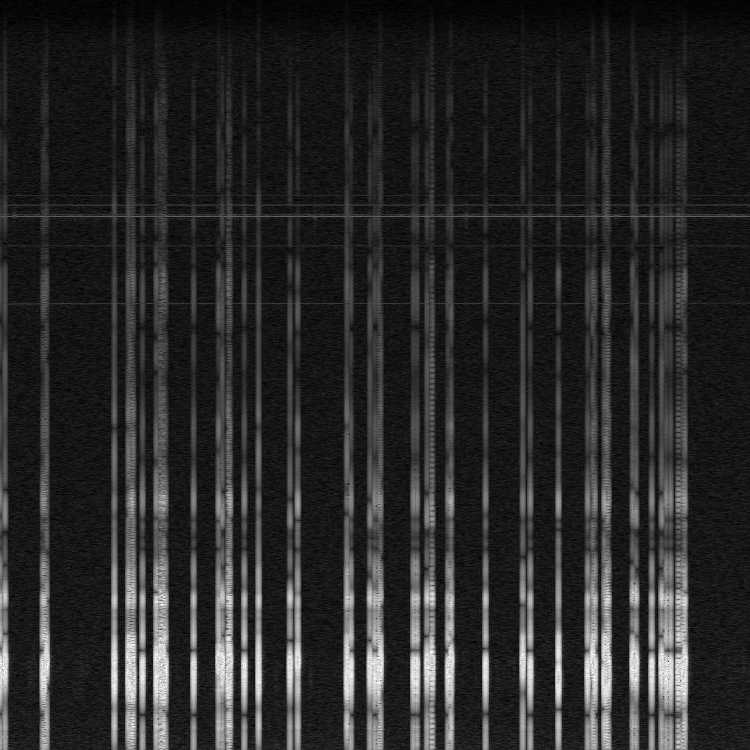
\includegraphics[width=\textwidth]{images/single/geiger.pdf}
                \caption*{Geiger}
        \end{subfigure}%
        \hspace{0.1pt}
        \begin{subfigure}[b]{0.15\textwidth}
                \centering
                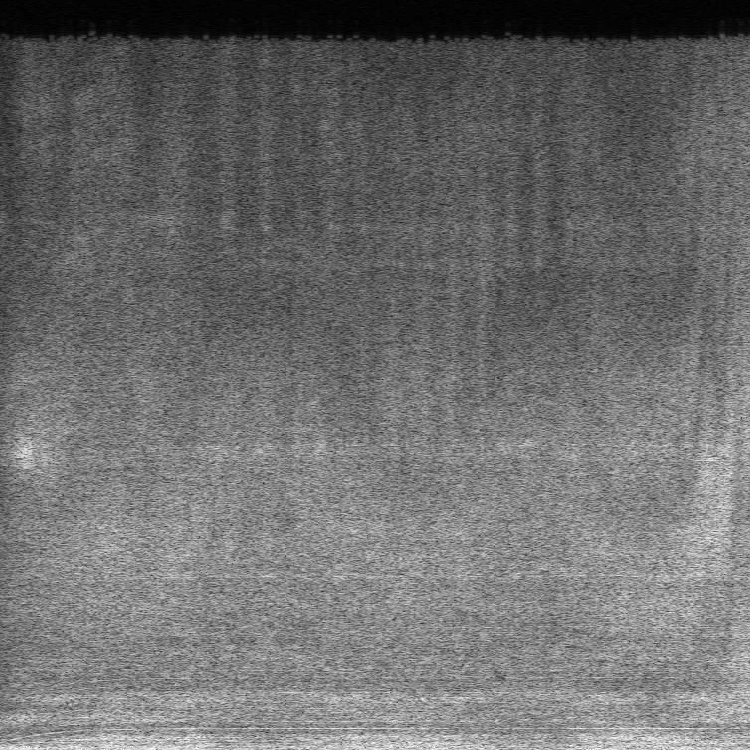
\includegraphics[width=\textwidth]{images/single/hair-dryer.pdf}
                \caption*{Hair Dryer}
        \end{subfigure}%

        \begin{subfigure}[b]{0.15\textwidth}
                \centering
                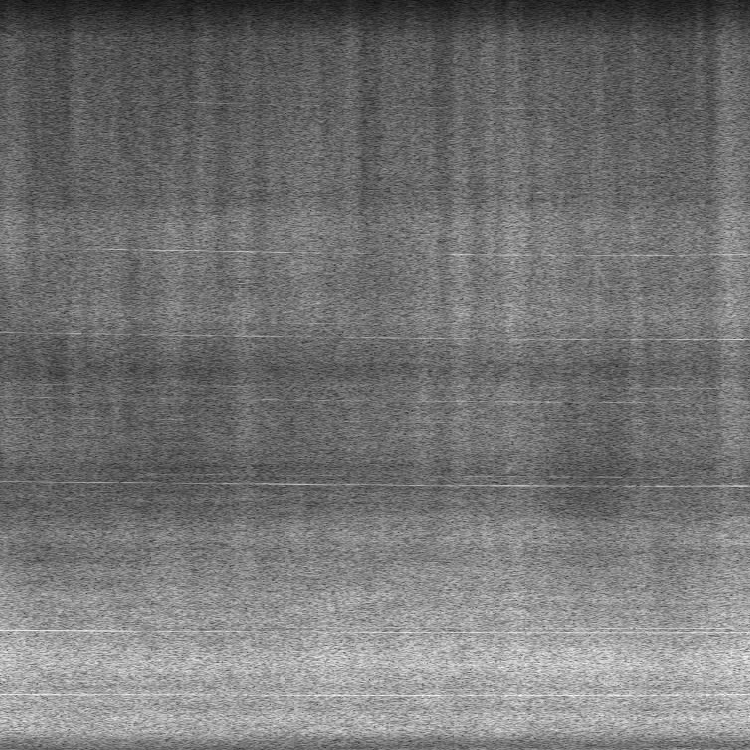
\includegraphics[width=\textwidth]{images/single/jet-engine.pdf}
                \caption*{Jet Engine}
        \end{subfigure}%        
        \hspace{0.1pt}
        \begin{subfigure}[b]{0.15\textwidth}
                \centering
                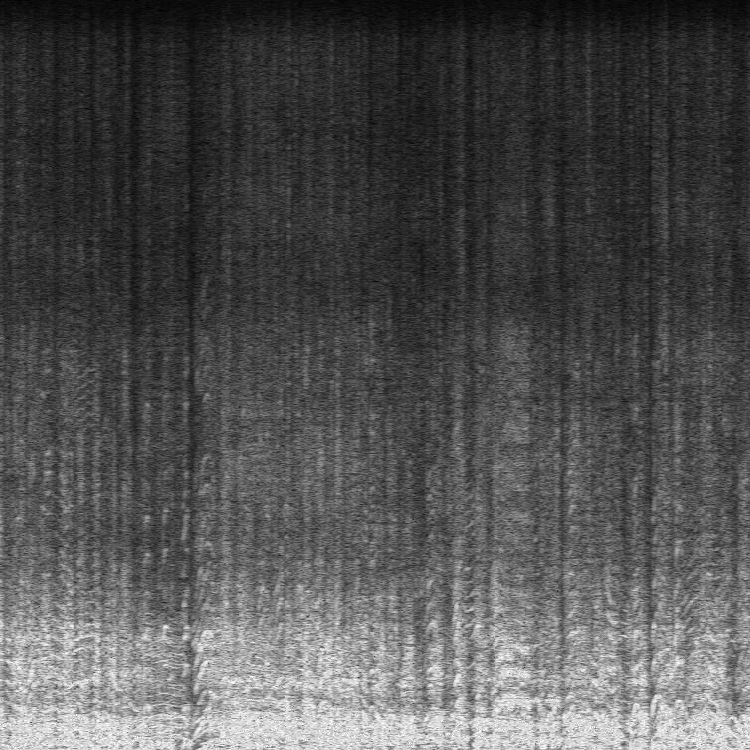
\includegraphics[width=\textwidth]{images/single/laughing-audience.pdf}
                \caption*{Laugh. Aud.}
        \end{subfigure}%
        \hspace{0.1pt}
        \begin{subfigure}[b]{0.15\textwidth}
                \centering
                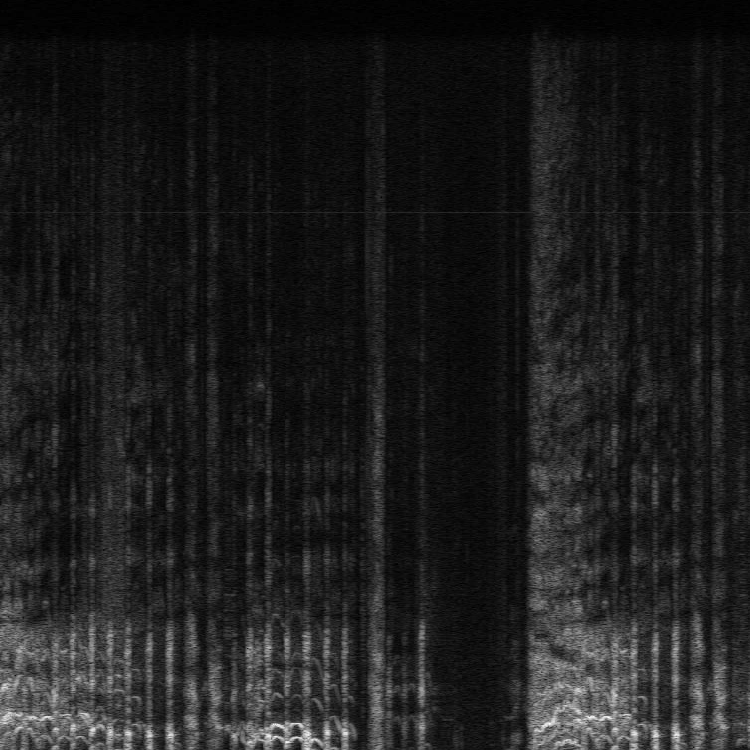
\includegraphics[width=\textwidth]{images/single/laughing-man.pdf}
                \caption*{Laugh. Man}
        \end{subfigure}%
        \hspace{0.1pt}
        \begin{subfigure}[b]{0.15\textwidth}
                \centering
                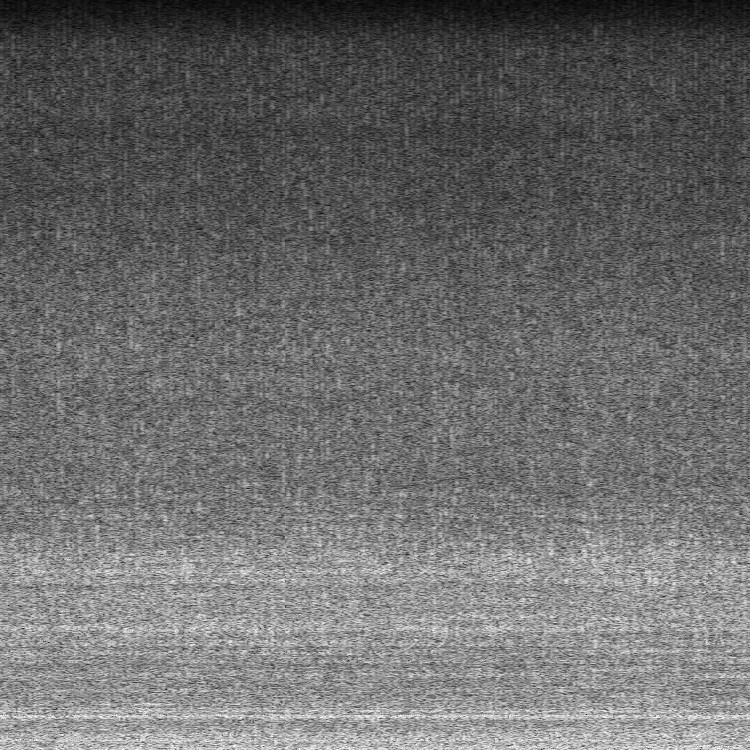
\includegraphics[width=\textwidth]{images/single/motor.pdf}
                \caption*{Motor}
        \end{subfigure}%
        \hspace{0.1pt}
        \begin{subfigure}[b]{0.15\textwidth}
                \centering
                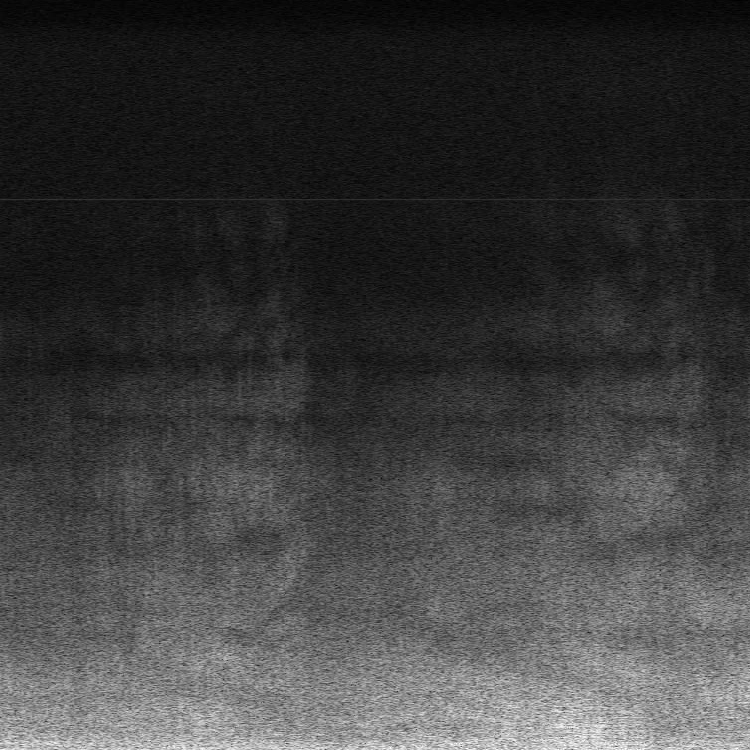
\includegraphics[width=\textwidth]{images/single/race.pdf}
                \caption*{Race}
        \end{subfigure}%        
        \hspace{0.1pt}
        \begin{subfigure}[b]{0.15\textwidth}
                \centering
                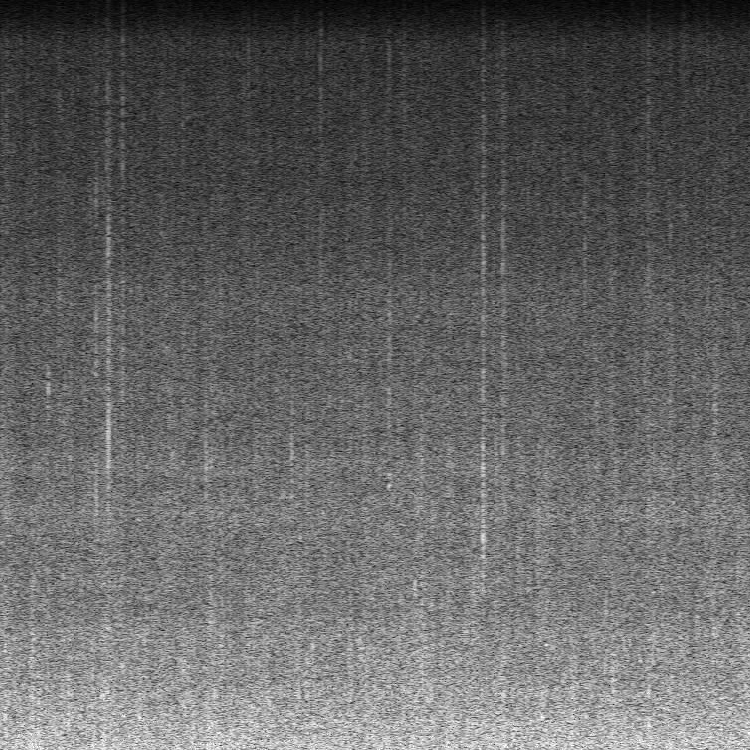
\includegraphics[width=\textwidth]{images/single/rain.pdf}
                \caption*{Rain}
        \end{subfigure}%

        \begin{subfigure}[b]{0.15\textwidth}
                \centering
                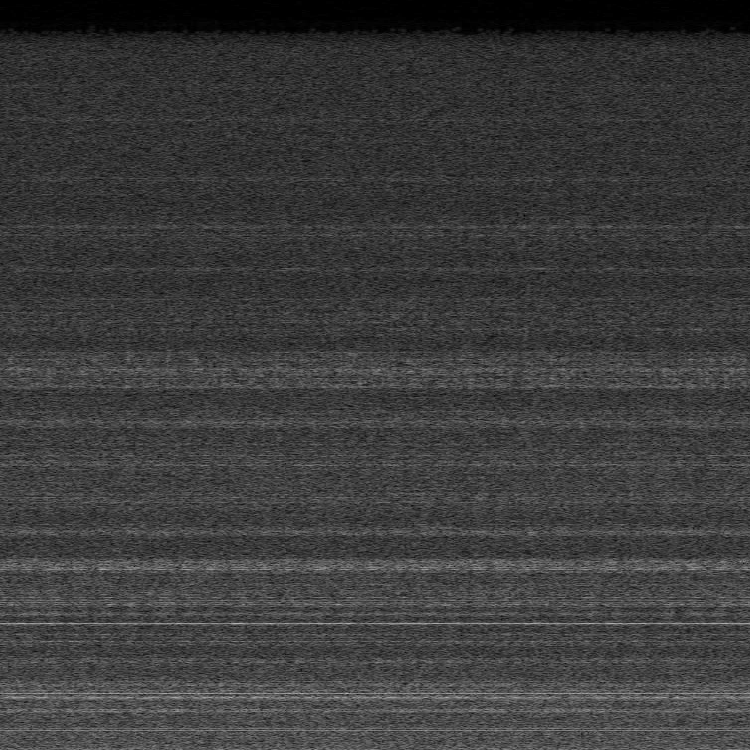
\includegraphics[width=\textwidth]{images/single/refridgerator.pdf}
                \caption*{Refridge.}
        \end{subfigure}%
        \hspace{0.1pt}
        \begin{subfigure}[b]{0.15\textwidth}
                \centering
                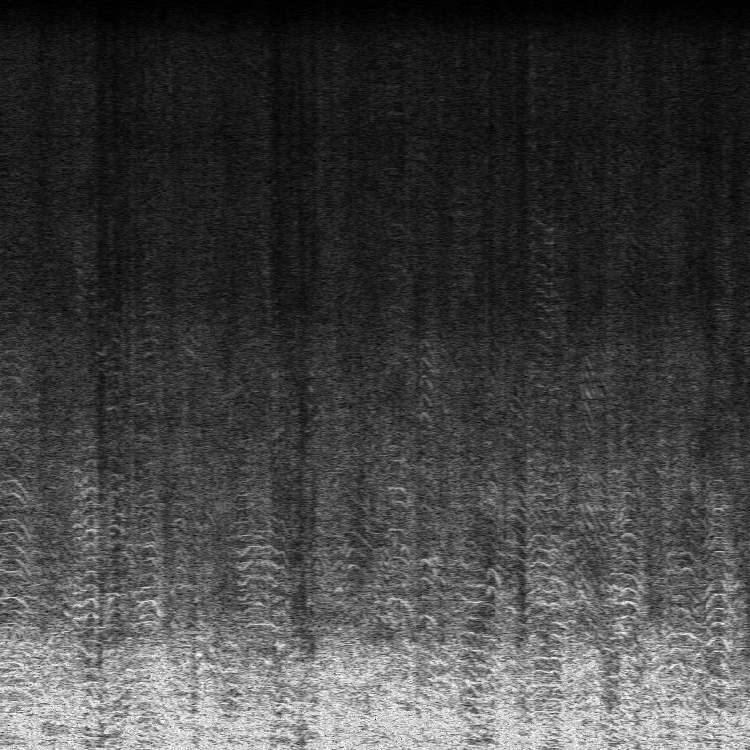
\includegraphics[width=\textwidth]{images/single/shouting.pdf}
                \caption*{Shouting}
        \end{subfigure}%
        \hspace{0.1pt}
        \begin{subfigure}[b]{0.15\textwidth}
                \centering
                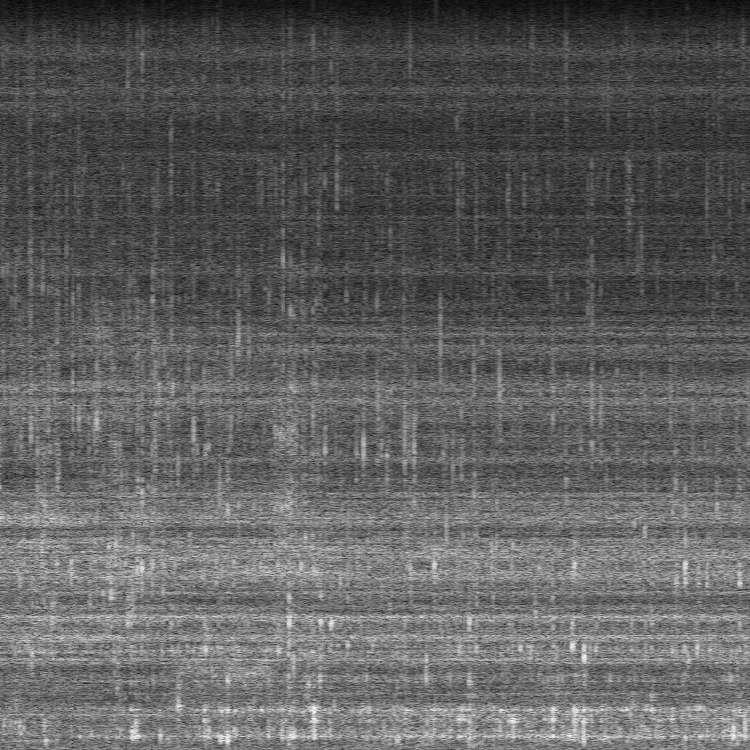
\includegraphics[width=\textwidth]{images/single/sink.pdf}
                \caption*{Sink}
        \end{subfigure}%        
        \hspace{0.1pt}
        \begin{subfigure}[b]{0.15\textwidth}
                \centering
                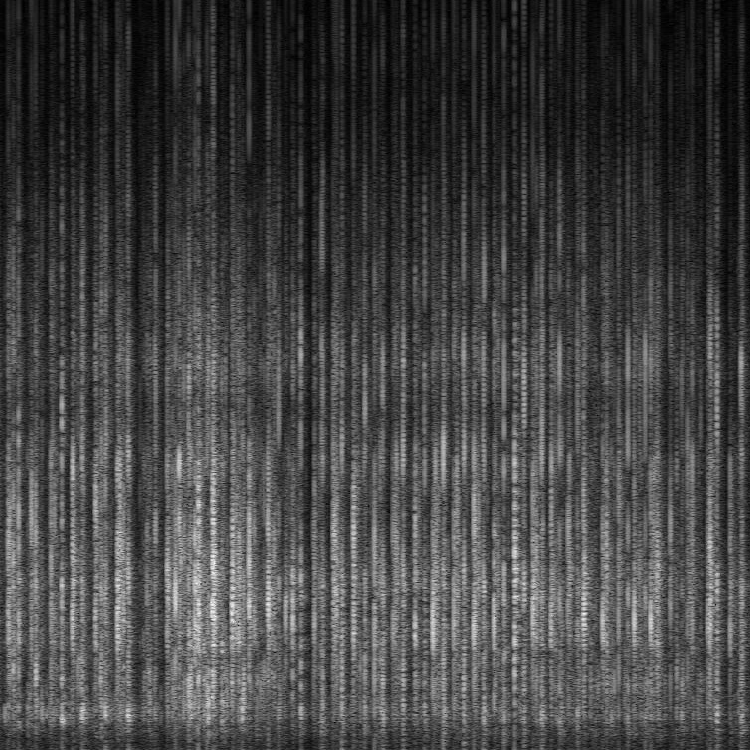
\includegraphics[width=\textwidth]{images/single/spray-can.pdf}
                \caption*{Spray.}
        \end{subfigure}%  
        \hspace{0.1pt}        
        \begin{subfigure}[b]{0.15\textwidth}
                \centering
                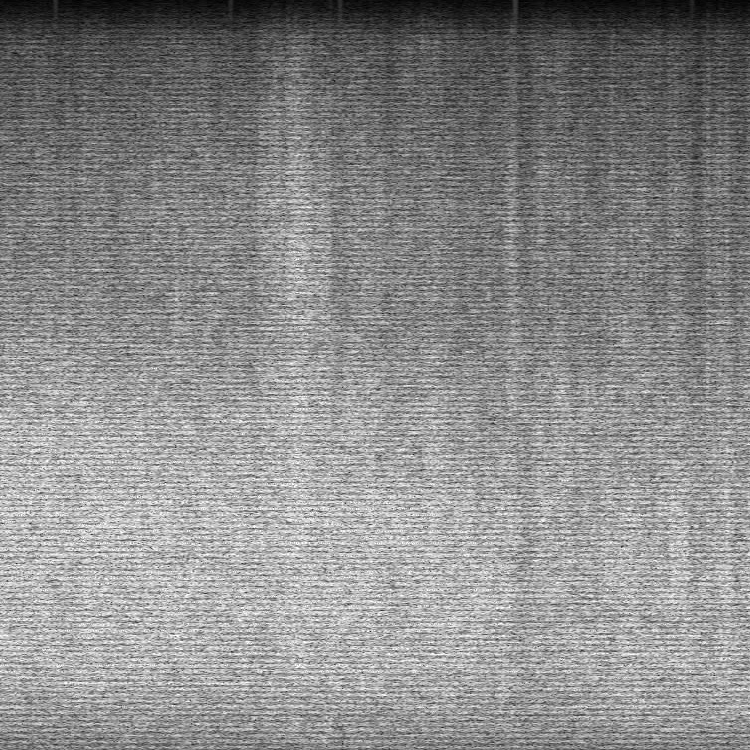
\includegraphics[width=\textwidth]{images/single/steam.pdf}
                \caption*{Steam}
        \end{subfigure}%
        \hspace{0.1pt}
        \begin{subfigure}[b]{0.15\textwidth}
                \centering
                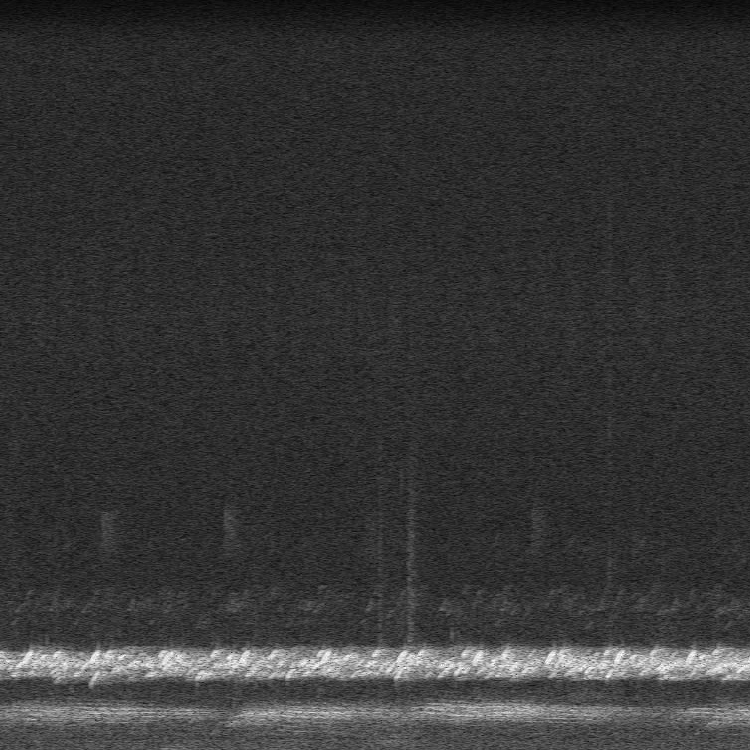
\includegraphics[width=\textwidth]{images/single/swamp.pdf}
                \caption*{Swamp}
        \end{subfigure}%
   
        \begin{subfigure}[b]{0.15\textwidth}
                \centering
                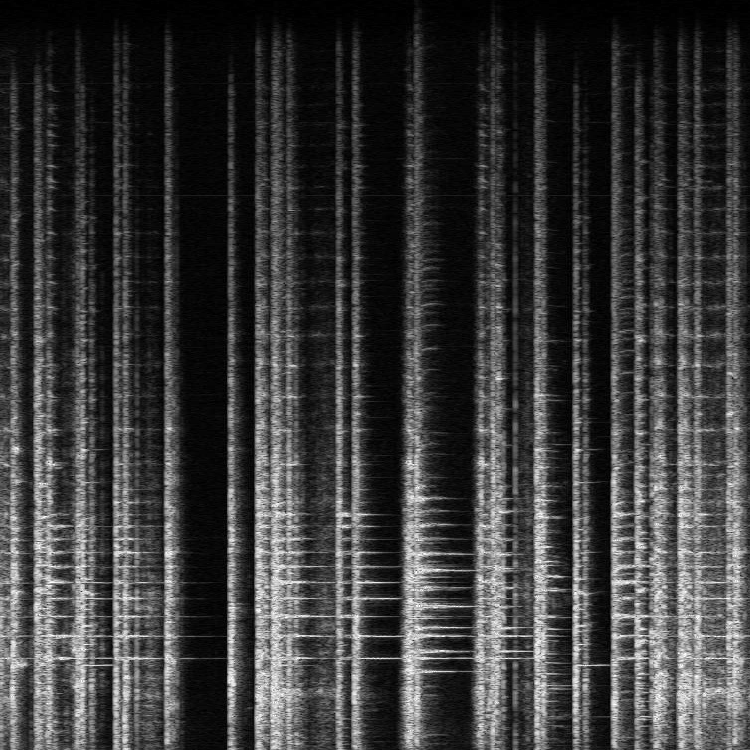
\includegraphics[width=\textwidth]{images/single/sword.pdf}
                \caption*{Sword}
        \end{subfigure}%
        \hspace{0.1pt}
        \begin{subfigure}[b]{0.15\textwidth}
                \centering
                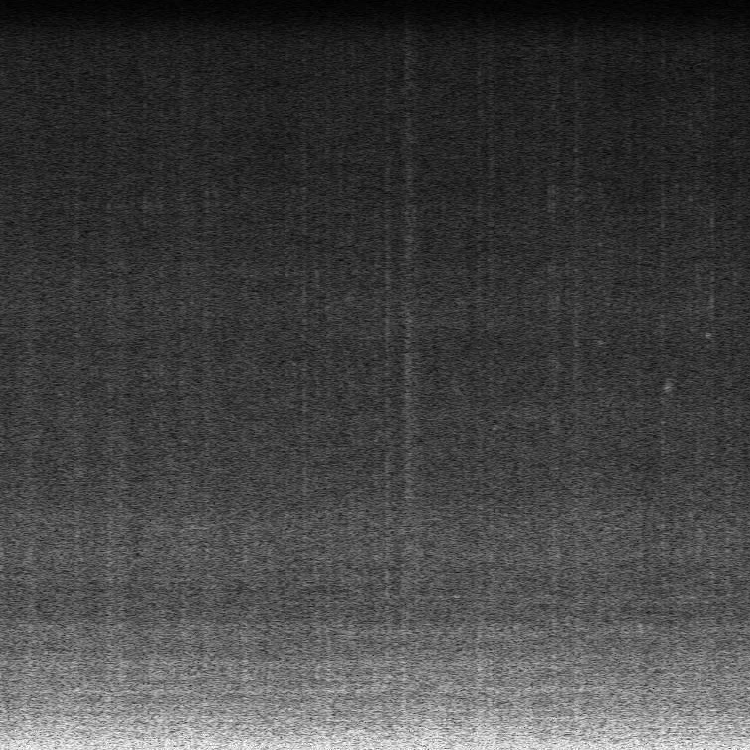
\includegraphics[width=\textwidth]{images/single/train.pdf}
                \caption*{Train}
        \end{subfigure}%
        \hspace{0.1pt}
        \begin{subfigure}[b]{0.15\textwidth}
                \centering
                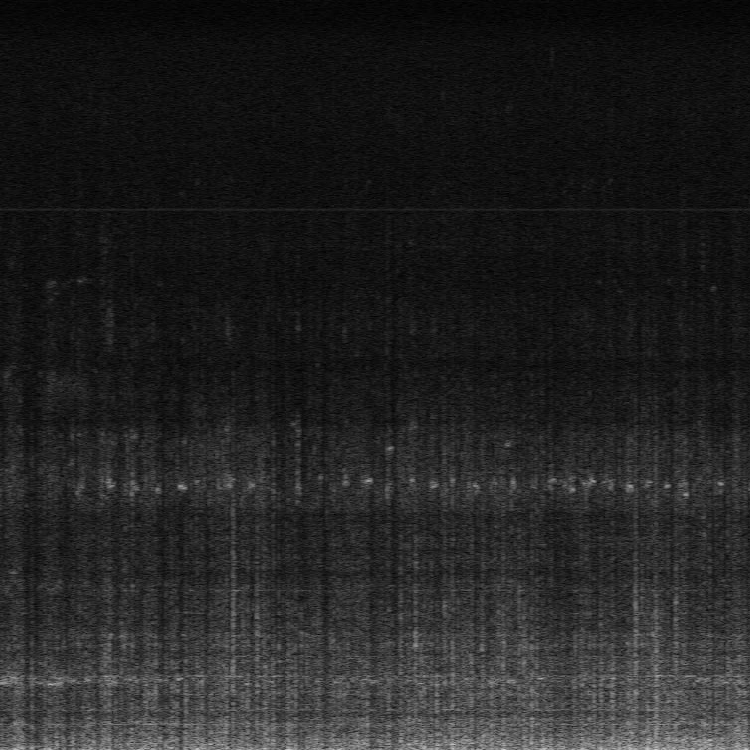
\includegraphics[width=\textwidth]{images/single/treads.pdf}
                \caption*{Treads}
        \end{subfigure}%        
        \hspace{0.1pt}
        \begin{subfigure}[b]{0.15\textwidth}
                \centering
                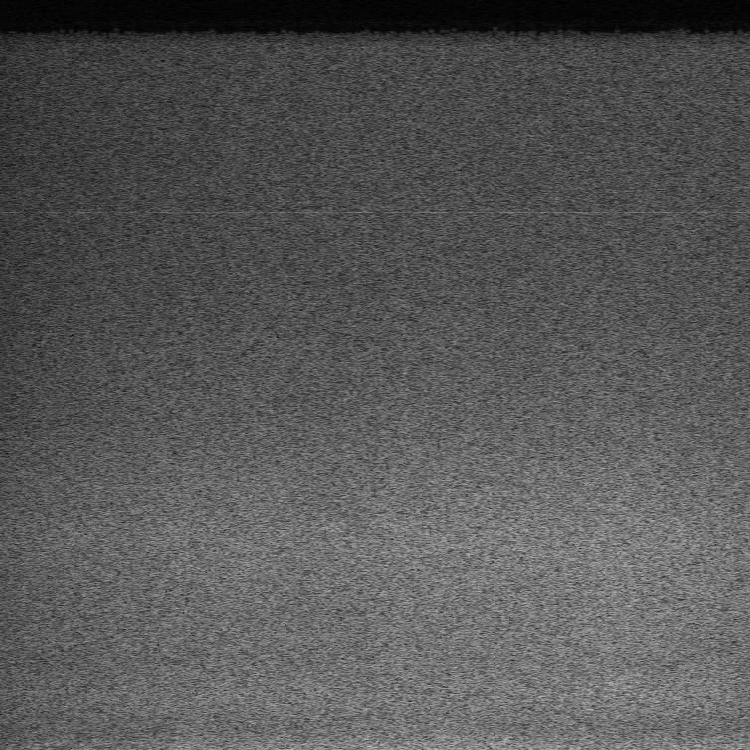
\includegraphics[width=\textwidth]{images/single/trees.pdf}
                \caption*{Trees}
        \end{subfigure}%  
        \hspace{0.1pt}
        \begin{subfigure}[b]{0.15\textwidth}
                \centering
                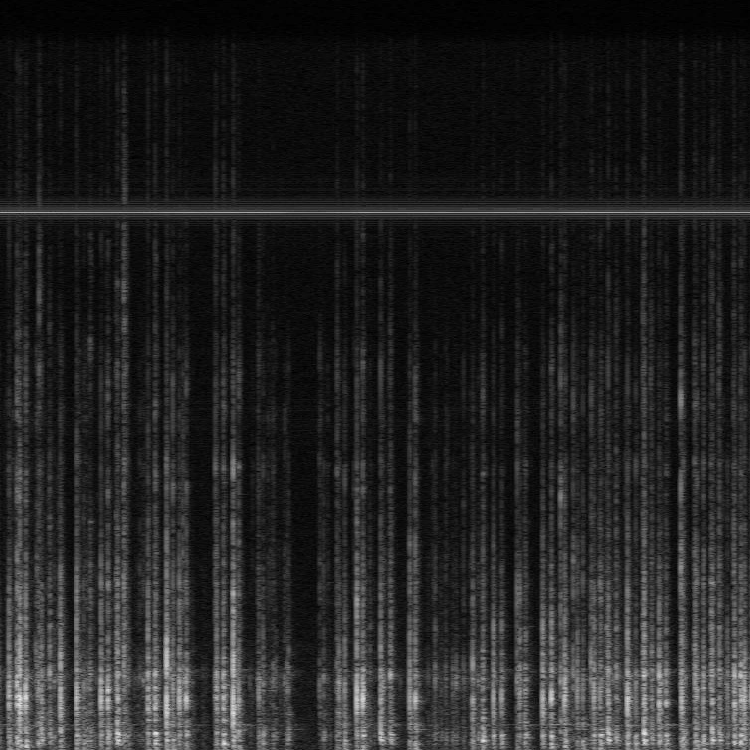
\includegraphics[width=\textwidth]{images/single/typing.pdf}
                \caption*{Typing}
        \end{subfigure}%
        \hspace{0.1pt}     
        \begin{subfigure}[b]{0.15\textwidth}
                \centering
                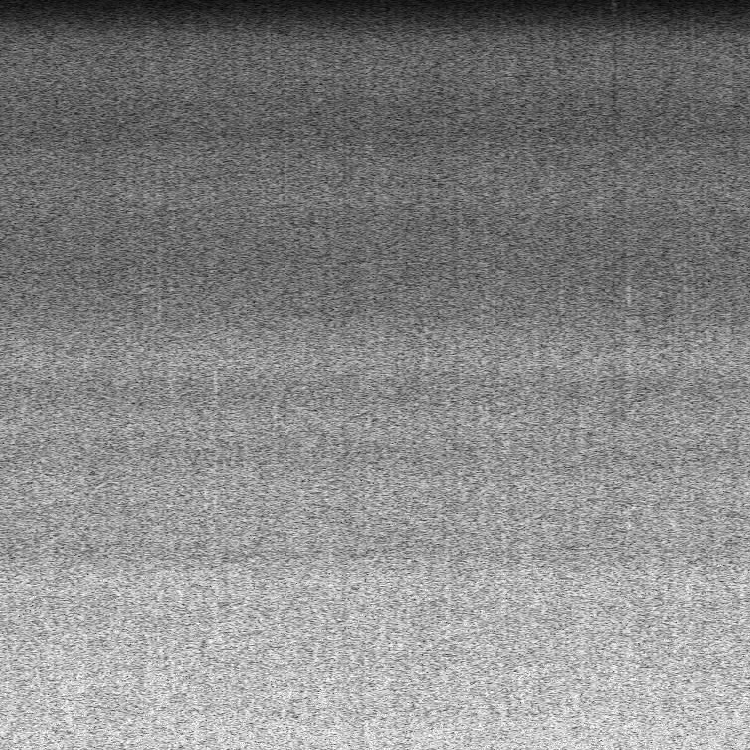
\includegraphics[width=\textwidth]{images/single/waterfall.pdf}
                \caption*{Waterfall}
        \end{subfigure}%
	\hspace{0.1pt}
        \begin{subfigure}[b]{0.15\textwidth}
                \centering
                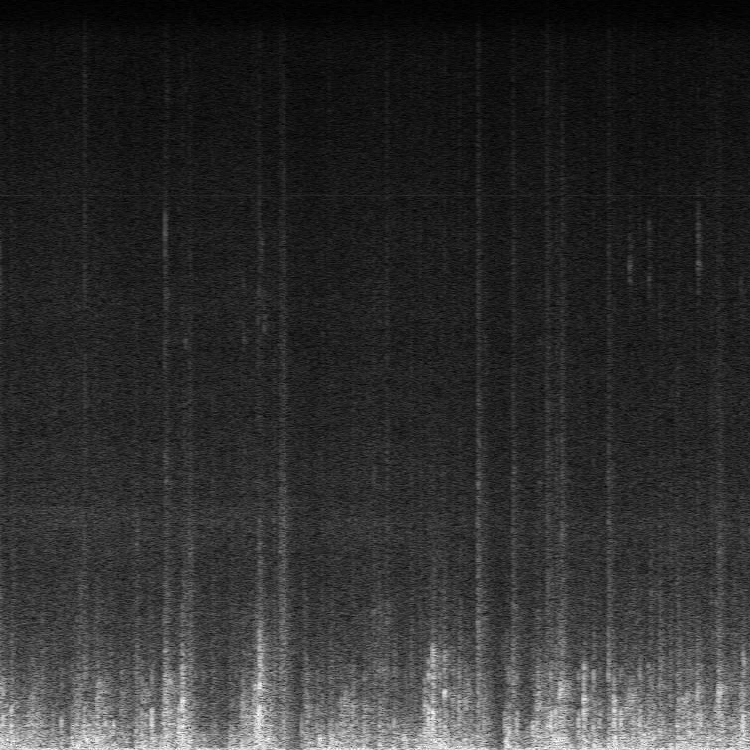
\includegraphics[width=\textwidth]{images/single/wooden-gears.pdf}
                \caption*{Wood. Gears}
        \end{subfigure}%        
\end{adjustwidth}
        \caption{Spectrum describing the frequencies (y-axis) over time (x-axis) of our 37 different classes.  White corresponds to higher values.}
\end{figure}

\subsection{Experiments}

\paragraph{Experiment 1}
We train one classifier for each of our possible acoustic event classes, thus building a set of 37 classifiers for experiment 1.

\paragraph{Experiment 2}
We also determined whether the MFCC and PLCA models were able to correctly classify the trained class in the presence of an untrained class (noise).  As we have 37 classes, this equates to 36 possible mixtures for each class, where each of the 36 classes are trained in isolation, and tested in a mixture of a 37th untrained class.  In order to create the $37*36 = 1332$ possible mixtures, we used balanced mixing.  For this experiment, this means each class is actually represented with 36 possible examples (36 possible mixtures for each class).  

\paragraph{Experiment 3}
Finally, we added the 37th un-trained class to the set of possible classifiers in order to see if both classes could be correctly classified when presented as an acoustic mixture.  This means we tested on $37\choose2$ $= 666$ possible mixtures and sought to find out whether the MFCC and PLCA models were capable of classifying either or both of the mixed acoustic classes, even though they were presented as a single acoustic stream.

\subsection{Validation and Reporting}
\label{sec:ROC}
We performed k-fold cross-validation using 10-folds.  With 10 seconds per class (370 seconds total), this equates to 1 second folds per class where training occurs on 9 seconds of material per class, and testing occurs on 1 second of material per example. The results of all folds were then averaged together to produce a single estimation.

In order to assess the estimated results, we made use of a standard technique in describing classification performance, the Receiver Operator Characteristic (ROC) curve.  ROC analysis describes ground truth classes as true and false and the predicted measures as positive and negative for a binary classifier.  The ROC curve then measures the accuracy of the classifier in separating the actual true class from the non-classes by relating the sensitivity, or the \textit{true positive rate}, against 1$-$specificity, or the \textit{false positive rate}.   In order to build the curve for a continuous classifier, the classifier's response must be converted to a set of binary classifiers by using equally spaced thresholds.  Using equally spaced thresholds will tell us the classifiers performance across a range of possible thresholds.   We do this since we do not know what the ``perfect'' threshold of our classifier is but are still interested in its performance.  We calculate the true positive rate of a bin $i$ as: 

\begin{equationb}
\text{TPR}_i = \frac{\text{TP}}{\text{TP} + \text{FN}}
\end{equationb}

and the false positive rate as: 

\begin{equationb}
\text{FPR}_i = \frac{\text{FP}}{\text{TN} + \text{FP}}
\end{equationb}

The resulting $(x,y)$ points relating the false positive rate to the true positive rate are plotted for each classifier.

A perfect score is denoted by 100\% sensitivity (no false negatives) and 100\% specificity (no false positives) and corresponds to a point in the top-left corner, (0,1).  A classifier that performs at chance lies along the diagonal going from the bottom-left to the top-right corner.  

The area under the ROC curve (AUC) neatly summarizes the performance of the curve with 1.0 being a perfect score, and 0.5 being a classifier that performs at chance.  We can also understand the AUC as the probability of classifying a randomly chosen positive instance with higher likelihood than a negative one.

\section{Results}

\subsection{Experiment 1: Classifying isolated acoustic events}

We tested the performance of a single event class in isolation.  The performance of the MFCC and PLCA models as determined by the ROC analysis are all excellent, with an AUC of within 0.001 of perfect discrimination.  Each of these methods have classified fragments of a longer sound source and were able to extrapolate to the last second of untrained sound with high accuracy.  These results suggest that all three computational methods are suitable for representing acoustic scenes when they do not need to be segregated.

%performance during sound classification of 37 classes 
%	- handle different amplitudes
%	- microphone dynamics? 
%	- similar classes? 

%As we'd expect, the performance of both the MFCC and PLCA models perform with a perfect AUC.  

%GMM-MFCC: 98.4\%, PLCA-1c: 78.1\%

\subsection{Experiment 2: Classifying acoustic events in the presence of noise}

\begin{figure}
\centering
	\begin{subfigure}[b]{0.48\textwidth}
		\centering
		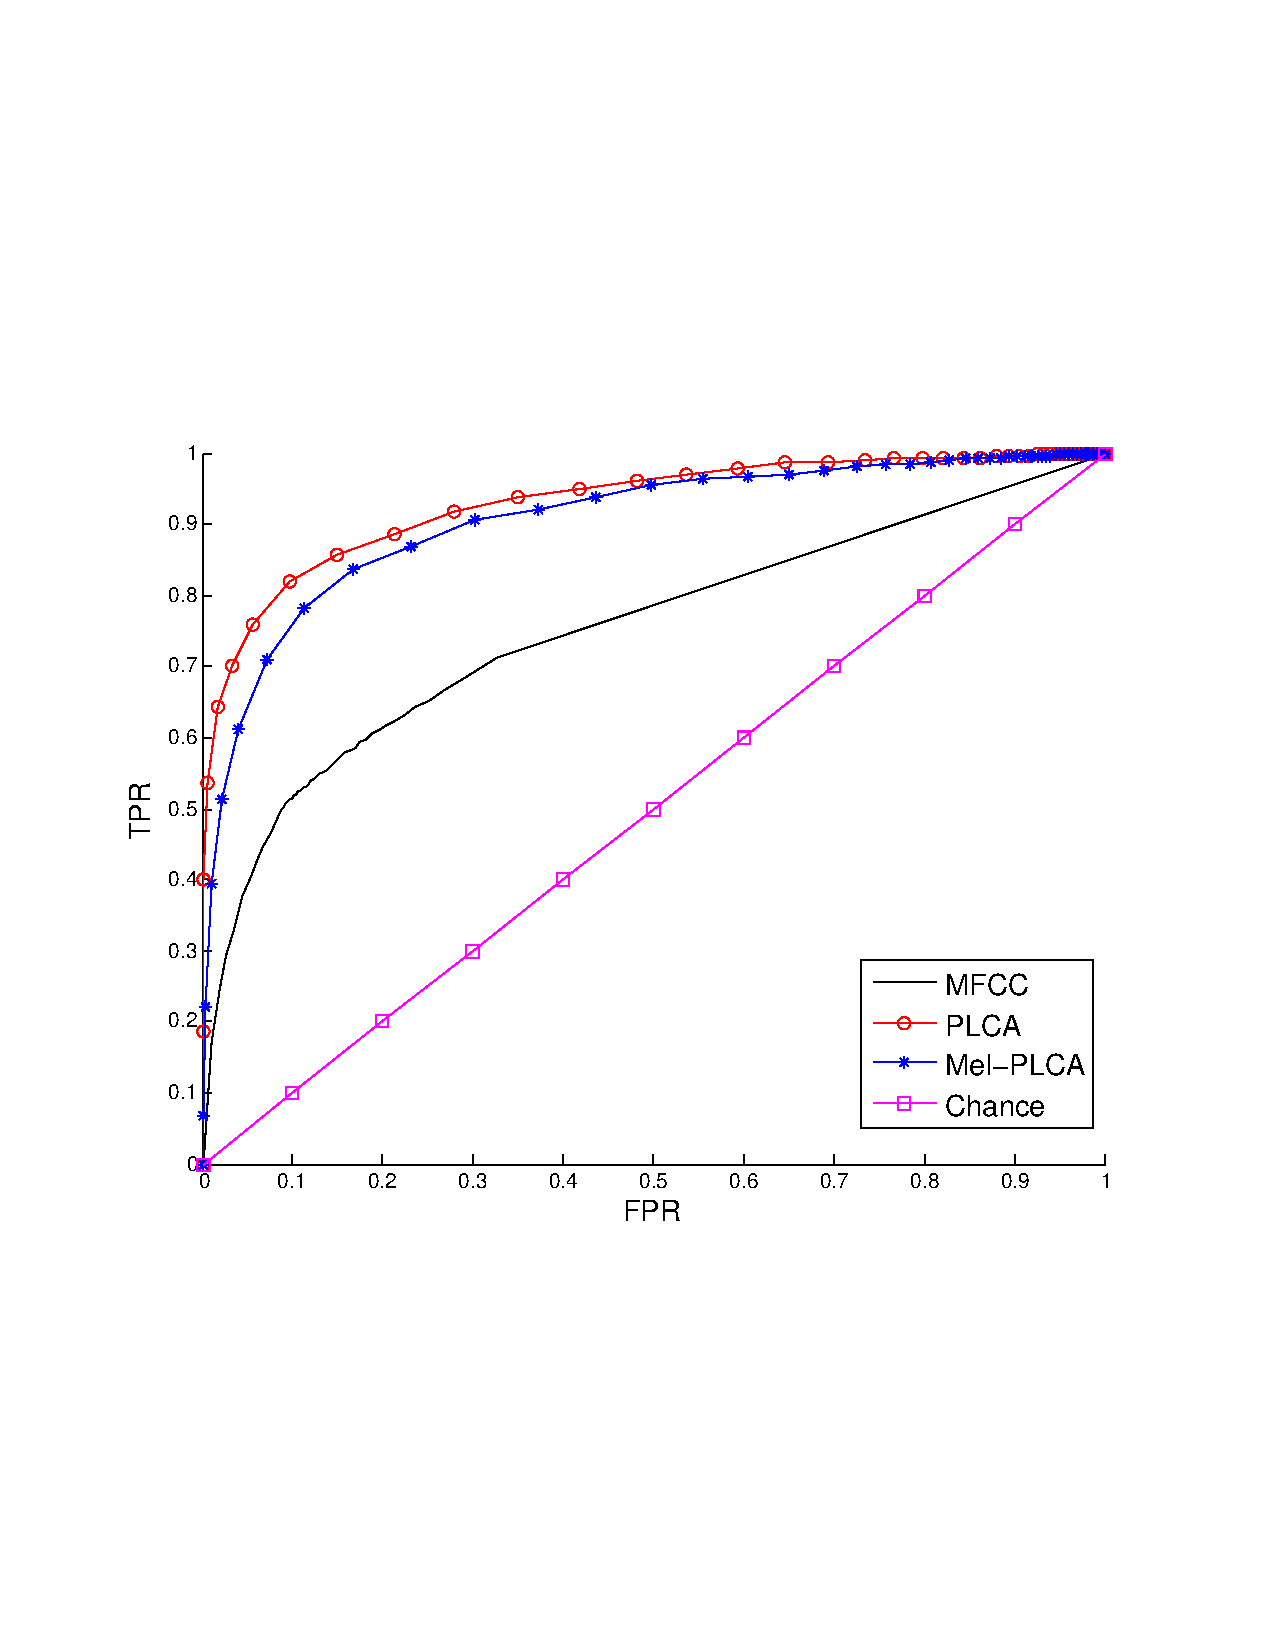
\includegraphics[width=0.99\textwidth]{images/unknown-mixture-roc-results.pdf}
		\caption{Experiment 2: Classification masked by noise.}
		\label{fig:unknown-mixture-roc-results}
	\end{subfigure}%
        ~ %add desired spacing between images, e. g. ~, \quad, \qquad etc.
          %(or a blank line to force the subfigure onto a new line)
      \begin{subfigure}[b]{0.48\textwidth}
      		\centering
		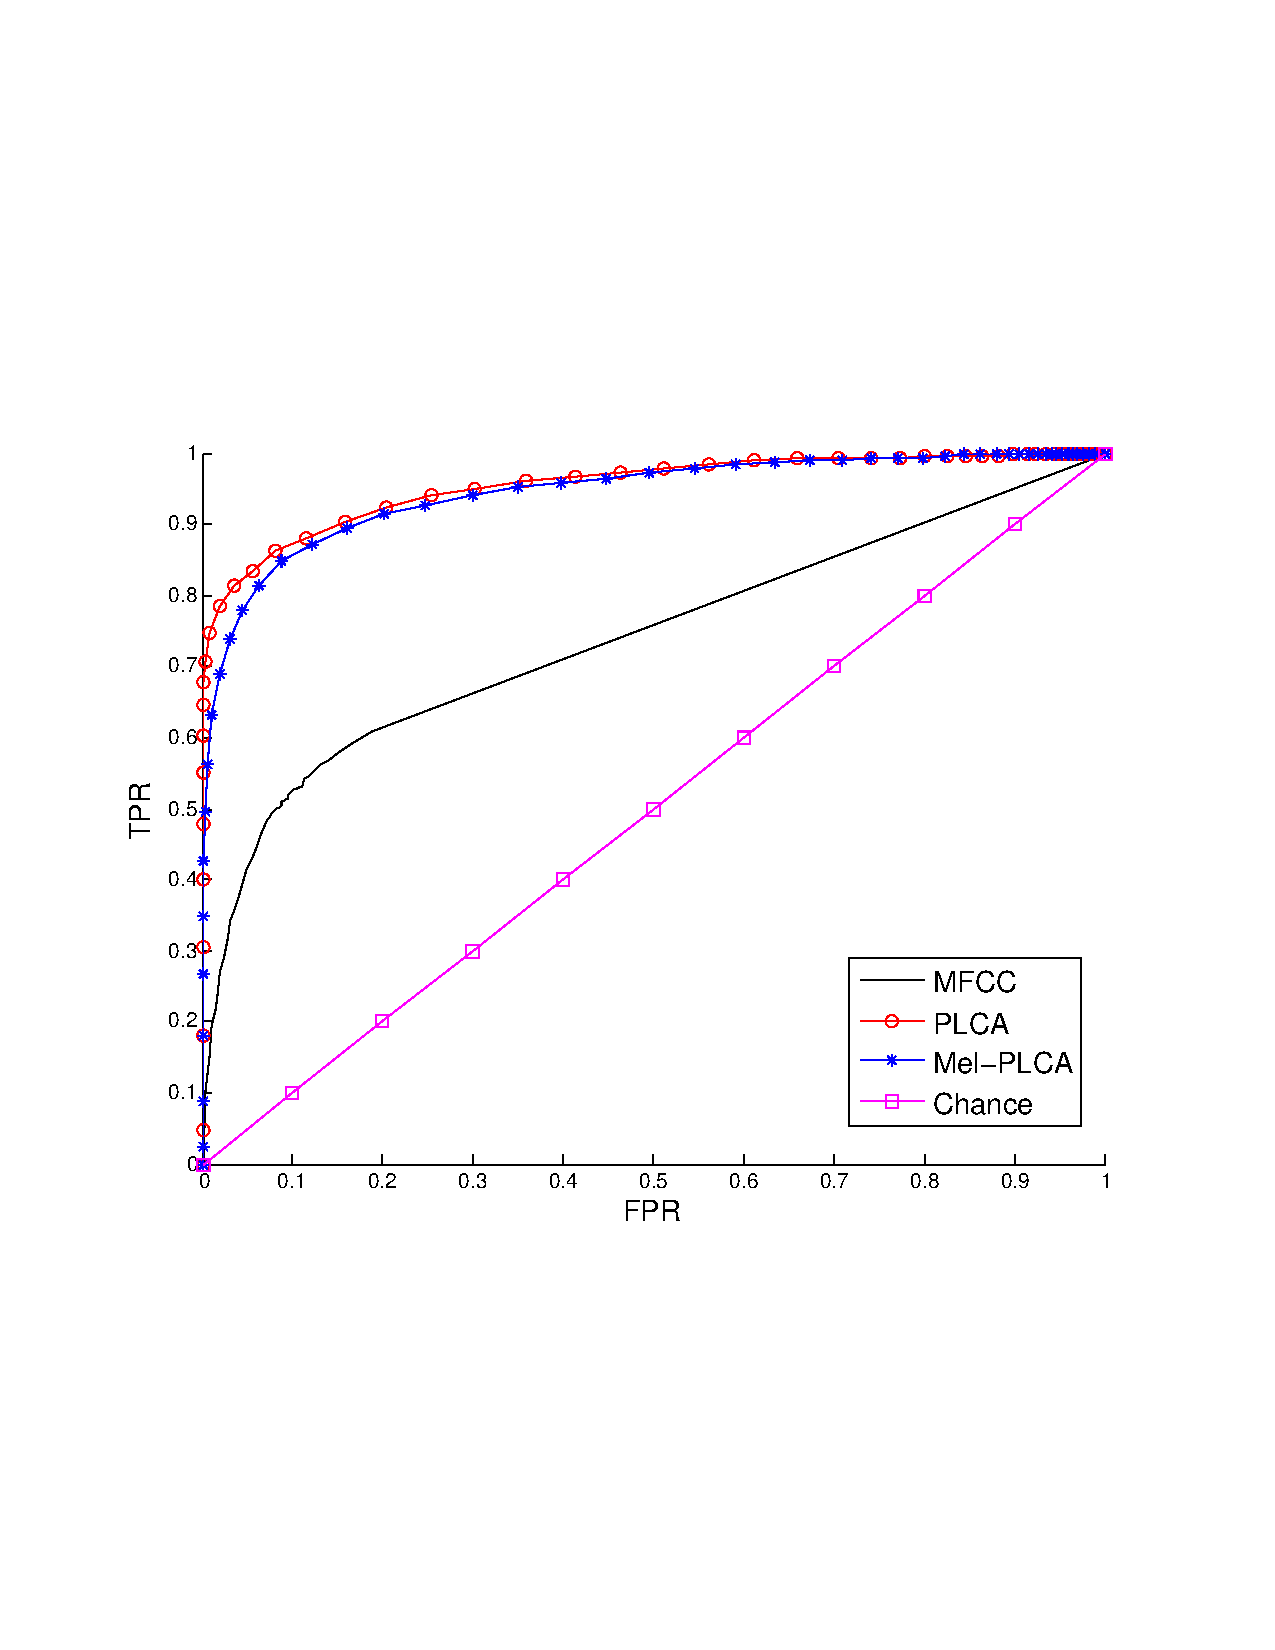
\includegraphics[width=0.99\textwidth]{images/mixture-roc-results.pdf}
		\caption{Experiment 3: Classification of acoustic mixtures.}
		\label{fig:mixture-roc-results}
	\end{subfigure}
	\caption{Results of Experiment 2 and 3 as depicted by the ROC curve.  The area under the curve summarizes greater model performance.  In both cases, the PLCA model outperforms the Mel-PLCA model which outperforms the MFCC model.}
\end{figure}

We tested the performance of both the MFCC and PLCA-based classifiers in the presence of noise by mixing one of 36 trained classes with an untrained class of sound (the 37th class), effectively masking the trained class with noise.  The average results of 1332 mixtures are depicted in Figure \ref{fig:unknown-mixture-roc-results} using ROC curves depicting each model's performance in classifying the correctly masked class.  We can see the MFCC model does well above chance, though both of the PLCA models do a much better job.  Interestingly, the Mel-PLCA model is very close to the performance of the full-spectrum based PLCA model, even though this model uses only 40 samples versus 8192 samples per frequency frame.

\subsection{Experiment 3: Classifying mixtures of acoustic events}


\begin{figure}
\begin{adjustwidth}{-6em}{-6em}
\centering
\begin{subfigure}[b]{0.55\textwidth}
\centering
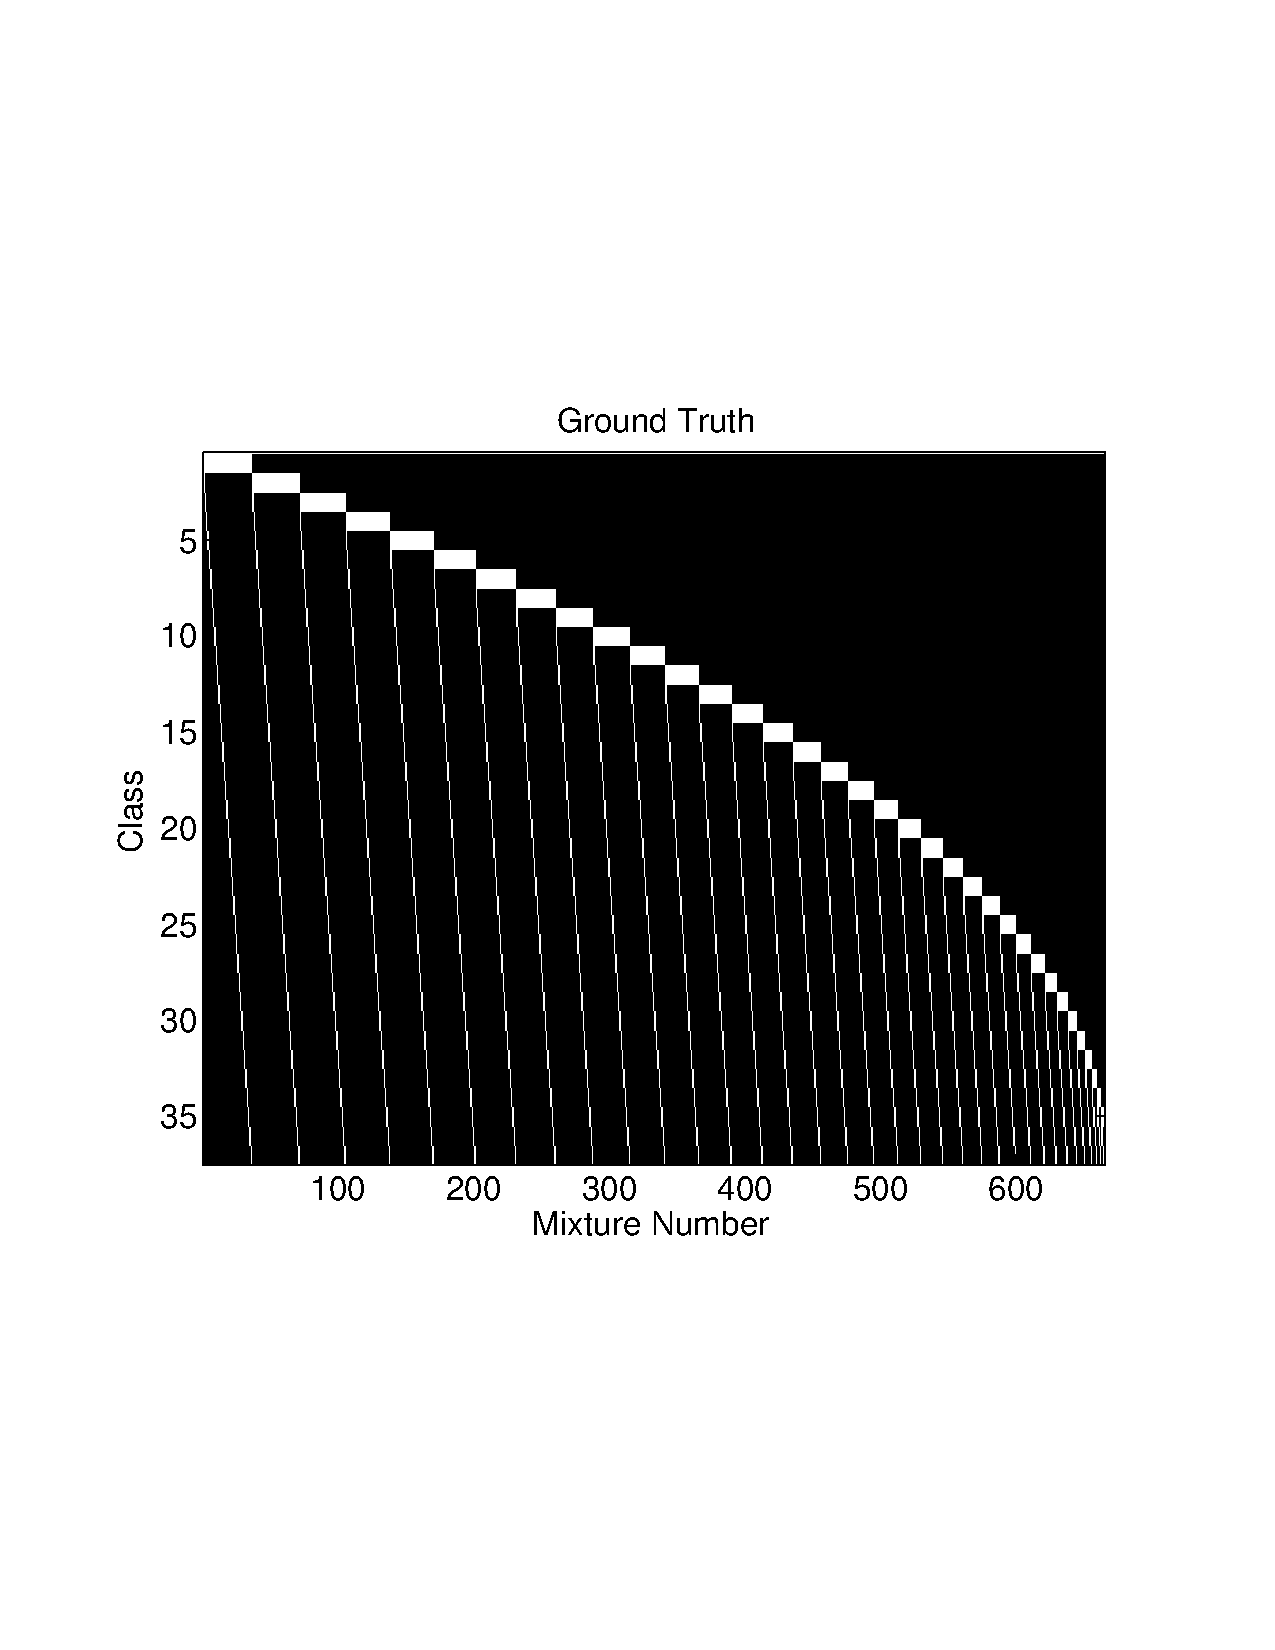
\includegraphics[width=0.99\textwidth]{images/mixture-groundtruth.pdf}
\caption{Ground truth labeling}
\end{subfigure}%
\begin{subfigure}[b]{0.55\textwidth}
\centering
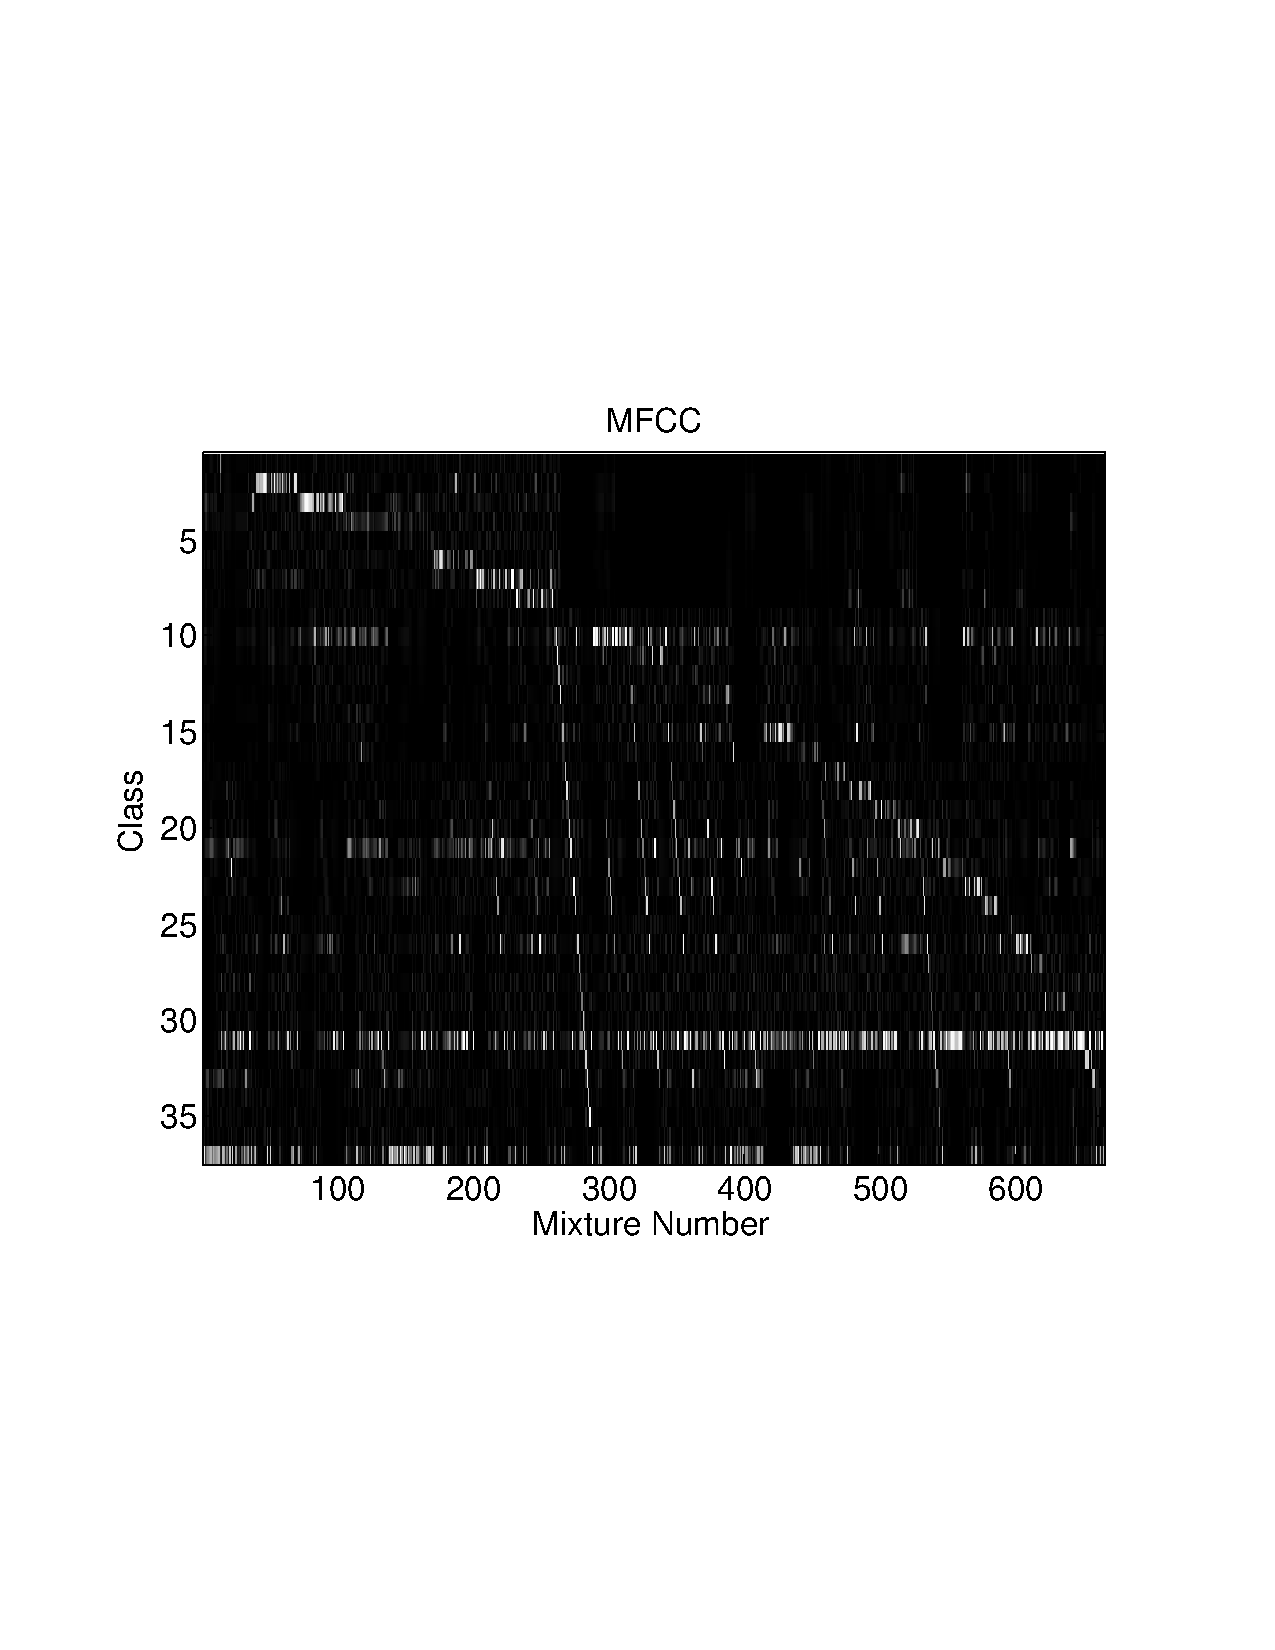
\includegraphics[width=0.99\textwidth]{images/mixture-mfcc.pdf}
\caption{Results for MFCC}
\end{subfigure}%

\begin{subfigure}[b]{0.55\textwidth}
\centering
\includegraphics[width=0.99\textwidth]{images/mixture-plca.pdf}
\caption{Results for PLCA}
\end{subfigure}%
\begin{subfigure}[b]{0.55\textwidth}
\centering
\includegraphics[width=0.99\textwidth]{images/mixture-melplca.pdf}
\caption{Results for Mel-PLCA}
\end{subfigure}%
\end{adjustwidth}
\caption{Experiment 3: Classification performance of acoustic mixtures depicting the ground truth classes for each of the 666 mixtures and the MFCC model, the PLCA model, and the Mel-PLCA model's classification likelihoods for each of the 666 mixtures. Images represent likelihood of a class in a given mixture, with white being 1.0, and black being 0.0.}
\label{fig:mixture-images}
\end{figure}

The last experiment measures the ability of our 3 models to classify both classes in an acoustic mixture of 2.  The results depicted in Figure \ref{fig:mixture-images} show the ground truth for the 37 possible classes across all 666 mixtures (${37 \choose 2} = 666$ classes) as an image.  This figure shows the likelihoods assigned to each of the 37 classes across all 666 mixtures for each of the 3 models.  From these figures, we can see the performance of the MFCC model struggles to classify most of the mixtures accurately, and often produces a false positive for classes 10 (conversation), 21 (laughing-man), and 31 (sword).  Thresholding columns of this image and storing the $TPR$ and $FPR$ as described in Section \ref{sec:ROC} produces 666 ROC curves.  The average of these curves are depicted in Figure \ref{fig:mixture-roc-results}, showing the performance of the MFCC model to be well above chance, though with the PLCA and Mel-PLCA models doing far better.  Interestingly again, we find the Mel-PLCA model is able to perform nearly as well as the PLCA model, performing within 0.01 of the PLCA model's AUC.  


\begin{table}
\centering
\caption{Area Under the Curve of ROC Analysis}
\begin{tabular}{|c|c|c|c|l|} \hline
Method&Experiment 1&Experiment 2&Experiment 3\\ \hline
MFCC&\textbf{1.0}&0.7388&0.7410\\ \hline
PLCA&\textbf{1.0}&\textbf{0.9303}&\textbf{0.9548}\\ \hline
Mel-PLCA&0.9989&0.9065&0.9443\\ \hline
\end{tabular}
\end{table}

% The methods presented can be extended to do generalizable acoustic event classification by training multiple classifiers representative of the variety of events that describe each class.  However there are three issues with any solution based purely on frequency information.  First, there is a dependence on microphone responses.  As microphone responses create a filter on the frequencies able to be represented, determining events on a headset quality microphone using classifiers trained on a studio quality microphone will be very difficult.  Second, different compression rates will also affect the representation of frequency bands creating artificial banded filters.  Lastly, how sounds may be recorded will also create ``filters'' of sound that can affect the representation of frequencies describing a sound.  For instance, in comparison to sounds heard in front of a listener, sounds heard behind a listener have a ``low-pass'' filter on the frequency responses.  

\section{Discussion}

We developed 3 computational models for the encoding and decoding of auditory scenes and tested their performance in the context of acoustic classification.  All 3 models performed with near perfect results when a single acoustic class appeared in isolation.  However, when the event was masked by an unknown acoustic class, effectively adding noise, the performance of the MFCC model dropped, though still performed well above chance.  The remaining models based on PLCA performed much better.  Our last experiment tested the performance of each model to classify multiple parts of an acoustic scene by mixing 2 classes together, effectively requiring segregation.  The MFCC model again performed well above chance with an AUC of ~0.74, but the models built with PLCA again performed with much stronger results, exhibiting > 0.9 AUC.

One possible reason for the poor performance of MFCCs during classification of mixtures is the signal model assumes a single excitation source (e.g. vocal tract or instrument).  In the presence of multiple sources, ambiguity is created, making it difficult to estimate which source contributes to each of the coefficients, especially since the sources are also combined non-linearly through the step of a log-transformation. 

Two disadvantages of using a full and direct spectrum model such as our ``PLCA model'' noted by \cite{Casey2001a} is their inconsistency and dimensionality.  We therefore tested a second model similar to the MPEG-7 spectral basis decomposition described in  \cite{Casey2001a}, ``Mel-PLCA'', which reduced the 16384 point Fourier spectrum to a 40 element vector.  However, unlike the MPEG-7 spectral basis decomposition, we made 2 significant changes: (1) we made use of the Mel-frequency scale rather than log-decibel scaling and normalization; and (2), as the article in question was written nearly 12 years ago, the only basis methods described were SVD/ICA/ and PCA based methods as PLCA had not yet been published.  Incorporating these changes, we found that the Mel-PLCA model performed within 0.03 of the full-spectrum PLCA model.  Using the critical bands defined by the Mel-frequency scale ensures the inconsistencies that may be apparent within similar acoustic classes are averaged out, and perceptually relevant frequency dimensions describing the class are retained while keeping dimensionality very low.  

\section{Future Work}

A number of viable extensions are possible.  First, as we only made use of highly textured atmospheric sounds, it remains to be seen whether the following method alone would suffice in modeling more impulsive sounds, e.g. drums, birds, or less atmospheric sounds.  In such cases, an entropic prior on the temporal weights of a PLCA decomposition would very likely greatly improve results \cite{Smaragdis2007}, ensuring the sparsity of temporal weights in the latent distribution $p(t|k)$, while capturing the bulk of the frequency distribution in the latent factor $p(f|k)$. 

Second, 2D patch-based and shift-invariant convolutive pLCA \cite{Smaragdis2007} has shown great promise in capturing the structure of music when applied to chromagram features and when using sparsity and shift-invariance in all features \cite{Weiss2011}.  Such a technique has the power not just for classifying the instruments that describe a musical passage, but as well the course of events that describe the musical scene, essentially identifying whole musical passages or riffs.  

Third, In real-time scenarios, it is often the case that a dictionary of classes is not readily available.  Recent work describing the online-learning of dictionary elements using PLCA has shown great promise in performing real-time speech de-noising \cite{Duan2012}, resulting in components separating noise and speech.  Such a distinction has wide applications in fields such as surveillance and tele-presence technologies.  

Lastly, in developing this work, it became apparent that no standard publicly and freely available libraries for evaluating acoustic scene classification algorithms exists.  Though the problem is well noted in music information retrieval \cite{Casey2008b,Rhodes2010}, and recently addressed with databases such as the million song dataset \cite{Bertin-Mahieux2011}, no standardized databases have been developed as freely available archives in the general sound-based multimedia communities.  As such, testing the scalability of our approach proved very difficult, as we could only obtain 37 classes and a total of 1332 mixtures even though databases such as YouTube and typical multimedia archives are on the order of many millions.  Future work must therefore be done to help understand the scalability and performance across different approaches using a standardized database.  

\section{Conclusion}

The framework in Chapter \ref{ch:conceptual-audio} gave us the notion of the unit of audio for use within a scene synthesis collage practice.  This was described by an analytical auditory event.  In this chapter, we developed this analysis procedure by encoding and decoding simple auditory scenes composed of a single auditory event, and extended these analyses to more complex auditory scenes composed of multiple events.  We found that MFCC and PLCA were both highly successful at building template matches (i.e. described in Chapter \ref{ch:conceptual-audio} by a processing negativity) simple acoustic scenes that did not need to be segregated.  When a scene required segregation before matching however, the PLCA model outperformed the MFCC one (i.e. described in Chapter \ref{ch:conceptual-audio} by a mismatch negativity).

The evaluations presented here do not consider the integration of a very large corpus.  In Chapter \ref{ch:synthesis-audio}, we explore scene synthesis of much larger audio corpora, The Daphne Oram Collection.  Consequently, we also explore methods for integrating a large number of representations, effectively allowing only representations that are more deviant than others to be learned.  Finally, in Chapter \ref{ch:memory-mosaic}, we also extend the model developed here to incorporate Event Detection in order to create the real-time system of Memory Mosaicing.

%assumptions in what is segregated... should have used people .. .but even subjective no good... rep...


%\section{Conclusion}

%The computational models developed here will be extended in the next Chapter to include event segregation allowing for a real-time system of encoding and decoding.  

%%%%%%%%%%%%%%%%%%%%%%%%%%%%%%%%%%%%%%%%%%%%%%%%%%%
%%%%%%%%%%%%%%%%%%%%%%%%%%%%%%%%%%%%%%%%%%%%%%%%%%%
%%%%%%%%%%%%%%%%%%%%%%%%%%%%%%%%%%%%%%%%%%%%%%%%%%%
%%%%%%%%%%%%%%%%%%%%%%%%%%%%%%%%%%%%%%%%%%%%%%%%%%%
%%%%%%%%%%%%%%%%%%%%%%%%%%%%%%%%%%%%%%%%%%%%%%%%%%%
%%%%%%%%%%%%%%%%%%%%%%%%%%%%%%%%%%%%%%%%%%%%%%%%%%%
%%%%%%%%%%%%%%%%%%%%%%%%%%%%%%%%%%%%%%%%%%%%%%%%%%%



%%%%%%%%%%%%%%%%%%%%%%%%%%%%%%%%%%%%%%%%%%%%%%%%%%%
%%%%%%%%%%%%%%%%%%%%%%%%%%%%%%%%%%%%%%%%%%%%%%%%%%%
%%%%%%%%%%%%%%%%%%%%%%%%%%%%%%%%%%%%%%%%%%%%%%%%%%%
%%%%%%%%%%%%%%%%%%%%%%%%%%%%%%%%%%%%%%%%%%%%%%%%%%%
%%%%%%%%%%%%%%%%%%%%%%%%%%%%%%%%%%%%%%%%%%%%%%%%%%%
%%%%%%%%%%%%%%%%%%%%%%%%%%%%%%%%%%%%%%%%%%%%%%%%%%%
%%%%%%%%%%%%%%%%%%%%%%%%%%%%%%%%%%%%%%%%%%%%%%%%%%%




\onehalfspacing
\chapter{Computational Auditory Scene Synthesis}
\label{ch:synthesis-audio}
\minitoc
\doublespacing

%\section{Abstract}

%Memory Mosaicing is a real-time sonic collage experience employing a perceptually-motivated model for representating and attending to sounds. This model relates the ongoing auditory world to previously learned ``sonic memories''.  Using a mobile platform, a user of the system wears earphones listening to an augmented sonic world which relates the incoming microphone stream to previously segmented sound clips, or sonic memories, creating a ongoing mosaic of sonic memories.  The system starts with an empty knowledge-base of sounds and continually stores only the segments of sounds which are determined salient and unclassified by a machine listening model.  The engine for synthesis is concatenative, matching the incoming segments to the learned ''sonic memories''.  The experience works in real-time on an iPhone 3 and above and has interactive parameters controlling the synthesis engine as well as the ability to learn from the user's own music library.  The experience of the iPhone app is multi-fold, creating a novel platform for investigating the role of memory in perception or as compositional or performance tool which grows its own expressive capabilities the more it hears.

\section{Introduction}

The juxtaposition of fragments of sound as an arts practice has roots at least as early as music concrete, a compositional technique assembling various natural found sounds in order to produce a collage of sound.  Digital Sampling came in the 1970's allowing sound segments to be triggered using an interface such as a keyboard or pad.  More recent techniques have focused on corpus-based concatenative synthesis, where a target sound is matched to a stored database of segments or sounds (for a comprehensive review, see \cite{Schwarz2006}).  In this thesis, we focus on a collage-based technique called scene synthesis which assembles units created through the computational modeling of psychologically motivated representations thought to support perception.  The aim in building these units and re-assembling them within a collage-based practice is to open a dialogue into the nature of representation within perception.  

We have so far derived a conceptual framework for building auditory representations based on evidence in electrophysiology in Chapter \ref{ch:conceptual-audio} and started to develop this framework computationally in Chapter \ref{ch:analysis-audio}.  In particular, we demonstrated that our computational model described by Mel-Frequency Cepstral Coefficients (MFCCs) perform very well at encoding auditory scenes in cases where the entire scene must be integrated.  Further we demonstrated that when segregation or understanding the multiple sources in a scene is required, models based on Principal Latent Component Analysis (PLCA) perform very well and are much better suited than MFCCs.  

We now turn towards one practical development using the previously built computational models.   The hope is to better understand the applicability of these models to real-world and interactive settings, and also better understand where there are any missing pieces to our computational model and conceptual framework for producing collage-based work.  This practical output, \textit{The Daphne Oram Browser}, compares our MFCC and PLCA models within an interactive scene synthesis using a large corpus of auditory material.  This scene synthesis is presented to a user of an audio archive in the form of a 3D virtual browser where they can select any segments of sound and hear them played back in real-time as an interactive sonic-collage.  This output attempts to discover how the representations motivated in Chapter \ref{ch:conceptual-audio} and computationally modeled with PLCA may help researchers understand any inherent content-based relationships within the content of a large audio corpus.  In other words, by using the representations built using our computational models, the relationships are not based on the content's filenames or metadata, but based on the way the content sounds.  A successful representation will ideally be able to define any inherent relationships within the archive based on purely sonic aspects.

%Finally, we describe \textit{Memory Mosaic} a real-time auditory scene synthesis in the form of an iOS application.  This output will require the development of the last missing component of our conceptual framework, event detection, which explicitly defines events within a real-time stream of audio.  As motivated in our conceptual framework in Chapter \ref{ch:conceptual-audio}, event detection describes our ability to unconsciously detect change within an auditory scene.  The auditory units demarcated by this process are then encoded to produce, over time, a large database of sonic ``memories''.  Within this real-time experience, the current unit of sound is also decoded, effectively matching the segment to the closest previously encoded stream to produce a real-time scene synthesis. 

\section{The Daphne Oram Collection}

The Daphne Oram Collection presents a unique case-study for the study of auditory representations.  It contains over 120 hours of 1/4'' tape dating from 1957 onwards and includes studio compositions, radio plays, sound effects, lectures, and interviews related to the British electronic musician, Daphne Oram (31 December 1925 - 5 January 2003) \cite{Young2008}.  Researchers working to understand the archive want to know more about her, her compositional techniques, and her radically innovative instrumental technique of ``Oramics'' for creating electronic sounds.  They have thus recently begun the process of digitizing the archive and at the time of this study had digitized 60 hours of the collection.  This process requires converting the analog tape reels to digital lossless formats allowing them to markup the digital files with metadata, or any additional textual descriptions of the audio file.  However, as this process has gone on, researchers have realized that the archive contains many duplicates and very little to no metadata.  In an effort to aid the researcher's understanding of the contents of their archive better, we employed our representations to build a 3D visualization of the archive where the axes of the visualization refer to relationships between similarly represented material.  

Using two of the methods developed in Chapter \ref{ch:analysis-audio}, we focus on visualizing the Daphne Oram archive using the encoded representations in order to project the archive as a 3-dimensional visualization.  These two methods are: (1) discovering latent distributions of frequencies using a recently developed source separation algorithm, probabilistic latent component analysis (PLCA) \cite{SmaragdisRajShashanka}; and (2), using a widely-adopted multi-dimensional feature for speech, music, and general acoustic classification, the Mel-Frequency Cepstral Coefficients (MFCCs).  We cluster the data from either descriptor using Multidimensional Scaling and develop a 3D visualization that allows researchers to project the archive onto multiple dimensions of the data.  Finally, we report user-feedback from researchers of the archive using the 3D visualization tool.  

Our main contribution is in describing the impact of visualizing segregated streams of a large audio archive through a case-driven exploration of the work of Daphne Oram.  We compare the feedback from archivists using a visualization of latent timbre-relationships versus one using a perceptually inspired multi-dimensional feature, MFCCs, and find that PLCA is more effective at producing a meaningful visualization.  

\section{Related Work in Visualizing Audio Archives}

A number of previous approaches for visualizing large audio corpora have focused on the application of music-based corpora.  Some approaches to content-based musical information retrieval solutions require a user to search by example or performance, aiding retrieval when a user is unaware of exactly what they are looking for.  However, visualization of such retrieval methods often amounts to viewing lists of the $k$-most similar results of an explicit query, and thus any exploratory analysis of the corpus as a whole requires further research into approaches for visualization.  For instance, SMILE \cite{Melucci2000} presents a MIDI-keyboard for the user to ``perform'' a query, and results are presented based on how similar the MIDI sequences are to the performance.  Similar approaches built for more generic signal-based audio break a corpus into frequency information and further into fingerprints such as MFCCs or psychacoustic descriptors.  audioDB \cite{Casey2008c,Rhodes2010} for instance allows a user to input shingles (fragments of audio), or segments of an audio track for discovering similarities in an archive.  Other solutions such as Query-by-humming allow a user to hum/sing a tune in order to discover similar results (e.g. \cite{Wang2006a,Cartwright}).  The previous methods may be suitable for applications where a user has an explicit example query.  However, in exploring an archive, it requires the user to have a priori knowledge of what the archive already contains.

Early work in exploratory content-based visualization systems can easily be traced to the 1990's where Starfields were commonly employed.  Starfields are interactive scatter-plots that allow for zooming, panning, and selection for greater detail, allowing one to view an archive through interaction.  The Informedia Digital Video Library System (1994-1998) \cite{Himmel1998,Christel1998} is one such system making use of the Starfield visualization approach, which accesses over a tera-byte of video and presents the user with an interactive scatterplot organized by the user's query.  Beginning with the audio signal, Informedia-I uses the Sphinx-II speech recognition system to discover annotations of audiovisual material.  Adding these to any existing text-annotations from captions, they create a term-document frequency matrix for each video segment, where segments are determined through the use of motion-based video-cut detection.  They are then able to discover latent relationships using PCA for reduction and visualization.  Other approaches such as IVEE \cite{Ahlberg1995} allowed for visualization options such as Tree Maps, Cone Trees, and even 3D scatterplots, though were not rooted in content-based information retrieval and instead relied on explicit relations of existing meta-data.  Though these early works were not directed for musically-based archives, their approaches towards visualization and interaction are very similar to ours, as we also look for latent relationships for reduction and visualization.

More recently, CataRT \cite{Schwarz2008} approaches Starfield style visualizations of large audio corpora by computing low-level psychoacoustic descriptors of grains segmented from a corpus for the purposes of composition, orchestration, and texture synthesis.  Visualizing the resulting mappings occurs in a 2D space where each axis is defined by a descriptor chosen by the user.  Such a visualization has the benefit of user awareness and control over the mappings that define a parametric spatial mapping.  Plumage \cite{Schwarz2008} extends the CataRT visualization into a 3D space creating a performance and composition environment where grains are colored, textured, and morphed in 3D space based on their psychoacoustic descriptions.  nepTUNE \cite{Knees2006} and \cite{Dominik2009} are two approaches to visualization which create a 3D terrain-style virtual space.  Songs are clustered using a self-organizing map of acoustic similarity in order to create virtual islands and terrain based on their clustering density.  The created virtual space thus encourages exploration and navigation of the visualized corpus.  \cite{Bartsch2001}'s approach employs the use of chroma-features for producing audio thumbnails of tracks, or segmented versions of an audio track encoding heavily repeated structures of harmonic relationships.  Though their approach is well-suited for popular music archives, they note that it is not suitable for music that does not obey a simple ``verse-refrain'' form.  Another approach uses mood words to describe a 3D interactive visualization, though relies on having access to socially tagged music in order to represent the music archive \cite{Stewart2008}. A more recent approach explored the use of MFCCs to describe an unknown corpus of audio and explore the audio using a 2D visualization created with a self-organizing map \cite{Heise2012}.  

The critical deviation of our approach to feature analysis from the previous approaches is by defining a 3D space using the corpora's own latent frequency distributions.  As we make no assumptions to the structure, perceptual relevance, or harmonic nature of the corpus, using probabilistic latent component analysis, we can discover the archive's own predominant distributions of frequencies and are able to use this reduced dimensionality dictionary as a representation of a high-dimensional space.  When projecting any 3-dimensions, the user is able to navigate the archive in a manner similar to CataRT \cite{Schwarz2008}. However, the axes are not user-defined psychoacoustic descriptions, but rather are projections of the archive onto ``timbres'' defined by latent frequency distributions (i.e. the encoded representations).  Our work similarly encourages exploration and navigation as in  \cite{Knees2006,Dominik2009,Heise2012}, though takes a information-centric point of view to analysis and retrieval.   We build a second visualization using a model which does not take into account the density of the data but instead uses a perceptual frequency transformation for building decorrelated features, MFCCs, similar to \cite{Heise2012} and report the user feedback for each visualization.

\section{Methods for Visualization}

Currently, the Daphne Oram Archive has over 215 tape reels or 60 hours digitized.  As the amount of available memory is a constraint on our approach, we are only able to investigate the first 10 minutes of the first 60 tape reels or 10 hours in total.  We describe each half second segment by their frequencies over time, described using the short-time Fourier transform, and describe each time-frequency matrix as a slice.  In total we have 1200 slices per tape and 72,000 slices for all 60 tape reels\footnote{We use all data for building the description of the corpus, though later use a reduced subset for visualization.}.  We aim to visualize this data using a clustering algorithm able to extract the timbre-relationships within the archive.  Specifically, we look at two methods for grouping the possible interesting frequencies describing the archive: (1) PLCA, a probabilistic method for discovering latent component relationships of a time-frequency matrix, and (2) MFCC, a widely-adopted approximation of the frequency spectrum inspired by the human auditory system's response properties.

\subsection{PLCA Model}
We use the basic model for PLCA as described in Section \ref{sec:plca} for encoding the entire archive.  However, one important extension is required, as with the basic PLCA model, the number of components describing a distribution must be known \textit{a priori}.  We therefore incorporate model selection, a commonly employed information theoretic approach to determining parameters of a model.  In the case of PLCA, the model parameters are described by $N$, the number of components or encoded representations to use.  We could use as many components as we have slices, producing 72,000 components.  However, this would likely over fit the database.  To appropriately determine the correct value for $N$, we use \textit{Bayesian Information Criterion} (BIC) model selection.  Using the log-likelihood of the optimized parameters, an additional parameter which penalizes model complexity is subtracted from the log-likelihood:
\begin{equationb}
\ln{p(X)} \simeq \ln{p(\mathcal{D}|\theta_{\mathtt{MAP}})} - \frac{1}{2}M\ln{N}
\end{equationb}
where $M$ is the number of parameters in $\theta$ and $N$ is the number of data points.  BIC ensures that we do not let the model overfit to a large value of $N$, while still producing a suitable log likelihood explanation of the observed data.

To begin the model selection, we iterate through every slice of audio.  Using model selection, we compare the results of using the current number of components and using an additional component.  If the results are better explained with an additional component, we add one to the value of $N$ and continue to the next slice. Iteratively running PLCA across all slices on increasing values of $N$ until finding the maximum BIC results in finding $N=45$ for 10 hours of audio.  

\subsection{MFCC Model}
For our second model, we use Mel-frequency Cepstral Coefficients (MFCCs), as described in Section \ref{sec:mfcc} which approximates a frequency spectrum by a set of de-correlated features.  

\subsection{Multi-dimensional Scaling}
After running each model, we are left with an $M \times N$ dimensional matrix, where $M$ refers to the number of time slices, and $N$ to the number of dimensions that describe each feature.  In the case of PLCA, after running model selection, we are left with $N=45$ dimensions describing the data.  With regards to MFCCs, we specifically choose $N=13$ cepstral coefficients.  

In order to visualize the high-dimensional space created by either model and cluster together similarly weighted features, we make use of Multi-Dimensional Scaling (MDS), a popular technique for multivariate and exploratory data analysis. MDS is a common technique for projecting data in high-dimensional spaces to 2 or 3 dimensional spaces for the purposes of visualization.  It aims to preserve the pairwise distances between data points, starting with the notion of distance, and working backwards in order to create the coordinate space.  The basic algorithm for calculating the unknown low-dimensional coordinate map $\mathbf{X}$ thus starts with a distance or proximity matrix, $\mathbf{P}$.  We aimed to use the full archive of 72,000 slices, however creating a matrix of float values this large requires $~20$ gigabytes of information which must be held in RAM.  Therefore, we reduce our database by taking every 5th slice, effectively looking at 0.5 second slices every 2.5 seconds rather than every 0.5 seconds.  However, the description of the data in the case of PLCA is still dependent on all 72,000 slices.
  
In order to calculate the low-dimensional coordinate matrix, we calculate the largest eigenvalues of the distance matrix after applying a double centering procedure.  The basic MDS algorithm is summarized as follows:
\begin{enumerate}
\item Compute a $M \times M$ proximity matrix $\mathbf{P}$ by calculating the Euclidean distances between each of the $M$ features
\item Compute the inner product matrix $\mathbf{B}$ by applying double-centring to the proximity matrix $\mathbf{P}$: 
\begin{equationb}
\mathbf{B} = -\frac{1}{2}\mathbf{J}\mathbf{P}^{(2)}\mathbf{J}
\end{equationb}
where $\mathbf{J} = \mathbf{I} - n^{-1}\mathbf{1}\mathbf{1^{\mathtt{T}}}$ and $n$ is the number of objects.
\item Compute the eigenvalue decomposition and retain the $n$ largest eigenvectors, $\mathbf{e}_1, ..., \mathbf{e}_n$ in order to compute the $n$-dimensional coordinate matrix $\mathbf{X}$:
\begin{equationb}
\mathbf{X} = \mathbf{E}_n\mathbf{\Lambda}_n^{\frac{1}{2}}
\end{equationb}
using the eigenvectors $\mathbf{E}$ and eigenvalues $\mathbf{\Lambda}$ of $\mathbf{B}$ 
\end{enumerate}

One may also notice the algorithm is equivalent to a doubly-centered version of PCA in the case where the distances are Euclidean.  As both the PLCA and MFCC model's feature dimensions are de-correlated, we would expect to find the number of eigenvalues approach the same dimensionality as either model.  Thus, the PLCA model is clustered in 45 dimensions, and the MFCC model in 13.


\section{Graphical User Interface of the Browser}

\begin{figure*}
  \centering
  \begin{adjustwidth}{-12em}{-12em}
  \centering
  \includegraphics[width=1.25\textwidth]{images/gui.pdf}
  \end{adjustwidth}
  \caption{Screenshot depicting the GUI of the browser (best viewed in color).  Here a user is currently inputing text in order to annotate one of the sound segments.  We can see sliders to the left allowing the user to zoom in/out, change the dimensions of the visualization, and control which elements are drawn on screen.  With all of the options being drawn, we see the waveform of the currently highlighted sound (depicted with a white cube under the mouse cursor) is drawn on the bottom.  The meta-data describing the file name is just below the waveform.  To the right, the decibel-scale spectrum is also drawn.  All elements are drawn in real-time and are interactively manipulated in 3D space.}
  \label{fig:gui}
\end{figure*}

The interface is shown in Figure \ref{fig:gui} and is built in C/C++ using the creative-coding toolkit openFrameworks\footnote{http://www.openframeworks.cc}.  The user is presented with a 3D space (see Figure \ref{fig:gui}) where each slice of sound from the archive is represented as a cube projected in 3D space.  The coordinates of the cube are determined by which dimensions of the MDS coordinate matrix are selected.  To begin, the first three dimensions are displayed.  Users can then select any dimension to be displayed on the 3-axes.  As a result, the visualization can also be constrained to a 2D visualization by simply choosing the same dimension for 2 axes.  A colormap is used to help depict distance from the OpenGL origin (using a ``jet'' colormap, i.e.: blue-yellow-red), though the user can turn this off.  Figures \ref{fig:oram-browser-plca} and \ref{fig:oram-browser-mfcc} depict the visualizations  of the first three dimensions produced using MDS inside the browser.  

While inside the browser, pressing space-bar allows one to annotate the currently selected slice.  The annotated text appears in 3D next to the slice's cube.  The slice's audio is also visualized as a waveform and its instantaneous Fourier transform.  As we used the first ten minutes of every tape-reel, the waveform for any given slice is presented as a looped region within a 10 minute audio file.  However, the user can change the loop regions to hear any other portion of the original audio file while selecting a slice, thus allowing the user to listen to the audio before and after the slice.

The user can also move the camera around the OpenGL origin by dragging the left mouse button in the 3D space.   Highlighting any of the cubes with the mouse allows the user to inspect the clip in greater detail.  Taking a cue from the 2D analog CataRT, any of the cubes can be ``scrubbed'' for playback by simply moving the mouse over any of the cubes, not requiring any further interaction to listen to the sound sample.  Zooming in and out of the 3D space can be done via the mouse scroll wheel or graphical slider.  Double-clicking on any of the cubes re-centers the origin to the selected cube, allowing camera interaction to occur with respect to the cube.  Cubes can be spaced closer or farther from each other using another graphical slider.  This allows more tightly clustered portions of a visualization to be explored in greater detail.  

%Describe how you derived the PLCA model
%Describe how you derive the MFCC model
%Descirbe the MDS stuff
%Describe how you created the visualisation
%Describe the user studies and how the interface evolved
%State that we worked with the users to make the interface more usable.


\section{User Feedback}\label{results}

Three researchers of the Oram Archive were invited to navigate the browser and spent 1 hour in total using both the PLCA and MFCC visualizations.  They were unaware of how either model was created, were unfamiliar with signal processing and machine learning, and were only told that we are investigating a way to navigate the Oram Archive.  Each user was given 5-10 minutes of explanation of the features of the browser and were then left to explore the browser by themselves.  Each user proceeded to explore the archive by using the mouse to listen to the different slices located in 3D space.  In addition, each user managed to find particularities of the archive that seemingly would have been very difficult without the browser.  For instance, finding a significant portion of one tape reel that was labeled as ``POP TRY-OUTS'' in another reel labeled as ``COPY DONKEY HELL ABC \& ITV. BIRDS \& PERC'' by exploring slices located near each other in the 3D space.  Also, one found components relating to Daphne Oram's piece, ``Birds of Parallax'' during lectures series that were only labeled by their location, indicating she demonstrated these components during her talk.

When asked to compare the two visualizations and remark on their usability as a navigation tool of the Daphne Oram Archive, the three researchers reported on the form of the MFCC model in comparison to the PLCA one, saying (1), ``it has a less useful shape in general'', (2) ``it has less detail'', and (3) ``this dense mass represents total variety...and I don't quite understand how it is mapped.''  In response, we asked what if anything made the PLCA model more useful for navigation in comparison to the MFCC model.  User 1 reported: ``it has a more definite and understandable space. For example, prongs that have specific information in them such as silence.'' and User 3 reported: ``Oh that's really successful, it seems to be matching pitch and you start to see how she was using pitch'' and ``I had a clear sense of how it was mapped''. 

Each user also gave many helpful possible extensions to the current functionality of the browser, including the ability to save camera states, only view a particular reel's slices, and auto-zoom and rotation around a particular point.  User 1 found the 3D nature of the visualization required more practice saying they ``might get used to it'' while User 3 commented on navigating around a single slice saying ``I understand it as a structure, but I'm working out where in 3D space [the slice] is.  You have to move around in 3D before working it out.''   User 3 also expressed the scope of the browser for new users to see and appreciate Daphne Oram's work, remarking, ``Goes to show just how much variety there are in the samples, and this has made that variety accessible.''  

User 2 additionally remarked on the potential of incorporating other mediums of Daphne's work saying it would be great to ``include other mediums than audio, combining with video/letters/images.''  Both User 2 and User 3 commented on the tool's applicability to performance and composition, saying he/she was ``fascinated as a compositional tool.  Navigating different dimensions, it's a beautiful instrument'' and ``it is nice to categorize sounds as it is what we do in sampling''.  

\begin{figure}
  \centering
  \begin{subfigure}[b]{0.45\textwidth}
  \centering
  \includegraphics[width=\textwidth]{images/plca-1.png}
  \end{subfigure}     
  \hspace{0.5pt}
  \begin{subfigure}[b]{0.45\textwidth}
  \centering
  \includegraphics[width=\textwidth]{images/mfcc-1.png}
  \end{subfigure}     
  
  \begin{subfigure}[b]{0.45\textwidth}
  \centering
  \includegraphics[width=\textwidth]{images/plca-2.png}
  \end{subfigure}     
  \hspace{0.5pt}
  \begin{subfigure}[b]{0.45\textwidth}
  \centering
  \includegraphics[width=\textwidth]{images/mfcc-2.png}
  \end{subfigure}     
  
  \begin{subfigure}[b]{0.45\textwidth}
  \centering
  \includegraphics[width=\textwidth]{images/plca-3.png}
  \caption{PLCA model}
  \label{fig:oram-browser-plca}
  \end{subfigure}     
  \hspace{0.5pt}
  \begin{subfigure}[b]{0.45\textwidth}
  \centering
  \includegraphics[width=\textwidth]{images/mfcc-3.png}
  \caption{MFCC model}
  \label{fig:oram-browser-mfcc}
  \end{subfigure}     
  
\caption{Screenshot of the first 3 dimensions of the PLCA and MFCC models visualized in the browser.  We show three different views here.}
\label{fig:oram-browser}
\end{figure}




%Describe the results of the user studies and how this resulted in changes to the interface.
%Describe that the MFCC model made a far worse visualisation according to the users. DONT discuss why yet.
%Describe how the users responded to those changes
%Detail a few areas where new information was gathered about the recordings.
%Describe how some of our metadata was verified and more clearly understood - we found components relating to Daphne Oram's piece "Birds of Parallax".

\section{Discussion and Future Work}\label{discussion}

Each researcher had prior knowledge of many aspects of the Archive and Daphne Oram's composition techniques, and were also familiar with many of the recordings.  Their interests in the archive stemmed from her methods in composition to the actual electronics of the Oramics Machine.  When given the chance to navigate the archive in a 3D space arranged by acoustic similarity, each user was incredibly pleased by the possibilities and results of just one hour's navigating, and also preferred the PLCA model to the MFCC one generally for 3 reasons: (1) the visual form and structure of the PLCA model was easier to navigate, as knowing where one was in 3D space is easier to notice, (2), navigating within the ''glob-like'' mass of the MFCC representation in 3D required users to go inside the sphere, making interaction very difficult, and (3), the mapping and clustering in the PLCA model appeared more intuitive, with users reporting they understood how it was mapped and the similarity of sounds along a projection seemed to cluster sounds better.  

Regarding (1) and (2), the form of the PLCA model (see Figure \ref{fig:oram-browser-plca}) is a result of the probabilistic nature of the component weights needing to sum to 1.  In 3D space, this space is defined by a 3-simplex or tetrahedron.  In comparison, MFCCs may have energy explained in all bands as there is no normalization procedure.  Plotting the first three dimensions of the MFCC model thus produces similar distributions of energy in all dimensions, creating what users called both a ``glob like'' and ``blob like'' sphere (see Figure \ref{fig:oram-browser-mfcc}).    Navigating inside and around a sphere presents unique challenges for a 3D browser, namely, it is difficult to select elements within the sphere and understanding the orientation of the sphere is difficult as there are no identifying features.  Thus, exploring visualizations in 3D seems to require landmarks for useful navigation.  In regards to point (3), this may be due to the greater classification and recognition performance of PLCA over MFCCs as shown in Chapter \ref{ch:analysis-audio}.  

Further work should focus on issues with navigating in 3D space, as some users reported on the 3D nature as requiring practice to navigate.  One solution may be to create more intuitive control through the use of other input and display devices such as touch-screens.  Similar latent-analysis techniques may also be applied for additional meta-data from the archive as is done in audiovisual and text corpora, e.g. \cite{Himmel1998,Christel1998}, to create more informed visualizations.  In this case, the input of text annotations as well can create a user-guided visualization, where feedback from the user reshapes the 3D visualization.  

Lastly, incorporating event detection, as motivated in our conceptual framework in Chapter \ref{ch:conceptual-audio}, would provide automatic segment lengths, rather than fixed half-second segments as used here.  Such a framework would be capable of describing latent factors based on temporal windows of uniform spectrums rather than arbitrary segments.  This arbitrary segmentation may include multiple events or incorrectly cut off an existing event, thus reducing the power for PLCA to describe its latent factors when building the dictionary.  

\section{Conclusion}

This chapter has discussed the first practical output towards employing auditory scene synthesis in the form of The Daphne Oram Browser.  It has taken the conceptual framework presented in Chapter \ref{ch:conceptual-audio} and as modeled computationally in Chapter \ref{ch:analysis-audio} in order to develop an analysis of a large corpus of auditory material.  This analysis displays The Oram Archive as a 3D interactive visualization allowing for real-time scene synthesis via a simple mouse cursor.  We will later see how incorporating a computational model of event detection for analyzing a large audio corpus can be used for creating real-time auditory scene syntheses in Chapter \ref{ch:memory-mosaic} and for offline processing of YouTube videos in Chapter \ref{ch:audiovisual}.

%%%%%%%%%%%%%%%%%%%%%%%%%%%%%%%%%%%%%%%%%%%%%%%%%%%
%%%%%%%%%%%%%%%%%%%%%%%%%%%%%%%%%%%%%%%%%%%%%%%%%%%
%%%%%%%%%%%%%%%%%%%%%%%%%%%%%%%%%%%%%%%%%%%%%%%%%%%
%%%%%%%%%%%%%%%%%%%%%%%%%%%%%%%%%%%%%%%%%%%%%%%%%%%
%%%%%%%%%%%%%%%%%%%%%%%%%%%%%%%%%%%%%%%%%%%%%%%%%%%
%%%%%%%%%%%%%%%%%%%%%%%%%%%%%%%%%%%%%%%%%%%%%%%%%%%
%%%%%%%%%%%%%%%%%%%%%%%%%%%%%%%%%%%%%%%%%%%%%%%%%%%



%%%%%%%%%%%%%%%%%%%%%%%%%%%%%%%%%%%%%%%%%%%%%%%%%%%
%%%%%%%%%%%%%%%%%%%%%%%%%%%%%%%%%%%%%%%%%%%%%%%%%%%
%%%%%%%%%%%%%%%%%%%%%%%%%%%%%%%%%%%%%%%%%%%%%%%%%%%
%%%%%%%%%%%%%%%%%%%%%%%%%%%%%%%%%%%%%%%%%%%%%%%%%%%
%%%%%%%%%%%%%%%%%%%%%%%%%%%%%%%%%%%%%%%%%%%%%%%%%%%
%%%%%%%%%%%%%%%%%%%%%%%%%%%%%%%%%%%%%%%%%%%%%%%%%%%
%%%%%%%%%%%%%%%%%%%%%%%%%%%%%%%%%%%%%%%%%%%%%%%%%%%



\onehalfspacing
\chapter{Conceptual Framework for Building Unconscious Visual Representations}
\label{ch:conceptual-visual}
\minitoc
\doublespacing

\section{Introduction}

This thesis has so far seen how scene synthesis may occur within audition.  Certainly, the issue of perception tackled by our brains must functionally find similar outcomes in vision as it does in audition (e.g. discover representable aspects of the world and be able to function with them).  Still, these domains require individual treatment as we employ fundamentally different behaviors when using either modality.  One obvious reasoning for this is that movements of the eye allow us to spatially orient within the visual world, whereas within audition, no similar action exists.  However, this should not be taken to mean that these domains are independently processed in the brain.  Clearly, many multisensory and crossmodal effects have been demonstrated (e.g. the auditory override of visual perception as demonstrated in the double flash illusion \cite{Shams2002} and the visual override of auditory perception as demonstrated in the McGurk effect \cite{MCGURK1976}).   However, only so much can be explored within this thesis, and we therefore work towards a modal solution in the hopes that the interactions within the two modalities could be explored in the future.

Similar to aims in developing the framework for audition in Chapter \ref{ch:conceptual-audio}, conceptualizing an overarching framework for visual perception is beyond the scope of this thesis.  Even if it were within the scope, we have only really begun to understand the some 1 million retinal ganglion cells \cite{Curcio1990} or the estimated 140 million neurons in early visual cortex \cite{Leuba1994}, let alone how the remaining 5 higher cortical layers or inferior temporal cortex and fusiform areas may possibly effect early layers of processing.  There is a great amount of work to be done before a comprehensive model can be achieved.  Therefore, this chapter limits its discussion to seminal research within the physiology and behavioral psychology of visual perception.  From these select few readings, we aim to develop a plausible conceptual architecture that will inform the implementation of the computational model developed in Chapter \ref{ch:analysis-visual} and used in practice for producing visual scene syntheses in Chapter \ref{ch:synthesis-visual}.

\section{Background Literature on Visual Perception}

\subsection{Early Theory}

In a seminal thesis on visual perception in 1915, Edgar Rubin describes a fundamental form of experience consisting of a figure standing on a ground \cite{Rubin1915}.  The figure describes the focal or fundamental experience of a scene, whereas the ground describes the ambient or marginal portions of a scene.  Expanding this point further in the 1920's, the Gestalt psychologists developed a comprehensive perceptual theory employing figure-ground as a fundamental type of perception where the notion of a Gestalt, or totality, is described by a set of rules describing the formation of a figure and ground.  These rules included:

\begin{itemizeb}
\item \textbf{Similarity}: Entities sharing physical properties in terms of size, color, or other visual features, are grouped to form the same figure
\item \textbf{Proximity/Contiguity}: The smaller the distance between two entities, the more likely we are to group them together
\item \textbf{Symmetry}: Objects in symmetrical alignment can be perceived as the same figure even if they do not have close proximity to one another
\item \textbf{Good continuation}: Grouping of a pattern of visual features beyond what we can see
\item \textbf{Common Fate}: Grouping of the same temporal movements
\item \textbf{Closure}: Filling in missing pieces to complete a figure
\end{itemizeb}

Effectively, the ``Gestalt'' describes the fundamental experience of perception.  As a result, any subdivision or interrogation of a part of the Gestalt would alter experience into yet another figure and ground relationship \cite{Koffka1935, Kohler1947}.  Though these rules provide a good logical understanding of how figures may be described, understanding how our brain represents or discovers such relationships is still a very open question.  

\subsection{Visual Physiology}

From these early studies describing logical rules for grouping, visual perception research has continued in trying to understand how the brain could possibly encode the formation and understanding of such figures.  The physiology and behavior of the eye alone has given researchers an enormous understanding of the processes supporting perception.  Starting with the physical wavelengths of light entering our eyes, we rapidly shift our gaze an average of 3-5 times a second, completely disrupting the continuity of light entering our eyes.  Visual acuity limitations mean that our eyes require rapid ballistic movements of the eye taking all of 30 ms (a \textit{saccade}) to project the light from the particular point of a visual scene we are interested in onto a 2-degree area of the retina with the highest spatial resolution (the \textit{fovea}), finally stabilizing our eyes to the region of interest (a \textit{fixation}), a process lasting on average 330 ms.  During this time, it is thought that the encoding of details at the point of fixation into memory occurs as well as planning of the next eye-movement \cite{Henderson2003,Findlay2003}.  

Going away from the fovea (the \textit{parafovea}), resolution for spatial detail drops logarithmically, while resolution for motion detail increases.  This relationship is explained (1) by the refractivity of light afforded by the lens of the eye itself, (2), the distribution or density of cells in the fovea is more tightly clustered than in the parafovea, and (3), the response properties of the individual cells (also defined as ``receptive fields'' \cite{Sherrington1906}) of photo-receptive cells including retinal ganglion and their connections along the optic tract to lateral geniculate nucleus (LGN) cells \cite{Curcio1990}.  Other connections from the ganglion cells in the eye extend along the optic tract to the superior colliculus where it is thought that encoding of the control of eye-movements in retinotopic coordinates occurs \cite{Klier2001}.  

%\hl{Stuff about color here... }

Connections from the ganglion cells travel along the optic tract eventually extending all the way to the back of the brain to the occipital lobe where the visual cortex resides.  Seminal research demonstrating physiological evidence of the receptive fields and the discovery of 'simple' receptive field cells in the early visual cortex (the first of six cortical layers, denoted as V1) of cats \cite{Hubel1962} and monkeys \cite{Hubel1968} has helped to better understand the early processing  occurring in the brain (for which David Hubel and Torston Wiesel later won the Nobel Prize in 1982).  The authors explain that: 
\begin{quotationb}
These fields were termed 'simple' because like retinal and geniculate fields (1) they were subdivided into distinct excitatory and inhibitory regions; (2) there was summation within the separate excitatory and inhibitory parts; (3) there was antagonism between excitatory and inhibitory regions; and (4) it was possible to predict responses to stationary or moving spots of various shapes from a map of the excitatory and inhibitory areas.
\flushright{\cite{Hubel1962}}
\end{quotationb}  
Hubel and Wiesel's work demonstrated the ability for such cells to effectively respond with higher magnitudes whenever presented with contrast changes of certain sizes and orientations, depending on their contrast specificity, and to more complex gratings that respond to the change of a stimulus in all directions (center-surround).  Despite these early findings, to date, there is still no generally agreed upon classification of cortical receptive fields within the scientific community.  However, one that has been most widely used is the response to sinusoidal gratings at different scales and orientations.  These are typically modeled by Gabor filters (2D Gaussian multiplied by an oriented sinusoid, where the positive regions of the sinusoid refer to the excitatory and the negative to the inhibitory regions), however even this widely used approximation has raised some criticism, as it bypasses modulations occurring between the retina and V1 (i.e. within the Lateral Geniculate Nucleus) \cite{Azzopardi2012}.  Effectively this literature has demonstrated that cells in V1 can respond in a selective manner to a variety of different features in the visual scene including line orientation, direction and speed of movement, luminance and luminance contrast, color and color contrast, retinal disparity, and spatial frequency \cite{Rao1999a}.  

Cortical analysis of motion stimuli also shows that the majority of V1 cells have selective response to motion in different orientations before sending their output to the medial temporal cortex \cite{Palmer1999}. It thus does not seem surprising to find that evidence based on search efficiency has shown that our visual system is able to notice moving objects even if we are not looking for them.  Such phenomena associated with parts of a scene that eventually attract our attention and gaze are often given the label ``pop out''.   It is further thought that given evidence of the electrophysiology of monkeys, the encoding of an actual map prioritizing locations likely to ``pop-out'', also denoted as a \textit{saliency} map, is likely to exist in the lateral intraparietal cortex (LIP) and the frontal eye fields (FEF) \cite{Gottlieb1998,Kusunoki2000,Moore2003,Thompson2005}.  Saliency representations in LIP are thought to encode either abrupt onsets, stimulus motion, or task-dependent, behaviorally-relevant stimuli \cite{Gottlieb1998,Kusunoki2000}.  Other studies have demonstrated that the electrical stimulation of sties within retinotopic maps in FEF were likely to evoke saccades to the retinotopic site of the target and could even suppress responses coming from visual cortex \cite{Moore2003}.  A later study also demonstrated that responses in FEF were independent of any explicit saccade command signals \cite{Thompson2005}, further suggesting that the FEF is likely to encode attentional biases and modulate ongoing visual processing.  

As evidenced by the physiology of the eye, LGN, and early visual cortex, our periphery has been engineered for high motion resolution rather than high spatial resolution.  Therefore, we cannot encode with high spatial detail an entire visual scene at once, as a camera with a small aperture may be able to do.  Instead, we actively view a scene in order to perceive its details.  This entails the use of saccades and head-movements in order to perceive with greater detail the parts of a scene required for our ongoing tasks.  Many researchers in visual cognition have therefore focused their research in understanding eye-movement behavior, investigating why, where, and under which circumstances we move our eyes.  Loosely, this research can be defined by the field of visual attention.

\subsection{Visual Attention}

The earliest studies \cite{Buswell1935,Yarbus1967} describe two main influences of a viewer's attention to a visual scene: (1) influences dependent on mental states which focus attention towards contextually and cognitively relevant aspects of the world (\textit{endogenous}), and (2) influences dependent on involuntary capture of attention from the external environment (\textit{exogenous}).  As exogenous factors are involuntary, one would expect to find the behavior influenced by these factors to be highly consistent across viewers.  In contrast, as endogenous influences are dependent on cognitive factors resulting from emotion, memory, language, task, and previous experiences, the relationship of a scene and one's endogenous influences on the scene are much less consistent across viewers.  

\subsubsection{Exogenous Influences on Attention}
\label{sec:exogenous-attention}
In seminal work investigating the speed of visual perception using Gestalt-like primitives, Sziklai demonstrated the human visual system exhibits an attentional bottleneck of 40-bits per second on selected information, suggesting our visual systems require a simplified representation from the many megabytes per second of information coming from exogenous visual information \cite{Sziklai1956,Merrill1968}.  Much research investigating exogenous influences on static visual scenes therefore describe a simplified representation of attentional control in what they originally called \textit{bottom-up} models \cite{Koch1985,Itti1998,Wolfe1989,Itti2001}.  These models attempt to explain how we possibly allocate processing or plan a future saccade to certain regions, features, or objects in a visual scene while also dealing with the many overlapping, occluding, or other difficulties in continually recognizing objects in natural scenes.  

Early bottom-up models are built upon theories of feature-integration \cite{Treisman1980} and are modeled based on the response properties of simple receptive field cells.  There are also denoted in the literature as ``saliency'' models of attention, though this was before the discovery of attentional maps within LIP and FEF.   To discover the attentional biases for portions of a scene, bottom-up models start with a camera image and filter it using a series of filter banks tuned to multiple frequency orientations and scales to produce a set of conspicuity maps.  Effectively, this process discovers oriented edges and color contrasts within an image at different orientations and scales.  Saliency is then defined by a weighted linear summation (\textit{integration}) of the resulting conspicuity maps. 

It is further suggested that the final integration within bottom-up models are modulated by what Itti et. al calls ''top-down'' influences \cite{Itti1998,Itti2001}.  Within their model, they implement an inhibition-of-return measure which is based on evidence of longer reaction times measured with the return to a previously cued or fixated location \cite{Posner1984,Posner1985,Klein2000}, though cite that other influences from the current ongoing task \cite{Yarbus1967,Smith2011a} and the context of a scene in order to reduce processing load \cite{Henderson2003,Torralba2006} are likely to effect this map.  

If we take these bottom-up models as a literal translation to early cortical filters, and the resulting integrations as those denoted in FEF or LIP, then the level at which top-down influences may actually affect processing is still an open research question.  For instance, it may be that top-down effects do reach V1 or more likely at least V2, thus effecting the formation of filter bank maps (e.g. \cite{Rauss2011}).  Further, though these modulations are often described as top-down influences, such a term should not be confused with endogenous influences, as much research has shown that memory, context, and other endogenous factors affect early visual processing \cite{Tatler2011} which would correlate with initial feature stages thought to be unaffected in a bottom-up model.  

Gist-based models (presented later) separating ``conceptual'' and ``perceptual'' influences may similarly be looked at in terms of ``bottom-up'' and ``top-down'' influences, or even ``exogenous'' and ``endogenous'', respectively.  Another common distinction is the notion of 'covert' attention, or influences dependent on internal visual attention systems or the ability to attend to a peripheral location, and 'overt' attention, essentially eye-movements.   However, even this distinction has been criticized as they may not be independent given the complicated and interconnected nature of attentional mechanisms \cite{Findlay2003a}.  As a result, there appear to be a variety of confounding terms introduced by this literature which were intended to help the understanding of processes in the brain.  However, they all vary slightly in their use and meaning across literature, which should be no surprise given the complicated nature of the brain.  We therefore attempt to restrict our use for the purposes of this thesis and refer to only endogenous and exogenous processes (as other researchers now also do, e.g. \cite{Soltani2010}), as these terms seem to offer the most useful definition separating influences originating from the brain and from the sensorial world, respectively.  Other distinctions, e.g. bottom-up/top-down, are therefore not used given their possibly ambiguous meanings. 

Early saliency models focused their investigation of attentional biases towards static scenes.  Rosenholtz however investigated how attention would shift in the context of motion-based stimuli.  In her 1999 study, she created a measure of saliency based on the extent to which the motion of a scene differed from the general pattern of the scene \cite{Rosenholtz1999}. She showed that a simple model measuring motion outliers can detect motion pop out phenomena reliably.  Itti et al. has since incorporated measures of motion into the most recent versions of the iLab Neuromorphic Vision C++ Toolkit for their saliency computations \cite{Itti2005b}.  

Despite significant efforts, some researchers have claimed that the attentional biases within early saliency models would not translate to the real-world \cite{Henderson2003,Tatler2009a,Tatler2011}.  One reason is suggested by the fact that the stimuli used to motivate the early saliency models were composed of randomly placed letters such as t's and l's.  Certainly the responses within V1 may describe a priority map within such simple scenes, as one misplaced letter would create a strong center-surround response in V1.  In fact, it has even led some researchers to suggest that V1, V2, or V4 may be the site of the saliency map, despite only ever testing their hypothesis on simple psychophysical stimuli \cite{Li2002,Soltani2010a,Zhang2012a}.  Further, endogenous influences to saliency as modeled in early saliency maps were primarily based on the notion of inhibition of return in static picture arrays \cite{Posner1984,Posner1985,Itti1998,Itti2001}.  However recent research suggests this inhibiting effect does not occur in dynamic scenes \cite{Wang2010} or given the presence of sudden onsets \cite{Smith2009a}.  Essentially, the real-world is not composed of simple statistical features and is in fact much more complex and certainly dynamic, if not even for our own motions within it.  As a result, there has been a trend to move away from understanding behavior in simple psychophysical scenes and to use eye-tracking within real-world complex scenes to better understand behavior \cite{Henderson2003,Tatler2009a,Tatler2011}.

\begin{figure}[!ht]
\centering
\includegraphics[width=\textwidth]{images/diem-lab-space.png}
\caption{Left to right: (a) Original image of frame 1975 of video 24 (\textit{Video Republic}: \url{http://www.demos.co.uk/publications/videorepublic}); (b) L* image depicting luminance (Lum); (c) a* image depicting red/green opponent colors (RG); (d) b* image depicting blue/yellow opponent colors (BY)}
\label{fig:diem-lab-space}
\end{figure}

\begin{figure}[!ht]
\centering
\begin{subfigure}[t]{\textwidth}
\centering
\includegraphics[width=\textwidth]{images/diem-gabor-construction.png}
\caption*{The process for creating a log-Gabor kernel for 0 degrees (left to right): (a) the radial map computed from multiplying a sinusoid with a Gaussian kernel; (b) the orientation of the kernel set for 0 degrees; (c) the result of multiplying the radial (a) and orientation (b) maps; (d) the even symmetric component of the log-Gabor filter taken from the real part of the inverse Fourier transform of the kernel; (e) the corresponding odd symmetric component taken from the imaginary component of the kernel.}
\end{subfigure}
\vspace*{5pt}
\begin{subfigure}[t]{\textwidth}
\centering
\includegraphics[width=\textwidth]{images/diem-gabor-edges.png}
\caption*{Left to right: Gabor oriented maps for (a) 0 degrees, (b) 45 degrees, (c) 90 degrees, and (d) 135 degrees for the luminance image in Figure \ref{fig:diem-lab-space}}
\end{subfigure}
\caption{We investigated a feature resembling the response properties of cells found in early visual cortex, a Gabor filter.  These effectively model edges at different orientations and scales.  In our original manuscript, we tested these on a set of 4 orientations and 2 scales.  The top figure demonstrates the process of creating the filter, while the bottom demonstrates the output of 4 orientations.}
\label{fig:diem-gabor-construction}
\end{figure}

\begin{figure}[!ht]
\centering
\includegraphics[width=\textwidth]{images/diem-motion.png}
\caption{Left to right: (a) High pass flicker (Flicker); (b) Low pass flicker (Flicker-N); (c) Horizontal optical flow (U-Flow); (d) Vertical optical flow (V-Flow) for the frame in Figure \ref{fig:diem-lab-space}}
\label{fig:diem-motion}
\end{figure}

\begin{figure}[!ht]
\centering
\includegraphics[width=\textwidth]{images/diem-2x2-baseline-fixations.png}
\caption{Example of actual (cross) and baseline (circle) subject fixations.  Baseline fixations are created by randomly sampling the distribution of all fixations in a given movie for each frame.}
\label{fig:diem-baseline-fixations}
\end{figure}

\begin{figure}[!ht]
\centering
\includegraphics[width=\textwidth]{images/diem-auc.png}
\caption{Area Under ROC Curves (AUC) as a function of weighted cluster covariance (bins=75).  The results here demonstrate the ability for motion features (top-most lines) to discriminate actual and baseline fixations better than any other feature.  Further, as participants are more tightly clustered (going left on the x-axis), the discriminability of most visual features goes up.}
\label{fig:diem-auc}
\end{figure}


Certainly, behavioral evidence demonstrating exogenous attentional biases within dynamic scenes is greatly evidenced by eye-movement recordings \cite{Itti2005,Carmi2006,Mital2011}.  In a previous study, we investigated the contribution of a set of different visual features to gaze location during free-viewing of dynamic scenes \cite{Mital2011}.  Of these features, we included a set of edge oriented filtered images created using Gabor filters, similar to those found in visual saliency models (see Figure \ref{fig:diem-gabor-construction} for an example of their construction).  We also attempted to measure the correlation of gaze behavior with a set of dynamic features such as the frame-to-frame difference in luminance and also a measure of optical flow \cite{Horn1981} (see Figure \ref{fig:diem-motion} for an example).  Optical flow simply attempts to measure a frame-to-frame registration, discovering how luminance values in a scene shifts thus trying to recover not just the magnitude of motion but the oriented vectors of movements in the recorded image over time.  It also controls for consistency in a scene by ensuring smoothness across a scene similar to processes of lateral inhibition, while still affording sharp discontinuities likely to occur at object borders through a data penalty term (often l1-normalization).  In order to control for our experiment, we compared fixated locations to a randomly sampled baseline created from the distribution of all fixations in each film.  In other words, we wanted to see if actual fixations could be distinguished from randomly sampled ones using a particular visual feature (see Figure \ref{fig:diem-baseline-fixations} for an example of the baseline fixations).  Our results (shown in Figure \ref{fig:diem-auc}) indicated that fixated locations could be discriminated from control locations (randomly sampled from the distribution of all fixations) by optical flow as the strongest predictor, beating all static features including oriented and differently scale edges and corners, mid-level features thought to be encoded in V2 such as corners, and even simple dynamic features encoded in many saliency models such as flicker (simple frame-to-frame luminance differences).  

%\hl{put in diem investigation roc curves?} 

%\hl{Clustering of gaze during dynamic scene viewing -> motivate flicker as an attentional map, prior to understanding temporal incoherences, sets basis for proto-object representation later... discuss attentional synchrony paradigm... }
  	
\subsubsection{Endogenous Influences on Attention}
\label{sec:endogenous-influences}

Despite the overwhelming influences of certain visual features such as motion to attract our attention, simple task manipulations can easily override these biases.  One of the first demonstrations of an endogenous influence on eye-movement behavior investigated eye-movements during static scene viewing \cite{Yarbus1967}, Yarbus tracked the eye-movements of participants viewing a painting entitled, ``An Unexpected Visitor.''  His study showed that when participants viewed the painting and were given a task such as to determine the ages of the people in the painting, they looked more at the faces of each person.  When asked to determine what they were wearing, their eye-movements strayed away from faces, and looked more towards the clothing of people.  Yarbus further describes 7 different tasks and shows how the eye-movements of each participant reflects the information required for processing the task at hand.  Since then, numerous studies have expanded on their results, suggesting endogenous influence that can override exogenous influences \cite{Tatler2009}.

In a similar study though with dynamic scenes instead of a static painting, we investigated task-based effects on viewers' eye-movements looking at unedited videos of natural scenes from a camera mounted on a tripod \cite{Smith2011a,Smith2013}.  Participants were natives to the city of Edinburgh and viewed a variety of indoor and outdoor scenes from the city.  Our study revealed that during free-viewing, i.e. not given any task other than to look at the video, participants looked at mostly moving objects such as people moving across the frame or cars, as described by a computational model of flicker or optical flow.  However, when given the task to identify the location of the presented scene, participants had to concentrate their gaze towards the elements of a scene depicting landmarks such as buildings, signs, and trees and showed a remarkable ability to distract away from moving objects.  As a result, flicker and optical flow were far less likely to predict gaze locations.  Though, after viewers pressed a button indicating recognition of the location, their viewing behavior reverted to resembling the free-viewing task, fixating on moving objects such as people and cars again.  Our study also re-asserted the findings of Yarbus, though for a dynamic time-course.  Further, it also provided evidence of default viewing conditions during the time-course of viewing, as participants were able to ``return'' to the free-viewing task after having finished the task of recognizing the location of the scene.  

The manipulation of the task in our previous study demonstrates the ability for us to build up a representation of a scene by focusing on the details of the scene.  In the free-viewing case, this entails looking at moving elements.  However, it is likely not the moving elements in of themselves that are necessary for scene understanding, but rather the social figures that are moving.  In this case, the understanding of the scene is likely depicted by activities occurring in the scenes, and these happen to require movements.  In the case that our task is not focused on social understanding of the scene, as in the spot the location task, we must draw our attention away from the social elements.  In this case, the background elements and their arrangement are more likely to have details about the scene's location, as they may provide landmarks to discovering the location.  

%\hl{Discovering social or contextual biases towards a scene is not an easy one, considering the great amount of possible tasks.  Some work depicting street scenes has shown that a simple horizontal filter can increase predictability of gaze (Torrabla.. .)... more stuff like this?  }

%\hl{Discuss use of attentional synchrony paradigm in smith paper and in Melissa's paper too...}
%\hl{attention is indexed by proto-objects, reference roi analysis, ante's study jov 2010}
%\hl{building up representation .. fd/sa}
%\hl{binding attention to maintain.}

\subsection{Gist}
\label{sec:gist}

%\hl{Introduce RSVP. then introduce gist more before saying what its findings entail...}
Given that we are constantly moving our eyes and radically altering the light coming into our retina, how much can we encode in the short amount of time we spend when fixating?  Researchers wanting to better understand the same question created a paradigm called rapid serial visual processing (RSVP), where a fixation cross would appear followed by an image that would be presented for a short amount of time.  In their original study, participants were tested for details of a scene presented for only 100 ms and performed very well \cite{Potter1969}.  When they were asked to do the same thing given a series of images that were presented rapidly and with the same duration, their performance went to chance levels \cite{Potter1976}.  However, when given either a pictorial or verbal a cue to the image to remember details of (\textit{priming}), their performance went to significantly better than chance performances with the pictorial cue performing at about 80\% and the verbal one at 60\% \cite{Potter1969,Potter1976}.  It should be noted that despite the 100 ms presentation time, it would take participants a longer amount of time before they were able to report the content of the scene.  This is likely due to the limits of conscious processing (e.g. as demonstrated by the P3 ERP component).

From these studies, it was understood that we can rapidly encode information about a pictorial scene with a presentation lasting only 45-135 ms (\textit{Gist}) \cite{Potter1969,Biederman1974,Potter1976,Schyns1994,Henderson1999}.  Extensions within this body of research have suggested that we likely encode the general shape and structure of a scene in order to infer its context.   Further, a number of theories have suggested that this shape is defined by either volumetric forms (\textit{geons}) \cite{Biederman1987}, spatial arrangement of blobs defined by contrasts in luminance or color \cite{Schyns1994,Oliva1997} or by using a scene's spatial frequency content \cite{Oliva2001,Oliva2005}.  Spatial frequency content can be described by oriented band-pass filters: at a low spatial frequency, this content resembles broad edges and the layout and orientations of a scene's largest similarly textured regions, whereas at a high-spatial frequency, the response of the sharpest edges and their directions are encoded.  

Endogenous influences on gist processing seems to influence the spectral scale at which gist is selected \cite{Schyns1994,Oliva1997}.  Schyns and Oliva describe an experiment where a low-spatial frequency (\textit{LSF}) and a high spatial frequency (\textit{HSF}) image are created for two separate pairs of images.  Creating two new images by combining the LSF of one image and the HSF of the other, and vice-versa, they investigate the scale space of gist recognition with and without a verbal cue to indicate what type of scene will follow.  Without priming, subjects are able to recognize the scene described by the LSF content of an image given 45 ms of presentation time, and the HSF one within 135 ms.  Subjects are also unaware of the content in the other scale space (i.e. shown an image with LSF and HSF content for 45 ms, the participants are unaware of there being separate HSF content).  However, being primed with either the LSF or HSF content of the scene, subjects report perceiving the given cue instead.  

While gist is thought to be pre-attentive, i.e. before the timescale of acts of selective attention, such research suggests either that (1) the scale at which the early representation of gist operates at is affected by task-demands (i.e. only one scale of gist is encoded for pre-attentively), or (2), attention and further encoding into memory is dependent on endogenous influences on scale selection, (i.e. gist may be encoded at multiple scales, but only the scale selected by attentional machinery is encoded into memory).  Though not all scales are necessary for determining a scene's content when given prior cues (\textit{priming}), the neurobiology of early visual cortex gives scope for encoding of multiple visual scales.  It thus seems possible to assume (2) is a more likely model for the interaction of gist and attentional machinery.

%\hl{Talk about features diagnostic to a scene's description, and how they accelerate or impair recognition of a scene, e.g. color in natural environments (Oliva, 2005)}
%Oliva further argues for two types of gist, \textit{conceptual} and \textit{perceptual}.  Conceptual gist refers to semantic information inferred from viewing a scene or from shortly after a scene disappears. Perceptual gist is thought to be motivated by the given task at hand in order to provide the structure or form of a scene and uses pre-attentive low-level information such as color, orientation, depth, and motion (Oliva, 2005).  \hl{Need to explain these much more as they go back into proto-objects and should be related to endo/exo as well etc...}
	
Gist has been understood in terms of the classic rapid serial visual paradigm (RSVP), or within a screen based presentation where stimulus presentations are preceded by empty or noisy screens.  However, the real-world is not preceded by such screens, and rather the notion of gist across saccades in a situated and embodied world becomes an important one to make.  How does a dynamic real-world model of gist help us to maintain a coherent perspective of the world, and further guide our attention?  Research demonstrating our failure to notice dramatic changes within static and dynamic scenes may help us to decipher this question better.

\subsection{Change and Inattentional Blindness}
\label{sec:change-blindness}

Specifically, research demonstrating the failure to report large changes in the visual world (\textit{change blindness}) as well as the failure to report unexpected visible changes due to task requiring attention elsewhere (\textit{inattentional blindness}) \cite{Simons1999,Rensink2000,Rensink2001,Hollingworth2001a} have shown that our visual systems are unaware of changes in visual world outside of the point of fixation.  Simons and Chabris demonstrated \textit{Inattentional Blindness} by composing a video of two basketball teams dressed in white and black passing a ball to each other \cite{Simons1999}.  Participants were asked to count the number of passes that the white team makes.  During the course of the video, a person wearing a gorilla suit walks across the frame of the camera.  However it was unnoticed by 75\% of participants.  The selective attention mechanisms therefore seemed to not be able to encode the gross contextual violation of a gorilla within a basketball scene.  This seems to reveal some indication to the nature of representation outside of selective attention.  Namely, the semantic details of the entities outside of fixation are either (1) not encoded, or (2) encoded, but not able to be compared to any other semantic entities (as this would trigger some contextual violations, thus capturing attention). 

Another fascinating ``failure'' of the human visual system to detect large changes in the visual world is demonstrated by the phenomena of \textit{Change Blindness}.  As demonstrated in a real-world psychology experiment \cite{Simons1998}, participants arrived at a kiosk to fill in a consent form and handed the completed form to a man behind the counter.  The man ducked behind the counter as to pretend to file the paper, while a different man came up from behind the counter, again unnoticed by a majority of the participants.  In a similar demonstration, an RSVP paradigm displayed two different images separated by a transient of white-noise.  The white-noise effectively removed the capability of discovering the change between the two images.  That is, under a normal viewing circumstance, a gross change in a visual scene would likely capture attention due to the onsets of motion and changes in visual features of luminance and color.  However, removing these transients by placing a scene of white noise effectively removes the ability to detect transients of the previous scene.  Moreover, the memory representations retained from the scene pre-white-noise are such that post-white-noise, they are not challenged in any way (since they do not capture attention).  

In both change and inattentional blindness, the failure to detect changes outside of the point of fixation suggests that any peripheral representation of a scene would likely not encode details of object specific features such as color, motion, or orientation gratings.  Rather, our visual machinery integrates the detailed aspects of objects across eye-movements, retaining that information as a perceived representation of the visual world.  The broad spatial scale afforded by the lens of the eye and the higher motion resolution afforded by the spacing of cones in the periphery give further indication to the lack of highly detailed feature encoding in the periphery.  Though, to what form, and to what detail a periphery representation may encode is still an open question.  

%\subsection{Electrophysiology}\label{sec:electrophysiology}
%Visual Mismatch Negativity... reviews in Czigler 2007, 2010...
%\cite{Stefanics2011}
%Border-ownership in V2 modeled by lateral interactions, producing self-organizing structures resembling shapes.
%Violation of sequential rules elicited for a deviant color (Czigler 2002), orientation (Kimura 2010), movement (Pazo-Alvarez 2004), spatial frequency (Heslenfeld 2003), contrast (Stagg 2004), sequential conditional relationships (Stefanics, 2011), and even facial expressions (Zhao and Li, 2006)

\subsection{Visual Object Representation}

Despite the numerous occlusions, lighting changes, and possible angles at which we view an object, we continue to be able to recognize objects in all their possible slight variances.  We can even extract object representations from clouds, turkish coffee, and even linen cloths (e.g. Shroud of Turn \footnote{\url{en.wikipedia.org/wiki/Shroud_of_Turin}}).  The incredible feat here is not the grouping strategies for determining boundaries of an object, as suggested by the Gestalts, but rather the binding of these groups into semantic labels.  

Rensink takes evidence in change and inattentional blindness in developing a theory of coherence, proposing that object representation depends on focal attention.  He suggests that once attention is focused, a ``coherence field'' is established, linking the details at the point of fixation to a semantic object representation.  For objects outside of the point of fixation, Rensink proposes we encode volatile units of \textit{proto-objects} \cite{Rensink2000,Rensink2001}.  Proto-objects are argued to be amorphous and blob-like in nature, representational-less and concept-less lasting only a few hundred milliseconds.   It is further argued that attention operates on groupings of proto-objects rather than at the earlier feature levels making it the highest level of early vision, and the earliest operands of selective attention.  Rensink also hypothesizes that proto-objects may explain non-attentive processes capable of recognizing the abstract meaning of a scene and the spatial layout of the scene \cite{Rensink2002}.  In relation to perceptual influences, implicit behavioral measures suggest that grouping processes can also occur for task-irrelevant visual stimuli, i.e., for stimuli that has not been attended to by a fixation, further supporting theories of proto-object formation \cite{Lamy2006}.

\textit{Object files}, described by Kahneman and Triesman \cite{Kahneman1984}, suggests that visual objects are hierarchically described, with the higher levels denoting the semantic description of the visual object (e.g. a group of dancers), mid levels describing any possible parts making up the entity (e.g. individual dancer or the hand of the dancer), and the lowest levels describing the spatiotemporal constraints of the object itself.  Their theory suggests that attention describes the level that object files are accessed, and that they are kept open for a limited time as attention is withdrawn, effectively creating a limit to the number of object files that are kept open.  Coherence theory certainly resembles object files, though with one important distinction that once attention binds proto-objects into the coherence field, the field collapses as soon as attention is removed from it, leaving only the volatile proto-objects to collapse shortly after.  Thus, in Rensink's model, only one stable semantic representations seems to be active (in the coherence field), whereas in Object Files, there can be many open at any given time.  

Though these theories work towards an understanding of how the various processes of perception (e.g. attention, gist, representation), may interact, they do not yet paint a complete picture for describing a truly computationally implementable model.   This is because the descriptions of ``spatiotemporal'' constraints in object-files or the ``groupings'' of proto-objects are open to interpretation.  However, some understanding may be gained when considering Marr's seminal work in describing shape invariances \cite{Marr1978,Marr1982}.  Marr considered that perception must be 3-dimensional, and the goal of perception is therefore to reconstruct the images coming into the retina as a 3-dimensional scene.  He describes a transition from lines, to contours, to surfaces, and finally to volumes.  At the end of this process, Marr suggests that the representations held in the brain are defined by \textit{view-specific} ``sketches'' of this volumetric reconstruction.  Therefore, to recognize an object, we would have to have already encoded a set of ``sketches'' that were similar to the current view of that object.  

Biederman's Recognition-By-Components (RBC) offers another framework towards understanding representations, suggesting that the recognition of an object should be \textit{view-invariant} so long as one can encode an object's geometric-ions (\textit{geons}) \cite{Biederman1987}.  In Biederman's case, the representation of an object entails the encoding of a set of shapes in 3-dimensions, such that their relative groupings are also encoded (e.g. a sphere and a cylinder in some relationship describe a baseball bat).   In contrast to Marr's approach, one would only have to have seen one or a few views of an object, encoded their geons, and then any novel view of it would be decoded so long as the same geons could be detected.  

The distinctions between Marr and RBC-based approaches to object representation have continued to present day, labeling one camp as view-based, and the other as object-based.  It is likely that the human visual system is capable of discovering objects in either case, though discovering this is beyond the scope of this thesis.  What can be gained from this discussion, however, is the importance of shape to early object representation in either case.  Further, such theories suggest that a simpler primitive unit is necessary for ongoing scene perception and that it is not necessary to refer to the highly detailed representations of the scene until the task demands it (i.e. through fixating on a part of a visual scene).  

%\hl{Shape in cortex...}

%\hl{Object in cortex...}

%\hl{Neural Populations of Object Classes in Inferior Temporal Cortex... }

%\hl{Never discussed Dorsal/Ventral stream... is it necessary?}


\section{Conceptual Framework}

Taking this literature forward, we are now in a position to motivate a conceptual framework for a computational model of visual scene synthesis.  In particular, this literature has demonstrated the importance of an active viewing of a scene.  Though, in practice, accessing eye-movement information about a scene is not possible without an eye-tracker.  Thus, if we want to build a visual scene syntheses modeled by perceptual processes, we must develop a model of attention describing where we are likely to attend to.  This will allow us to describe any realistic visual scene in terms of higher spatial acuity at a point likely to be fixated.  In other words, we will encode details of a scene that are likely to be attended, where finer resolution details are encoded in parts of a scene more likely to fixated, and coarser details are encoded outside of these parts.  Following Rensink's Coherence Theory, we assume a representation for encoding and decoding described by volatile units of proto-objects within the scene.  His theory does not specify what these units may be described by, but other research proposed by Biederman and Marr have suggested the importance of shape to the encoding of proto-object-like structures.  As a result, these units should likely be described by representations encoding properties of their shape, color, and luminance.  The summarization of this model is below:

\begin{enumerateb}
\item \textbf{Exogenous Attention Model} Defines where one is likely to look in a dynamic visual scene.  Following our previous studies, \cite{Mital2011,Smith2013}, in free-viewing cases, this can be described by temporal irregularities within the visual scene (e.g. points of high contrasting flicker or optical flow).  This point will then define the computationally modeled ``fixation'';
\item \textbf{Visual Acuity} Physiologically, we have higher spatial acuity at the point of fixation than outside.  This means we should only encode coarser details outside of a fixation rather than try to encode an entire scene's high spatial resolution;
\item \textbf{Proto-Objects} Finally, the description of the scene can be defined by a collection of volatile units.  These should be described by color and shape-based representations taking into account the coarser resolutions outside of fixation due to visual acuity. 
\end{enumerateb}

%\hl{How this is a proxy for a very simple estimation of change, but we are very much capable of encoding higher order regularities... An example of how this is not true, a case where motion patters are learned, but some static pattern appears as being very unregular... No sense of semantic or contextual relevance, but this could be added by discovering scene layout... prioritize gaze to horizon... people... text... faces...}

%\hl{The entropy of the motion correlates to entropy of gaze locations... use this value to drive the acuity map then... }

%\hl{Spatial grouping of color, motion, and luminance cues.  Builds a shape representation.}

\section{Discussion}

Behavioral evidence from change blindness studies has indicated an essential gap in our encoding of a scene, namely the precise details of a scene are only encoded at the point of fixation.  This is likely due to the computational complexity required for encoding an entire scene's high-spatial resolution information.  More importantly, it is physiologically impossible given the visual acuity limitations of the retina.  Therefore, though we experience a rich, detailed visual world, we do not use such rich details in building a stable representation \cite{Simons1997}.  Rensink argues that object representation requires focal attention.  

In considering an architecture of visual perception, what is the cause of producing focal attention?  The literature presented here suggests that there is either an endogenous explanation or exogenous one.  In developing a computational model, it is feasible to build an implementation of the prioritization of exogenous attention across a visual scene, as our previous research has shown that motion is highly correlated with gaze capture and such a model is easy to implement.  However, in building an endogenous one, numerous factors would have to be considered for which many open research questions still exist: e.g. the influence of task.  We therefore leave this as an open limitation to our framework, and keep it in mind when discussing our final outputs, though hope it could be later extended to produce more interesting variations.  % For example, I may focus on a cup, but not build the representation of the fingerprints on the cups as I was not intending to look at this particular scale.  In this case, the endogenous influence of perceiving the object representation of fingerprints on the cup was necessary for building such a representation, even though focal attention will have brought my eyes to the cup.  It may be that my task of drinking from the cup saw the cup as what it afforded: a drink.  In a free-viewing task, or a task where no explicit instruction is given, it may be more likely that an exogenous influence such as the mis-representation of the cup will provoke more detailed representations and cause additional focal attention to the cup.  Thus, it may be the case that focal attention is necessary for explaining an object, however, it seems it is not sufficient and the cause of focal attention should still be considered.  

When considering evidence for gist in relation to Rensink's theory of coherence, it seems viable to consider proto-objects as the same representation that gist may use \cite{Rensink2002}.  Though Schyns and Oliva argue for using oriented banded filters, it is not unlikely that collections of blob-like entities which necessarily also respond to the scale of the proto-object could provide a cue for spatial layout.  However, when considering evidence in rapid determination of the meaning of scenes, Schyns and Oliva demonstrated that early processing of a scene could be re-organized based on prior experiences \cite{Schyns1994,Oliva1997}.  Thus, it is not clear from their research alone whether the pre-conceptual representation itself can be changed, or if only the attentional machinery acting on a set of possible representations has changed.  The latter effect would entail a sort of conceptual prior on a scene, suggesting the organization of a scene's early representation remains untouched.

Pylyshyn theorizes that the understanding of a concept is not all that is required for visual experience: 
\begin{quotationb}
''Vision suited for the control of action will have to provide something more than a system that constructs a conceptual representation from visual stimuli; it will also need to provide a special kind of direct (preconceptual, unmediated) connection between elements of a visual representation and certain elements in the world. Like natural language demonstratives (such as 'this' or 'that') this direct connection allows entities to be referred to without being categorized or conceptualized. \cite{Pylyshyn2001}''
\end{quotationb}  
The preconceptual connections Pylyshyn describes are easily described by the pre-attentive proto-objects Rensink also describes \cite{Rensink2000,Rensink2001}.  What is interesting in Pylyshyn's theory is the notion that this pre-conceptual representation does not need to be categorized or conceptualized in order to be referred to.  In other words, the categorization which Pylyshyn theorizes of is part of the attentional machinery which refers to proto-objects, rather than an explicit property of the proto-object themselves.  According to Pylyshyn's theory, proto-objects of a visual scene are then described by one particular fate, and attentional mechanisms can only select from the set of possible proto-objects, rather than influence their definition. 

Proto-objects act as an indexical reference to a conceptual referent.  How proto-objects are defined is based on the features that best give coherence to the scene.  They are also scaled with increasing eccentricity, presumably at least because of the shape of the eye would decrease spatial resolution, but as well due to the nature of attention acting at the point of fixation.  Functionally, visual material outside of the region is of less importance to the task at hand.  Thus, the biological nature of the shape of the eye could also be understood in terms of evolving to act in the world.  Proto-objects may also possibly find re-definition from the act of attention.  As proto-objects are volatile in nature, the act of attention reshapes ones perspective of a scene, thus reorganizing the boundaries defining proto-objects, even at the point of attention.

%Global shape as in the gist of a scene gives a context for defining the possible scale of proto-objects.  As well, the collection of proto-objects themselves can be understood as a scene's shape.  In audition, the shape could be defined as the timbre, or what frequencies the sprectrum may generalize to, as in MFCC or LFCC features.  Proto-objects for audition may be thought of in terms of independent components in a matrix factorization of a time-frequency matrix.  These components map to gestalts of spectral information.  They are also understood in the Bregman sense of streams as they are perceptual units that are also volatile depending on the current auditory information and perception of the viewer.

\section{Conclusion}

Numerous theories have argued that in order to perceive the world as a continuous and richly detailed one, our vision system must use abstracted, pre-attentive representations of the world, e.g. \cite{Marr1982,Rensink2002}.  It is argued that these representations are created by grouping together coherent visual features that resemble abstract forms - such as geometrical primitives. Grouping such primitives together eventually leads to the formation of semantic representations such as objects. Importantly, the representations used in vision are not necessarily what we perceive, but are what we use in order to help us perceive.  As a result, these representations are likely to remove details that are unimportant to a person's ongoing task while making other details more explicit.  

Considering both the implicit, unmediated representation and the attentional and contextual mechanisms, at least three critical layers should be built into any computational model based on the evidence presented here:  (1), a pre-conceptual representation which takes into account different possible spatial configurations, composed of either band-passed edge-oriented filters or proto-objects, (2), where this representation is affected by a logarithmic filter around the point of fixation based on the evidence of response properties of photo-receptors (visual acuity); and (3), an attentional and contextual influence supported by the ongoing experiences of the subject such that parafoveal information becomes unstable without ongoing attention and is only inferred by through the context of the scene.  

We will see how this model can be implemented using computer vision techniques in Chapter \ref{ch:analysis-visual}, and used within an arts practice attempting to interrogate the process of perception as it has been conceptually modeled here in Chapter \ref{ch:synthesis-visual} and finally in Chapters \ref{ch:memory-mosaic}-\ref{ch:audiovisual} when it is combined with auditory scene synthesis.

%


%%%%%%%%%%%%%%%%%%%%%%%%%%%%%%%%%%%%%%%%%%%%%%%%%%%
%%%%%%%%%%%%%%%%%%%%%%%%%%%%%%%%%%%%%%%%%%%%%%%%%%%
%%%%%%%%%%%%%%%%%%%%%%%%%%%%%%%%%%%%%%%%%%%%%%%%%%%
%%%%%%%%%%%%%%%%%%%%%%%%%%%%%%%%%%%%%%%%%%%%%%%%%%%
%%%%%%%%%%%%%%%%%%%%%%%%%%%%%%%%%%%%%%%%%%%%%%%%%%%
%%%%%%%%%%%%%%%%%%%%%%%%%%%%%%%%%%%%%%%%%%%%%%%%%%%
%%%%%%%%%%%%%%%%%%%%%%%%%%%%%%%%%%%%%%%%%%%%%%%%%%%


%%%%%%%%%%%%%%%%%%%%%%%%%%%%%%%%%%%%%%%%%%%%%%%%%%%
%%%%%%%%%%%%%%%%%%%%%%%%%%%%%%%%%%%%%%%%%%%%%%%%%%%
%%%%%%%%%%%%%%%%%%%%%%%%%%%%%%%%%%%%%%%%%%%%%%%%%%%
%%%%%%%%%%%%%%%%%%%%%%%%%%%%%%%%%%%%%%%%%%%%%%%%%%%
%%%%%%%%%%%%%%%%%%%%%%%%%%%%%%%%%%%%%%%%%%%%%%%%%%%
%%%%%%%%%%%%%%%%%%%%%%%%%%%%%%%%%%%%%%%%%%%%%%%%%%%
%%%%%%%%%%%%%%%%%%%%%%%%%%%%%%%%%%%%%%%%%%%%%%%%%%%




\onehalfspacing
\chapter{Computational Visual Scene Analysis}
\label{ch:analysis-visual}
\minitoc
\doublespacing

\section{Introduction}  

The conceptual framework motivated in Chapter \ref{ch:conceptual-visual} describes an approach to building representations of a visual scene using a mid-level perception denoted as proto-objects.  These volatile units are meant to serve as an intermediate representation between low-level feature processing and high-level scene semantics and object recognition.  In this Chapter, we build a computational implementation of the conceptual framework.  This model aims to encode any number of visual scenes, represent them using a computational implementation of proto-objects, and finally use them for decoding any target visual scene.  For now, we simply describe the computational elements required for encoding and decoding.  In Chapter \ref{ch:synthesis-visual}, these procedures will be used for encoding/decoding visual scenes within a collage-based arts practice where their results are demonstrated within the individual applications.  Finally, this model will be combined with auditory scene synthesis in Chapters \ref{ch:memory-mosaic} and \ref{ch:audiovisual}.  

\section{Related Work}

Many computational models in various fields have been developed to explain visual perception machinery.  Within the visual cognition literature, saliency models attempt to discover attentional biases towards a visual scene either by exogenous influences in static features \cite{Itti1998,Zhang2008}, dynamic features \cite{Rosenholtz1999,Itti2009}, by endogenous influences such as the influence of task or contextual influences in well-known scene layouts \cite{Oliva2001,Torralba2006}, or, more similarly to this research, by using proto-object like representations \cite{Walther2006a,Orabona2007,Wischnewski2010}.  These methods focus on the unit of attention and how ongoing scene viewing effects where in a scene attention is likely to be. The deviation from these works to ours is that we do not aim to solely describe attentional influences, but also encode proto-objects for future decodings.  As a result, our approach attempts to use attentional influences to effect the encoding of visual scenes.

In order to encode proto-objects in a scene, we will need to describe them using a computational representation resembling blob-like entities.  Representations have been studied widely in the field of computer vision and have extended from early edge detection algorithms \cite{Canny1986} to complex interactions of edges (interest points) \cite{Harris1988} to histograms of interest points providing even more complex interest points \cite{Lowe2004a,Dalal2005}, to regions or blob detection algorithms more closely resembling proto-objects \cite{Comaniciu2001,Matas2002,Forssen2007a}.   Within the computational graphics communities, interesting explorations of 3D representations have also shown great promise for extracting geon-like structures from images \cite{Chen2013}.  

Using these ``low-to-mid level'' algorithms, many models within the computer vision community attempt to describe a computational approach for discovering different elements of a scene or their objects: detection, classification, annotation, tracking, and/or recognition \cite{Szeliski2011}.  Our work however does not go as far as describing objects, and instead sits just below the level of object detection.  As a result, our technique is more closely aligned with the methods used in finally discovering objects or scenes, i.e. the low-to-mid level features, though is combined with early attentional models more commonly found in the visual cognition literature.  In other words, our model attempts to borrow from both the visual cognition and computer vision communities to develop a streamlined model for encoding and decoding visual scenes.  

Once we have discovered attentional biases, and encoded a visual scene using a computational representation of proto-objects, we must also be able to store them and efficiently retrieve them during decoding.  Information retrieval is a field which aims to make such applications easier by incorporating advances in machine learning and pattern recognition to make large collections more accessible.  Effectively, these techniques attempt to reduce the set of encoded information (e.g. a large set of proto-objects) to meaningful dimensions, often performing either dimensionality reduction, clustering, or classification (see \cite{Bishop2006} for a great textbook covering all of these topics).  Our work makes use of perhaps the most basic and popular technique for information retrieval, nearest neighbor (NN) clustering \cite{Muja2009}.  This method attempts to describe the relationship between a corpus of features and an input to this corpus using a distance function.  NN finds the closest feature in the corpus to the input using a known distance function (e.g. L1 or L2 norm).

Many other methods for understanding visual scenes exist within the information retrieval community.  When combined with our framework, some of these methods could even offer an understanding of scene semantics and perform high-level tasks such as object recognition or scene recognition.  For example, a simple extension could use a set of labeled images (instead of an arbitrary set of unlabeled visual scenes as we do).   These scenes could use labels for the objects that are contained within the scene (e.g. car, person, lamp, chair, etc...) or the entire scene's general category (e.g. indoor scene, outdoor scene, office scene, street scene, etc...).  Then, the process of detecting visual representations in a visual scene allows one to also associate any interest points or regions with a simple textual label describing either the object or scene.  Such a labeling allows one to use methods discovering the latent dimensions of the data describing the known labels in unlabeled scenes using the detected features.  Seminal techniques include probabilistic latent semantic analysis (pLSA) \cite{Hofmann2001} or latent dirichlet allocation (LDA) \cite{Blei2003} and use a histogram of encoded proto-objects or interest points instead of performing NN to discover any target scene's class \cite{FeiFei2005,Bosch2006}, automatic segmentation and labeling of a scene \cite{Barnard2003}, or for discovering an object's location \cite{Sivic2005}.  This popular technique is denoted as bag-of-words and has seen numerous extensions in the computer vision literature (e.g., \cite{Sudderth2007}).  As our motivation is in discovering the unconscious or pre-attentive features of a scene, we do not go as far as performing these techniques.  It would however be very interesting to see how these additional methods can be incorporated in future versions.

Another category of models stem from computational cognition/neuroscience literatures where computer vision techniques are applied for creating models of the visual cortex.  Unlike the previously reviewed computer vision techniques, the goal here is not to just describe the functionality of detecting interest points, regions, or higher order tasks such as object or scene classification.  Rather, it is to create an algorithm that resembles the architecture of the cortex and understand what that architecture is capable of producing.  As a result, this literature is very much inspired by the same motivations as our model, though often go much farther in producing object or scene recognition.  Seminal examples include \cite{Riesenhuber1999,Rao1999,RistoMikkulainen2005,Serre2007} and are recently reviewed in much greater detail in both \cite{DiCarlo2012} and \cite{Filipe2013}.  As in the previously reviewed methods in computer vision, these models could also provide interesting extensions for future work.

%(e.g. \cite{Walther2006,Orabona2007a}).   

%They each suffer from a number of problems: (1) they lack the inclusion of the evidence of the response properties of photoreceptors in the retina as there is no indication of the current or ongoing attention within the visual scene; (2) they infer context based on solely a static image whereas the real-world is dynamic; and (3), they cannot distinguish groupings of proto-objects and instead create discrete maps which are thresholded as attention or saliency maps.  Furthermore, the interest in the previously cited models of visual perception is in predicting attention towards a scene, rather than simulating aspects of perception within an arts-based practice.

%The majority of these models are situated within the Computer Vision or Computational Cognitive Neuroscience communities.  The aims within these communities is to be able to recognize objects or scene classes.  That is, given a set of semantic classes, does it exist in an image or video?  This basic problem is denoted as ``detection'', and is superseded by tracking, which is capable of persistent detection in a dynamic scene.  Finally, recognition extends detection by being able to understand different instances of the same class (e.g. I can detect 2 faces, but recognize one face depicting X, and another face depicting Y).  

\section{Methods}

\subsection{Exogenous Attention Model}

In a previous study \cite{Mital2011}, we found that motion features are highly predictive of gaze across viewers when gaze is tightly coordinated (discussed in Section \ref{sec:exogenous-attention}).  We therefore incorporate the model of optical flow used in this previous study in developing a model of exogenous attention.  In an ideal case then, visual scenes as have been used in our previous study will be used in building visual scene syntheses.  These scenes are generally described by television adverts, movie trailers, and music videos in \cite{Mital2011}, and by unedited street scenes in \cite{Smith2013}. Certainly, this is an overly simplified model as it can only explain frame-to-frame differences or irregularities.  It also assumes the world is dynamic, and does not indicate attentional preference in scenes that do not have motion.  Further, endogenous influences that, as discussed in Section \ref{sec:endogenous-influences}, can entirely negate these influences, are not modeled.  Implementing even a tiny percentage of these influences would be a significant step forward in future implementations.  

\subsubsection{Optical Flow}
\label{sec:optical-flow}
Optical flow estimates the apparent motion of brightness patterns in a dynamic sequence of images.  We employ an existing variational method for determining optical flow, a standard in calculating optical flow since its introduction in 1981 \cite{Horn1981}.  Horn and Schunck's \cite{Horn1981} seminal description of optical flow is a variational method for calculating motion vectors in a brightness image.  Their formulation describes optical flow in terms of a sequence of images $E$, where each pixel at a time $t$ moves with a vector described by $(x,y)$.  We denote their derivatives as $(u = \frac{\mathtt{d}x}{\mathtt{d}t},v=\frac{\mathtt{d}y}{\mathtt{d}t})$.  Following \cite{Horn1981}, the flow of an image is assumed to have small displacements and constant brightness:

\begin{equationb}
I(x + u, \, y + v, \, t + 1) - I(x,\, y,\, t) = 0
\end{equationb}

If $u$ and $v$ are small and $I$ is smooth, then we can linearize this assumption using a first-order Taylor expansion around the point $(x,y,t)$:

\begin{leftbar}\begin{eqnarray}
\nonumber I(x+u, \; y+v, \; t+1) & \approx & I(x, \;y, \;t) \; + \; I_{x}(x, \;y, \;t)u \; + \; I_{y}(x, \;y, \;t)v \; + \; I_{t}(x, \;y, \;t) \\
& \rightarrow & I_{x}u \; + \; I_{y}v \; + \; I_{t} \; = \; 0
\end{eqnarray}\end{leftbar}

where $I_{x}$, $I_{y}$, and $I_{t}$ are the derivatives of the image intensity values along the x, y and time dimensions, respectively.  This equation however has 2 unknowns, $u$ and $v$, meaning the problem is ill-posed, and there are infinitely many solutions.  In fact, only the flow component in the direction of the gradient can be computed.  This is also denoted as the normal flow:

\begin{equationb}
(u,v)_{n}^{\top} = \frac{-I_{t}\;\nabla I}{|\nabla f| \; |\nabla I |}
\end{equationb}

Using only the normal flow, we would suffer from gross irregular flow-fields.  To illustrate the problem, consider a barber-pole with stripes rotating horizontally.  If we look through a tiny lens, we can estimate the normal at the fixation point, though cannot see the ``overall picture'' of the flow.  The normal would therefore estimate flow as moving vertically, whereas the actual flow is horizontal.  In order to get the overall picture, Horn and Schunck devised a regularization of the flow vectors attempting to smooth the flow vectors and penalize any deviations from smooth solutions.  

Before getting into the details of their variational approach, it is important to have some basic understanding of variational calculus.  In variational calculus, we aim to find extrema of a functional, or a function of functions.  This is analogous to ``regular'' calculus, where we often want to find the extrema of a function.  In regular calculus, our extrema equates to a point.  In variational calculus, however, our extrema maps to another function.  This allows us to devise an equation enforcing certain assumptions which penalize deviations from these assumptions.  We can then search the space of all functions by minimizing the functional incorporating this energy equation, and find an optimal equation describing our solution.  In mathematical terms, for our case in determining optical flow, we will search the space of all functions and minimize a functional described by an energy, $E$:

\begin{equationb}
u^{*} = \min\limits_{u}E(u) \, \mathrm{d}x
\end{equationb}

In computer vision, we often treat images as equations so that we may use formulations as above.  In order to do so, we consider the pixels of an image as a subset of a number space, i.e.: $I : \Omega \rightarrow \mathbb{R}, \; \Omega \subset \mathbb{R}^{2}$, where $I$ describes our image.  However, we can only differentiate a smooth, continuous function.  The pixels in an image are discrete and jagged, as they are digitally sampled representations of the continuous phenomena.  We must therefore consider our equations as a proxy for the continuous phenomena of light, and discover methods of differentiating the discrete function.  In practice, this often equates to first blurring the image using something like a Gaussian filter and using iterative solutions (e.g. Gauss-Siedel).  

Knowing that we can use variational calculus, we now describe a functional whose solution describes the optimal optical flow.   In practice, we often replace our function $E$ with two terms, modeled similarly to Bayesian logic, where we have a term for our prior beliefs (prior, $p(u)$) and one which updates our assumptions using the data (likelihood, $p(f|u)$), e.g. $p(u|f) \propto p(f|u)p(u)$:

\begin{equationb}
u^{*} = \min\limits_{u} \Bigg\{ \int_{\Omega} \big[ \underbrace{\mathcal{D}(u,f)}_{\text{Likelihood/Data}} \; + \; \underbrace{\mathcal{R}(u)}_{\text{Prior/Regularizer}} \; \mathrm{d}x\big] \Bigg\}
\end{equationb}

This allows us to use probability to enforce certain assumptions about our image.  For optical flow, our prior assumption attempts to smooth the flow field, while our data term penalizes changes in brightness.  Building these assumptions into $E$, our original functional can be rewritten as:

\begin{equationb}
E(u,v) = \min\limits_{u,v}\Bigg\{\int_{\Omega} \Bigg[ \underbrace{\Big(I_{x}u \; + \; I_{y}v \; + \; I_{t}\Big)^{2}}_{\text{brightness constancy}} \; \; + \; \; \alpha \underbrace{\Big(||\nabla{u}||^{2} + ||\nabla{v}||^{2}\Big)}_{\text{smoothness constraint}}  \Bigg] \, \mathrm{d}x \, \mathrm{d}y \Bigg\}
\end{equationb}

This method is often referred to as a global method for calculating the optical flow, as the energy constraint assumes gray value constancy and does not depend on local image patches. The ``smoothing'' term attempts to penalize deviations in the flow field, where $\alpha$ controls the amount of smoothing. This additional term allows us to fill in ``gaps'' left from moving objects with similarly textured regions than local methods.  Consider for example a highly homogeneous region such as the palm of a hand moving horizontally (see Figure \ref{fig:flow}).  At the edges of the palm, we have information of the flow coming from the data, due to the changes in brightness.  However, within the palm of the hand, the flow coming from the data terms is computed to have a small displacement, as the brightness is likely very similar in the neighborhood.  As a result, our flow field would likely have very noisy normals in many different directions.  By enforcing the additional smoothness constraint, the large flow displacements coming from the boundaries of the hand regularize the small flow displacements within the palm of the hand, creating a dense and regularized flow field.  This technique is therefore also denoted as a dense method for computing optical flow.


\subsubsection{Attention Map}

We require a distribution describing where a fixation is likely to occur in an image sequence.  Until now, we have only calculated the direction of flow as vectors for every pixel in an image, $(u,v)$.  Computing a probability map from these vectors requires combining the $u,v$ optical flow vectors into one map.  This is easily computed using the normalized vector magnitude of the flow:
\begin{equationb}\label{eq:attention}
p(x,y) \; = \; \frac{||\text{flow}||}{\sum\big(||flow||\big)} \; = \; \frac{\sqrt{u^{2} \; + \; v^{2} \; + \; \epsilon}}{\sum\big(\sqrt{u^{2} \; + \; v^{2} \; + \; \epsilon}\big)}
\end{equationb}


The most likely focal point of attention can then be described by the maximum point in this distribution.  We can also describe our ``confidence'' in this measure by looking at the distribution of probability values.  In order to model certainty, we compute the Shannon Information Entropy \cite{Bishop2006} of our attention map:

\begin{equationb}
H(X) = -\sum_{i,j}p(x_{i},y_{j}) \, \text{log}_{b}\,p(x_{i},y_{j})
\end{equationb}

This value treats our attentional map as a probability distribution.  If our attentional map ``really knows'' where we are likely to fixate, then the entropy will be very small.  Otherwise, if our attentional map has a more or less uniform guess about where we are likely to fixate, then it is really uncertain, and the entropy will be very high.  A similar value, the weighted cluster covariance (WCC), has also been shown to correspond with the entropy of eye-movements, in our previous study \cite{Mital2011}.  %However, WCC does not take into account the additional uncertainty posed by multiple distributions.  For instance, having a probability map described by one cluster of high probabilities is more certain than having two clusters spaced apart.  The WCC would compute these two situations as equal, whereas entropy would punish the latter situation with a higher entropy.  Further, WCC assumes a latent Gaussian Mixture Model computed through a Bayesian Information Criterion.  This method is only ideal for a high  

\subsection{Visual Acuity}
\label{sec:visual-acuity}

\begin{figure}[!ht]
\centering
\begin{subfigure}[b]{0.48\textwidth}
\centering
\includegraphics[width=\textwidth,height=130px]{images/flow-1.png}
\end{subfigure}%
\hspace*{5pt}
\begin{subfigure}[b]{0.48\textwidth}
\centering
\includegraphics[width=\textwidth,height=130px]{images/flow-2.png}
\end{subfigure}%
\vspace*{5pt}
\begin{subfigure}[b]{0.48\textwidth}
\centering
\includegraphics[width=\textwidth,height=130px]{images/flow-3.png}
\end{subfigure}%
\hspace*{5pt}
\begin{subfigure}[b]{0.48\textwidth}
\centering
\includegraphics[width=\textwidth,height=130px]{images/flow-4.png}
\end{subfigure}
\caption{The output of the visual acuity filter on an example scene is shown.  In the top left corner inlayed in each image is the attention map created from the magnitude of the optical flow (black/white denotes low/high probabilities).  The maximum point in this attention map is registered to the original image (drawn as a black/white circle), and along with the entropy of this distribution, is used to create a visual acuity filter.  The images shown here are the resulting filtered images.  Note that the images are not blurred because of the camera focus.  These are computationally created by blurring the image with respect to where the attention map determines the point of focus is likely to be.  Also notice how the width of the blurring changes depending on how much entropy is in the attentional map.  Another example is shown in Figure \ref{fig:acuity}.}
\label{fig:flow}
\end{figure}


\begin{figure}[!ht]
\centering
\begin{subfigure}[b]{0.48\textwidth}
\centering
\includegraphics[width=\textwidth]{images/acuity-original.png}
\end{subfigure}%
\hspace*{5pt}
\begin{subfigure}[b]{0.48\textwidth}
\centering
\includegraphics[width=\textwidth]{images/acuity-example.png}
\end{subfigure}%
\vspace*{5pt}
\begin{subfigure}[b]{0.48\textwidth}
\centering
\includegraphics[width=\textwidth]{images/acuity-original2.png}
\end{subfigure}%
\hspace*{5pt}
\begin{subfigure}[b]{0.48\textwidth}
\centering
\includegraphics[width=\textwidth]{images/acuity-example2.png}
\end{subfigure}
\caption{The output of the visual acuity filter on two example frames from an idealized scene depicting a man standing up are demonstrated.  (Left): Original frames; (Right): Examples of how the exogenous attention map (inlayed in the image) is used to simulate the point of fixation (drawn as a black/white circle as seen over the man potting).  This point along with the entire map's entropy, is then fed to visual acuity filter.  As the entropy is low, the blurring is quite substantial, removing many of the details more likely to be unattended such as the high frequency edges in the bricks, grass, and leaves.  Another example is shown in Figure \ref{fig:flow}.}
\label{fig:acuity}
\end{figure}

As discussed in \cite{Kalloniatis2007}, a number of factors effect visual acuity: refractive error, size of the pupil, illumination, time of exposure of the target, area of the retina stimulated, state of adaptation of the eye, and eye-movements.  Modeling each of these would be a thesis in itself.  The important consideration here is to be able to encode finer details at the point of the most likely fixation, while encoding only coarser details outside of it.  This process appears to be a biological development in order to reduce the amount of processing, rather than necessary for functioning.  In other words, a computational implementation of this module attempts to reduce the amount of processing while keeping high resolution details in parts of a scene likely to be attended to.  

In order to blur a scene modeled by a logarithmic fall off in spatial resolution, we use a popular technique in first person shooter games for creating a radial blur.  This technique samples a concentric circle at a radial distance from that point determined by the distance to fixation.  Let $B$ describe an original image to be filtered with a size of $(\text{W},\text{H})$ whose pixels are indexed by the location $(x,y)$.   We will sample (i.e. look up the color values) at points around this location in order to create a logarithmic falloff in spatial acuity.  To do this, we must also be given the distance, $d$, to the fixation point, $(f_{x},f_{y})$, such that $d = \sqrt{(f_{x} - x)^{2} + (f_{y} - y)^{2}}$.  Then the visual acuity map can be described by:
%\forall (x,y) \; \text{in} \; \mathbb{R}^{2}; 
\begin{equationb}
B^{'}(x,y,d) = \sum_{i}^{N} B\Big(\frac{d}{\text{W}} \, * \, \cos(\frac{2i\pi}{N}), \; \frac{d}{\text{H}} \, * \, \sin(\frac{2i\pi}{N})\Big)
\end{equationb}

This formula may be also extended to sample more than 1 concentric ring.  Let $C$ be the number of concentric rings to sample from.  Then the updated equation becomes:
\begin{equationb}
B^{''}(x,y,d) = \sum_{j}^{C}B^{'}(x,y,\frac{dj}{C})
\end{equationb}

In our work, we use 32 samples (i.e. $N=32$) and 2 rings (i.e. $C=2$).   

In effect, we create a radial filter around every pixel where the size of the filter is based on the distance to the fixation point.  This is in contrast to many radial blur filters which may only try to sample radially from the fixation point.  This results in stretching the image at points far away from the focal point and is undesirable for our purposes.

In order to depict the point of fixation, we can use the maximum value in our attentional map.  We could set the width of our fixation's resolution based on likely evidence (e.g. we have used a $2^{o}$ window as an approximation of foveal resolution before \cite{Mital2011}).  However, as we do not explicitly have the point of fixation, but a best guess from our probability map, we can use our \textit{certainty} in the measure to modulate our blur kernel.  Once we have both the maximum location of the attentional map and its entropy, we can use our radial blur as $B^{''}(x,y,e*d)$, where $e$ is our entropy value. 

In Figures \ref{fig:flow} and \ref{fig:acuity}, we show two example scenes of this output.  Notice how in Figure \ref{fig:acuity}, the details on the original high resolution image, notable the bricks and grass leaves, are blurred to produce only coarse blob-like information, while the man planting flowers is still in high resolution.

\subsection{Proto-objects}
\label{sec:proto-objects}

In this section, we develop our computational implementation of a mid-level object representation denoted as proto-objects.  These serve as primitive, volatile units which help us to understand a visual scene, providing a unit for attention and binding between low-level and high-level scene semantics when viewing a scene.  Following our conceptual framework in Chapter \ref{ch:conceptual-visual}, this representation will be described by shape, color, and luminance.  Moreover, these must be capable of describing shapes invariant to location, scale, and rotation.  The input to this algorithm will be the image described by our visual acuity map.  

\subsubsection{Detection}

For detecting primitive, blob-like regions within a visual scene, we adopt the use of a popular region detection algorithm, maximally stable color regions (MSCR) \cite{Forssen2007}.  Though, note that any affine region detector would be just as suitable, such as Hessian-Affine, Mean Shift, or MSER.   Our intuition in choosing MSCR was that the other described algorithms either require additional computational overhead to discover proto-objects in different scales, or do not take into account a perceptual distance within a color space as they treat color dimensions (e.g. RGB) independently.  

The algorithm described in \cite{Forssen2007} uses agglomerative clustering to group similar neighboring pixels.   An image is denoted by its 3-component color space, i.e. $I : \Omega \rightarrow \mathbb{R}^{3}$.  In other words, the image is described by a function which describes any pixel by 3 values describing its color.   MSCR builds a graph, $G$, such that all pixels become vertices in the graph.  Edges connect all neighboring pixels and their weights are described by a distance measure which takes into account the inherent camera noise and the probability distribution of each RGB color channel.  This is described by the Chi-squared measure:
\begin{equation}
g^{2}(x,y) = \sum_{k = 1}^{3}\frac{(I_{k}(x) - I_{k}(y))^{2}}{(I_{k}(x) + I_{k}(y))}
\end{equation}
Considering this distance manifold, the algorithm applies multiple thresholds at fixed distance intervals.   Regions are denoted as maximally stable if their subgraphs do not grow larger than a minimum area rate after a fixed number of time-steps.  The algorithm can also be thought of in terms of level sets, where each level set describes slices of the manifold described by the distance function.  In either case, this algorithm is capable of determining an implicit ordering of coarse-to-fine regions, where a larger cluster can consist of many smaller ones. 

\begin{figure}
\centering
\begin{subfigure}{0.48\textwidth}
\centering
\includegraphics[width=\textwidth]{images/van-gogh-wheatfields-mscr-1.png}
\caption{}
\label{fig:van-gogh-mscr-1}
\end{subfigure}
\hspace*{2pt}
\begin{subfigure}{0.48\textwidth}
\centering
\includegraphics[width=\textwidth]{images/van-gogh-wheatfields-mscr-2.png}
\caption{}
\end{subfigure}
\vspace*{2pt}
\begin{subfigure}{0.48\textwidth}
\centering
\includegraphics[width=\textwidth]{images/van-gogh-wheatfields-mscr-3.png}
\caption{}
\end{subfigure}
\hspace*{2pt}
\begin{subfigure}{0.48\textwidth}
\centering
\includegraphics[width=\textwidth]{images/van-gogh-wheatfields-mscr-4.png}
\caption{}
\end{subfigure}
\vspace*{2pt}
\begin{subfigure}{0.48\textwidth}
\centering
\includegraphics[width=\textwidth]{images/van-gogh-wheatfields-mscr-5.png}
\caption{}
\label{fig:van-gogh-mscr-5}
\end{subfigure}
\hspace*{2pt}
\begin{subfigure}{0.48\textwidth}
\centering
\includegraphics[width=\textwidth]{images/van-gogh-wheatfields.png}
\caption{Original image}
\label{fig:van-gogh-mscr-original}
\end{subfigure}
\caption{Increasing the timesteps of the MSCR algorithm produces finer region detection.  The first image shown in \ref{fig:van-gogh-mscr-1} produces very large coarse proto-objects, as the distance manifold is segregated by a very coarse evolution.  Increasing the timesteps allows the algorithm to more finely segregate the manifold, producing more interesting and finer scale proto-objects in \ref{fig:van-gogh-mscr-5}.}
\label{fig:van-gogh-mscr}
\end{figure}

%\hl{Images of a video example of proto-object detection showing w/ and w/o visual acuity filter effects.} 

An example of the algorithm running on an image of Van Gogh's \textit{Wheatfield with Crows} is shown in Figure \ref{fig:van-gogh-mscr}.  To demonstrate the algorithm, we draw the detected regions using elliptical approximations and whose colors are set to the average color of the detected region.  We draw the regions in order of the largest area size to the smallest area size in order to preserve drawing the subsets of regions as they are aggregated in later timesteps of the algorithm.  In Figure \ref{fig:van-gogh-mscr-1}, the timesteps of the algorithm are set to be very low (i.e. 1-5); increasing this number eventually leads to a finer scale representation (see Figure \ref{fig:van-gogh-mscr-5}) of the original image shown in Figure \ref{fig:van-gogh-mscr-original}.

Previous techniques employing posterization, filtering, or watershed have had to apply their algorithm at multiple scales in order to discover regions that are superimposed or overlapped, increasing their computational complexity.  MSCR therefore benefits over these previous techniques as it provides an implicit ordering of superimposed regions discovered through successive time-steps of the clustering algorithm and a simple sorting of their areas.  Further, it allows us to prune regions by restricting their area to a range of minimum and maximum area sizes.  This will be desirable when applying synthesis for artistic purposes, as we do in Chapter \ref{ch:synthesis-visual}.

For a general purpose visual scene synthesis framework, we use MSCR to detect the set of all proto-objects in either candidate (i.e. the set of scenes that have already been encoded) or target frames (i.e. the set of scenes to be interpreted or decoded using the previously learned representations), denoted as $\mathbf{R_C} = \{R_1, R_2, ..., R_{N_C}\}$ and $\mathbf{R_T} = \{R_1, R_2, ..., R_{N_T}\}$ where $N_C$ is the number of proto-objects detected in all candidate frames, or visual scenes that have been encoded, and $N_T$ is the number of target proto-objects obtained from the visual scene to decode.  

\subsubsection{Tracking}

We use our attentional map to indicate whether a new proto-object has disappeared.  This coincides with Rensink's notion of a ``volatile'' unit, as we do not wish to have proto-object persist forever, but rather that they are replaced due to changes in the visual world (e.g. as discussed in Section \ref{sec:change-blindness} when looking at Change Blindness).

To model volatility and therefore updates in our proto-objects, we only detect and synthesize a proto-object if the region of the visual scene's average attentional value exceeds a threshold.  Using Equation \ref{eq:attention} as our attentional map, and $\mathbf{R}$ as the set of proto-objects currently detected, we re-detect proto-objects within an already detected proto-object if:

\begin{equationb}
\frac{1}{N_{x}N_{y}}\sum_{R_x}^{N_{x}}\sum_{R_y}^{N_{y}}p(R_x,R_y) \; > \; \tau
\end{equationb}

where $N$ is the number of pixels in the proto-object $R$, $R \subset \mathbf{R}$, $R_{x}$ and $R_{y}$ are short hand for the pixel locations of the indexed region, and $0.0 \, \leq \, \tau \, \leq \, 1.0$ is a small threshold, often set to $0.05 - 0.10$.  This means our attentional map indicates where to recompute a proto-object.   Practically, this produces temporal coherence across frames, meaning proto-objects that aren't being attended to do not need to be recomputed.

\subsubsection{Description}
\label{sec:mscr-description}

We describe every proto-object using its approximate shape and color values.  The shape descriptor for each region, $d_{R_i}$, is composed of the normalized central moments up to order 2.  The average color of the proto-object is converted from RGB to the more perceptually linear 3-channel CIELAB color space, $L, a^{*}, b^{*}$ \cite{Luo2001}.  These form the final descriptor: 
\begin{equationb}
d_{R_i} = \Big(\mu_{00}, \eta_{11}, \eta_{20}, \eta_{02}, L, a^{*}, b^{*}\Big)
\end{equationb}
where $\mu_{ij}$ is the central image moment of order $i$ and $j$, i.e. $\mu_{00}$ is simply the area, and $\eta_{ij}$ is the normalized central image moment computed as: 
\begin{equationb}
\eta_{ij} = \frac{\mu_{ij}}{\mu_{00}^{\left(1 + \frac{i+j}{2}\right)}}
\end{equationb}
Centralizing the moments allows us to compare proto-objects with translation-invariance, while normalizing the first and second order moment allows us to compare proto-objects with scale-invariance.  We include the area as the first term as this ensures proto-objects are not distorted too much when matching (i.e. matching a very small region area to a large one means less pixel information is available, and therefore the quality of the synthesis will be more pixelated than if it had matched to a larger region).  Further, employing CIELAB allows us to define the proto-objects in a color space where we can then use perceptual metrics for matching.  We describe this metric in greater detail in the next section.

\subsubsection{Matching}

We match each proto-object in a set of target proto-objects to its nearest neighbors in the candidate database of proto-objects using a metric combining distances from their shape and color, $d_s(R_t, R_c)$ and $d_c(R_t, R_c)$, respectively:  
\begin{equationb}
d(R_t, R_c) = d_s(R_t, R_c) + d_c(R_t, R_c)
\end{equationb}
\label{eq:distance}
The shape distance is simply computed as the absolute difference between the first and second order normalized central image moments of each region (i.e. the first four components of the descriptor).  For the color distance, a series of developments since a seminal study in 1944 on the perception of color pigments has led to an industry standard, the official CIE color-difference equation, CIEDE2000, which provides reliable color discrimination with interactive terms for lightness, chromaticity, and hue weighting (details can be found in \cite{Luo2001} and are not repeated here).   This difference formula has been shown to be more perceptually accurate at determining the difference between colors than previous methods employing linear difference using RGB, LUV, or CIELAB color values, as it is based on empirical evidence of perceived color difference, parametrically weighting terms of hue, saturation, and lightness.  For our tests, we use the default parameters described in \cite{Luo2001} for the weighting terms.

%\begin{figure}[!ht]
%\centering
%\includegraphics[width=\textwidth]{images/ciede2000.png}
%\caption{Demonstration of how the CIEDE2000 distance formula re-weights distances between colors.  On the left, a hue-wheel is presented as a mesh.  Notice what we can perceive as sharp edges as the colors change.  The mesh is warped on the right, based on the relative distances between colors using the CIEDE2000 distance formula, presenting a perceptually linear and gradual change across any color.}
%\label{fig:ciede2000}
%\end{figure}
  

\subsubsection{Synthesis}

Synthesis, or decoding, describes a target visual scene in terms of the nearest approximations to its proto-objects.  In other words, in order to decode a target visual scene, we (1) detect its proto-objects, (2) find the nearest proto-objects that we have already encoded, and (3) place the matched proto-objects in place of the target's proto-objects.  As the proto-object may have a different position, scale, or orientation, we must define an affine transformation to place the proto-object.  We also must ensure that proto-objects maintain some semblance of layering, that is, that the proto-objects are drawn from their background to the foreground.   Otherwise, a large proto-object describing the background may draw on top of finer detailed proto-objects, thus erasing most of the scene.  In order to layer our decoding properly, we synthesize each target proto-object in order from the largest to smallest area sizes.  In contrast to methods that place brush strokes based on the stroke direction at each pixel on the medial axis (e.g.,\cite{Wang2004a}), we find the affine geometric transform describing the transformation from $R_{C_i}$ to $R_{T_i}$.  This can be described by a translation, rotation, and scaling.  The translation component is simply the difference in each proto-object's centroid.  The rotation can be found using the central image moments: 
\begin{equationb}
\Theta = \frac{1}{2} * \arctan  \dfrac{ 2 * \frac{\mu_{11}}{\mu_{00}} } { \frac{\mu_{20}}{\mu_{00}} - \frac{\mu_{02}}{\mu_{00}} }
\end{equationb}
Finally, scaling is simply the ratio of the target to candidate proto-object's bounding box.  This process has the benefit of being very fast using graphics hardware as it can be computed by a single matrix multiplication.  Each proto-object is then layered above the previous one before creating a synthesized image.  

\section{Discussion}

This chapter has developed the conceptual framework in Chapter \ref{ch:conceptual-visual} into a computational implementation of visual scene synthesis, moving our work one step closer towards developing visual scene syntheses.  Underscoring the representation of the visual scene is a computer vision algorithm for detecting regions, MSCR.  The scale of these regions are affected by a visual acuity map filter which creates a blurred version of the image at parts of a scene unlikely to be attended.   The next chapter applies this computational model towards two scene synthesis applications, artistic stylization of image/video, and an iOS app for synthesizing images stored on your mobile device.  These will become studies towards the final aim of creating a fully audiovisual scene synthesis.

% glitchhystores joncates
% nick bris, apple computers



%%%%%%%%%%%%%%%%%%%%%%%%%%%%%%%%%%%%%%%%%%%%%%%%%%%
%%%%%%%%%%%%%%%%%%%%%%%%%%%%%%%%%%%%%%%%%%%%%%%%%%%
%%%%%%%%%%%%%%%%%%%%%%%%%%%%%%%%%%%%%%%%%%%%%%%%%%%
%%%%%%%%%%%%%%%%%%%%%%%%%%%%%%%%%%%%%%%%%%%%%%%%%%%
%%%%%%%%%%%%%%%%%%%%%%%%%%%%%%%%%%%%%%%%%%%%%%%%%%%
%%%%%%%%%%%%%%%%%%%%%%%%%%%%%%%%%%%%%%%%%%%%%%%%%%%
%%%%%%%%%%%%%%%%%%%%%%%%%%%%%%%%%%%%%%%%%%%%%%%%%%%



%%%%%%%%%%%%%%%%%%%%%%%%%%%%%%%%%%%%%%%%%%%%%%%%%%%
%%%%%%%%%%%%%%%%%%%%%%%%%%%%%%%%%%%%%%%%%%%%%%%%%%%
%%%%%%%%%%%%%%%%%%%%%%%%%%%%%%%%%%%%%%%%%%%%%%%%%%%
%%%%%%%%%%%%%%%%%%%%%%%%%%%%%%%%%%%%%%%%%%%%%%%%%%%
%%%%%%%%%%%%%%%%%%%%%%%%%%%%%%%%%%%%%%%%%%%%%%%%%%%
%%%%%%%%%%%%%%%%%%%%%%%%%%%%%%%%%%%%%%%%%%%%%%%%%%%
%%%%%%%%%%%%%%%%%%%%%%%%%%%%%%%%%%%%%%%%%%%%%%%%%%%



\onehalfspacing
\chapter{Computational Visual Scene Synthesis}
\label{ch:synthesis-visual}
\minitoc
\doublespacing

%\begin{abstract}
%We investigate an approach to the artistic stylization of photographic images and videos that uses an understanding of the role of abstract representations in art and perception.  We first learn a database of representations from a corpus of images or image sequences.  Using this database, our approach synthesizes a target image or video by matching geometric representations in the target to the closest matches in the database based on their shape and color similarity.  We show how changing a few parameters of the synthesis process can result in stylizations that represent aesthetics associated with Impressionist, Cubist, and Abstract Expressionist paintings.  As the stylization process is fast enough to work in real-time, our approach can also be used to learn and synthesize the same camera image, even aggregating the database with each new video frame in real-time, a process we call "Memory Mosaicing". 
%\end{abstract}


\section{Introduction}


This chapter uses the computational framework developed in Chapter \ref{ch:analysis-visual} and explores two practical developments of it within the context of visual scene synthesis: (1) in Section \ref{sec:artistic-stylization}, an semi-automated method for artistically stylizing an image or video (e.g. using representations in a corpus of Van Gogh paintings to stylize a home video); and (2) in Section \ref{sec:photosynthesizer}, an iOS application \textit{PhotoSynthesizer} which allows one to use visual scene synthesis with the photos from their mobile device to produce generative paintings.  These outputs can be seen as individual experiments leading towards the final output of a combined audiovisual scene synthesis in Chapters \ref{ch:memory-mosaic}-\ref{ch:audiovisual}.  

\section{Artistic Stylization}
\label{sec:artistic-stylization}

\begin{figure}[!ht]
\begin{adjustwidth}{-12em}{-12em}
\centering
 \includegraphics[width=1.2\textwidth]{images/klimt-van-gogh-wide.png}
 \end{adjustwidth}
 \caption{Klimt's ``The Kiss'' is synthesized using 3 images of Van Gogh paintings to produce the result on the right.  Best viewed in color at 400\%.  Images representing faithful reproductions of Gustav Klimt and Van Gogh sourced from \href{http://commons.wikimedia.org}{Wikimedia Commons} are public domain.}
 %https://en.wikipedia.org/wiki/File:Gustav_Klimt_016.jpg
 %https://en.wikipedia.org/wiki/File:Vincent_van_Gogh_(1853-1890)_-_Wheat_Field_with_Crows_(1890).jpg
 %https://en.wikipedia.org/wiki/File:Van_Gogh_-_Starry_Night_-_Google_Art_Project.jpg
 %http://www.nationalgallery.org.uk/paintings/learn-about-art/paintings-in-depth/sunflowers-symbols-of-happiness
 \label{fig:teaser}
\end{figure}


\subsection{Introduction}

Artists are well aware of the role of representation in perception.  By leaving out particular details from a visual scene and accentuating others, they are able to direct a viewer's attention within a visual medium, influencing their perception \cite{Haeberli1990,Zimmer2003}.  Picasso once famously said, "I paint forms as I think them, not as I see them" \cite{Hughes1991}.  As one of the pioneers of Cubism, Picasso wanted to represent the fact that our perception of an object is based on all possible views of it.  He did so by compressing all views of an object into a synthesized one built using abstracted shape primitives.  Other movements in art can also be characterized as utilizing representations formed through geometrical primitives.  In Impressionist painting, these forms are often described by a dense number of short and visible brush strokes.  In Abstract Expressionist painting, the primitives are again dense, though tended to be of much larger strokes in an attempt to abstract away as much detail of a real scene as possible.

In this section, we investigate an approach to the artistic stylization of photographic images and videos through the use of our previously built computational visual scene synthesis model.  This model already places emphasis on using abstracted shape representations, and we therefore test its capability in exploring a range of artistic styles.  The goal here is to define a method of interacting with the scene synthesis process such that the user can produce different stylizations of a target image or video.  Our system first learns a database of representations from a corpus of images.  It then synthesizes a target image or video by matching geometric representations in the target to the closest matches in the database.  We show how changing the parameters of the synthesis process results in stylizations that represent aesthetics associated with Impressionist, Cubist, and Abstract Expressionist paintings.  %As the stylization process is fast enough to work in real-time, this approach can also be used to learn and synthesize the same camera image, even aggregating the database with each new video frame in real-time, a process we call "Memory Mosaicing".  

\subsection{Related Work}  

Artistic stylization has seen significant advances over the last 14 years.  Kyprianidis recently surveyed the field in \cite{Kyprianidis2012}.  The field began as filtering and clustering algorithms were applied to images, accentuating regions within an existing image to produce aesthetics associated with different styles such as Pointillism \cite{Yang2006,Seo2010}, cartoonization \cite{Wang2004}, oil and watercolor \cite{Meier1996,Hertzmann2000,Bousseau2007,Gooch2002}, or Impressionism \cite{Litwinowicz1997,Hertzmann1998}.  More recent approaches focused on using user-guided segmentation, where the user manually labels key frames with strokes defining how the frame is stylized (e.g. \cite{O'Donovan2012}) or uses eye-movements in deciding which aspects of a photo are most salient \cite{DeCarlo2002}.

Hertzmann's seminal work in Image Analogies \cite{Hertzmann2001} presented a branch from the aforementioned approaches by allowing control of the stylization process through choosing a pair of example images.  By finding the patterns associated with an existing stylization of an image A to another image A', a user could then stylize a target image B by analogy into B' (later extended to include analogies between curved strokes \cite{Hertzmann2002}).  In the same year, \cite{Efros2001,Liang2001a} also developed methods in texture transfer and patch-based sampling, where existing image material was used to synthesize textures of arbitrary sizes.  These methods were later extended to allow a user to specify small blocks in an example painting that represented the style to recreate \cite{Wang2004a}.  These blocks were then synthesized along computed paint strokes in the target image using an efficient hierarchical texture synthesis method.  Though Wang's approach and even more recent methods (e.g., \cite{Guo2006}) produces impressive results, it also relies on user interaction to select the representative patches expressing an artistic style.  Further, the aforementioned work in texture transfer as well as more recent approaches (e.g., \cite{Lee2010}) all rely on a single source image in order to transfer the style of the texture, meaning the range of stylizations possible are constrained to the information contained in a single image.  In this paper, we develop an approach that does not require the user to manually label any regions and that is not confined to a single example image while still affording a range of possible styles.  

Our approach synthesizes a target image/video using existing pre-defined visual content.  As a result, it is also borrows methods from dictionary-based approaches \cite{Zeng2009,Healey2004}, though our approach does not focus on developing strokes from expert training as we automatically segment a corpus of user chosen images.  It also shares methodology with collage/mosaic-based work (e.g. \cite{Kim2002,Orchard2008,Huang2011a,Miller2012}), allowing a user to work with a period of an artist's work or entire videos, for example.  \cite{Huang2011a} also describes an approach that is also motivated by an artist making use of collage.  Their approach produces what they call ``Arcimboldo-like'' collages in the style of 18th century painter Giuseppe Arcimboldo, relying on user strokes to segment the images used.  In contrast to these works, here we develop an approach to produce a range of possible artistic stylizations through changing a few simple parameters.  Further, as segmentation happens without requiring user-selected patches or strokes, our approach is also suitable for producing stylization of videos, unlike the very impressive though slow approach (15 minutes for a 300 x 400 pixel image) reported in \cite{Chang2010}.

\subsection{Methods}

We begin by first aggregating all frames from a user chosen corpora of images, $\mathbf{C} = \{C_1, C_2, ..., C_N\}$, containing $N$ total candidate images.  We aim to use the content solely from this corpus to artistically stylize a target image or video, $\mathbf{T} = \{T_1, T_2, ..., T_M\}$, containing $M$ total frames.   We develop a rendering procedure for image and video-based targets where parameters of the synthesis can be changed interactively.  Using our computational model described in Section \ref{sec:proto-objects}, we can detect proto-objects regions in both the candidate and target frames, match regions in the target to the closest ones in the candidate frames, and synthesize them through a simple geometric transformation.  This approach treats every proto-object as an abstract representation where the matching occurs based on color and shape similarity.  The goal is to interactively manipulate this process in order to produce a range of possible stylizations.  In image-based stylization, multiple syntheses created with changing parameters can be blended together to create more detailed and expressive styles which may require many ``layers'' of ``paint''.   We describe parameters influencing each of these steps before showing our results in Section \ref{sec:results}.

\subsection{Parameters}  

Parameters influencing the proto-object detection algorithm are set independently for the corpus and the target, as their function differs.

\subsubsection{Corpus Parameters}
\label{sec:parameters}

For the corpus, we define the \textit{timesteps}, \textit{minimum region area}, and \textit{maximum region area} of the detected proto-objects.  We use a set of parameters that learns the widest range of possible proto-objects covering both small and large regions.  In some cases, as in more abstract styles, it may be desirable to learn a very small number of proto-objects, limiting the range of expressiveness to a few possible primitives.  As the timesteps parameter influences the number of evolutions allowed in the MSCR algorithm, the higher this number, the more proto-objects will be discovered.  Similarly, lowering the minimum region size and increasing the maximum region size reduces the number of proto-object that are pruned.  In our tests, we found a single set of parameters to be sufficient for defining a varied corpus: 100 for the timesteps, 35 pixels for the minimum region area, and 50\% of the image's size for maximum region area.

When learning a corpus from many images, we restrict learning proto-objects that are within a distance threshold (using Equation \ref{eq:distance}) of all proto-objects in the existing database.  For our examples, we set this parameter to 50.  This value is low enough to include many proto-objects, though high enough to avoid detecting duplicate proto-objects.  A higher number for this parameter will lead to very discriminative proto-objects.  In our tests, when setting this number higher, we found that our corpus had less variety of proto-objects to synthesize from, leading to stronger shape or color mismatches.  

\subsubsection{Target Parameters}
\label{sec:target-parameters}

\begin{figure}
  \centering
  \includegraphics[width=\textwidth]{images/spatial-blending-3.png}
  \caption{Using the target image and database shown in Figure-\ref{fig:teaser}, we show an example stylization with (first image) and without (second image) spatial blending.  We also draw the proto-object's orientation depicted by red/green axes in order to better show the proto-objects (best viewed in the color manuscript at 200\%).}
  \label{fig:spatial-blending}
\end{figure}

\begin{figure}
  \centering
  \includegraphics[width=\textwidth]{images/increasing-timesteps-2.png}
  \caption{Using the target image and database shown in Figure-\ref{fig:teaser}, the timesteps are increased over time.  This allows the user to detect more proto-objects and develop a denser and higher contrast stylization.}
  \label{fig:timesteps}
\end{figure}

\begin{figure}
  \centering
  \includegraphics[width=\textwidth]{images/decreasing-minimum-size-2.png}
  \caption{Using the target image and database shown in Figure-\ref{fig:teaser}, the minimum region size is decreased over time, allowing the user to detect smaller proto-objects and produce finer detailed stylizations.}
  \label{fig:minimum-size}
\end{figure}

\begin{figure}
  \centering
  \includegraphics[width=\textwidth]{images/blending-radius-2.png}
  \caption{Using the target image and database shown in Figure-\ref{fig:teaser}, the blending radius is increased over time.  This parameter influences the overall size of the drawn proto-objects.  Setting this number smaller can help to produce finer details on top of existing layers, often associated with both Impressionist and Abstract Expressionist styles.}
  \label{fig:blending-radius}
\end{figure}

\begin{figure}
  \centering
  \includegraphics[width=\textwidth]{images/temporal-blending.png}
  \caption{Using the target image and database shown in Figure-\ref{fig:teaser}, we increase the temporal blending factor.  This influences the opacity of every proto-object drawn. }
  \label{fig:temporal-blending}
\end{figure}

\begin{figure}
  \centering
  \includegraphics[width=\textwidth]{images/temporal-blending-changing-params.png}
    \caption{Using the target image and database shown in Figure-\ref{fig:teaser}, we use temporal blending as well as decreasing minimum region size and increased timesteps to begin to produce the final synthesis.}
  \label{fig:temporal-blending-changing-parameters}
\end{figure}

For the target, we allow the user to interactively define a few parameters affecting the output stylization.  

\begin{itemize}
\item \textit{Spatial blending}: Allows the user to use feathered elliptical regions instead of rectangular ones (see Figure-\ref{fig:spatial-blending}).  When stylizing finer details of an image, this parameter is very useful for removing hard edges produced by rectangular regions.  
\item \textit{Timesteps}: Increasing this produces more proto-objects, making the image denser (see Figure-\ref{fig:timesteps}).  This will also produce more proto-objects that coincide with each other.  As a result, when synthesizing with a high number for the timesteps, the result resembles an overpainting effect.  For styles that require many ``layers'' of ``paint'', we use a higher number for the timesteps.  When used in combination with blending, increasing this can also increase the contrast.
\item \textit{Minimum region size}: This parameter determines the minimum allowed region size for synthesis.  Setting this number very low (e.g. below 100 pixels) produces styles more similar to Impressionism, as many small proto-objects are detected (see Figure-\ref{fig:minimum-size}).  
\item \textit{Maximum region size}: Similar to the minimum region size parameter, this parameter determines the largest allowed proto-object size. Generally setting this number as high as possible will be sufficient.  However, it may be desirable to interactively change this parameter over time, allowing for large proto-objects to be drawn at first, then only allowing smaller ones. 
\item \textit{Temporal blending}: Uses alpha blending to composite proto-objects over time (see Figure-\ref{fig:temporal-blending}).  Together with an increased number of timesteps, this parameter can be used to change the contrast of the overall image (as shown in Figure-\ref{fig:temporal-blending-changing-parameters}).  
\item \textit{Attention Model}: Allows proto-objects to be drawn only if the exogenous attention model has a value higher than a fixed threshold.  For our experiments, we set this number to 0.1.  Recall from our computational framework that the attention model also effects the scale of built proto-objects, as the highest point of attention will denote the point of spatial acuity (see Section \ref{sec:visual-acuity}).
\item \textit{Blending radius}: Influences the feathering radius of the detected proto-object (see Figure-\ref{fig:blending-radius}).  Normally, each detected proto-object is matched to one in the database and then through an affine transformation placed where the detected proto-object was using the same scale and rotation.  However, it may be desirable to change the scale of this proto-object using the blending radius to produce different effects.  When scaling this proto-object down, a user confines drawing to only small proto-objects being painted, often produces styles associated with Abstract Expressionism.
\end{itemize}

For image-based targets, the aforementioned parameters effect the frame-to-frame compositing, meaning the same image is rendered over itself.  For video-based targets, however, only a single iteration is used for each frame, as much of the information required for building styles requiring more detailed composites can be extracted over the first 1 or 2 frames.  We demonstrate how these parameters can influence a wide range of stylizations in the next section.

\subsection{Results}\label{sec:results}

We use the presented framework to produce artistic stylizations of photo-realistic images and videos.  In this section, we show our results in image-based stylization using a landscape, abstract, and painterly scene. We then show how the same framework can be used with video targets, including a surrealist, animation, portrait, and abstract video.  

\subsubsection{Images}

\paragraph{Landscape}

\begin{figure}
  \centering
  \includegraphics[width=0.7\textwidth]{images/cows-klee-vertical.png}
  \caption{A landscape picture of cows grazing is synthesized using 13 images of Expressionism painter Paul Klee to produce the image on the bottom.  Images representing faithful reproductions of Paul Klee sourced from \href{http://www.artchive.com/}{Mark Harden's Artchive} are public domain. Photo of cows taken by the author.}
  %www.sai.msu.su/wm/paint/auth/klee/
  %This work is in the public domain in the United States because it was first published outside the United States (and not published in the U.S. within 30 days) and it was first published before 1978 without complying with U.S. copyright formalities or after 1978 without copyright notice and it was in the public domain in its home country on the URAA date (January 1, 1996 for most countries).
  %This work is in the public domain in the European Union and non-EU countries with a copyright term of life of the author plus 70 years or less.
  \label{fig:cows-klee}
\end{figure}

In Figure-\ref{fig:cows-klee}, we synthesize a landscape photo of cows grazing using Expressionist painter Paul Klee.  We turn off spatial blending and use a small value for the minimum region size.  We also allow the maximum region size to be very large.  This results in a relatively smaller proto-object being matched to the sky and stretched to fill the top-half of the image.  The synthesized proto-object happens to look like a rainbow, though the original proto-object itself was very abstract (see the first image in the second row of the Klee corpus).  

\paragraph{Abstract}

\begin{figure}
\begin{adjustwidth}{-12em}{-12em}
  \centering
  \includegraphics[width=1.2\textwidth]{images/blanket-klimt.png}
  \end{adjustwidth}
  \caption{A close-up picture of a blanket is synthesized using Klimt's The Kiss to produce the image on the right. Best viewed in the color manuscript at 200\%. Images representing faithful reproductions of Gustav Klimt sourced from \href{http://commons.wikimedia.org}{Wikimedia Commons} are public domain.  Photorealistic scene of blanket taken by the author.}
  %https://en.wikipedia.org/wiki/File:Gustav_Klimt_016.jpg
  \label{fig:blanket-klimt}
\end{figure}

In Figure-\ref{fig:blanket-klimt}, we synthesize a close-up picture of a blanket using Klimt's The Kiss.  The target this time is very abstract and we will not need to synthesize parameters that force an abstract quality rendering such as large region sizes.  As such, we allow the minimum region size to be very small, producing more details, though retaining a style associated with Abstract Expressionism.

\paragraph{Painterly}

\begin{figure}
  \centering
  \includegraphics[width=0.6\textwidth]{images/van-gogh-monet-vertical.png}
  \caption{Van Gogh's ``The Bedroom'' is synthesized using 3 images of Monet paintings to produce the image on the bottom. Images representing faithful reproductions of Van Gogh and Claude Monet sourced from \href{http://commons.wikimedia.org}{Wikimedia Commons} are public domain.}
  %https://commons.wikimedia.org/wiki/File:La_Chambre_%C3%A0_Arles,_by_Vincent_van_Gogh,_from_C2RMF.jpg
  %https://en.wikipedia.org/wiki/File:Claude_Monet,_Impression,_soleil_levant,_1872.jpg
  %https://en.wikipedia.org/wiki/File:Bridge_Over_a_Pond_of_Water_Lilies,_Claude_Monet_1899.jpg
  %https://en.wikipedia.org/wiki/File:Monet_Water_Lilies_1916.jpg
  \label{fig:van-gogh-monet}
\end{figure}

Our approach can also stylize existing painterly images into other styles.  In the teaser graphic in Figure-\ref{fig:teaser}, we use three paintings by Van Gogh to stylize Klimt's The Kiss.  Here, we set the minimum region size to be small, allowing finer details and smaller brush strokes, and allow the timesteps to be high as we want to bring out as much contrast as possible.  

In Figure-\ref{fig:van-gogh-monet}, we try synthesizing Van Gogh's The Bedroom using 3 images of Monet's Water Lilies series.  Here, we ensure we detect many small proto-objects by increasing the timesteps and setting the minimum region size to be very small.  Further, we turn on spatial blending as we decrease the minimum region size, as we want to avoid rendering any strong edges, retaining an Impressionist quality.

\subsubsection{Videos}

\paragraph{Surrealist}

In the example in Figure \ref{fig:dimensions-of-dialogue}, Jan {\v S}vankmajer's \textit{Dimensions of Dialogue} is synthesized using material from the entire short film of {\v S}vankmajer's \textit{Food}.  The sub-commentary in this particular output was to suggest that ongoing dialogue between the two characters in \textit{Dimensions of Dialogue} were eating and regurgitating themselves using other material, namely, \textit{Food}.  Here we let the minimum region size to be fairly large, compared to our other examples, and also did not allow for any spatial or temporal blending.  The resulting frame-to-frame composition therefore has less temporal synchrony (or greater motion across frames), and is very high contrast, as every proto-object is drawn with full opacity over the last one.  

\begin{figure}
\centering
\begin{subfigure}{0.85\textwidth}
\includegraphics[width=\textwidth]{images/svankmajer-1.png}
\end{subfigure}
\begin{subfigure}{0.85\textwidth}
\includegraphics[width=\textwidth]{images/svankmajer-2.png}
\end{subfigure}
\begin{subfigure}{0.85\textwidth}
\includegraphics[width=\textwidth]{images/svankmajer-3.png}
\end{subfigure}
\caption{Examples of the input frame (left) and synthesized frame (right) of video surrealist animator Jan {\v S}vankmajer's \textit{Dimensions of Dialogues}.  The candidate proto-objects have been learned from Jan {\v S}vankmajer's \textit{Food}.}
\label{fig:dimensions-of-dialogue}
\end{figure}

\paragraph{Animation}


\begin{figure}
\centering
\begin{subfigure}{0.85\textwidth}
\includegraphics[width=\textwidth]{images/simpsons-1.png}
\end{subfigure}
\vspace*{2pt}
\begin{subfigure}{0.85\textwidth}
\includegraphics[width=\textwidth]{images/simpsons-2.png}
\end{subfigure}
\vspace*{2pt}
\begin{subfigure}{0.85\textwidth}
\includegraphics[width=\textwidth]{images/simpsons-3.png}
\end{subfigure}
\caption{Examples of the input frame (left) and synthesized frame (right) of the introduction to the television animation series, \textit{The Simpsons}.  Candidate proto-objects have been learned from another television animation series, \textit{The Family Guy}.}
\label{fig:simpsons-vs-familyguy}
\end{figure}

In Figure \ref{fig:simpsons-vs-familyguy}, we learn a corpus from the entire introduction of the television animation series \textit{The Family Guy}.  Using this material alone, we synthesize an introduction to \textit{The Simpsons}.  This video went on to receive over 70,000 views online, was also selected as a Vimeo Staff Pick, and was selected for exhibition twice, once at the Tin Shed Gallery in London, UK, and again at the Media Art Histories conference during the ART+COMMUNICATION: SAVE AS Exhibition in Riga, Latvia (curated by Riatis Smits).  As in the surrealist example, we again let the minimum region size to be fairly large.  Though we now incorporated temporal blending producing more seamless edges across proto-objects.  

\paragraph{Portrait}

\begin{figure}
  	\centering
  	\includegraphics[width=\textwidth]{images/dad-rowing-4x2.png}
  	\caption{Left: 4 frames from a target video; Right: Stylization using Paul Klee's corpus in Figure-\ref{fig:cows-klee}.  We aim to synthesize with greater expression and less abstraction, and allow the minimum region size to be very small. Best viewed in the color manuscript at 200\% or in the video online. Photos by the author.}
  	\label{fig:rowing}
\end{figure}
  
\begin{figure}
  	\centering
  	\includegraphics[width=\textwidth]{images/blanket-video.png}
  	\caption{Left: 4 frames from a target video; Right: Stylization using Paul Klee's corpus in Figure-\ref{fig:cows-klee}.  Here we aim to stylize with greater abstraction than in Figure-\ref{fig:rowing}, and set the minimum region size to be fairly large. Best viewed in the color manuscript at 200\% or in the video online.   Photos by the author.}
  	\label{fig:blanket-video}
\end{figure}
   
In Figure-\ref{fig:rowing}, we can see 4 frames taken from a video stylization.  We use the set of images in Figure-\ref{fig:cows-klee} as our corpus and allow the minimum region size to be very small, resulting in a more Expressionist style.  The first frame is not as composed as the later frames, as there will have only been 1 frame of compositing.  As a result, the first frame in video-based Expressionist stylization may not be a consistent style with its later frames.

\paragraph{Abstract}

In Figure-\ref{fig:blanket-video}, we stylize a video using the image corpus in Figure-\ref{fig:cows-klee} and set the minimum region size to be very large.  Thus, instead of producing an Expressionist style as in Figure-\ref{fig:rowing}, less details are synthesized resulting in a more abstract style.  The first frame in this video does not necessarily require more than 1 iteration as it is synthesizing very large proto-objects that often also overlap.

\subsection{Discussion}
We have presented a framework for producing artistic stylizations of images or videos using our computational model for visual scene synthesis.  A corpus of image material is automatically segmented into a set of proto-objects, defining the possible strokes effecting the possible colors and textures in the stylization.  Using a simple set of parameters, we have shown that many stylizations of a target image or video are possible, ranging from Impressionism, Expressionism, and Abstract Expressionism.  By allowing the interactive refinement of an image's stylization, we allow the user to experiment with a range of stylizations through simple parameters.  This interactive refinement affords compositing, the ability to blend together stylizations from different parameters over time.  We also demonstrated the extension of this framework to video-based stylization using an exogenous model of attention to prioritize where proto-objects are drawn, and effect the size of the proto-objects drawn.  As in image-based stylization, the user can influence the stylization through the same set of parameters in real-time to interactively refine the stylization.  


\section{PhotoSynthesizer iOS Application}
\label{sec:photosynthesizer}
\subsection{Introduction}

The iTunes App Store has become an ideal place for testing prototypes of research, as it is possible to have many users across the globe try your application and even submit reviews/ratings.  We employed a simplified framework of visual scene synthesis capable of only synthesizing images and without any user interaction of parameters to see if users would find the process interesting.  The application, \textit{PhotoSynthesizer}, is modeled as a painting application where you use photos from your phone's library to automatically paint another photo stored on your phone or taken with the camera.  The process of synthesis attempts to reveal the process by only drawing one proto-object at a time, starting from the coarse, background layers, and building up the image with finer details in the foreground layers.   We first describe the interface along with some examples, before discussing user feedback from the App Store. 

%\subsection{Related Work}

%\hl{Camera Pro, Instagram, Paint/photo apps... other apps that have similar ``filtering'' things...} Bundler, SeaDragon.

%Algorridim's VJay

\subsection{Interface and Examples}

The application interface is shown in Figure \ref{fig:photosynthesizer-layout}.  The user is first presented a screen welcoming them to the application, and briefly describing what will happen: 

\begin{quotationb}
Welcome to PhotoSynthesizer.  

This app will turn your existing photos into crazy new ones.  To begin, we need to select an image to resynthesize.  You can either use your camera to take a new picture, or select an existing one from your photo library.

We'll then select few images to use for our resynthesis.  These images will become our palette of ``paint''.  The program will learn parts of these pictures and use them for the resynthesis. 

What you put in the database really affects [sic] how photos are synthesized.  Try a bunch of faces.  Or your cat.  Or perhaps a funny pattern.  It's up to you.  Share your results and let us know what you think :)
\end{quotationb}

In the example in Figure \ref{fig:photosynthesizer-layout}, we demonstrate the process with a target image of a tiger.  The next screen gives another set of instructions: 

\begin{quotationb}
Now that we've selected an image to synthesize, we just need to select a few images to use as our ``paint''.  Choose a few from your photo library and press the right arrow button to begin synthesizing...
\end{quotationb}

The user can then select any number of photos from their library to use for the synthesis process.  Pressing the next arrow, the process begins.  Figures \ref{fig:photosynthesizer-layout}f-i show three screenshots of the process lasting about 1 minute in length.   The user can then go back and change the target photo or add new images to the database.  We show another output which includes a more colorful corpus in Figure \ref{fig:tiger}.

\begin{figure}
\begin{adjustwidth}{-12em}{-12em}
\centering
\includegraphics[width=1.2\textwidth]{images/photosynthesizer-layout-01.png}
\end{adjustwidth}
\caption{(a) Opening screen of \textit{PhotoSynthesizer}; (b) User selects a target photo (they could have taken a new image from the camera too); (c) After selecting a target image, the user is taken to this screen; (d) The user selects some photos for source material; (e) They are shown the photos they selected; (f) When the user goes to the next screen, the synthesis begins with the coarsest layers; (g) Gradually building up finer layers; (h) And the finest layers; (i) Before the final synthesis is presented}
\label{fig:photosynthesizer-layout}
\end{figure}

\begin{figure}
\begin{adjustwidth}{-12em}{-12em}
\centering
\includegraphics[width=1.2\textwidth]{images/ps-ipad.png}
\end{adjustwidth}
\caption{Another example of the workflow for PhotoSynthesizer.  In this early example, the regions were not rectangular as the current version has, but were instead spatially blended with elliptical regions (see Section \ref{sec:target-parameters} for more details).  The final panel shows the ability to upload the picture to Twitter or to save it in the user's Photo Library.}
\label{fig:photosynthesizer-early}
\end{figure}

\begin{figure}
\centering
\includegraphics[width=\textwidth]{images/photosynthesizer-10.png}
\caption{An example output of the same target as in Figure \ref{fig:photosynthesizer-layout}, but using a more colorful corpus}
\label{fig:tiger}
\end{figure}

%\begin{figure}
%\centering
%\includegraphics[width=0.8\textwidth]{images/photosynthesizer-van-gogh.jpg}
%\caption{An image of my face is synthesized using a self portrait of Van Gogh}
%\label{fig:face-van-gogh}
%\end{figure}

Early versions of PhotoSynthesizer used spatial blending, as can be seen in the example in Figure \ref{fig:photosynthesizer-early}.  This meant the proto-object regions were feathered around the edges to create elliptical regions.  Feedback from lab members suggested the synthesis looked like ``disco balls'' (similar criticism was received from the YouTube Smash Up project discussed in Section \ref{sec:youtube-development-visual}).  After this feedback, a new version was uploaded removing the spatial blending.  

%In Figure \ref{fig:face-van-gogh}, we can see an example of a photosynthesis of my own face using a single image of a Van Gogh self-portrait.  This example has been produced with the latest version currently available on the iOS app store.

\subsection{Feedback}

Since the release of PhotoSynthesizer (henceforth ``the app'') in August 2012, the iTunes App Store has recorded 6,640 downloads for 2012, and 1,843 downloads for 2013 up to August 30th for a total of 8483 downloads in 13 months.  During this time, it also reached the iTunes Top 50 for Photo and Video Apps in 8 different countries (including US and UK) and the Top 500 in 26 different countries.  A large number of reviews are also recorded on the App Store, with an average rating of 3/5 for both the US (of 32 reviews) and UK (of 15 reviews).    As there are nearly 100 in 26 different countries, only a few of the English ones representing different views are reproduced in Appendix \ref{ap:photosynthesizer}.

\begin{figure}
\centering
\begin{subfigure}{0.45\textwidth}
\centering
\includegraphics[width=\textwidth]{images/twitter-synth-1.png}
\caption{}
\end{subfigure}
\begin{subfigure}{0.45\textwidth}
\centering
\includegraphics[width=\textwidth]{images/twitter-synth-2.png}
\caption{}
\end{subfigure}
\begin{subfigure}{0.45\textwidth}
\centering
\includegraphics[width=\textwidth]{images/twitter-synth-4.png}
\caption{}
\end{subfigure}
\begin{subfigure}{0.45\textwidth}
\centering
\includegraphics[width=\textwidth]{images/twitter-synth-3.png}
\caption{}
\label{fig:twit-me}
\end{subfigure}
\caption{4 examples of work made shared online via the inbuilt share to Twitter option in PhotoSynthesizer.  In Figure \ref{fig:twit-me}, there is also one example made by me using Van Gogh's self-portrait as source material.}
\label{fig:twitter-photosynthesizer}
\end{figure}


\begin{figure}
\centering
\begin{subfigure}{0.24\textwidth}
\centering
\includegraphics[width=\textwidth]{images/frieso-1.jpg}
\end{subfigure}
\begin{subfigure}{0.24\textwidth}
\centering
\includegraphics[width=\textwidth]{images/frieso-2.jpg}
\end{subfigure}
\begin{subfigure}{0.24\textwidth}
\centering
\includegraphics[width=\textwidth]{images/frieso-3.jpg}
\end{subfigure}
\begin{subfigure}{0.24\textwidth}
\centering
\includegraphics[width=\textwidth]{images/frieso-4.jpg}
\end{subfigure}
\caption{4 examples of work made using the PhotoSynthesizer by the Canadian artist Frieso Boning.}
\label{fig:frieso}
\end{figure}

A number of examples are present on twitter.com when looking for the hashtag ``photosynthesizer''.  Some of these are produced in Figure \ref{fig:twitter-photosynthesizer}.  An artist from Canada was also in communication with me via e-mail after finding the app on the app store.  They sent their work to me personally which I have reproduced in Figure \ref{fig:frieso} with permission from the artist.  They did not employ the functionality of PhotoSynthesizer alone, but also incorporated blending and manipulations from other photo applications to produce a different aesthetic than that offered by PhotoSynthesizer alone.

\subsection{Discussion}

\textit{PhotoSynthesizer} demonstrated positive results, as the app reached the iTunes Top 50 applications for Photo and Video Apps in 8 different countries including the US and UK.  It would be much more interesting to devote more time to development and design of the application, allowing users more control and to fix the numerous bugs present in the application.  Many users were dissatisfied with the resolution of the images.  This could easily be fixed by rendering to an offscreen framebuffer object.  Other users were dissatisfied by not having the ability to remove an image, or memory errors due to having too many images in the database.  These issues are certainly minor and due to the design of the application and do no suggest the process or results of the synthesis itself as being unsatisfactory.  The reviews that do discuss the output syntheses are overwhelmingly positive.

\section{Conclusion}

This chapter has applied the computational framework for visual scene synthesis in two applications: artistic stylization of images or videos and the iOS application \textit{PhotoSynthesizer}.  These applications have shown the promise of visual scene synthesis for producing novel and engaging experiences in the form of painterly rendering and interaction.  We will later see how this framework can be combined with auditory scene synthesis within our final goals in developing a online experience using augmented reality goggles to produce \textit{Augmented Reality Hallucinations} (see Chapter \ref{ch:memory-mosaic}) and an offline setting to produce the film mashup, \textit{YouTube Smash Up} (see Chapter \ref{ch:audiovisual}).

%\section*{Acknowledgements}
%Thanks to Baptiste Caramiaux and Atau Tanaka for their comments on an earlier draft.  Also thanks to Enrica Cassentini for her help in creating a children's painting and earlier tests in stylization.  
%%% Please use the ``acmsiggraph'' BibTeX style to properly format your
%%% bibliography.


%%%%%%%%%%%%%%%%%%%%%%%%%%%%%%%%%%%%%%%%%%%%%%%%%%%
%%%%%%%%%%%%%%%%%%%%%%%%%%%%%%%%%%%%%%%%%%%%%%%%%%%
%%%%%%%%%%%%%%%%%%%%%%%%%%%%%%%%%%%%%%%%%%%%%%%%%%%
%%%%%%%%%%%%%%%%%%%%%%%%%%%%%%%%%%%%%%%%%%%%%%%%%%%
%%%%%%%%%%%%%%%%%%%%%%%%%%%%%%%%%%%%%%%%%%%%%%%%%%%
%%%%%%%%%%%%%%%%%%%%%%%%%%%%%%%%%%%%%%%%%%%%%%%%%%%
%%%%%%%%%%%%%%%%%%%%%%%%%%%%%%%%%%%%%%%%%%%%%%%%%%%




%%%%%%%%%%%%%%%%%%%%%%%%%%%%%%%%%%%%%%%%%%%%%%%%%%%
%%%%%%%%%%%%%%%%%%%%%%%%%%%%%%%%%%%%%%%%%%%%%%%%%%%
%%%%%%%%%%%%%%%%%%%%%%%%%%%%%%%%%%%%%%%%%%%%%%%%%%%
%%%%%%%%%%%%%%%%%%%%%%%%%%%%%%%%%%%%%%%%%%%%%%%%%%%
%%%%%%%%%%%%%%%%%%%%%%%%%%%%%%%%%%%%%%%%%%%%%%%%%%%
%%%%%%%%%%%%%%%%%%%%%%%%%%%%%%%%%%%%%%%%%%%%%%%%%%%
%%%%%%%%%%%%%%%%%%%%%%%%%%%%%%%%%%%%%%%%%%%%%%%%%%%

\onehalfspacing
\chapter{Online Scene Synthesis: Augmented Reality Hallucinations}
\label{ch:memory-mosaic}
\minitoc
\doublespacing

\section{Introduction}

This chapter develops scene synthesis for real-time applications.  We develop the previous computational frameworks for real-time applications in order to allow the surroundings of the participant be the source and target material for synthesis.  This means no explicit database needs to be used for the collage generation (though could be).  Rather, the content of the surrounding environment will be learned over time (i.e. using microphones and cameras) and used in the synthesis process.  Further, the participant can ideally move around, allowing them to explore different types of scenes and see how different scenes may be interpreted by the synthesis process.  This will be possible in the case of audio, as we develop it for a mobile smartphone, though not for video, as the processing power required is still too high for a mobile application.  We call the process of aggregating the database for scene synthesis over time ``memory mosaicing\footnote{The name `memory mosaic' has more alliteration than `memory collage' or `memory synthesis', and was chosen for this reason only.}'' as we like to think of the fragments used in the synthesis process as fragmented memories. 

We discuss extensions for making both auditory and visual memory mosaicing work in real-time individually in Sections \ref{sec:auditory-memory-mosaicing} and \ref{sec:visual-memory-mosaicing} before combining them within an augmented reality in Section \ref{sec:audiovisual}.   For audio, this will be manifested in an iOS application released under the name of \textit{Memory Mosaic}.  For video, this will be an extension of the previous artistic stylization work (discussed in Section \ref{sec:artistic-stylization}) for a web camera based target and source.

The final combination of both auditory and visual memory mosaicing aims to replace the sensory input of sound and light with that produced by the synthesis.  This aims to immerse the participant in a process attempting to describe their own early perceptual machinery.  That is, the process of scene synthesis itself is attempting to demonstrate aspects of our own perception, though at a level of unconscious associations.  In order to replace the light and sound coming to our eyes and ears, we use an augmented reality device called the Vuzix Wrap920AR and headphones.  This experience has been invited for exhibition under the name of \textit{Augmented Reality Hallucinations}, once in the Victoria \& Albert Museum's Digital Design Weekend curated by Irini Papadimitrou in London, U.K. (part of the London Design Festival) and once during Breaking Convention in Greenwich University, a psychedelic research conference curated by David Luke in London U.K.   We discuss this in more detail in Section \ref{sec:audiovisual}, including participant feedback from 21 participants discussing the audio and visual aesthetics and perceptual qualities of the experience.

\section{Auditory Memory Mosaicing}
\label{sec:auditory-memory-mosaicing}
\subsection{Introduction}
We now turn to the real-time development of auditory scene synthesis, the freely available iOS app \textit{Memory Mosaic}.  This app attempts to produce a real-time auditory scene synthesis that does not require an explicit corpus.  The idea is to let the app listen and interpret, analyze and synthesize, encode and decode from the same input source: either a microphone, or a song chosen from the user's iTunes Music Library.  By doing so, the input will be continually learned, aggregating what this app calls ``memories''.  Each of these memories represent an event of sound the app has heard and decided to store into its database.  Once the app hears a new event of sound, it will be matched to its existing memories, triggering playback of the nearest memory.  This new event of sound will also be learned, if it is distinctive enough.  We discuss this process in more detail in the following sections. 

We have developed segregation, integration, and template matching thus far in Chapter \ref{ch:analysis-audio}, working with fixed units of sound.  For a real-time setting, we do not know when or for how long and event of sound has occurred.  We therefore require the last component of our framework as discussed in Chapter \ref{ch:conceptual-audio}, event detection.  This will allow us to understand when an event of sound has occurred within a real-time stream of audio.  Following our conceptual framework, after event detection, we must encode the event using our integral (MFCC) or segregated (PLCA) computational representation, and decode it by matching to any learned representations.  In our initial tests, we developed Memory Mosaic with segregation in mind, given its greater performance for encoding as demonstrated in Chapter \ref{ch:analysis-audio}.  However, practically running such a model in real-time and on a mobile platform is not yet possible.  We therefore restrict our discussion to using the computational model described by MFCCs, though hope this work could be expanded in the future to include segregation as well.  

The development on a mobile platform was chosen as one motivation for developing scene synthesis is to be able to explore different scenes.  Developing for a desktop application restricts our scene types to primarily indoor spaces.  We therefore targeted our development towards mobile platforms, meaning the computational power that was offered was also a limitation in our design.  

\subsection{Related Work}

Our work very much resembles SoundSpotter \cite{CaseyICMC2007}, though works with a real-time audio stream rather than a pre-recorded one.  It is also very similar to approaches for real-time event segmentation and classification \cite{Collins2004,Collins2006} which have also been implemented for a mobile platform, though our approach is not meant for solely musical or drum track events.  Instead, our interests are in allowing scene synthesis to occur in any auditory environment, even allowing one to encode representations learned from one auditory space, and decode an entirely different auditory space using the other space's representations.  However, it was also not our intention to make these or any other instructions explicit to a user, and we instead attempt to allow users to raise their own questions in the process and their understanding.

%Our technical framework most closely resembles SoundSpotter \cite{CaseyICMC2007}, as its framework provides the basis of our representation described in Section \ref{subsec:acoustic-scene-description}.  Though, of the previous techniques mentioned including those in the review article, none investigate corpus-based concatenative synthesis as a real-time experience employing aggregated sonic databases.  Further, their motivations are likely not based on perceptual encoding strategies employed by the brain, and are often for musical purposes (e.g. John Oswald; Scrambled Hackz; Collins; Casey; Grierson; Schwarz).

\subsection{Methods}
\label{sec:machine-listening-model}

The auditory scene analysis model employed in Memory Mosaic is motivated by evidence in literature of auditory perception as outlined in Chapter \ref{ch:conceptual-audio}.  This chapter discussed the notion of \textit{streams} as being defined by temporal regularities of an acoustic scene.  Such regularities are likely encoded by our early cortical processes and help to provide continuity for maintaining a cognitive model of an acoustic scene.  Our model thus places emphasis on temporal discontinuities of the auditory stream (see Chapter \ref{ch:conceptual-audio} for a more in-depth discussion) using a computational description of the acoustic scene based on the well-known cepstral coefficients (described in Section \ref{sec:mfcc}) .  

As our iPhone-based implementation requires a real-time listening experience, our feature transformation must also be fast enough to be computed on every audio frame and each frame must also be tested for segmented, and possibly decoded.  Our approach begins with the Fast Fourier Transform (FFT) of an audio signal using a fixed frame-size at a sample rate of 22050 Hz.  A 512-sample FFT provides a fairly low spectral resolution, though allows for a fast enough performance in real-time.  Ideally, we would move a frame by a smaller amount than the size of this FFT buffer using a ring buffer.   However, this operation can increase the computational overhead significantly.  We therefore allow for the same hop size as our FFT frame size, making the operation very fast to compute.  

Following the real-FFT, the magnitudes undergo a Constant-Q Transform (CQT) with 40 triangular windows, a real log base-10 operation, and a Discrete Cosine Transform (DCT) in order to produce an 89-element MFCC feature vector.  We keep the first 12 of these.   For our purposes in defining a real-time scene synthesis, we also store the MFCC delta values, or their change from the previous frame, as well as this delta's delta.  The resulting 36-element vector can be thought of in terms of the magnitude, velocity, and acceleration of the global shape of the auditory scene.   All math operations, including DCT, CQT, FFT, addition, subtraction, and multiplication are performed using the Apple Accelerate framework in order to achieve real-time performance on an iPhone.  The full implementation of the presented framework incorporating these libraries are made freely available by the author here: \url{http://github.com/pkmital}.

\subsubsection{Event Detection Model}

Our event detection model is based on temporal irregularities.  Specifically, the regularities are assumed to be Gaussian in the representational space of the acoustic scene descriptor.  This means that any deviances from the generated Gaussian model will be detected as segments.  We test deviances to the current acoustic description, though first apply a commonly employed technique of a low-pass operation in an attempt to remove spontaneous noise which may produce false positives.  Following the feature transformation, the model has two states of operation: segmenting or not.  When the model is not segmenting, the model of background is built up until a temporal irregularity appears.  Similarly, for the foreground model, a separate Gaussian model of the foreground is built up from the start of the segment.  Aside from detecting the discontinuity within the foreground model, the model also detects if the current frame returns to the background model by computing distance to the background model.  Using a prior assumption of a normally distributed feature-space, we compute deviations of the background and foreground model past 3 standard deviations.  Checking whether the currently observed audio frame returns to background, we then check if its features are within 3 standard deviations of the background model and stop segmenting.  

Each new detected segment, or sonic ``memory'' in the context of the app, is written to disk using Apple's Extended Audio File Format.  Only the audio segment's 36-dimensional descriptor is kept in memory in order to form a matrix of vectors where the index of this vector also provides a lookup to the disk recording.  The process of learning is also shown as a diagram in Figure \ref{fig:memory-mosaic-learning}.

\begin{figure}
%\begin{adjustwidth}{-12em}{-12em}
\centering
\includegraphics[width=0.75\textwidth]{images/memory-mosaic-learning.png}
%\end{adjustwidth}
\caption{Diagram demonstrating how event detection creates the segment boundaries for learning new audio segments.  The color-coded segments of sound are idealized events.  To begin, we slice part of the audio signal and create a ``frame'' of audio.  New frames are analyzed until a deviant frame is detected.  The previous frames leading to the deviant frame are then stored in memory with the features of the first frame stored to describe the entire event.  Then another event is detected and stored in a similar manner.}
\label{fig:memory-mosaic-learning}
\end{figure}

\begin{figure}
\centering
\begin{adjustwidth}{-14em}{-14em}
\centering
\includegraphics[width=1.3\textwidth]{images/memory-mosaic-matching.png}
\end{adjustwidth}
\caption{Following the learning of a database, as shown in Figure \ref{fig:memory-mosaic-learning}, this diagram demonstrates how event detection creates the segment boundaries for matching to the already encoded audio segments.  For illustration purposes, the database has been encoded in Figure \ref{fig:memory-mosaic-learning} using the same audio file as the one being shown here for decoding.  Since the database contains all of the material necessary for decoding the target audio file, the output should be decoded to exactly match the input file.  The first frame detected after an event is a ``deviant''.  The deviant is described by a 36-element descriptor describing the overall timbre and changes in timbre.  This measure is matched to existing segments and the nearest one is found and played back in the output audio.  The process repeats for each new segment found.}
\label{fig:memory-mosaic-matching}
\end{figure}


\subsubsection{Matching}

The process of matching is shown as a diagram in Figure \ref{fig:memory-mosaic-matching}.  We decode an input sound's encoding by playing back the nearest similar represented sound segments.  At each new onset determined by a temporal irregularity of the acoustic scene, a new set of matches are found to the current encoded acoustic scene.  The onset detection for the synthesis engine is much like the one for the event detection model; however, no foreground model is kept, and only the background model may deviate, creating new background models at each onset.  Thus, the model does not require knowing what is foreground or background, and only requires deviations in the continuous acoustic space.  

Matching can be formulated as a nearest neighbor algorithm which begins by creating a metric space $X$ of known points $P = p_1, p_2, ..., p_n$ for $n$ points.  These points are pre-processed in such a way that a neighbors to any query point, $q \in X$, are found quickly.  To pre-process the points, we use a distance metric to keep a user-selected number of highest matches to any query point using a simple linear index.  Iterating linearly over the dataset of the acoustic description vectors, the best matched vectors' indices are kept using cosine similarity, which measures the angle between two vectors $\mathbf{A}$ and $\mathbf{B}$ like so:

\begin{equationb}
\textnormal{similarity} = \cos(\theta) = {\mathbf{A} \cdot \mathbf{B} \over |\mathbf{A}| |\mathbf{B}|} = \frac{ \sum\limits_{i=1}^{n}{\mathbf{A}_i \times \mathbf{B}_i} }{ \\ \sqrt{\sum\limits_{i=1}^{n}{(\mathbf{A}_i)^2}} \times \sqrt{\sum\limits_{i=1}^{n}{(\mathbf{B}_i)^2}}} 
\end{equationb}

Using Apple's Accelerate framework, this metric can be computed using efficient vector operations that are optimized for the iPhone:
\clearpage
\begin{program}
\begin{verbatim}
float cosineDistance(float *x, float *y, unsigned int length) {
    float dotProd, magX, magY;
    float *tmp = (float*)malloc(length * sizeof(float));
	
    vDSP_dotpr(x, 1, y, 1, &dotProd, length);
	
    vDSP_vsq(x, 1, tmp, 1, length);
    vDSP_sve(tmp, 1, &magX, length);
    magX = sqrt(magX);
	
    vDSP_vsq(y, 1, tmp, 1, length);
    vDSP_sve(tmp, 1, &magY, length);
    magY = sqrt(magY);
	
    delete tmp;
	
    return 1.0 - (dotProd / (magX * magY));
}
\end{verbatim}
\caption{Vectorized code for performing cosine distance}
\end{program}

\subsection{Application}

\begin{figure}
\centering
\begin{adjustwidth}{-12em}{-12em}
\centering
\begin{subfigure}{0.52\textwidth}
\centering
\includegraphics[width=\textwidth]{images/memory-mosaic-intro.png}
\caption{Splash screen}
\label{fig:memory-mosaic-splash}
\end{subfigure}
\begin{subfigure}{0.52\textwidth}
\centering
\includegraphics[width=\textwidth]{images/memory-mosaic-ios.png}
\caption{Main screen}
\label{fig:memory-mosaic-main}
\end{subfigure}
\end{adjustwidth}
\caption{Screenshots of the iOS application Memory Mosaic.  The splash screen, or the opening screen once the app is launched, is shown in Figure \ref{fig:memory-mosaic-splash}.  After 5 seconds, the app begins running, as shown in Figure \ref{fig:memory-mosaic-main}, aggregating memories from the microphone input and using the stored memories in order to resynthesize the same input.}
\label{fig:memory-mosaic-ios}
\end{figure}

The interface of the iOS application is shown in Figure \ref{fig:memory-mosaic-ios}.  The title appears at the top, with a subtitle prefaced by ``size'' and a number.  This number reveals to the user how many ``memories'' have been learned.  Two sliders allow for interactive control of mixing between the fully decoded scene, and the original input target scene.  The fully decoded scene is built as a result of the matching procedure outlined above.  The input target scene can be either the microphone or a user selected song from the iTunes Library (by pressing the middle button).  The user can also start/stop learning, defining whether any segments from the ongoing target are encoded.  The user can also erase the memory, thus reseting the size of the memory database to 0.  Lastly, the second slider allows the user to control the number of retrieved matches to any detected events.  The higher the number, the greater the polyphony of the resulting scene synthesis. 

\subsection{Results}



\subsubsection{Personal Experiments}

As well as releasing the app to the public, I have explored the app in a series of sonic collages.  These pay homage to John Oswald's own experiments with sonic collage, as they use Michael Jackson's ``Beat It'' for the target.   The first of these had the app learn a nature recording by Chris Watson.  Afterwards, I set the app to stop learning, and had it listen to ``Beat It'' while I recorded the resulting synthesis.  Birds, leaves, squeaks, and other fragments of nature sounds are mashed into a cacophony strangely resembling the original ``Beat It'' track.  Likely, the rhythmic features of ``Beat It'' are the strongest indication of the original track.  Another possible indication may come from a simple hallucination of hearing a voice which certainly cannot possibly be there.  The track has so far amassed only 76 plays.  Other experiments in the same series all used ``Beat It'' for the target, and include ``Michael Jackson versus Liszt's Hungarian Rhapsodies'' (37 plays), ``Michael Jackson versus Rachmoninov's Piano Concerto No 2 and 3'' (431 plays), and ``Michael Jackson versus Michael Jackson'' (1946 plays).  These can all be found online at: \url{https://soundcloud.com/pkmital/sets/michael-jackson-experiments}.

In another experiment, I explored the synthesis of a Chris Watson's recording of the lyre bird.  The input track of the lyre bird recording was encoded and decoded in real-time, with the purpose of seeing how later parts of the recording would be decoded after having encoded earlier parts of it.  The lyre bird recording is personally an interesting example as the lyre bird itself is capable of recalling memories.  In the example recording by David Attenborough, the lyre bird recalls sounds of camera shutters and car alarms and is able to reproduce the sounds using its own vocal tract.  The original clip narrated by David Attenborough also incorporates an interesting sonic environment including lyre bird sounds, human voice, and rustling nature sounds.  The individual fragments of lyre bird song are incredibly unique, and this becomes even more apparent when viewed through a spectral visualization.  

In Figures \ref{fig:lyre-spectrum-closeup} and \ref{fig:lyre-spectrum-closeup-2}, we visualize parts of the original recording of the lyre bird and similarly demonstrate the memory mosaicing of it.  To appreciate the resulting collage, it is ideal to be able to listen to the input and then the resulting output.  In my experiments, having prior knowledge of what the input sounded like gave a greater sense of understanding of the output (this could likely be explained by classic psychological effects of priming, and were discussed previously in Section \ref{sec:gist} in relation to gist perception).  

%Through my experiments, I would often run the same process on a number of different parameters. As one example, how many frames the Gaussian mixture model should store, as this is an open parameter.  The threshold for defining events as well defines another open parameter.  Setting this number very low (i.e. < 1.0) allows one to create a very accurate reconstruction.  However, the fragments stored and detected during decoding are then very small and indiscernible, along the lines of granular synthesis techniques (discussed in Section \ref{sec:sound-technology}).  

\begin{figure}
\centering

\begin{subfigure}{\textwidth}
\centering
\includegraphics[width=\textwidth]{images/lyre-waveforms.png}
\caption{Waveforms}
\label{fig:lyre-waveforms}
\end{subfigure}

\begin{subfigure}{\textwidth}
\centering
\includegraphics[width=\textwidth]{images/lyre-spectrums.png}
\caption{Spectrums}
\label{fig:lyre-spectrums}
\end{subfigure}

\caption{Waveforms and spectrograms of the input (top) and output (top) synthesis of an audio clip of David Attenborough documenting a Lyre bird.}

\end{figure}



\begin{figure}
\centering

\begin{subfigure}{\textwidth}
\centering
\includegraphics[width=\textwidth]{images/lyre-waveform-closeup.png}
\caption{Waveforms}
\label{fig:lyre-waveform-closeup}
\end{subfigure}

\begin{subfigure}{\textwidth}
\centering
\includegraphics[width=\textwidth]{images/lyre-spectrum-closeup.png}
\caption{Spectrums}
\label{fig:lyre-spectrum-closeup}
\end{subfigure}

\caption{Closeup waveforms (\ref{fig:lyre-waveform-closeup}) and spectrums (\ref{fig:lyre-spectrum-closeup}) (input on top, output on bottom) of the Lyre bird example from about 34 - 41 seconds.}

\end{figure}


\begin{figure}
\centering

\begin{subfigure}{\textwidth}
\centering
\includegraphics[width=\textwidth]{images/lyre-waveform-closeup-2.png}
\caption{Waveforms}
\label{fig:lyre-waveform-closeup-2}
\end{subfigure}

\begin{subfigure}{\textwidth}
\centering
\includegraphics[width=\textwidth]{images/lyre-spectrum-closeup-2.png}
\caption{Spectrums}
\label{fig:lyre-spectrum-closeup-2}
\end{subfigure}

\caption{Another closeup of the waveforms (\ref{fig:lyre-waveform-closeup}) and spectrums (\ref{fig:lyre-spectrum-closeup}) (input on top, output on bottom) of the Lyre bird example from about 1:38 - 1:45.  An interesting aspect of memory mosaicing can be seen towards then ending part of the spectrum display.  At 1:44, a lyre bird creates a downward pitch then upward pitch excitation.  This is the first time the app had heard anything like this and did a poor job of resynthesizing it, from the looks of the spectrum at least.  Interestingly, the lyre bird repeats the downward and upward pitch excitation at 1:45.  This time, the app is able to synthesize the upward pitch excitation using the previously learned upward excitation from 1:44.  The downward excitation however was not faithfully reconstructed.}

\end{figure}


\subsubsection{User Reviews}
\doublespacing
Since uploading Memory Mosaic to the Apple App Store (henceforth ``the app'') in August 2012, A total of 235 downloads in 2011, 273 in 2012, and 140 in 2013 for a total of 648 downloads have been recorded on the iTunes App Store.  During this time, 3 reviews have been sent to the app store where reviewers had to indicate the number of stars to give the app, and 1 review has been sent to me personally.  These are reproduced below:

\singlespacing
\begin{quotationb}
This a fascinating audio app that creates beautiful and thought provoking audio landscapes from your the sounds in your immediate world. Even after a 1/2 hour of recording and fiddling with the sliders the results are very interesting and got me thinking and made me more aware about my own personal audio environment. My only quibble is that i would like to able to save the result and have a clearer "recording" button. But the button is a minor thing and its probably just me. Great App!
\flushright{``Get this app'' \\
5/5 stars \\
by Fritzyqnoodleman - (Canada) - Sep 3, 2012}
\end{quotationb}

\begin{quotationb}
Great application, have to work with it more to get the hang of it.
\flushright{``Brilliant app'' \\
5/5 stars  \\
by Sha. 1 - (UK) - Aug 10, 2013}
\end{quotationb}

\begin{quotationb}
You can use this app with speakers too if you place the mic away from the speakers.
\flushright{``Interesting app'' \\
4/5 stars \\
by TruthOverFear - (USA) - Jan 20, 2012}
\end{quotationb}

\begin{quotationb}
The sound app.  I actually quite liked this one in the sense that, very quickly, I had a basic understanding input/output!  I am not a sound person at all.  After selecting, I think three tracks, I realised what was happening.  As someone who is not into apps, it's excellent that it worked quickly and that I didn't have to spend too much time grasping what was happening - once I realised what was happening I thought, this is interesting.  If I were really into sound, I can see myself getting into selecting tracks which would "mix" a bit better, it has the sort of vibe similar to my current obsession with Scrabble on the Ipad - you use your brain, there is a sort of strategy involved and an end result.  For tracks I used AC/DC, Motorhead and Calibre.  For some reason the AC/DC track (black in black) went crazy with the "number of voices".  Very weird, but the other tracks didn't.... Yeah, interesting app and why AC/DC went crazy interests me and yeah, good.
\flushright{by Anonymous - Aug 22, 2013}
\end{quotationb}
\doublespacing

\subsection{Discussion}

Auditory Memory Mosaicing presents a significant step towards the final practical outputs of this thesis.  In order to develop a real-time version of auditory synthesis, we incorporated event detection as motivated in the conceptual framework described in Chapter \ref{ch:conceptual-audio}. This was developed through the use of a Gaussian mixture model storing a set of descriptors describing the acoustic scene in terms of MFCCs and their velocities and accelerations.  Events were then defined in an audio signal by thresholding the posterior probability of explaining incoming audio frames in terms of its standard deviations away from the mean.  Segregation in real-time could not be achieved due to limitations in CPU power.  Ideally, a better implementation or faster processor could afford such an interaction, though it is still unknown how well this would work for real-time applications. 

\section{Visual Memory Mosaicing}
\label{sec:visual-memory-mosaicing}

\subsection{Introduction}

We have seen in Chapters \ref{ch:analysis-visual} how to encode visual scenes into a set of proto-object like representations, using these to decode any target visual scene.  In chapter \ref{ch:synthesis-visual}, we used this framework for artistically stylizing images and videos, and in an iOS application for synthesizing a user's photo collection.  In this chapter, we take these developments forward in trying to develop a real-time visual scene synthesis capable of aggregating representations as it sees them.  This will require steps to optimize the previously developed framework shown for the purpose of artistic stylization in Chapter \ref{ch:synthesis-visual}.  In a similar vein to auditory memory mosaicing, visual memory mosaicing can be used in a real-time context without an explicit corpus.  In this case, we aggregate representations learned from the ongoing stream of target frames.  

In this section, we describe how we developed our previous computational framework for a real-time setting, the application's interface, and a few examples, before concluding this section.

\subsection{Methods and Graphical User Interface}
\label{sec:vmm-methods}
% Our computational implementation begins with an attention model built using optical flow.  Up until now, we have only needed this model to run in non-realtime settings.  Running optical flow in realtime is possible using GPU-based implementations.  However, the only publicly available implementations are for NVidia based graphics cards, as they make use of CUDA-based architecture\footnote{For a great library, see \url{http://gpu4vision.icg.tugraz.at/}}.  As I was developing on an ATI graphics card, I resorted to implementing a simpler model of motion which simply calculated the frame-to-frame differences in luminance.  This model suffers from not being able to understand the motions within highly homogenous textures (previously discussed in Section \ref{sec:optical-flow} in relation to developing a smoothness constraint for optical flow), though can easily be run in real-time.

The interface for the real-time version of visual scene synthesis is shown in Figure \ref{fig:synthesis-gui}.  Most of the parameters of the visual scene synthesis algorithm have been described in Section \ref{sec:target-parameters}.  In order to use our framework in Chapter \ref{ch:synthesis-visual} for real-time settings, we also sacrificed larger timesteps and lower minimum regions sizes for smaller timesteps and larger minimum region sizes.  This resulted in less proto-objects to synthesize and learn but also decreased the possible level of detail.  

Restricting the total number of representations as a first-in-first-out queue also allows the process to continue in real-time with a simple linear search index.  This additional parameter is shown in Figure \ref{fig:synthesis-gui}, and allows one to move between synthesizing the entire scene with only 1 object, or up to an infinite number of objects.  Increasing the maximum objects past ~1000 objects significantly decreases the ability to draw each frame at a real-time speed.  If the maximum objects allowed to be learned goes very high, the synthesis starts to look like a more perfect copy of the input image.  At a lower number of maximum objects, the synthesis has to interpret many possible proto-objects using a very few possible explanations, resulting in more ``hallucinated'' interpretations of a scene.

\begin{figure}
\centering
\begin{adjustwidth}{-12em}{-12em}
\centering
\begin{subfigure}{0.45\textwidth}
\centering
\includegraphics[width=\textwidth]{images/visual-memory-mosaic-01.png}
\caption{Input image}
\end{subfigure}
\begin{subfigure}{0.45\textwidth}
\centering
\includegraphics[width=\textwidth]{images/visual-memory-mosaic-02.png}
\caption{Attention map}
\end{subfigure}
\begin{subfigure}{0.45\textwidth}
\centering
\includegraphics[width=\textwidth]{images/visual-memory-mosaic-03.png}
\caption{Visual acuity map}
\end{subfigure}
\begin{subfigure}{0.45\textwidth}
\centering
\includegraphics[width=\textwidth]{images/visual-memory-mosaic-04.png}
\caption{Proto-object image}
\end{subfigure}
\begin{subfigure}{0.45\textwidth}
\centering
\includegraphics[width=\textwidth]{images/visual-memory-mosaic-05.png}
\caption{Synthesized image}
\end{subfigure}
\begin{subfigure}{0.45\textwidth}
\centering
\includegraphics[width=\textwidth]{images/visual-memory-mosaic-06.png}
\caption{Another synthesized image}
\end{subfigure}
\end{adjustwidth}
\caption{Example of the processing routines for producing visual memory mosaics.  The input image is analyzed for the most likely focal point in (b).  This point is used in the synthetic acuity map shown in (c).  This image is used in finding the proto-objects shown in (d).  And finally matched to the existing database to produce the example syntheses in (e) and (f).}
\end{figure}

\begin{figure}
\centering
\includegraphics[width=0.75\textwidth]{images/synthesis-gui.png}
\caption{The interface for the visual memory mosaicing program allowing the user to control the synthesis process.  Some options have already been described in the context of artistic stylization in Section \ref{sec:artistic-stylization}.  The new ones to discuss here are: \textit{Memory Mosaicing}, which toggles between an aggregated database and a pre-defined one; \textit{Max Objects}, which allows one to change the maximum number of proto-objects remembered; and \textit{Learning Rate (ms)}, which determines how often to encode newly detected proto-objects. }
\label{fig:synthesis-gui}
\end{figure}

\subsection{Examples}

In the examples shown in Figure \ref{fig:memory-mosaicing}, we show two example outputs from the same camera stream.  In the left image, we aim for large region sizes and low timesteps, resulting in a more abstract style, reminiscent of Cubist style paintings.  In the right example, we allow higher timesteps and only small region sizes, resulting in a more expressive style similar to paintings in Abstract Expressionism. 

\begin{figure}[!ht]
\centering
\begin{subfigure}{0.48\textwidth}
\centering
\includegraphics[width=\textwidth]{images/visual-memory-mosaic-1.png}
\caption{Example 1}
\label{fig:vmm-ex1}
\end{subfigure}
\begin{subfigure}{0.48\textwidth}
\centering
\includegraphics[width=\textwidth]{images/visual-memory-mosaic-11.jpg}
\caption{Example 2}
\label{fig:vmm-ex2}
\end{subfigure}
\caption{Two more examples of visual memory mosaicing.  In Figure \ref{fig:vmm-ex1}, the content is coarsely re-synthesized, sacrificing smaller proto-objects to produce a more abstract almost Cubist synthesis.  In Figure \ref{fig:vmm-ex2}, the proto-objects are spatially and temporally blended over time.  As time goes on, the blending radius of the proto-objects are decreased while the image is continually temporally blended to create a painterly effect.}
\end{figure} 


\begin{figure}[!ht]
  \centering
  \includegraphics[width=\textwidth]{images/memory-mosaic-2x2.png}
  \caption{2 examples of ``Memory Mosaicing'' showing the input (top) and resulting real-time stylization (bottom).   Photos by the author.}
  \label{fig:memory-mosaicing}
\end{figure}

\subsection{Discussion}

The extension of video-based stylization for real-time contexts has been shown in ``Memory Mosaicing'' where a database is aggregated from learning representations in a target frame over time.   A number of issues could be addressed in future versions.  For instance, synthesized proto-objects with poor shape matches can be heavily distorted in a resulting synthesis.  In these cases, it is likely that the database did not include any other matches with more similar shapes, or the shape descriptor had been weighted too low.  The speed of the synthesis in a real-time context can also be greatly improved with other search methods such as tree or hash-table based indexes.  Our approach to addressing the temporal coherence of the resulting stylization may also be improved with investigating incorporating more recent models of optical flow, keyframe detection, and possibly spatiotemporal detection of representations rather than purely spatial ones.   

\section{Augmented Reality Hallucinations}
\label{sec:audiovisual}

\begin{figure}
\centering
\begin{subfigure}{0.45\textwidth}
\centering
\includegraphics[width=\textwidth]{images/vuzix-front.jpg}
\caption{Front view}
\label{fig:vuzix-front}
\end{subfigure}
\begin{subfigure}{0.45\textwidth}
\centering
\includegraphics[width=\textwidth]{images/vuzix-back-crop.png}
\caption{Back view}
\label{fig:vuzix-front}
\end{subfigure}
\caption{Front and back views of the Vuzix Wrap 920AR augmented reality head mounted display goggles.  On the front are two scene facing cameras.  On the back, users wear the goggles and look into 2 CRT monitors.}
\label{fig:vuzix}
\end{figure}

\begin{figure}
  \centering
  \includegraphics[width=0.8\textwidth]{images/vam.png}
  \caption{A few participants of the installation wearing the AR goggles.  Photos by the author.  Participants gave written consent to be photographed.}
  \label{fig:vam}
\end{figure}

\begin{figure}
  \centering
  \begin{adjustwidth}{-12em}{-12em}
  \centering
  \includegraphics[width=1.2\textwidth]{images/vam-quantitative.png}
  \end{adjustwidth}
  \caption{Feedback where 21 participants were asked to rate different aspects of the auditory and visual synthesis.  Error bars depict +/- 1 S.E.}
  \label{fig:vam-quantitative}
\end{figure}

\subsection{Introduction}

An interesting case of ``Memory Mosaicing'' is when a participant can actively explore a visual scene.  By using augmented reality goggles and headphones, we allowed participants to explore their environment through a real-time scene synthesis process during an exhibition called ``Augmented Reality Hallucinations'' held at the Victoria and Albert Museum in London in 2012 during the Digital Design Weekend (part of the London Design Festival).  The exhibition ran for 2 days from 10 a.m. to 5 p.m.  The museum kept a tally count of every participant coming to witness the work by averaging on my own measurements with the surrounding two exhibits.   The total number of people attending my exhibit alone as reported by the V\&A on Saturday was 445 adults and 128 under 18s and on Sunday, 590 adults and 210 under 18s for a total of 1373 people.  Of these, 21 participants agreed to be filmed, photographed, and fill out a questionnaire.  We report the feedback from this questionnaire in Section \ref{sec:vam-questionnaire}.  The work was invited again for exhibition at the  2013 Breaking Convention conference of research on psychedelic consciousness in London though we report feedback here from the V\&A exhibition only.  

\subsection{Methods}

Participants were invited to wear the Vuzix Wrap920AR goggles.  These goggles house two small CRT screens (640 x 480 @ 30Hz with 31 degree field of view).  On each screen, the output of a ``Memory Mosaicing'' of a single camera mounted on the goggles right eye that faced the scene in front of them was presented (see Figures \ref{fig:vuzix} and \ref{fig:vam}).  The Vuzix goggles have two front-facing mounted cameras.  Ideally, we would synthesize the images coming from both of these cameras and present them to each eye.  However, the processing power required for running even one instance of visual memory mosaicing is already at its limit.  

We had to sacrifice many features of visual scene synthesis in order for it to run in real-time.  We did not incorporate optical flow calculations and instead made use of a simpler proxy for motion, a frame-to-frame luminance difference.  We also did not incorporate the visual acuity filter on the image before detecting proto-objects, as this would have resulted in a very poor frame rate.  For detecting the proto-objects, a single preset was defined based on spatial blending, temporal blending, large region sizes, and a low number of timesteps (see the discussion of these parameters in Section \ref{sec:parameters}).   Ideally, we would have allowed for small regions sizes and higher timesteps resulting in a synthesis with more detail.  By sacrificing these parameters, we allowed for a fluid synthesis where the frame rate of the interaction was stable around 20 frames per second.  

Participants were also invited to wear a pair of headphones, a Beyerdyanmic DT 770 Pro (pictured Figure \ref{fig:vam}).   These were chosen as being comfortable to wear (ideally comfortable enough to forget that one was wearing them), sanitary (i.e. as opposed to in-ear monitors), and having excellent acoustic isolation due to its closed design.

An example output of looking at a keyboard through the augmented reality goggles is shown in Figure \ref{fig:augmented-reality-keys}.  As the learning process for learning proto-objects is restrictive (discussed in Section \ref{sec:vmm-methods}), not every keyboard letter is learned.  Rather, only ones with a great enough distance in shape and color are learned.  As keyboard letters cannot be distinguished apart from each other by shape and color alone (at least within the greater boundary of the key, and not the letter itself), one proto-object suffices to explain the majority of the keyboard.  If given a smaller minimum region size, it is likely that the white-inlayed letters themselves would have been synthesized, resulting in a more accurate depiction of the keyboard.  However, as the process and to run in real-time, the minimum region size was set to be very large.  

\subsection{Feedback}
\label{sec:vam-questionnaire}

Augmented Reality Hallucinations was featured in an article\footnote{\url{http://createdigitalmotion.com/2012/09/see-like-a-bug-on-acid-visual-smash-ups-from-cameras-simpsons-family-guy-youtube/}} entitled ``See Like A Bug On Acid'', on the media blog \url{createdigitalmotion.com}.  Editor in-chief Peter Kirn says of the work, ``What's great about this project is the way in which it alters reality - with the aid of video input''.  Hollie Lubbock writes about her experience at the V\&A exhibition on her webblog\footnote{\url{http://www.hollielubbock.co.uk/?p=804}}, ``It had a strange glitch quality to the visuals and and the audio felt like a lost transmittion [sic] of radio trying to reassertitself [sic]. Altogether quite dissorientating [sic] as you could recognise small elements of the room but not quite get through to them.''

Of the 1373 visitors, 21 participants agreed to fill out a questionnaire asking about quantitative and qualitative feedback on their experience (see Appendix \ref{ap:vam-form} for the original forms and Appendix \ref{ap:vam-results} for fully detailed responses).  The summary of the quantitative feedback is shown in Figure \ref{fig:vam-quantitative}.  Feedback was overwhelmingly positive.  Comparing visual and sonic feedbacks, participants received the visual aesthetics more highly than the sonic ones.  

On the feedback form, participants made many qualitative comments regarding the visual aesthetics.  For instance, when participants were asked, ``Did this experience make you think of anything you had seen or heard before?'', three participants made references to their experiences on hallucinogens and two to dreams.  Also of note in the qualitative feedback was references to art styles such as, ``It reminded me of Francis Bacon's Figurative style'' and ``The movement was Impressionistic, almost painterly''.  When asked, ``What did you dislike most about the experience?'', of note were the responses, ``Would have liked more depth in colour'', ``Not sure what I was seeing at first with the goggles'', and ``Hard to understand how it works.'' 

Regarding the sound aspects, one participant wrote ``The granular-like sound is a bit too extreme with headphones'' though another also found that ``The sound was definitely an enhancement.  Not quite the same without.''  

\begin{figure}
\centering
\includegraphics[width=0.6\textwidth]{images/augmented-reality-mosaic.png}
\caption{An example of what happened inside of the augmented reality goggles when looking at the computer keyboard.  As the learning algorithm restricts learning of similar shapes and colors, only one keyboard letter was learned and used for the resulting synthesis of all keyboard letters.}
\label{fig:augmented-reality-keys}
\end{figure}

Participants also made a number of comments regarding perception.  When asked what they liked about the experience, participants wrote, ``the changing of the perception of reality'', ``it made me think of how our brain deconstructs and reconstructs elements of perception, particularly in the goggles'', ``the effect on my perception about the environment and myself as well''.  

\section{Discussion}

This chapter has discussed the real-time development of scene synthesis leading to the exhibition of \textit{Augmented Reality Hallucinations}.  This work placed a user within augmented reality goggles and headphones in order to intercept the light and sound coming to them.  The light as captured by a camera and sound as captured by microphone was then synthesized using an aggregated form of scene synthesis called \textit{Memory Mosaicing}.  This method does not use a predefined database, as it is instead grown over time based on what has been previously detected.  This learning algorithm is restrictive, however.  For vision, it will only learn shapes and colors far enough away from the ones it has already learned (as seen in the keyboard in Figure \ref{fig:augmented-reality-keys}).  For sound, similarly, the shape of the sound as measured by the MFCCs determine whether or not a sound is encoded and used for future decodings.  

A major limitation for developing a convincing visual memory mosaicing in an augmented reality was the availability of a truly immersive augmented reality device.  At the time of the V\&A exhibition, only the Vuzix Wrap920AR was available.  From the picture in Figure \ref{fig:vuzix}, the back facing side shown a tiny screen covering an unimpressive 31 degrees of ones field of view.  Ideally, the entire field of view would be captured by an augmented reality device.  Since the time of developing this work, the Oculus Rift has started shipping developer kits of a Virtual Reality headset.  This headset overcomes many of the visual display problems in the Vuzix Wrap920AR.  It offers a higher resolution (640?800 versus 640x480, though the consumer version is reported be as high as 960x540), higher field of view (110 degrees), much more comfortable and ergonomic design (and surprisingly simpler, as it is basically appropriated ski goggles with a tablet glued to it), cheaper (\$300 versus \$1500), and a faster screen refresh rate (60 Hz versus 30 Hz).  It does not come with head mounted cameras, though this could easily be solved by mounting ones own cameras.  It would be very interesting to explore visual memory mosaicing in a setup combining the Oculus Rift and a head mounted camera.  Further, if the processing power would allow it, it would also be of interest to use individual cameras for each eye's presentation, producing stereo vision.  

Lastly, the participant feedback revealed that audio synthesis requires more testing.  Some participants of \textit{Augmented Reality Hallucinations} found the resulting synthesis harsh.  User's of the iOS app however are overwhelmingly positive about the app's experience.  This may be due to the situations in which the apps are used.  In the V\&A exhibition, the densely crowded exhibition space lent only 1 type of acoustic scene, that of a crowd.  In my own experiments, many of the interesting aspects of auditory memory mosaicing are when the scenes are juxtaposed.  For instance, learning the content of one type of acoustic scene and seeing how the synthesis process interprets another type of scene.  Ideally, the segregation model could also be employed in a real-time setting.  Currently, only the MFCC model has been used for matching and synthesis.  However, the applicability of the PLCA model to memory mosaicing has yet to be seen.  It would be an interesting avenue to explore once the computing power allows for it.

%%%%%%%%%%%%%%%%%%%%%%%%%%%%%%%%%%%%%%%%%%%%%%%%%%%
%%%%%%%%%%%%%%%%%%%%%%%%%%%%%%%%%%%%%%%%%%%%%%%%%%%
%%%%%%%%%%%%%%%%%%%%%%%%%%%%%%%%%%%%%%%%%%%%%%%%%%%
%%%%%%%%%%%%%%%%%%%%%%%%%%%%%%%%%%%%%%%%%%%%%%%%%%%
%%%%%%%%%%%%%%%%%%%%%%%%%%%%%%%%%%%%%%%%%%%%%%%%%%%
%%%%%%%%%%%%%%%%%%%%%%%%%%%%%%%%%%%%%%%%%%%%%%%%%%%
%%%%%%%%%%%%%%%%%%%%%%%%%%%%%%%%%%%%%%%%%%%%%%%%%%%



%%%%%%%%%%%%%%%%%%%%%%%%%%%%%%%%%%%%%%%%%%%%%%%%%%%
%%%%%%%%%%%%%%%%%%%%%%%%%%%%%%%%%%%%%%%%%%%%%%%%%%%
%%%%%%%%%%%%%%%%%%%%%%%%%%%%%%%%%%%%%%%%%%%%%%%%%%%
%%%%%%%%%%%%%%%%%%%%%%%%%%%%%%%%%%%%%%%%%%%%%%%%%%%
%%%%%%%%%%%%%%%%%%%%%%%%%%%%%%%%%%%%%%%%%%%%%%%%%%%
%%%%%%%%%%%%%%%%%%%%%%%%%%%%%%%%%%%%%%%%%%%%%%%%%%%
%%%%%%%%%%%%%%%%%%%%%%%%%%%%%%%%%%%%%%%%%%%%%%%%%%%


\onehalfspacing
\chapter{Offline Scene Synthesis: YouTube Smash Up}
\label{ch:audiovisual}
\minitoc
\doublespacing
\section{Introduction}

% complex audiovisual scenes, what is important, literature not entirely clear, go through practice iterations get feedback... 

This chapter describes the last practical output combining both auditory and visual scene synthesis.  For 5 weeks starting in late September of 2012 and 3 weeks in September 2013, I synthesized the number 1 most viewed video of the week on YouTube after learning the audiovisual content from the remaining top 10 videos (see Appendix \ref{ap:smashup} for the names of the original videos used).  The idea was to continue to do so until one of the synthesized videos ended up in the top 10, thus resynthesizing itself.  A number of ideas were to be explored: the notion of copyright within digital media; exploring the representation of proto-object as something in-between object and pixel and being able to manipulate this representation; discovering popular cultural patterns; and ``jamming'' popular culture through the use of experimental abstract film.  

In the introductory chapter, artists ranging from the Situationists, Negativland, and Emergency Broadcast Network were covered.  YouTube Smash Up can been seen as an extension of these practices though for an online digital media environment.  Rather than television, the medium is YouTube.  The messages being sent are not of voiceovers (as in Guy Debord's \textit{Society of the Spectacle}), or of remixing vocal fragments (as in Emergency Broadcast Networks's \textit{We will rock you}).  Rather, the work attempts to juxtapose cultural fragments at a proto-object layer in an entirely automated process: Miley Cyrus's lips collaged against the background of a troupe of dancing animals or Psy's forehead dancing without the remaining pieces of Psy.  

Using YouTube's interface, the video is also textually tagged with popular culture's ``most viewed'' artifacts, i.e. the database containing the Top 10 YouTube videos.  This process attempts to inject the video into populous by masquerading the true experimental abstract film nature of it as an innocent tribute video.  The smash ups are however mostly viewed negatively by the YouTube audience, with comments such as, ``now im [sic] blind''\footnote{See here for week 6's smashup: \url{https://www.youtube.com/watch?v=Cw5Fo03a6lc}}, ``Will someone kill me in my sleep because I watched this video?'' and another commenter's reply to the previous comment, ``me 2 [sic]''\footnote{See here for week 3's smashup: \url{https://www.youtube.com/watch?v=YGnX2MNKEFw}}.  Despite the negative comments received online, in the last year, the work has been invited for exhibition four times, once at the Tin Shed Gallery in London, UK (curated by Jonathan Munro and Catherine Weir), twice during a monthly night of audiovisual film and performance in London, UK (both curated by Tom Richards), and once at the ART+COMMUNICATION: SAVEAS Exhibition (curated by Riatis Smits) (part of the 2013 Media Art Histories Conference) in Riga, Latvia.  It should be mentioned that situating the work within a gallery changes it significantly, i.e. it is no longer mistakenly viewed by unsuspecting YouTubers likely searching for Miley Cyrus and not experimental abstract film.  

After 5 weeks of producing smash ups, I had received copyright infringement notices on all of my smash ups, I was no longer able to use my YouTube account, and I was redirected to a page entitled ``YouTube Copyright School\footnote{\url{http://www.youtube.com/copyright_school}}'' with an animation of \textit{Happy Tree Friends} explaining what copyright is and how to avoid risking copyright infringement (see Figure \ref{fig:copyright-school}) (I have also uploaded a smash up of this animation to YouTube, though have not received any copyright notices on it).  Accompanying the original animation was a quiz testing my knowledge of copyright which I had to correctly complete in order to use my account .   After disputing all copyright claims, the infringement notices were withdrawn after 1 month, and the videos were placed back online.  However, to this day, some videos still receive more infringement notices, as the publishers of certain videos may change or additional content holders may hold stake in a video.  

The infringement notices are likely sent as part of an automated process offered by YouTube called ContentID.  This system attempts to automatically discover copyrighted content in newly uploaded videos, informing the original content holders if it finds anything.  In Section \ref{sec:content-id}, we discuss how this automated system reveals an underlying issue when considering automated copyright detection within large digital media collections, namely, that what is perceived by a computer is not what is perceived by a human.  

We discuss YouTube Smash Up in greater detail in the following sections.  We describe our methods for producing the smash ups, a number of extensions developed for this output specifically and show some stills from some of the videos before going over the resulting copyright infringement notices and YouTube's Copyright School. 

\section{Methods}

\subsection{Obtaining the videos}
YouTube aggregates the ``Most Popular'' videos based on the number of times the video has been viewed in one day\footnote{\url{https://www.youtube.com/charts}}.  As an alternative, unrulymedia\footnote{\url{http://viralvideochart.unrulymedia.com/}}, parses social media blogs and incorporates a measure of the share counts in order to provide a more comprehensive measure than view count alone.  It also offers options for viewing the top videos of the day, week, month, or all time.  For our purposes, we required the top weekly videos, and found this platform more customizable.  We therefore used unrulymedia for obtaining the list of the Top 10 videos\footnote{Using this link: \url{http://viralvideochart.unrulymedia.com/all?platform=all&interval=week}}.  This webpage is parsed using a custom C/C++ program looking for the youtube video links as shown in Program \ref{pg:unruly}.

\begin{program}
  \begin{verbatim}
system("xpath charts '/feed/entry/id' > out.txt");
system("cat out.txt | sed -e 's_<id>__g' -e 's_</id>_ _g' > links.txt");
\end{verbatim}
\caption{Extracting YouTube links from Unrulymedia's Top Videos Feed}
\label{pg:unruly}
\end{program}

The links file can then be scanned line-by-line looking for the YouTube video identifier as shown in Program \ref{pg:youtube}.

\begin{program}
  \begin{verbatim}
char buf[1024];
sscanf(buf, "%*[^?]?id=%s", buf); 
\end{verbatim}
\caption{Extracting just the identifier of the YouTube links}
\label{pg:youtube}
\end{program}

Using the collected identifiers, the video can be downloaded using an existing script for downloading videos from YouTube called ``youtube-dl''\footnote{See here: \url{http://rg3.github.io/youtube-dl/}}.  

\subsection{Video developments}
\label{sec:youtube-development-visual}

The number 1 video of the week is to be synthesized after learning the content from the number 2 - 10 videos.  The framework for video synthesis as developed in Section \ref{sec:artistic-stylization} is applied directly in this work, training the number 2 - 10 videos and synthesizing the number 1 video.  In the outputs for weeks 1 - 3, the proto-objects were synthesized using spatial blending.  The feedback sent to me through personal communication by some people described the result as ``disco balls''\footnote{Personal communication with Atau Tanaka in September, 2012}.  To seek a different aesthetic, after week 3, all syntheses were done without spatial blending.  This appeared to remove the ``disco ball'' effect.  

The integration of the visual acuity map manipulation was incorporated only by week 7.  In Figure \ref{fig:week7-acuity}, we show how smash up is effected by including this stage of the synthesis algorithm.  Before week 7, the attention map was still used as a threshold for encoding objects.  The algorithm for learning the proto-objects of the 2 - 10 videos and synthesizing the number 1 video can be summarized as such:

\begin{adjustwidth}{-2em}{-2em}
\centering
\noindent\begin{minipage}[t]{0.5\linewidth}
    Learning:
    \begin{itemize}
    \item{For all candidate video frames in the number 2 - 10 videos}
    \item{Detect attention map using the magnitude of the optical flow (see Section \ref{} for details)}
    \item{Detect proto-objects in the candidate video frames (using the original image for Weeks 1 - 6; using the filtered image from the visual acuity map for Week 7+)}
    \item{Encode objects higher than threshold by storing a descriptor of its shape, color, and original video content (see Section \ref{} for details}
    \end{itemize}
    \end{minipage}%
    \begin{minipage}[t]{0.5\linewidth}
    Synthesizing:
    \begin{itemize}
    \item{For all target video frames in the number 1 video}
    \item{Detect attention map using the magnitude of the optical flow (see Section \ref{} for details)}
    \item{Detect proto-objects in the target video frames (using the original image for Weeks 1 - 6; using the filtered image from the visual acuity map for Week 7+)}
    \item{Decode objects higher than threshold using the closest matching descriptor of its shape and color, transforming the matched candidate video frame's proto-object to the target video frame's proto-object (see Section \ref{} for details)}
    \end{itemize}
\end{minipage}\par\bigskip
\end{adjustwidth}

\subsection{Audio developments}
\label{sec:youtube-development-audio}

For audio, we must be able to perform a similar feat as in the visual synthesis, learning from the number 2 - 10 video's audio content, and using this information alone to decode the audio of the number 1 video.  In order to do so, we must extend our auditory scene synthesis work developed in Chapters \ref{ch:analysis-audio} and \ref{ch:synthesis-audio} by incorporating event detection.  We have seen how this works for a real-time setting in Chapter \ref{ch:memory-mosaic}.  In the first 3 weeks of YouTube Smash Up, this real-time model was applied for producing the auditory scene syntheses.  It however became apparent that more powerful processing could take place given that the processing did not need to happen in real-time.  In particular, sequence matching, previously employed in \cite{CaseyICMC2007} appeared to provide a more rigorous template matching than the single frame of information our algorithm employed.  This technique attempts to incorporate all the information of an event rather than only the event's first frame.  

\begin{figure}
\centering
\begin{adjustwidth}{-12em}{-12em}
\centering
\includegraphics[width=1.4\textwidth]{images/learning-comparison.png}
\end{adjustwidth}
\caption{A comparison of the learning techniques for real-time (top) and non-real-time (bottom).  On the top we can see the real-time technique only stores the first audio frame's features.  On the bottom, the entire event's features are stored.  However, as the segment may be of variable length, the number of features stored will also vary.}
\label{fig:learning-comparison}
\end{figure}

Previously in Figure \ref{fig:memory-mosaic-matching}, we developed template matching for a real-time setting.  In this case, only the beginning of the event was used for matching to an arbitrary length segment of sound.  However, as we do not require the algorithm to work in real-time, we can also wait until the end of the event and use the entire event's content for finding the best match, rather than just the onset of the event.  In Figure \ref{fig:learning-comparison}, we contrast these two methods visually.  On the top, the original method as employed in a real-time setting is shown.  Only the first frame's content of a segment is learned.  However, we could store the features of the entire segment as shown in the bottom of this Figure.  

Taking up this design, one problem arises during the matching process.  If the segments are of different sizes, we will end up storing different sizes of features.  In this case, our normal distance measures of L1 or L2 norm no longer apply, as they require both sets of features to be the exact same length.

In order to match against arbitrary length feature sequences, \cite{CaseyICMC2007} designed a matched filter sequence match called audio shingling.  However, this technique penalizes matches which may have different temporal characteristics.  For instance, consider a hypothetical situation in which a database contains two segments: one producing the sound ``appetizer'' and another producing the sound ``aaahhhppplllleee'' (i.e. the word `apple' pronounced very slowly).  The target to match to is the sound ``apple'' (i.e. the word `apple' pronounced very quickly), similar to the second item in the database, but at a different speed.  In the shingling approach, ``appetizer'' will have a closer match, as the first part of it is an exact match to the target.  However, if we could shrink the second item in the database, this would be an even better match.  

In order to find better matches by also considering how candidates could be shrunk or expanded, we employed dynamic time warping.  Dynamic Time Warping describes a technique for finding the best match through a warping path among a set of possible candidates.  It has previously been employed for aligning MIDI scores \cite{Schwarz2003a}, is a well studied technique for aligning speech fragments for performing speech recognition \cite{Rabiner1993a}, and has even recently been used for decoding speech from the human brain \cite{Pasley2012}.  We incorporated this technique and used it for matching in Weeks 5 and 6.  My source code for it is freely available online\footnote{\url{https://github.com/pkmital/pkmMatrix/blob/master/pkmDTW.h}} and has been vectorized using Apple's Accelerate Framework.  It also incorporates recent algorithmic improvements that make the process much faster to compute (optimization details of early abandoning, keogh, and sakoe-chiba bounds can be found here \cite{Rakthanmanon2012}).

For week 7, we began to investigate how the path extracted by DTW could offer a more interesting synthesis rather than just better matches.  In a similar vein to the affine transformation we use in visual synthesis (i.e. stretching a candidate proto-object to the target proto-object), we can also warp a candidate audio segment to the target audio segment.  Thus, rather than just find the best match, we also stretch the best match in the synthesis process.  For week 7, we used the Maximilian time stretcher\footnote{\url{http://maximilian.strangeloop.co.uk}}.  This produced some undesirable effects which made the reconstruction sound as though a DJ was scratching a record player.  For week 8, we therefore employed a different time stretching algorithm which did not have this side-effect, DIRAC 3 LE\footnote{\url{http://dirac.dspdimension.com/}}.  

\begin{figure}[!ht]
\centering
\includegraphics[width=\textwidth]{images/week1-3x3.jpg}
\caption{Week 1: Justin Bieber - As Long As You Love Me ft. Big Sean: 3 example frames showing the original frames (left) and smash up (right). }
\label{fig:week1}
\end{figure}

\begin{figure}[!ht]
\centering
\includegraphics[width=\textwidth]{images/week5-2x2.png}
\caption{Week 5: Psy - Gangnam Style: 4 example frames from the YouTube Smash Up.}
\label{fig:week5}
\end{figure}

\begin{figure}[!ht]
\centering
\begin{subfigure}{0.49\textwidth}
\centering
\includegraphics[width=\textwidth]{images/miley-1.png}
\end{subfigure}
\begin{subfigure}{0.49\textwidth}
\centering
\includegraphics[width=\textwidth]{images/miley-2.png}
\end{subfigure}
\caption{Week 6: Miley Cyrus - Wrecking Ball: 2 example frames from the YouTube Smash Up.}
\label{fig:week6}
\end{figure}


\begin{figure}[!ht]
\centering
\begin{subfigure}{0.49\textwidth}
\centering
\includegraphics[width=\textwidth]{images/week7-ex1-no-acuity-01.png}
\end{subfigure}
\begin{subfigure}{0.49\textwidth}
\centering
\includegraphics[width=\textwidth]{images/week7-ex1-acuity-01.png}
\end{subfigure}
\begin{subfigure}{0.49\textwidth}
\centering
\includegraphics[width=\textwidth]{images/week7-ex2-no-acuity-01.png}
\end{subfigure}
\begin{subfigure}{0.49\textwidth}
\centering
\includegraphics[width=\textwidth]{images/week7-ex2-acuity-01.png}
\end{subfigure}
\begin{subfigure}{0.49\textwidth}
\centering
\includegraphics[width=\textwidth]{images/week7-ex3-no-acuity-01.png}
\caption{Without acuity filter}
\end{subfigure}
\begin{subfigure}{0.49\textwidth}
\centering
\includegraphics[width=\textwidth]{images/week7-ex3-acuity-01.png}
\caption{With acuity filter}
\end{subfigure}
\caption{Example frames from Week 7's smash up of Ylvis's What Did the Fox Say showing how the visual acuity filter effects the resulting synthesis.  In the left column, we see the same model as used in the previous smash ups.  By including a visual acuity filter based on the exogenous attention model, the smash up automatically changes the scale of the synthesized proto-objects.  Ideally, this model will detect the more ``salient'' aspects of a scene and use more details at the point of a likely fixation.}
\label{fig:week7-acuity}
\end{figure}


\begin{figure}[!ht]
\centering
\begin{subfigure}{\textwidth}
\centering
\includegraphics[width=\textwidth]{images/week-7-audio-in.png}
\caption{Input audio spectrum}
\end{subfigure}

\begin{subfigure}{\textwidth}
\centering
\includegraphics[width=\textwidth]{images/week-7-audio-out.png}
\caption{Output audio spectrum}
\end{subfigure}
\caption{Week 7: Ylvis - What Did The Fox Say: The audio spectrum of the first 30 seconds and the output of the YouTube Smash Up are shown.}
\label{fig:week7-audio}
\end{figure}


\section{Copyright Issues}

After uploading week 4's video, I received an e-mail from YouTube stating that my smash up of a home video of two baby twins dancing to their father's guitar had been blocked due to a copyright infringement claim from ``Rightster'':

\singlespacing
\begin{quotationb}	
\noindent Dear pkmital, \\ \\
Your video, "11 Month Old Twins Dancing to Daddy's Guitar (YouTube Smash Up)", may have content that is owned or licensed by Rightster. As a result, the video has been blocked on YouTube. \\ \\
This claim is penalising your account status. Visit your Copyright Notice page for more details on the policy applied to your video. \\ \\
Yours sincerely, \\ 
- The YouTube Team
\end{quotationb}
\doublespacing

Visiting my ``video manager'' on YouTube.com, I could enter YouTube's automated copyright infringement response form.   After submitting my response, as shown in Figure \ref{fig:week4-copyright}, I uploaded week 5's video.  Within minutes, I received another e-mail from YouTube.  This time, my smash up for Psy's Gangnam Style had violated the rights of UMPG Publishing and Sony ATV Publishing.  In response, I attached a letter describing my process and claimed fair use of the content that was actually used (see Appendix \ref{ap:copyright-letter} for a copy of this letter).   I never received any formal response and, after 1 month, the claim was released.  However, after almost 1 year, the video matched the content of Gangnam Style as held by other publishers.  I continue to dispute these claims.

Feeling slightly worried by the possible legal battles that I may have faced had the publishers not agreed with my PhD, I stopped the process of YouTube Smash Up temporarily after week 5.  I began again after writing the thesis in September 2013, 1 year after starting the project.  At this time, Miley Cyrus' ``Wrecking Ball'' was the number 1 video.  I show some example stills of the smash up in Figure \ref{fig:week6}.  Minutes after uploading this video on the 18th of September, the video was matched to the original video.  I filed a dispute with the same letter as in week 5 (see Figure \ref{fig:week6-copyright}).   1 month later, 2 of the 4 publishers rejected by dispute.  I subsequently appealed my dispute, sending in the same letter.  The publishers had until the 18th of November to respond, though on October 26th, all claims were released and no sign of any copyright infringement notices were available through my YouTube account manager.

\begin{figure}
\centering
\begin{adjustwidth}{-7em}{-7em}
\centering
\begin{subfigure}{0.6\textwidth}
\centering
\includegraphics[width=\textwidth]{images/week4-copyright-1.png}
\caption{}
\end{subfigure}
\begin{subfigure}{0.6\textwidth}
\centering
\includegraphics[width=\textwidth]{images/week4-copyright-2.png}
\caption{}
\end{subfigure}

\begin{subfigure}{0.6\textwidth}
\centering
\includegraphics[width=\textwidth]{images/week4-copyright-4.png}
\caption{}
\end{subfigure}
\begin{subfigure}{0.6\textwidth}
\centering
\includegraphics[width=\textwidth]{images/week4-copyright-5.png}
\caption{}
\end{subfigure}

\begin{subfigure}{0.6\textwidth}
\centering
\includegraphics[width=\textwidth]{images/week4-copyright-6.png}
\caption{}
\end{subfigure}
\begin{subfigure}{0.6\textwidth}
\centering
\includegraphics[width=\textwidth]{images/week4-copyright-7.png}
\caption{}
\end{subfigure}
\end{adjustwidth}
\caption{Week 4's smash up received a copyright infringement claim regarding the ``audiovisual'' content administered by Rightster.  Shown here is YouTube's online form for acknowledging or disputing a copyright infringement claim (best viewed at 300\%).  After submitting a dispute, the copyright holders have 1 month to respond, or else the claim is automatically released.  Before acknowledging or disputing a claim, the video is not publicly available on YouTube.  After submitting either the dispute or acknowledgement, the video is made public again.}
\label{fig:week4-copyright}
\end{figure}

\begin{figure}
\centering
\includegraphics[width=\textwidth]{images/copyright-claim-1.png}
\caption{Week 5's smash up received a copyright infringement claim regarding the ``musical composition'' from multiple publishers.}
\label{fig:week5-copyright}
\end{figure}

\begin{figure}
\centering
\includegraphics[width=\textwidth]{images/week5-copyright-again.png}
\caption{Week 5's smash up received another copyright infringement claim after nearly 1 year, this time from multiple publishers regarding the ``musical composition'' from multiple publishers and the ``sound recording'' from one publisher.}
\label{fig:week5-copyright-again}
\end{figure}

\begin{figure}
\centering
\includegraphics[width=\textwidth]{images/week6-copyright.png}
\caption{Week 6's smash up received a copyright infringement notice nearly 2 minutes after uploading the video on the 18th of September.  After 1 month, on the 18th of October, 2 of the 4 publishers rejected by dispute.  I subsequently appealed the rejection.  The publishers had until November 18th to respond.  On the 26th of October, all claims had been released and no sign of any copyright infringement was available on my Youtube account.}
\label{fig:week6-copyright}
\end{figure}

\begin{figure}[!ht]
\centering
\begin{subfigure}{0.48\textwidth}
\centering
\includegraphics[width=\textwidth]{images/content-id-1.png}
\end{subfigure}
\hspace*{2pt}
\begin{subfigure}{0.48\textwidth}
\centering
\includegraphics[width=\textwidth]{images/content-id-2.png}
\end{subfigure}
\caption{Application process of YouTube's Content ID system (best viewed at 400\%).}
\end{figure}


\subsection{YouTube Content ID}
\label{sec:content-id}

After looking into the issue more, it became apparent that YouTube's automated copyright detection service, ContentID, was finding my smash ups and informing the content administrators of them.  ContentID was originally introduced in October 2007 as a content management tool named Video ID in order to help content owners find infringing material.  Their technology is likely in part based on Audible Magic's patented technology of audio fingerprinting (acquired by Google in 2007), which likely is in part based on technology of Muscle Fish (acquired by Audible Magic in 2000)\footnote{Numerous patents can be seen here: \url{http://www.audiblemagic.com/technology-patents.php}} \cite{WaynePort2007}.  Though YouTube has not revealed much about how it works, Margaret Gould Stewart, YouTube's head of content demonstrated in a TED talk an impressive visualization of all of YouTube's archive and described how they find infringing material \cite{Stewart2010}:

\singlespacing
\begin{quotationb}
Here we can see the reference file being compared to the user generated content. The system compares every moment of one to the other to see if there's a match. This means we can identify a match even if the copy uses just a portion of the original file, plays it in slow motion, and has degraded audio or video.  The scale and speed of this system is truly breathtaking -- we're not just talking about a few videos, we're talking about over 100 years of video every day between new uploads and the legacy scans we regularly do across all of the content on the site. And when we compare those 100 years of video, we're comparing it against millions of reference files in our database. It'd be like 36,000 people staring at 36,000 monitors each and every day without as much as a coffee break.
\end{quotationb}
\doublespacing

Smitelli's reverse engineering of YouTube's Content ID system also revealed a number of parameters which could and could not be detected by their system \cite{Smitelli2009}.  In a methodical reverse engineering of YouTube's Content ID system, Smitelli investigated whether his modified uploads of a 1982 song, ``I Know What Boys Like'', would be removed by YouTube.  He states on his website that the choice for this song comes from it being the first song identified and removed by YouTube.  Amongst the modifications he investigates are removing any textual description, raised/lowered pitch, compress/expand time, up/down resampling, adding noise, amplification, chunk (size of segment it can detect), and stereo phase offset.  His results demonstrated that YouTube will still detect duplicates even if you: 

\singlespacing
\begin{itemizeb}
\item Remove the description; 
\item Lower or raise the pitch by < 5\%;
\item Alter the time by < 5\%;
\item Resample to < 3\% speed change;
\item Mix with <= 44\% white noise and >= 56\% song;
\item	 Alter the amplitude;
\item Use >= 30s chunk from the start of the song.
\end{itemizeb}
\doublespacing

ContentID has had its setbacks.  One month after the 2012 fall democratic convention speech featuring first lady Michelle Obama was aired and subsequently taken down due to copyright infringement \cite{Singel2012}.  YouTube released a statement saying they would enforce manual reviewing of more of their copyright claims by the content owners in an effort to reduce erroneous claims \cite{Alfishawi2012}.  Despite this claim, it is apparent given the claims I have received after this statement that an automated system is likely responsible for sending me the infringement notices.

% Their slogan ``Block, track, monetize'' neatly summarizes the advantages of using ContentID.  Rather than just purely find offending material, the content holders are given three options, as per their slogan.  \hl{Discuss how different options have been applied to my copyrighted videos}.

\subsection{YouTube Copyright School}

In another interesting turn of developments, after attempting to browse to \url{www.youtube.com}, I was redirected to \url{www.youtube.com/copyright_school}.  On this page, titled, ``YouTube Copyright School'', I was presented a video animation of \textit{Happy Tree Friends} where the main character Russel was dressed up as an actual Pirate (shown in Figure \ref{fig:copyright-school}).  In the animation, Russel commits various copyright violations only to be scolded by the voiceover narrator.  Accompanying the animation on the same page is a quiz testing my knowledge of copyright.  Assumedly, I am to watch the animation and gather my knowledge of copyright before continuing to complete the quiz (see Figure \ref{fig:copyright-school} for what this page looks like).

\begin{figure}[!ht]
\begin{adjustwidth}{-12em}{-12em}
\centering
\includegraphics[width=\textwidth]{images/copyright-school.png}
\end{adjustwidth}
\caption{YouTube's Copyright School where an animation of \textit{Happy Tree Friends} teaches the infringer about copyright law and tests their knowledge in a short quiz.}
\label{fig:copyright-school}
\end{figure}

\begin{figure}[!ht]
\centering
\begin{subfigure}{0.48\textwidth}
\centering
\includegraphics[width=\textwidth]{images/copyright-school-laptop-1.png}
\end{subfigure}
\hspace*{2pt}
\begin{subfigure}{0.48\textwidth}
\centering
\includegraphics[width=\textwidth]{images/copyright-school-laptop-2.png}
\end{subfigure}
\vspace*{2pt}
\begin{subfigure}{0.48\textwidth}
\centering
\includegraphics[width=\textwidth]{images/copyright-school-c-1.png}
\end{subfigure}
\hspace*{2pt}
\begin{subfigure}{0.48\textwidth}
\centering
\includegraphics[width=\textwidth]{images/copyright-school-c-2.png}
\end{subfigure}
\caption{Example stills from YouTube's Copyright School and the synthesized version}
\label{fig:youtube-copyright-school-smashup}
\end{figure}

Happy Tree Friends is, according to Wikipedia, ``extremely violent, with almost every episode featuring blood, pain, and gruesome deaths [...] depicting bloodshed and dismemberment in a vivid manner'' \cite{htf2013}.  In November 2012, YouTube hosted 70 different episodes of Happy Tree Friends.  I downloaded these and used them to create another YouTube Smash Up.  Some stills can be seen in Figure \ref{fig:youtube-copyright-school-smashup}.  To this date, the video has not received any copyright infringement violation notices.

\section{Discussion}

This chapter presented the work of \textit{YouTube Smash Up}, a short film series producing audiovisual scene syntheses of the number 1 YouTube video of the week using the remaining top 10 videos.  The attempt was to reproduce the number 1 video until one of our own videos reached the top 10 resulting in its use in the synthesis process.  However, infringement notices were sent on the videos following week 3.  

Though it is difficult to describe this project's result, as may be necessary within the context of a practice-based PhD, some result may be described by the work being sought out by curators.  Having been invited to the Media Art Histories 2013 conference in particular, as part of the ART+COMMUNICATION exhibition offered a unique perspective on the work.   Further, having the work described by a law student (see Appendix \ref{ap:dean}) may demonstrate some potential for this work to shift either legislation or interpretation of the current law surrounding copyright.  

The work further revealed aspects of YouTube's ContentID system which attempts to automatically detect infringing videos.  This system mistakenly identified many of my smash up videos as infringing material.  After sending fair use arguments to the publishers, the claims were often dropped, though some disputed further, only the eventually drop the claim eventually.  In a strange turn of events, I was also reprimanded by YouTube in being forced to complete a quiz testing my knowledge of copyright while being shown a cartoon animation of Happy Tree Friends.  In the animation, the main character was even ironically dressed as a pirate while committing copyright offenses.  

The project, through its strange turns of events, revealed a possible incompatible future between copyright law and digital media artists.  Namely, as tools for manipulating media become smarter, our copyright law must begin to adjust its notion of what constitutes a ``copy''.  Currently, an antiquated view of copyright denotes purely any access of material as a copy.  This happens through a fairly hidden and arcane process of copying data from a hard disk to the quicker accessible memory of the computer.  Or similarly, when data is copied from a server in YouTube to ones own hard disk and again to the memory.  These copy operations all fall under the blanket of copyright.  Compare this to the less reasonable approach of copying a printed book.  Or making scans of a book and re-publishing them.  In contrast to reading a book, the mere access of information in a digital world requires a copy operation, making it subject to copyright law.  

These linear approaches to access of information in a digital world may assume that an entire material's contents are used, making them unlikely to be used as fair use.  Though, as demonstrated in \textit{YouTube Smash Up}, parts of content may be procedurally manipulated.  We therefore should consider how to change the notion of access and copying within a digital media world.  Some effort has been made towards this goal in developing creative commons licenses (CC).  CC licenses explicitly state whether content can be used in part as remix, so long as some attribution, similar sharing, nonderiviative, or noncommercial application is used depending on the license applied.  These licenses still do not address the notion of ``part'', or what is constituent to a work to make it copyrightable.  In other words, can copyright hold rights over a single pixel, a few pixels, a group of pixels resembling a face, etc...?  Until now, copyright has only been subject to the interpretation within a courtroom.  It therefore has never been an explicit divide making it safe grounds for remix/mashup artists.  It is likely this will remain to be the case, until one could possibly define what digital information in a digital media can be copyrightable.


%%%%%%%%%%%%%%%%%%%%%%%%%%%%%%%%%%%%%%%%%%%%%%%%%%%
%%%%%%%%%%%%%%%%%%%%%%%%%%%%%%%%%%%%%%%%%%%%%%%%%%%
%%%%%%%%%%%%%%%%%%%%%%%%%%%%%%%%%%%%%%%%%%%%%%%%%%%
%%%%%%%%%%%%%%%%%%%%%%%%%%%%%%%%%%%%%%%%%%%%%%%%%%%
%%%%%%%%%%%%%%%%%%%%%%%%%%%%%%%%%%%%%%%%%%%%%%%%%%%
%%%%%%%%%%%%%%%%%%%%%%%%%%%%%%%%%%%%%%%%%%%%%%%%%%%
%%%%%%%%%%%%%%%%%%%%%%%%%%%%%%%%%%%%%%%%%%%%%%%%%%%




%%%%%%%%%%%%%%%%%%%%%%%%%%%%%%%%%%%%%%%%%%%%%%%%%%%
%%%%%%%%%%%%%%%%%%%%%%%%%%%%%%%%%%%%%%%%%%%%%%%%%%%
%%%%%%%%%%%%%%%%%%%%%%%%%%%%%%%%%%%%%%%%%%%%%%%%%%%
%%%%%%%%%%%%%%%%%%%%%%%%%%%%%%%%%%%%%%%%%%%%%%%%%%%
%%%%%%%%%%%%%%%%%%%%%%%%%%%%%%%%%%%%%%%%%%%%%%%%%%%
%%%%%%%%%%%%%%%%%%%%%%%%%%%%%%%%%%%%%%%%%%%%%%%%%%%
%%%%%%%%%%%%%%%%%%%%%%%%%%%%%%%%%%%%%%%%%%%%%%%%%%%

\onehalfspacing
\chapter{Conclusion}
\label{ch:conclusion}
\minitoc
\doublespacing

\section{Summary}

This thesis has investigated an approach for computationally generating collages based on psychologically motivated representations.  Through developing scene synthesis, we have explored the power of collage to produce new meanings, as well as explore the meaning making process within our own perceptual systems.  We attempted to do so by placing emphasis on the units of representation within the collage process.  These units of representation were motivated by presiding theories in cognitive neuroscience and experimental psychology whose review helped to establish a basic framework for computation.   For audio, these units were modeled by temporal irregularities in the ongoing auditory scene.  For video, blob-like regions denoted as proto-objects were encoded with a high resolution at points of a scene likely to fixated, while low resolution proto-objects were encoded outside of these points.  

After developing these frameworks computationally, we saw how scene synthesis could be applied in both an online and offline setting.  For an online setting, we developed scene synthesis to aggregate a database in a process called \textit{Memory Mosaicing}.  We also applied this within an augmented reality allowing a user to be entirely immersed within the scene synthesis in \textit{Augmented Reality Hallucinations}.  Feedback from participants showed they found the aesthetics associated with different painterly movements as well as found themselves thinking of the process of perception itself.  

For an offline scene synthesis, we explored YouTube as a medium and its videos as our content.  The number 1 video of the week was synthesized using material from the number 2 - 10 videos.  This process resulted in some interesting developments in copyright infringement, where YouTube's automated copyright detection software found some of our synthesized videos as duplicates of the original videos.  Strangely, these synthesized videos did not use the content of the original videos, and were instead attempting to resynthesize them from fragments of other videos.  

Along the way to these outputs, we also saw a number of other practical developments.  Within vision, we saw how scene synthesis could be applied for artistically stylizing an image or entire video.  A number of simple parameters allowed one to synthesize aesthetics associated with Impressionism or Abstract Expressionism styles.  A simpler version of this app was also released on the iOS App Store in an application called \textit{PhotoSynthesizer}.  This app allowed one to apply visual scene synthesis with the photos from their mobile device.  

With audio, we also saw how scene synthesis could be developed for higher level scene recognition tasks, allowing one to detect the class of an auditory scene using a trained dictionary.  Auditory scene synthesis was also applied in an interactive visualization of a large audio corpus of the electronic musician Daphne Oram.  Researchers of this archive were invited to explore her work as a 3D visualization where the 3D position of the fragments of the archive were clustered based on how similar they sounded.  By mousing over the fragments, the researchers could simultaneously explore and perform the archive, synthesizing their content in an interactive visualization/browser.

\section{Contributions and Limitations}

This thesis makes strides between various fields.  Using empirical psychology and cognitive neuroscience, we presented a review of the state-of-the-art in early to mid-level perception of auditory and visual scenes and conceptualized this into a basic framework in Chapters \ref{ch:conceptual-audio} and \ref{ch:conceptual-visual}.  This framework, while not a complete model of perception, offers theoretical foundations for anyone pursuing computational models of perception.  It also sets itself apart from existing models of attention, as its focus is on extending beyond attentional models and towards the unit of representation accessed by consciousness.  It however falls short of providing influences from endogenous attention.  It is therefore not clear how this framework could be developed to incorporate influences from task, emotion, or other high level cognitive factors.

The computational implementation of our conceptual frameworks in Chapters \ref{ch:analysis-audio} and \ref{ch:analysis-visual} required a number of design considerations.  The effectiveness of the model may also be a baseline towards a more suitable computational model based on theories of streaming in audio and proto-objects in vision.  Developing a computational framework for visual scene synthesis required building a state-of-the-art model of attention in dynamic scenes.  Using optical flow, we have seen that this model's performance is greater than that of most of the features used in saliency toolboxes.  Combining this with a model of visual acuity and a region detection algorithm for discovering proto-objects, we saw how we could learn large databases of proto-objects and use them for a variety of synthesis techniques.  One interesting application of this technique was shown as a method for artistic stylization of image and video.  The main contribution of this work was in demonstrating the power of a simplified representation in producing a wide range of styles interactively and quickly.  It is unclear how a more complex representation may have developed the stylization process.  As previously mentioned, the notion of proto-object ownership (i.e. what proto-objects are nearby), may be capable of producing a more interesting stylization.

After attempting to translate the theoretical models of auditory and visual scene analysis into a practical computational model, a number of unsolved questions were opened.  It may be that other fields of research have considered these questions and our review simply did not encompass them.  For instance, in developing an online auditory model for analyzing scenes, we used the psychophysical evidence developed in streaming research.  However, when developing this into a computational model, an important parameter that streaming research has not answered is how does streaming translate to complex, natural auditory scenes?  Are there N100s based on holistic scene changes, as measured by MFCCs, or only based on parts of scene changes, as measured by PLCA?  Are the representations of processing negativities or mismatch negativities defined by scene changes at the event's onset (as we computationally modeled it in \textit{Memory Mosaic}), or based on their sequential evolution over time until another event is detected (as we computational modeled it in \textit{YouTube Smash Up})?  Within vision, we tried to develop the theoretical foundations of proto-object based theories for our computational visual model.  However, translating this model opened the question of what each proto-object should be described by.  We took a simplified representation of the shape, color, and luminance, though perhaps should have included some notion of ownership of surrounding proto-objects. 

In terms of computational applications, in Chapter \ref{ch:analysis-audio}, we saw how computational scene synthesis can also be used for classifying auditory scenes.  We compared approaches using MFCC or PLCA.  The PLCA model has to date been untested on mixtures of scenes in such a wide variety.  This chapter highlighted the performance gain achieved by using PLCA instead of MFCC based features when used in scenes containing many different auditory classes.  It is unclear however how this model may perform with millions of possible classes.  In our research, we also could not find access to any such database.  This research therefore indicated the need for both the research testing classification algorithms with millions of classes, and the development of open databases with millions of classes.

PLCA's performance over MFCCs was demonstrated in terms of visualization purposes in Chapter \ref{ch:synthesis-audio}.  This chapter tackled the problem of 3D visualization in a performative browser of the Daphne Oram Archive.  We demonstrated that developing scene synthesis as a visualization and browser made the content of the archive more accessible and fun to explore, as reported by researchers of the archive.  In relation to archival studies, approaching the content of the archive by using its content is a recent trend in content-based information retrieval.  However, the application of case-specific corpora is still not widely adopted as the tools available to researchers without computational prowess are very few.  Our work may be seen as a step towards motivating other researchers to think about case-specific corpora when considering information retrieval methods.  It is not clear however whether a 3D browser is essential, as no comparison to 2D was performed.  As our focus was not on human-computer interaction or display technologies, there may be significant advances to be made in presenting large audio corpora for archival-based research studies.

We also developed the technique of memory mosaicing in Chapter \ref{ch:memory-mosaic}, an aggregated database information retrieval system for producing scene syntheses.  When used within an augmented reality, the process was capable of producing visual aesthetics associated with hallucinations and different painterly movements.  However, this research took place in fixed locations, and did not let the participant explore farther than a few meters, as the augmented reality goggles and headphones were cabled.  It would be interesting to know how participants would perceive a world if given more ego-motion and options to explore different environments.  The display technology used, the Vuzix Wrap 920AR is also a poor rival for the recently released Oculus Rift.  Developing scene synthesis for this new platform is an exciting avenue to consider.  Real-time auditory scene synthesis was also developed as a free iOS application, \textit{Memory Mosaic}.  This allows people to remix their own iTunes music collection using sounds the app has learned or other songs in their library.  It also does allow people to explore different environments.  However, limited feedback was obtained from this work and should be explored in the future.

We also investigated an offline scene synthesis, \textit{YouTube Smash Up}, in Chapter \ref{ch:audiovisual}.  This project revealed a fundamental flaw in ContentID as many of my uploaded syntheses were marked as infringing videos.  The infringement claims were based on the target videos rather than the source videos used for the synthesis.  This meant the semblance of the overall picture, composition, or sound was triggering the copyright, rather than the use of the actual copyrighted material in its construction.  Fighting back through fair use arguments, this process opened the question of copyright in a digital media age.  It opened a dialogue into copyright law when digital media manipulation becomes ``intelligent'' enough to understand the content within media, as this thesis has tried to pursue on an abstract, mid-level perceptual layer.  Will objects, proto-objects, or mere pixels, be capable of copyrighting?  How does a robot's perception effect the everyday lives of people, if they are still not capable of understanding the difference between an abstract mess of a synthesis (my smash ups), and the actual video?

\section{Future Directions}

\subsection{Combined Audiovisual Model}

We developed both the audio and visual models as modular components.  This means we did not consider how either modality would have an effect on the other one.  Ideally, cross-modal and multi-sensory perception effects on the auditory and visual models would have been developed in this thesis.  Classic effects such as the auditory override of visual perception (McGurk effect) or the visual override of auditory perception (double flash illusion) could be considered in a combined audiovisual model.  However, there are a number of unresolved scientific questions that need to be answered before a cohesive model can be built.  

One particular question that research has not yet addressed is how a single measure of attention in audio, i.e. if such a measure triggers an N100, or event detection, can be used to alter a visual or spatial map, or vice-versa?  Some preliminary research was taken to investigate whether a simple model could be built with the developments in this thesis.  We composed a video of existing experimental abstract films in a 2x2 grid and tracked participants watching the film for their eye-movements.  The idea was to train a measure of synchrony between the audio attention and visual attention predictions in the computational models using the eye-movements as the optimal measure (view the video with eye-movements overlaid as a heatmap visualization here \url{https://vimeo.com/69392361}).  We also investigated a similar idea in using a film by Michael Figgis', \textit{Timecode}, where people, conversations, known locations, and other semantic factors may have affected the measure of synchrony and early attentional influences.  This preliminary research was presented at the Society for the Cognitive Studies of the Moving Image (SCSMI) in 2012 in my talk entitled, ``Audiovisual influences in Michael Figgis' Timecode'', though has not progressed farther than preliminary research.  There are a number of additional questions that will be asked by exploring the results of these experiments in the years to come.

% This thesis has developed a conceptual framework for early to mid-level perception using research in cognitive psychology and electrophysiology.  This framework however, has many design considerations that make it an incomplete model.  Within audio, the idea of a single neuronal response, the N100, depicting the auditory transients of an entire scene is overly simplified.  

%Could have explored other data types, text, motion, etc...

\subsection{Visualization}
% Shocking the mind, adding noise to the stored representations, exploring really massive data sets, better model selection, sparse coding, stochastic sampling.

Similar to the browser developed for the Daphne Oram archive, it would also be interesting to create a similar tool for visual representations.  This would allow one to organize the objects within an archive based on their similarity in shape/color metric space, i.e. in terms of how similar they are represented in the brain.  This tool could be used to further interrogate the representation or for performative or interactive applications (e.g. paint by browsing).  Further, the mapping of the proto-objects into a lower dimensional space for visualization purposes may be able to reveal interesting patterns associated with higher level semantics (e.g. object categories, scene categories).  An initial investigation of this was produced and is shown in Figure \ref{fig:mds-miley}.

\begin{figure}
\centering
\includegraphics[width=\textwidth]{images/mds-miley.png}
\caption{An example of running MDS on the proto-object features extracted from the target video for Week 6's YouTube Smash Up, Miley Cyrus' ``Wrecking Ball''}
\label{fig:mds-miley}
\end{figure}

The visual representations motivated in this thesis of a simple shape and color vector could be extended.  These could be incorporated to include co-occurrences indicating how proto-objects are likely to occur with other proto-objects.  This would likely be a histogram based vector, and would require some pre-training in order to build a vocabulary.  Such a measure would likely bring the representation closer to a semantic object-ness and afford very interesting applications in collage-based applications using similar objects rather than their abstracted proto-objects.

\subsection{Alternate Datasets}

3D scanning also presents an interesting new technology that could be exploited for creative uses.  Within medical imaging, fMRI has already been used for decoding audio and visual scenes.  It would be very interesting to develop a collage generation process capable of using decoded fMRI scans.  Previous attempts to decoding from fMRI are built using entire frame matches and blending the top matches together \cite{Miyawaki2008,Naselaris2009,Nishimoto2011} or based on single pixels in a low-resolution image \cite{Fujiwara2009}.  It would be very interesting to work towards the design of similar encoding and decoding routines based on the representations motivated in this thesis.    This would mean that using fMRI activity, one could build audiovisual collages with similar aesthetics to the ones in this thesis, but by just imagining or dreaming.  

In our own experiments, we also attempted to perform encoding and decoding through co-registered EEG and eye-movement recordings.  This attempted to use the activity of the brain as measured by EEG in order to discover the relationship between brain activity and stimuli.  We combined EEG with an eye-tracker in order to help understand the visual stimuli at fixation in relationship to the recorded EEG.  Our results were at first promising, being able to encode 4 categories of simple shapes using a wavelet-based representation.  We then attempted to extend these results into an encoding of various edges in different scales and orientations (512 in total).  The idea was to first understand the brain signals represented in EEG in response to looking at different edges.  Then, we could then combine the EEG with an eye-tracker and attempt to decode the point of fixation using the most likely edge as detected by EEG.  In this case, our results were not very promising, and likely over ambitious.  It would be very interesting to give this project more time and thought in order to develop scene synthesis for an EEG-based synthesis (code is available for the experiments at \url{https://github.com/pkmital/eegShapeAnimations} and \url{https://github.com/pkmital/eegGaborAnimations}).

\subsection{Alternate Pattern Recognition Methods}

Atomic-based decompositions of an audio signal have shown great promise at reconstructing auditory signals (see Section \ref{sec:sound-technology} for a review).  Incorporating atomic synthesis into a real-time scene synthesis framework is not yet feasible given the current optimization techniques.  Once better algorithms have been developed, applying memory mosaicing within an atomic decomposition and recomposition may produce very profound experiences, associating the current auditory input in a manner that does not just segment and group chunks of audio, but also segregates the parts making up each chunk.  

Deep Learning has often been exploited to automatically discover the representation of features in different levels, even producing representations across modalities \cite{Fried2013}.  When applied to images, these levels may describe simple edges in the earliest layers, complex crossings or corners in mid level layers, regions depicting well-known features such as eyes or noses in higher layers, and object or scenes in the highest layers.  It would certainly be interesting to see how these techniques could be applied in a synthesis framework for developing new forms of retrieval and media content creation.

\subsection{Spatialization}

\textit{Memory mosaic} grew out of an obsession to experience a richly detailed augmented reality of one's previous experiences.  Initially, this project was to be a binaural reconstruction where each sound fragment was also GPS-encoded.  The resulting scene synthesis would not be a monaural reconstruction.  Rather it would use the current user's location in relation to each matched sound fragment's original location.  By knowing the user's location and orientation, one could artificially spatialize the sound fragments.  However, the current state of GPS reception did not afford the interaction I seeked.  I would walk 1 meter to point A, 1 meter back to point B, and back to A, only for the GPS to tell me I was 10 meters away at some other point C.  I gave up on the spatialized version of memory mosaic after realizing GPS was not where it needed to be for this experience.  For anyone interested, I developed the binauralization technique using approximate nearest neighbor trees, Apple's Accelerate framework, and IRCAM's HRIR dataset.  This can be found here: \url{https://github.com/pkmital/pkmBinaural}.

\section{Final Discussion}

This thesis set out to explore how humans develop meaning and represent the world through a computationally generative collage process.  By the end of this research, I found myself asking not just how humans develop meaning, but also how computers develop them, and how these two may differ in practice.  The current discrepancy between how humans and computers perceive from large amounts of data was apparent after receiving various infringement notices on my YouTube Smash Up videos.  Though both human and computer-based perceptual machinery are heavily based on abstract representations, the human can easily tell the difference between a Smash Up and the original video.  This is not to undermine the power of abstractions in perception.  This thesis has posited that they are incredibly important in maintaining a coherent sense of the world.  It however makes for interesting discussion to consider how corporate and governmental structures may utilize robots, despite this current gap in understanding.  For instance, it will be interesting to chart the course of copyright once policy makers fully grasp the potential of algorithmic processing of media.  Will more copyright holders make use of ContentID like systems to attempt to find infringing material outside of YouTube?  Or will they use the same systems to try to redefine the notion of copyrightable material, knowing that the production of material is also becoming increasingly algorithmic?  

It is also interesting to think about how robot perception algorithms are being used within the executive arms of government.  London's estimated 6 million CCTV cameras are the source of a surprising amount of information of its public.  Edward Snowden's recent revelation to the world of the NSA's various illegal spying activities such as the PRISM network further reveals another enormous collection of digital media.  The shear size of this information means this information is only accessible through the filtered eyes of a computer perception.  It is likely that simpler representations of the data are used to flag potential cases for humans to look at specifically.  What are these representations defining suspicious, terrorist, or unsavory activity?  Do they also sometimes fail as ContentID has shown to?  And if so, what are the consequences of their failures on the lives of people?  

One of the first documents to be released following Snowden's whistleblowing act was a secret court order showing how the NSA collected the telephone records of millions of US customers\footnote{\url{http://www.theguardian.com/world/interactive/2013/nov/01/snowden-nsa-files-surveillance-revelations-decoded}}.  The response by the NSA was that this data was primarily meta-data, or the data about the data, rather than its actual contents (the actual contents would be the speech samples or recordings of the calls, whereas the metadata would be, e.g., the time of day, from which number, where it was placed, etc...).  Though, it is unclear what kind of profiles the NSA may have formed using such metadata, or what profiles could have been made by the NSA.  That is, the perception within this mass of information is likely dependent on an abstraction of the data, similar to the streams or proto-objects used in this thesis.  What are the abstractions used by the NSA?  These questions may only be answered by building similar systems in which we can interrogate the process and see what can be explained and what cannot be explained.  By knowing the answers to these questions, the public and policy makers may be in a better position to understand the execution of the laws that are in place. 

This is said not to scaremonger or fear a SkyNet post-humanist takeover of drones, Big Dogs, or Kim Jong-Un's sentry robot fleet.  Further, it is not to debate the legitimacy of governmental secrets.  Rather, it is to encourage people to appropriate new technologies and better understand their capabilities.  In a digitally data rich society, we must understand what can and cannot be done by computers.  But further than that, we must also be in a better position as a society to understand how computers are already being used within the creation of policy and its enforcement.  %Through appropriation of new technologies, arts practice, and a deeper understanding of media through the eyes of computers, I believe society will be in a better position. 

% Before embarking on this thesis, I was not aware of the role of the artist researcher.  I had thought I would have to support my artistic endeavors by my scientific ones.  At this point, I believe the artistic ones are more likely supporting the scientific pursuits.  Through my artistic desires, I felt there were certain experiences that would revolutionize one's understanding of themselves and of society.  These experiences were to built around interactions with a general population, and not necessarily communities of specialized research.  The paths taken towards developing these experiences have required going undercover within fields of artificial intelligence, computer vision, speech recognition, neuroscience, and psychology, amongst many other related fields.  At first it felt as though I was ``cherry picking'' and not fully grasping the research of the field, or contributing back to it.  Though now I feel there is a growing acceptance of interdisciplinary scholars within the traditional sciences.  This is perhaps noticeable when considering the arts tracks within IEEE VISART, ACM MM, SIGGRAPH, IEEE ISMAR.  Or the demo sessions at various vision science conferences such as ECEM or VSS.  I believe these application oriented domains are where the interdisciplinary researchers find themselves most welcomed.  



%%%%%%%%%%%%%%%%%%%%%%%%%%%%%%%%%%%%%%%%%%%%%%%%%%%
%%%%%%%%%%%%%%%%%%%%%%%%%%%%%%%%%%%%%%%%%%%%%%%%%%%
%%%%%%%%%%%%%%%%%%%%%%%%%%%%%%%%%%%%%%%%%%%%%%%%%%%
%%%%%%%%%%%%%%%%%%%%%%%%%%%%%%%%%%%%%%%%%%%%%%%%%%%
%%%%%%%%%%%%%%%%%%%%%%%%%%%%%%%%%%%%%%%%%%%%%%%%%%%
%%%%%%%%%%%%%%%%%%%%%%%%%%%%%%%%%%%%%%%%%%%%%%%%%%%
%%%%%%%%%%%%%%%%%%%%%%%%%%%%%%%%%%%%%%%%%%%%%%%%%%%



%%%%%%%%%%%%%%%%%%%%%%%%%%%%%%%%%%%%%%%%%%%%%%%%%%%
%%%%%%%%%%%%%%%%%%%%%%%%%%%%%%%%%%%%%%%%%%%%%%%%%%%
%%%%%%%%%%%%%%%%%%%%%%%%%%%%%%%%%%%%%%%%%%%%%%%%%%%
%%%%%%%%%%%%%%%%%%%%%%%%%%%%%%%%%%%%%%%%%%%%%%%%%%%
%%%%%%%%%%%%%%%%%%%%%%%%%%%%%%%%%%%%%%%%%%%%%%%%%%%
%%%%%%%%%%%%%%%%%%%%%%%%%%%%%%%%%%%%%%%%%%%%%%%%%%%
%%%%%%%%%%%%%%%%%%%%%%%%%%%%%%%%%%%%%%%%%%%%%%%%%%%



\appendix
\chapter{Selected Reviews of PhotoSynthesizer}
\label{ap:photosynthesizer}
\singlespacing
\begin{quotationb}
Like the way you can watch art materialize before you're eyes. First image important. Colors are fun to try and predict where the images go. Can't remove pics when added to pallet. Other than that. Awesome
\end{quotationb}
\begin{quotationb}
Yeah pretty cool... Be nice to have a bit of control over the process though...worth every penny.( a few days later)...i love this app and the amazing pic it creates. it does tend to crash off and on .. I thinkitsgreat [\textit{sic}] though but i also se lots more potential... ( a few days later) i must say am i getting a little tired of what i can only describe as the "digital Poonsification" that is the resultant image (google Larry Poons art of the 60's to see what i'm talking about) . It would be cool if you could get say a more planar/cubist kind of thing revisualization... As opposed to tinier and tinier "eyelike ellipses" that are always generated . M thinking of a slighlty [\textit{sic}] more collage like result. Say like the work of Schwitters. Pretty cool app still.
\end{quotationb}
\begin{quotationb}
Instructions say 'pick a few pictures'. Four pictures: 'insufficient memory'. Three pictures: 'insufficient memory'. Two: 'insufficient memory'.... (I don't think you can 'synthesise' fewer than two things??). Guess I'll wait for the update (it's coming, right?)
\end{quotationb}
\begin{quotationb}
... [\textit{sic}] Reading the description for this app I thought WOW, but after the initial excitement ..... [\textit{sic}] I suggest, the programmer(s) change the drugs they are being subscribed for serious delusions. They don't work, neither does the program, unless you call an indistinguishable mess being produced from your photos a synthesis, which I don't. I am going to throw some leftover food onto a canvas .... [\textit{sic}] It is more exiting..... [\textit{sic}] The star I had to give so someone may read this lines.
\end{quotationb}
\begin{quotationb}
Doesn't work at all if you deny location access even once !
\end{quotationb}
\begin{quotationb}
I've spent a surprising amount of time using this - its a great idea. It would be good to be able to delete images from the database as its really nice when you just use one image to make another, but this means quitting the app from the multitasking tray. Also, there seems to be some issues with the rendering on 3rd generation iPads.
\end{quotationb}
\begin{quotationb}
Nice idea but very low res output - deleted!
\end{quotationb}
\begin{quotationb}
Just did a couple of images and I like it very much. It has possibilities! I do backgrounds and videos for different musical performers and this will be very helpful. Will let you know more later?
\end{quotationb}
\begin{quotationb}
Picasso in an app. Smart download.
\end{quotationb}
\begin{quotationb}
The latest updates have really improved final results of your selected image. Only drawback is how long it takes to complete the image synthesis. Of course, you can always capture the image at less than 100\%, amd [\textit{sic}] you will still have a fine image for your collection. Biggest portion of the wait time seems to be with the finer details. I'll definitely be using this app more often now.
\end{quotationb}
\doublespacing

\chapter{Augmented Reality Hallucinations Exhibition Questionnaire}
\label{ap:vam-form}

\begin{figure}
\begin{adjustwidth}{-12em}{-12em}
\vspace*{-10pt}
\centering
\includegraphics[width=1.5\textwidth]{images/vam-questionnaire-1.png}
\end{adjustwidth}
\end{figure}
\begin{figure}
\begin{adjustwidth}{-12em}{-12em}
\vspace*{-10pt}
\centering
\includegraphics[width=1.5\textwidth]{images/vam-questionnaire-2.png}
\end{adjustwidth}
\end{figure}

\chapter{Augmented Reality Hallucinations Exhibition Questionnaire Results}
\label{ap:vam-results}

\begin{figure}
\begin{adjustwidth}{-12em}{-12em}
\vspace*{-10pt}
\centering
\includegraphics[width=1.5\textwidth]{images/vam-results-quantitative.pdf}
\end{adjustwidth}
\end{figure}
\begin{figure}
\begin{adjustwidth}{-12em}{-12em}
\vspace*{-10pt}
\centering
\includegraphics[width=1.5\textwidth]{images/vam-results-qualitative.pdf}
\end{adjustwidth}
\end{figure}


\chapter{YouTube Smash Up Videos Database}
\label{ap:smashup}

\section{Week 1 | Justin Bieber - As Long As You Love Me ft. Big Sean}
\singlespacing

\begin{enumerateb}
\item Flo Rida - Whistle [Official Video] 
\item Carly Rae Jepsen - Call Me Maybe 
\item Luan Santana - Te Vivo (Clipe Oficial) 
\item Reik - Creo En Ti
\end{enumerateb}


\section{Week 2 | Call Me Maybe - Carly Rae Jepsen (Chatroulette Version)}

\begin{enumerateb}
\item La Educacioacute;n Prohibida - Peliacute;cula Completa HD 
\item Carly Rae Jepsen - Call Me Maybe 
\item Justin Bieber - As Long As You Love Me ft. Big Sean 
\item Flo Rida - Whistle [Official Video] 
\item will.i.am - This Is Love ft. Eva Simons
\item We Are Never Ever Getting Back Together (Lyric Video)
\item Gotye - Somebody That I Used To Know (feat. Kimbra) - official video 
\item Rihanna - Where Have You Been 
\item Jennifer Lopez - Dance Again ft. Pitbull
\end{enumerateb}


\section{Week 3 | Call Me Maybe - Carly Rae Jepsen}
\begin{enumerateb}
\item Flo Rida - Whistle [Official Video] 
\item Call Me Maybe - Carly Rae Jepsen (Chatroulette Version) 
\item G-DRAGON - ONE OF A KIND M/V 
\item I Was Here (United Nations World Humanitarian Day Perform� 
\item Justin Bieber - As Long As You Love Me ft. Big Sean 
\item Muse - Madness (Lyric Video) 
\item LEAKED Official Apple iPhone 5 Promo Video - Keynote 2012 
\item will.i.am - This Is Love ft. Eva Simons 
\item Rihanna - Where Have You Been
\end{enumerateb}


\section{Week 4 | 11 Month Old Twins Dancing to Daddy's Guitar}
\begin{enumerateb}
\item News Anchor FAIL Compilation 2012 || PC 
\item Flo Rida - Whistle [Official Video] 
\item Carly Rae Jepsen - Call Me Maybe 
\item Jennifer Lopez - Goin' In ft. Flo Rida 
\item Taylor Swift - We Are Never Ever Getting Back Together 
\item will.i.am - This Is Love ft. Eva Simons 
\item Call Me Maybe - Carly Rae Jepsen (Chatroulette Version) 
\item Justin Bieber - As Long As You Love Me ft. Big Sean 
\item Rihanna - Where Have You Been
\end{enumerateb}


\section{Week 5 | PSY - GANGNAM STYLE (?????) M/V}
\begin{enumerateb}
\item ADELE - Skyfall 
\item Live HD 720p 120715 - PSY - Gangnam style (Comeback stage) - Inkigayo 
\item The Ohio State University Marching Band - TBDBITL Halftime 10-6-12 Video games Nebraska 
\item PSY Gangnam Style Sub Espanol Official Video 
\item David Guetta - She Wolf (Falling To Pieces) ft. Sia 
\item Maroon 5 - One More Night 
\item PSY Gangnam Style Seoul Concert for Fans Seoul City Hall Korea 
\item Martyn Ashton - Road Bike Party 
\item PSY (ft. HYUNA) 
\end{enumerateb}


\section{Week 6 | Miley Cyrus - Wrecking Ball}
\begin{enumerateb}
\item Ylvis - The Fox [Official music video HD] 
\item Phonebloks 
\item Tomorrowland 2013 | official aftermovie 
\item Katy Perry - Roar (Official) 
\item Eminem - Berzerk (Official) (Explicit) 
\item Passenger - Let Her Go [Official Video] 
\item TrueMove H : Giving 
\item Evanescence - My Immortal 
\item Prince Royce - Darte un Beso
\end{enumerateb}


\section{Week 7 | Ylvis - What Did The Fox Say?}
\begin{enumerateb}
\item Mike WiLL Made-It -- 23 ft. Miley Cyrus, Juicy J \& Wiz Khalifa
\item ``#Hashtag'' with Jimmy Fallon \& Justin Timberlake
\item Avicii - Wake Me Up (Official Video)
\item GoPro: Fireman Saves Kitten
\item Miley Cyrus - Wrecking Ball
\item Prince Royce - Darte un Beso
\item Passenger - Let Her Go [Official Video]
\item Naughty Boy - La La La ft. Sam Smith
\item Katy Perry - Roar (Official)
\end{enumerateb}


\section{Week 8 | Emotional baby! Too cute!}
\begin{enumerateb}
\item Ylvis - The Fox (What Does the Fox Say?) [Official music video HD]
\item Romeo Santos - Propuesta Indecente
\item Eminem - The Monster (Audio) ft. Rihanna
\item Guns N' Roses - November Rain
\item Prince Royce - Darte un Beso
\item The Ohio State University Marching Band Performs their Hollywood Blockbuster Show
\item Avicii - Wake Me Up (Official Video)
\item Passenger - Let Her Go [Official Video]
\item Lou Reed - Perfect Day
\end{enumerateb}



\doublespacing

\chapter{YouTube Smash Up Copyright Infringement Fair Use Defense Letter}
\label{ap:copyright-letter}

Dear Sony ATV Publishing, UMPG Publishing, and other concerned parties,

I ask you to please withdraw your copyright violation notice on my video, ``PSY - GANGNAM STYLE (?????) M/V (YouTube SmashUp)'' as I believe my use of any copyrighted material is protected under Fair Use or Fair Dealing. This video was created by an automated process as part of an art project developed during my PhD at Goldsmiths, University of London: \url{http://pkmital.com/home/projects/visual-smash-up/} and \url{http://pkmital.com/home/projects/youtube-smash-up/}

The process which creates the audio and video is entirely automated meaning the accused video is created by an algorithm. This algorithm begins by first creating a large database of tiny fragments of audio and video (less than 1 second of audio per fragment) using 9 videos from YouTube's top 10 list. From this database, the tiny fragments of video and audio are stored as unrelated pieces of information and described only by a short series of 10-15 numbers. These numbers represent low-level features describing the texture and shape of the fragment of audio or video. These tiny fragments are then matched to the tiny fragments of audio and video detected within the target for resynthesis, in this case the number one YouTube video at the time, ``PSY - GANGNAM STYLE (?????) M/V''.

To reiterate, the content from the target video, ``PSY - GANGNAM STYLE (?????) M/V'', is not used in the resulting synthesis. That is, the process is creating a new video by not merely copying the target video, but attempting to re-create it out of entirely different material, the remaining 9 top 10 YouTube videos. Abstractly, there may appear to be a similar form or structure due to the collection of many fragments organized in a similar way as the target for resynthesis. These fragments however are from a very large collection of very different material to the original content's own material. The content used in the resynthesis itself is only from the large database of tiny fragments of audio and video segmented from 9 other videos. As a result, I would argue the use of any content within this video is only through Fair Use or Fair Dealing of the content.

This art project's purpose is towards highlighting an important aspect of how computers and humans perceive and how copyright itself may be dealt with within a computational arts practice which by its nature has to make use of existing content. The nature of this work further seeks to transform existing material into something entirely different such that experiencing a resynthesized video reveals a new understanding of one's own perception. The amount of the content used is fragmented in nature and assembled using a coarse idea of audiovisual scene understanding with no notion of semantics. As a result, the video itself is very abstract and at times incomprehensible. Further, its effect on the publisher's marker as noted by the very low view rate on YouTube is marginal at best. I therefore ask you to please withdraw your copyright claim.

Sincerely,
Parag K. Mital

\chapter{Essay by American Law Student on YouTube Smash Up}
\label{ap:dean}
\minitoc

An American Law student at Georgetown University produced the following essay for one of his courses in copyright law.  The document was entitled, ``Analysis of Potential Copyright Violations in PKMITAL SMASH-UPS'' and is reproduced in its entirety below.  Please note that it is included here for the sake of research purposes only and not to be taken as valid legal advice.  

\section{Analysis of Potential Copyright Violations in PKMITAL SMASH-UPS}

\textit{[Mandatory Disclaimer: This is for your use and information only; please do not publish this memo or circulate it in any way.  Because I am a law student, }\textit{\textbf{you should not rely on this information in any legal action or 
as legal advice}}\textit{, and if you want to protect your rights in any way you should }\textit{\emph{seek the advice of a real attorney}}\textit{.  I only write this as a friend to a friend, and because I'm interested in copyright laws and enjoy the mental exercise. }\textit{\textbf{This information is about US laws only; it has no bearing on UK laws.}}\textit{]}

\subsection{VIOLATIONS OF 17 U.S.C. \S{}106 ``EXCLUSIVE RIGHTS IN COPYRIGHTED WORK''}

The YouTube Smash-Ups (``Smash-Ups'') you have created could potentially violate US Copyright law under multiple subsections of Section 106 ``Exclusive rights in copyrighted works'': Section 106(1), the exclusive right of the copyright holder to \textbf{reproduce }works; Section 106(2), the exclusive right of the copyright holder to make \textbf{derivative }works based on the copyrighted work; and Section 106(5), the exclusive right of the copyright holder to \textbf{display }works publicly.

\subsection{Sound Recording, Composition, Audiovisual Work?}

The Smash-Ups could also be infringing \textbf{several different }works.  For example, PSY's song alone entails two separate works: (1) the underlying \textbf{musical composition }from which PSY created the song (something recorded on sheet music) and (2) the actual \textbf{sound recording }itself, the copyright of which may be held by a major music label with which PSY is associated, and may also entail a US distributor or label who has exclusive rights here or in other certain locations outside of Korea. Your Smash- Ups could also be infringing of an audiovisual work, i.e. the \textbf{music video }of Gangam Style. For the sake of this analysis, we are going to assume you are infringing in at least some capacity. It would be a separate paper, that would be less informative to you, to pin down exactly \textbf{how }you could be infringing- is this reproduction? is a derivative work? is it a display of a work?  I think it is likely that you are infringing at least on the \textbf{derivative }work part, but what is more important is whether or not you have an \textbf{affirmative defense }to this infringement.

\subsection{17 U.S.C. \S{}107: ``LIMITATIONS ON EXCLUSIVE RIGHTS: FAIR USE''}

Your Smash-Ups may fall under the statutory provision of \textbf{Fair Use.}  Section 107 details four different factors that a court should consider in determining whether a particular work falls under the affirmative defense of Fair Use: (1) the \textbf{purpose }and \textbf{character }of the use, including whether such use is of a \textbf{commercial }nature or is for nonprofit \textbf{educational }purposes; (2) the \textbf{nature }of the \textbf{copyrighted work}; (3) the \textbf{amount }and \textbf{substantiality }of the portion used in relation to the copyrighted work as a whole; (4) the \textbf{effect }of the use upon the \textbf{potential market }for or value of the copyrighted work (emphasis added).  Using some of the leading Supreme Court cases on this, I think we can narrow down exactly where your works stand.

\subsection{Purpose and Character}

First, it is likely that your usage of the copyrighted works was not for commercial profit. When the usage is for commercial profit, \textbf{there is a rebuttable presumption }that your work \textbf{does not fall under Fair Use}.  If you ever imagine yourself making some kind of commercial profit off of these videos, \textit{\textbf{you should seek the advice of a real attorney immediately.}}  I think your videos are more educational in nature, and certainly not for profit. Thus this factor would weigh in your favor, and place the \textbf{burden} on the copyright holders to prove that your activity falls outside the scope of Fair Use.

This section looks at the nature of the copyrighted work that was appropriated. This may not be a very pertinent factor in your situation- it's typically been used when the copyrighted work was educationally or historically important to the public, or when the work itself was of such a nature that it required violation of one of the exclusive rights in order to be understood (hard to imagine conceptually, but one case in particular was where the copyrighted computer code of a work had to be copied to another computer in order to be broken down and understood so that someone could engineer programs to work with that code).  In sum, I don't think the nature of PSY's work helps or hurts you in this case, and for a Fair Use analysis it would likely be irrelevant.

\subsection{Amount and Substantiality of the Portion Used}

This is an interesting topic as far as your use of the work is concerned.  It seems that either you are using the \textbf{entire }song, which is arguable because you are technically reproducing the entire song, or you are not using \textbf{any portion }of the song because you are recreating it using small and separate clips from other songs.  But I think that's not the right way to analyze this- you are clearly not reproducing the song verbatim, as you would when you mechanically copy an mp3. The analogy, I think, is that you are making a sort of electronic collage of the original work: using other pieces of works to recreate one particular work. Therefore, I don't think you can escape some sort of finding that you are potentially using a \textbf{substantial} portion of the work; it's not as though you're a teacher in a classroom that uses a clip from the 1930s film \textit{Scarface} to demonstrate how a 1930s mafia member dressed.

But despite the fact that your work seems to use a substantial portion of the work, I don't think a Fair Use analysis would particularly turn on this question, and even if it weighs in favor of the copyright holders', it doesn't weigh that much.

\subsection{Effect on the Potential Market}

Along with the first prong of the Fair Use test (commercial vs. non-profit), I think this is the other important tenet of the test for your purposes.  Here, there is likely \textbf{no effect on any potential market }for the copyright holders. Your work is highly transformative, rather than a simple displacement or appropriation of a particular scene or passage from a film, book, or song.  In other words, you are fundamentally changing the nature of the work, and thus any court would have to look into whether \textbf{your work }is \textbf{economically substitutable }for a market of the original work.

Applied in context, this could mean a \textbf{few things.} First, let's say you made a perfect, mechanical copy of Gangam Style.  Clearly, a perfect copy of the song impacts the market for the original song; someone can buy your copy instead of the original, and thus you could `siphon' off profits from the copyright holders- a clear slam dunk case for any copyright holder. But it \textbf{doesn't have to be the market for Gangam Style in particular}.  Recall that a copyright holder has an exclusive right to `\textbf{derivative works.}' And because I think your work would most likely classify as a derivative work, the question would be whether there is some sort of market for the type of smash-up collage that you are making.  \textbf{This may be a factual question for the court}, and one where the court would issue a finding.  But my intuition tells me that there isn't any sort of demonstrable market out there for this kind of thing. Therefore, I would say that this factor likely weighs in your favor.

\subsection{Conclusion}

I think you would likely have a Fair Use defense.  When we break apart the law and apply it to your work, it seems that you have a decent Fair Use defense.  But based on the way I've analyzed this, it \textbf{doesn't }seem like an overwhelming win in your favor. Is that the case? I don't think so.  Let's back up a moment: you are striving to make some sort of art or comment upon Youtube videos in some way, or you are trying to demonstrate some sort of technology to others.  Enter \textbf{constitutional law.} Article I, Section 8, Clause 8 of the \textbf{Constitution }empowers the US Congress: ``To \textbf{promote }the Progress of Science and Useful Arts, by securing for limited Times to Authors and Inventors the exclusive Right to their respective Writings and Discoveries.''  (Emphasis added) So we should keep in mind that the very \textbf{purpose }of copyright laws is, theoretically, to promote Science and the Useful Arts. The Fair Use defense is, ultimately, one way the courts can ensure that the copyright laws actually live up to their original constitutional intent.  So for your purposes, I think it is pretty clear that the activities you are engaging in are \textbf{fundamentally important as discrete creations}, and thus as a matter of \textbf{policy }a court should heavily favor your side.  But also keep in mind that the laws are the law, and courts will vary in how mechanically they apply laws and how often they decide to leave such policy matters up to the legislature.

\bibliographystyle{ThesisStyleWithEtAl}
\bibliography{library}
%\printnomenclature
\end{document}
